\chapter[purple]{Monsters}
\label{chap:Monsters}
\chapterimage[Monsters (Bordered)]
\thispagestyle{plain}

\begin{multicols*}{2}
The Dark Dungeons world is full of a variety of creatures, from the harmless to the terrifying.

Collectively these creatures are referred to as monsters, even though some of them are mundane animals or even people. Similarly, just because a creature is referred to as a monster, it doesn’t necessarily mean that the creature will be hostile to the player characters. Monsters can also be allies or friends, or merely neutral or disinterested parties which may be negotiated with.

Within this chapter, monsters are described in alphabetical order, described in a standard format.

\section{Monster Format}\index[general]{Monster Format}
Each monster description contains a stat block containing some or all of the following entries.

\subsection{Size}
The lists the size category of the monster. Medium creatures are human-sized, small are smaller than human-sized, and large is larger than human-sized.

\subsection{Type}
This contains one or more keywords that describe the monster’s basic type; such as “Animal”, “Undead” and so forth.

Some of these keywords are merely descriptive, but many of them are relevant when it comes to the way certain spells or items work.

The available monsters types are described below.
\subsubsection{Animal}
Animals are non-human non-magical creatures, usually vertebrates with no culture or language.

\subsubsection{Construct}
Constructs are non-living creatures that were created by magic. They are immune to poison and mind affecting effects (such as Charm, Hold, Sleep). Constructs do not naturally heal, but can be healed by magic.

\subsubsection{Demi-human}
Demi-humans appear similar to humans but possess innate abilities. They tend to live in their own communities but can also be found living among humans.

\subsubsection{Dragon}
Dragons are reptile-like creatures, usually with wings and unusual or magical abilities.

\subsubsection{Exalted}
Exalted creatures are not \iref[chap:Immortals]{Immortal} themselves, but may affect \iref[chap:Immortals]{Immortals} with spells and with magic as if they are \iref[chap:Immortals]{Immortal}.

However, \iref[chap:Immortals]{Immortals} may still use their \iref[sec:Anti-Magic]{Anti-Magic} against spells cast by exalted monsters, and may still save vs. physical attacks to take half damage from their physical attacks.

Like \iref[chap:Immortals]{Immortals}, exalted creatures are also immune to aging, disease, \ilink{sec:Energy Drain}{Energy Drain}, and poison.

\subsubsection{Extraplanar}
Extraplanar creatures originate from a plane other than the \ilink{sec:Prime Plane}{Prime Plane}.

Some of these creatures look, act, or function differently on their home plane. These differences will be noted in the creature's description. Depending on their home plane, the treasure for these creatures may not be what is listed. The Game Master should replace anything not normally found on that plane with something of equivalent value.

\subsubsection{Fey}
Fey are creatures with magical abilities and a connection to nature. They are usually humanoids.

\textbf{Immunity to Aging:} Fey are immune to aging (including magical aging).

\textbf{Immunity to Disease:} Fey are unaffected by non-magical diseases.

\textbf{Invisibility to Mortals:} Fey can turn \iref[sec:Invisible]{Invisible} to mortals at will.

\subsubsection{Giant}
Giants are large humanoids with great strength.

\subsubsection{Human}
Humans are intelligent creatures that are bipedal and have an erect posture. They can be found almost anywhere habitable.

\subsubsection{Humanoid}
Humanoids are creatures that are human-shaped (biped, two arms, one head), but are not human or demi-human.

\subsubsection{Monster}
Monsters are creatures that can not be categorized by the other types.

\subsubsection{Ooze}
Oozes are amorphous creatures that are usually mindless.

\subsubsection{Undead}
Undead are creatures that died and were reanimated by supernatural or magical forces. They are immune to poison and mind-affecting effects (such as Charm, Hold, Sleep).

\subsection{Habitat}
This contains one or more habitats where the monster can be found, along with the monster’s rarity in those habitats.

\subsection{Wandering Group}
This contains a number range which shows how many monsters of this type are typically encountered when wandering away from their lair or home. This number range is followed by a letter in parentheses, which indicates the type of treasure (see \fullref{sec:Treasure Types}) that each individual is likely to be carrying with them.

\subsection{Lair Group}
This contains a number range which shows how many monsters of this type typically live together in a shared lair or home. In the case of civilized creatures, this indicates the size of a typical village or camp, not the size of a whole city. This number range is followed by a letter in parentheses, which indicates the type of treasure (see \fullref{sec:Treasure Types}) that the group has in total in their lair, in addition to any treasure that might be carried by individuals.

\subsection{Move}
This shows the movement per round of the monster. If the monster has unusual forms of movement, such as being able to fly or swim, these will also be listed.

\subsection{Armor Class}
This shows the armor class of the monster. If there is an asterisk next to the armor class value then the monster has immunities to some attacks. See the monster description for details of such immunities.

\subsection{Hit Dice}
This shows the number of dice to roll in order to calculate the monster’s hit points. It may include a modifier, which should be added to the hit point total. For example “3+1” indicates that the monster has 3d8+1 hit dice. This value is followed by a second number in parentheses which indicates the average hit points that a monster of this type will have.

The hit dice total may be followed by one or more asterisks. Each asterisk indicates that the monster has a special ability that makes it tougher than a normal monster with the same number of hit dice. Monsters with asterisks are worth more experience points than normal.

If you are inventing your own monsters or modifying monsters then you will need to judge which special abilities of the monster are worth asterisks. Generally only special abilities that give the monster an offensive bonus in combat are worth asterisks, with a rough guideline to power being that each two spell levels that a creature can cast or each two levels of weapon expertise that it has is worth an asterisk and each special ability such as \iref[sec:Energy Drain]{Energy Drain} or Paralysis is also worth an asterisk.

\subsection{Attacks}
This shows the number and type of attacks that the monster gets each round.

Unless a monster description says otherwise, all attacks are resolved on the monster’s initiative using the attack bonus for their hit dice on \fullref{tab:Base Monster Abilities}, and multiple attacks may be split between valid targets. Each attack will be followed by a number range in parentheses. This number range indicates the damage done by that attack.

\subsection{Power Reserve}
Some very powerful monsters have a power reserve like \iref[chap:Immortals]{Immortals} do (see \fullref{chap:Immortals}).

Monsters can only spend their power points on the things listed in their description. Unless listed, they can not spend their power points on \iref[sec:Immortal Level Spells]{Immortal Level Spells}.

\subsection{Special}
This lists all the special abilities that the creature has. Abilities that are possessed by multiple creatures are described below. All other ability descriptions are located below the creature's description.

\subsubsection{Anti-Magic}
Some creatures have \iref[sec:Anti-Magic]{Anti-Magic} (see \fullref{sec:Anti-Magic}).

\subsubsection{Energy Drain}\label{sec:Energy Drain}
Some creatures, mostly undead, have the Energy Drain ability.

Anyone hit by an energy drain immediately loses one level or hit die.

In the case of characters, the character’s experience total is lowered to the mid-point of the previous level (e.g. a \nth{7} level character is lowered to an experience total mid way between level 6 and level 7).

For all purposes, the creature is considered to now have the lower level or hit dice.

The character or monster’s attack bonus and saving throws are reduced to those of the lower level, as are the number of spells that the character can prepare. If the character has now more prepared spells than they should have, the excess are lost.

However, it is not necessary to reduce the hit points, skills, or weapon feats that a character has. Characters do not “forget” these abilities.

When a character regains lost experience levels, they only regain the things that were lost. They do not gain extra hit points, skills or weapon feats.

\subsubsection{Immunity}
Some creatures are totally immune to various effects, such as spells, poisons, etc.

Immunities to spells not only cover the listed spells when cast by a spellcaster, but also similar abilities from items or monsters that mimic those spells. These immunities can be temporarily lowered to allow beneficial spells to effect the creature, but in doing so all other immunities to spells are also lowered.

\subsubsection{Infravision}
Some creatures have \iref[sec:Infravision]{Infravision} (see \fullref{sec:Infravision}).

\subsubsection{Light Sensitivity}
Creatures with this trait are sensitive to daylight. While exposed to daylight they suffer a -1 penalty on all actions.

\subsubsection{Natural Invisibility}
Some creatures are naturally \iref[sec:Invisible]{Invisible}. They remain this way even when attacking.

\subsubsection{Regeneration}
A creature with regeneration regains the amount of hit points listed in parentheses each round as long as they have at least one hit point.

\subsection{Save}
This shows the class and level that the monster makes saving throws as. The classes are abbreviated as follows:

\begin{itemize}
	\item{\iref[class:Cleric]{Cleric} ('C')}
	\item{\iref[class:Dwarf]{Dwarf} ('D')}
	\item{\iref[class:Fighter]{Fighter} ('F')}
	\item{\iref[class:Halfling]{Halfling} ('H')}
	\item{\iref[chap:Immortals]{Immortal} ('I')}
	\item{\iref[class:Rogue]{Rogue} ('R')}
	\item{\iref[class:Wizard]{Wizard} ('W')}
\end{itemize}

When inventing your own monsters or modifying monsters, the saving throw chances of intelligent humanoid monsters should normally be the same as those of a character of the most suitable class to match the monster’s abilities and of a level equal to the number of hit dice the monster has. Other monsters should usually have saving throw chances that are the same as those of a fighter with a level equal to half the monster’s hit dice.

\subsection{Alignment}
This indicates the most common alignment of this type of monster. Although this is the most common alignment for monsters of this type, individuals may have different alignments.

Only sapient creatures have an alignment. Non-sapient creatures that have no free will and behave purely based on instinct (or based on the command of another) have an alignment listed as “None”.

\subsection{Intelligence}
This shows the average intelligence of this type of monster. In the case of sapient monsters, the intelligence of individuals will vary from this average; but in the case of non-sapient monsters this is a fixed score.

Non-sapient monsters can have an \iref[sec:Intelligence]{Intelligence} score of up to 5 if they are particularly good at problem solving—although this doesn’t mean that they are the intellectual equals of sapient creatures with a similar score.

\subsection{XP Value}
This shows the amount of experience points that a party should get shared between them for defeating a monster of this type. Note that defeating does not necessarily mean that the monster must be killed. See \fullref{sec:Gaining Experience} for more details about gaining experience from defeating monsters.

The monsters listed in this chapter already have experience values pre-calculated. If you are inventing your own monsters or modifying monsters then look up the monster’s hit dice on \fullref{tab:Base Monster Abilities} in order to find out its experience value.

For each hit dice over 110, simply add 250 XP plus another 250 XP per * to the monster’s experience value.

\end{multicols*}
\begin {table}[H]
  \caption{Base Monster Abilities}\label{tab:Base Monster Abilities}
  \begin{tabularx}{\columnwidth}{>{\bfseries}YYYYYYYY}
		\thead{Hit Dice} & \thead{Attack Bonus} & \thead{Base Experience} & \thead{Experience per *} & \thead{Hit Dice} & \thead{Attack Bonus} & \thead{Base Experience} & \thead{Experience per *}\\
	< 1 & +1 & 5 & 1 & 51+ to 52 & +38 & 10,250 & 9,750\\
	1 & +1 & 10 & 3 & 52+ to 53 & +39 & 10,500 & 10,000\\
	1+ & +2 & 15 & 4 & 53+ to 54 & +39 & 10,750 & 10,250\\
	2 & +2 & 20 & 5 & 54+ to 55 & +40 & 11,000 & 10,500\\
	2+ & +3 & 25 & 10 & 55+ to 56 & +40 & 11,250 & 10,750\\
	3 & +3 & 35 & 15 & 56+ to 57 & +41 & 11,500 & 11,000\\
	3+ & +4 & 50 & 25 & 57+ to 58 & +41 & 11,750 & 11,250\\
	4 & +4 & 75 & 50 & 58+ to 59 & +42 & 12,000 & 11,500\\
	4+ & +5 & 125 & 75 & 59+ to 60 & +42 & 12,250 & 11,750\\
	5 & +5 & 175 & 125 & 60+ to 61 & +43 & 12,500 & 12,000\\
	5+ & +6 & 225 & 175 & 61+ to 62 & +43 & 12,750 & 12,250\\
	6 & +6 & 275 & 225 & 62+ to 63 & +43 & 13,000 & 12,500\\
	6+ & +7 & 350 & 300 & 63+ to 64 & +43 & 13,250 & 12,750\\
	7 & +7 & 450 & 400 & 64+ to 65 & +43 & 13,500 & 13,000\\
	7+ & +8 & 550 & 475 & 65+ to 66 & +44 & 13,750 & 13,250\\
	8 & +8 & 650 & 550 & 66+ to 67 & +44 & 14,000 & 13,500\\
	8+ & +9 & 775 & 625 & 67+ to 68 & +44 & 14,250 & 13,750\\
	9 & +9 & 900 & 700 & 68+ to 69 & +44 & 14,500 & 14,000\\
	9+ to 10 & +10 & 1,000 & 750 & 69+ to 70 & +44 & 14,750 & 14,250\\
	10+ to 11 & +10 & 1,100 & 800 & 70+ to 71 & +45 & 15,000 & 14,500\\
	11+ to 12 & +11 & 1,250 & 875 & 71+ to 72 & +45 & 15,250 & 14,750\\
	12+ to 13 & +11 & 1,350 & 950 & 72+ to 73 & +45 & 15,500 & 15,000\\
	13+ to 14 & +12 & 1,500 & 1,000 & 73+ to 74 & +45 & 15,750 & 15,250\\
	14+ to 15 & +12 & 1,650 & 1,050 & 74+ to 75 & +45 & 16,000 & 15,500\\
	15+ to 16 & +13 & 1,850 & 1,100 & 75+ to 76 & +46 & 16,250 & 15,750\\
	16+ to 17 & +13 & 2,000 & 1,150 & 76+ to 77 & +46 & 16,500 & 16,000\\
	17+ to 18 & +14 & 2,125 & 1,350 & 77+ to 78 & +46 & 16,750 & 16,250\\
	18+ to 19 & +14 & 2,250 & 1,550 & 78+ to 79 & +46 & 17,000 & 16,500\\
	19+ to 20 & +15 & 2,375 & 1,800 & 79+ to 80 & +46 & 17,250 & 16,750\\
	20+ to 21 & +15 & 2,500 & 2,000 & 80+ to 81 & +47 & 17,500 & 17,000\\
	21+ to 22 & +16 & 2,750 & 2,250 & 80+ to 82 & +47 & 17,750 & 17,250\\
	22+ to 23 & +16 & 3,000 & 2,500 & 82+ to 83 & +47 & 18,000 & 17,500\\
	23+ to 24 & +17 & 3,250 & 2,750 & 83+ to 84 & +47 & 18,250 & 17,750\\
	24+ to 25 & +17 & 3,500 & 3,000 & 84+ to 85 & +47 & 18,500 & 18,000\\
	25+ to 26 & +18 & 3,750 & 3,250 & 85+ to 86 & +47 & 18,750 & 18,250\\
	26+ to 27 & +18 & 3,500 & 3,500 & 86+ to 87 & +47 & 19,000 & 18,500\\
	27+ to 28 & +19 & 3,750 & 3,750 & 87+ to 88 & +47 & 19,250 & 18,750\\
	28+ to 29 & +19 & 4,500 & 4,000 & 88+ to 89 & +47 & 19,500 & 19,000\\
	29+ to 30 & +20 & 4,750 & 4,250 & 89+ to 90 & +47 & 19,750 & 19,250\\
	30+ to 31 & +20 & 5,000 & 4,500 & 90+ to 91 & +48 & 20,000 & 19,500\\
	31+ to 32 & +21 & 5,250 & 4,750 & 91+ to 92 & +48 & 20,250 & 19,750\\
	32+ to 33 & +21 & 5,500 & 5,000 & 92+ to 93 & +48 & 20,500 & 20,000\\
	33+ to 34 & +22 & 5,750 & 5,250 & 93+ to 94 & +48 & 20,750 & 20,250\\
	34+ to 35 & +22 & 6,000 & 5,500 & 94+ to 95 & +48 & 21,000 & 20,500\\
	35+ to 36 & +23 & 6,250 & 5,750 & 95+ to 96 & +48 & 21,250 & 20,750\\
	36+ to 37 & +24 & 6,500 & 6,000 & 96+ to 97 & +48 & 21,500 & 21,000\\
	37+ to 38 & +25 & 6,750 & 6,250 & 97+ to 98 & +48 & 21,750 & 21,250\\
	38+ to 39 & +26 & 7,000 & 6,500 & 98+ to 99 & +48 & 22,000 & 21,500\\
	39+ to 40 & +27 & 7,250 & 6,750 & 99+ to 100 & +48 & 22,250 & 21,750\\
	40+ to 41 & +28 & 7,500 & 7,000 & 100+ to 101 & +49 & 22,500 & 22,000\\
	41+ to 42 & +29 & 7,750 & 7,250 & 101+ to 102 & +49 & 22,750 & 22,250\\
	42+ to 43 & +30 & 8,000 & 7,500 & 102+ to 103 & +49 & 23,000 & 22,500\\
	43+ to 44 & +31 & 8,250 & 7,750 & 103+ to 104 & +49 & 23,250 & 22,750\\
	44+ to 45 & +32 & 8,500 & 8,000 & 104+ to 105 & +49 & 23,500 & 23,000\\
	45+ to 46 & +33 & 8,750 & 8,250 & 105+ to 106 & +49 & 23,750 & 23,250\\
	46+ to 47 & +34 & 9,000 & 8,500 & 106+ to 107 & +49 & 24,000 & 23,500\\
	47+ to 48 & +35 & 9,250 & 8,750 & 107+ to 108 & +49 & 24,250 & 23,750\\
	48+ to 49 & +36 & 9,500 & 9,000 & 108+ to 109 & +49 & 24,500 & 24,000\\
	49+ to 50 & +37 & 9,750 & 9,250 & 109+ to 110 & +49 & 24,750 & 24,250\\
	50+ to 51 & +38 & 10,000 & 9,500 & > 110 & +49 & 25,000 & 24,500
  \end {tabularx}
\end {table}
\begin{multicols*}{2}

\section{Weapon Expertise}

Some monsters use weapons, and they can have levels of expertise in those weapons, just like player characters who have bought weapon feats. The maximum level of expertise is based on their hit dice as indicated on \fullref{tab:Weapon Expertise}.

\begin {table}[H]
  \caption{Weapon Expertise}\label{tab:Weapon Expertise}
  \begin{tabularx}{\columnwidth}{>{\bfseries}YY}
	\thead{Hit Dice} & \thead{Expertise}\\
	Up to 2+ & Basic\\
	3-5+ & Skilled\\
	6 -8+ & Expert\\
	9-10+ & Master\\
	11 & Grandmaster
  \end {tabularx}
\end {table}

\section{Undead Lieges}\index[general]{Undead Lieges}\label{sec:Undead Lieges}
With the exception of mindless skeletons and zombies, undead creatures can control lesser undead creatures.

An undead with three or more hit dice can try to take control of lesser undead in the same way that clerics can try to turn undead.

Normally, an undead creature can only try to take control of a lesser undead if it has at least twice as many hit dice (or levels in the case of a lich) as the lesser undead. \fullref{tab:Controlling Undead by Liege Hit Dice} gives the chance of controlling the lesser undead based on the hit dice of the liege. Roll 2d6, and if you roll equal to or greater than the listed number then the liege has successfully taken control of the lesser undead.

Undead lieges that can cast spells add +2 to their rolls, and if the lesser undead is already the minion of a different undead liege, then the liege will immediately recognize this and will get a -4 penalty to the roll.

If \autoref*{tab:Controlling Undead by Liege Hit Dice} shows a ‘C’ rather than a number, then taking control is automatically successful.

There are two exceptions to this rule.

Firstly, any undead that creates creatures similar to itself by draining the life from victims (e.g. a spectre or a vampire) can automatically take control of those new undead as soon as they rise, even though they have more than half the number of hit dice that the liege has.

Secondly, if an undead creature has the power to summon other undead, the summoned undead are automatically controlled by the liege, even if they have more than half its hit dice.

In any of these situations, an undead liege may only control lesser undead with a total number of hit dice less than or equal to double its own hit dice or level. However, an undead liege can release previously controlled minions in order to make room for the new ones.

Undead that are the minions of a liege can themselves be lieges with minions of their own. For example, a lich could be a liege with a spectre minion, and the spectre itself could be the liege of a number of skeleton minions.

An undead liege has a telepathic link to all of its minions and can talk to them at will. It can also see and hear through any of its minions’ senses by concentrating. If the liege desires, it can totally control the actions of its minions (no saving throw is allowed) to the extent of forcing them to kill themselves.

This link and control only extends as far as the direct minions of a liege. In the example above with the lich and the spectre, the lich could see through the eyes of the spectre and control it, but cannot see through the eyes of the skeletons or control them. The closest it can manage is to command the spectre to relay commands to the skeletons.

\begin {table}[H]
  \caption{Controlling Undead by Liege Hit Dice}\label{tab:Controlling Undead by Liege Hit Dice}
	\begin{tabularx}{\columnwidth}{>{\bfseries}cYYYYYYYYYYY}
		\rotatebox{90}{\thead{Hit Dice}} & \rotatebox{90}{\thead{Skeleton}} & \rotatebox{90}{\thead{Zombie}} & \rotatebox{90}{\thead{Ghoul}} & \rotatebox{90}{\thead{Wight}} & \rotatebox{90}{\thead{Wraith}} & \rotatebox{90}{\thead{Mummy}} & \rotatebox{90}{\thead{Spectre}} & \rotatebox{90}{\thead{Vampire}} & \rotatebox{90}{\thead{Phantom}} & \rotatebox{90}{\thead{Haunt}} & \rotatebox{90}{\thead{Spirit}}\\
	3-4 & 7 & 9 & 11 & - & - & - & - & - & - & - & -\\
	5-6 & 5 & 7 & 9 & 11 & - & - & - & - & - & - & -\\
	7-8 & 3 & 5 & 7 & 9 & 11 & - & - & - & - & - & -\\
	9-10 & C & 3 & 5 & 7 & 9 & 11 & - & - & - & - & -\\
	11-13 & C & C & 3 & 5 & 7 & 9 & 11 & - & - & - & -\\
	14-16 & C & C & C & 3 & 5 & 7 & 9 & 11 & - & - & -\\
	17-19 & C & C & C & C & 3 & 5 & 7 & 9 & - & - & -\\
	20-23 & C & C & C & C & C & 3 & 5 & 7 & 11 & - & -\\
	24-27 & C & C & C & C & C & C & 3 & 5 & 9 & 11 & -\\
	28-32 & C & C & C & C & C & C & C & 3 & 7 & 9 & 11\\
	33+ & C & C & C & C & C & C & C & C & 5 & 7 & 9
  \end {tabularx}
\end {table}

\section{Monster Leaders}\index[general]{Monster Leaders}
Many humanoid monsters live in tribes or clans, and are led by their strongest members.

These particularly powerful chieftains (and their bodyguards and enforcers) should be given one to three more hit dice than the listed value for the monster type.

Remember that when giving monsters extra hit dice in this way, this will change their \iref[sec:Attack Bonus]{Attack Bonus} and may change the level of proficiency that they have with their chosen weapons.

\section{Monster Spellcasting}\index[general]{Monster Spellcasting}
Some monsters are capable of spellcasting by becoming either Shamans or Sorcerers. In these cases, the individual monster descriptions will say what level of spellcasting such monsters can achieve.

The levels given are the maximum levels that the monster type can achieve, and not all sorcerers or shamans will be that level.

Shamans and sorcerers are tougher than their normal counterparts. For each level of shaman or sorcerer casting ability, the monster gains two additional hit points. These extra hit points can take the monster over the normal maximum for its hit dice.

The extra hit dice do not increase the \iref[sec:Attack Bonus]{Attack Bonus} of the monster, nor do they give it extra proficiency with their chosen weapons.

See \fullref{chap:Spells and Spellcasting} for details of shaman and sorcerer spells and how they acquire and cast them.

\section{Monsters as Classes}\index[general]{Monsters as Classes}
With the Game Master’s approval, some monsters may be used as a class.

\subsection{Statistics}
The monster’s movement and abilities stay the same. The monster’s attack bonus and saving throw level are equal to their hit dice, until they reach \nth{9} level when it equals their hit dice minus one.

All the other class statistics are located in the monster’s description. For an explanation of these statistics, refer to \fullref{sec:Class Format}.

\subsection{Negative Levels}
Some monsters have negative levels that must be reduced before reaching \nth{1} level. These levels represent the immaturity of the monster. The monster must start their adventuring career while still immature before their natural way of life completely settles in.

\subsection{Age}
Monster PCs who start at \nth{1} level can choose or roll their starting like normal PCs (see \fullref{tab:Monster PC Aging}). Monsters who start below \nth{1} level must choose their age from their available age category, which is one category below adult for each level below \nth{1}.

\begin {table}[H]
  \caption{Monster PC Aging}\label{tab:Monster PC Aging}
	\scriptsize
  \begin{tabularx}{\columnwidth}{>{\bfseries}ccccYcc}
	\thead{Class*} & \thead{Child} & \tiny\thead{Juvenile} & \thead{Adult} & \tiny\thead{Middle Age} & \thead{Old} & \thead{Max}\\
	Bugbear & 2 & 11 & 14+1d6 & 24 & 45 & 70+2d20\\
	Centaur & 2 & 14 & 18+1d4 & 37 & 50 & 75+2d20\\
	Dryad & 13 & 80 & 100+3d20 & 1,000 & 1,500 & 3,000+3d100\\
	Faun & 3 & 16 & 20+3d4 & 50 & 67 & 100+1d100\\
	Giant, Sea & 10 & 52 & 65+2d6 & 112 & 167 & 250+1d100\\
	Gnoll & 2 & 13 & 16+1d6 & 26 & 50 & 75+2d20\\
	Goblin & 2 & 13 & 16+1d4 & 26 & 50 & 75+2d20\\
	Gremlin & 1 & 4 & 5+1d4 & 62 & 94 & 125+1d100\\
	Harpy & 1 & 6 & 8+1d4 & 13 & 17 & 25+2d12\\
	Hobgoblin & 3 & 16 & 20+1d4 & 30 & 55 & 75+2d20\\
	Hsiao & 1 & 16 & 20+1d6 & 40 & 60 & 90+1d12\\
	Imp, Wood & 1 & 2 & 3+1d2 & 7 & 13 & 20+1d10\\
	Kobold & 2 & 11 & 14+1d4 & 24 & 45 & 70+2d20\\
	Lizardfolk & 2 & 12 & 15+1d4 & 55 & 73 & 110+2d10\\
	Merfolk & 2 & 12 & 15 & 53 & 70 & 70+2d20\\
	Minotaur & 2 & 10 & 12+3d6 & 75 & 100 & 150+1d100\\
	Neanderthal & 2 & 12 & 15+1d4 & 47 & 63 & 95+2d12\\
	Nixie & 3 & 16 & 20+1d4 & 82 & 116 & 175+2d20\\
	Ogre & 2 & 10 & 12+1d6 & 22 & 40 & 60+1d20\\
	Orc & 2 & 14 & 18+1d6 & 28 & 55 & 80+1d20\\
	Sasquatch & 1 & 10 & 12+1d3 & 30 & 40 & 60+2d10\\
	Scorpionfolk & 3 & 16 & 20+1d4 & 35 & 47 & 70+2d10\\
	Sphinx & 5 & 25 & 38+1d6 & 2,500 & 3,333 & 5,000+5d100\\
	Treant & 2 & 12 & 15+2d4 & 2,250 & 3,000 & 4,500+5d100\\
	Triton & 7 & 40 & 50+1d10 & 90 & 120 & 180+2d20\\
	Troglodyte & 10 & 60 & 75+3d6 & 150 & 200 & 300+1d100\\
	Troll & 2 & 10 & 12+1d4 & 20 & 35 & 50+1d20\
  \end {tabularx}
	* Fey are not included as they are born adults and do not age.\\
	Lycanthropes are not included as they are still human and age as such.
\end {table}

\subsection{Height and Weight}
Height and weight are chosen or rolled randomly by the player like normal PCs (see \fullref{tab:Monster PC Height and Weight}).

\begin {table}[H]
  \caption{Monster PC Height and Weight}\label{tab:Monster PC Height and Weight}
  \begin{tabularx}{\columnwidth}{>{\bfseries}cYYYY}
	\thead{} & \multicolumn{2}{c}{\thead{Height in Inches}} & \multicolumn{2}{c}{\thead{Weight in Coin}}\\
	\thead{Class*} & \thead{Base} & \thead{Modifier} & \thead{Base} & \thead{Modifier}\\
	Brownie & 24/- & 1d6 & 240/- & 2d4x10\\
	Bugbear & 72/68 & 2d10 & 2,100/1,800 & 6d10x10\\
	Centaur & 84/80 & 3d12 & 10,000/9,600 & 6d20x10\\
	Drake, Wood & 67/62 & 2d10 & 2,450/1,700 & 6d12x10\\
	Dryad & -/59 & 2d10 & -/1,000 & 6d10x10\\
	Faerie & 32/30 & 2d8 & 173/160 & 2d4x10\\
	Faun & 55/- & 1d10 & 1,100/- & 4d10x10\\
	Giant, Sea & 168/165 & 7d12 & 5,350/4,800 & 2d10x10\\
	Gnoll & 84/80 & 1d12 & 1,800/1,600 & 4d10x10\\
	Goblin & 43/41 & 1d10 & 720/680 & 5d4x10\\
	Gremlin & 32/27 & 1d4 & 340/160 & 2d6x10\\
	Harpy & -/53 & 1d10 & -/380 & 2d10x10\\
	Hsiao & 34/34 & 2d8 & 260/240 & 2d4x10\\
	Hobgoblin & 72/68 & 1d8 & 1,500/1,300 & 5d10x10\\
	Imp, Wood & 18/17 & 1d6 & 80/80 & 1d4x10\\
	Kobold & 32/30 & 3d4 & 520/480 & 5d4x10\\
	Leprechaun & 9/8 & 1d2 & 18/17 & 1d3x10\\
	Lizardfolk & 60/60 & 2d12 & 1,700/1,700 & 3d10x10\\
	Merfolk & 60/54 & 1d12 & 14500/1050 & 4d20x10\\
	Minotaur & 84/80 & 2d6 & 4,500/3,900 & 4d20x10\\
	Neanderthal & 60/56 & 1d6 & 1200/960 & 5d10x10\\
	Nixie & -/32 & 1d4 & -/230 & 3d4x10\\
	Ogre & 96/93 & 2d12 & 3,200/2,800 & 3d20x10\\
	Orc & 58/56 & 1d12 & 1,300/900 & 6d10x10\\
	Pixie & 24/23 & 3d6 & 550/220 & 4d4x10\\
	Pooka & \multicolumn{2}{c}{Varies by Animal} & \multicolumn{2}{c}{Varies by Animal}\\
	Sasquatch & 72/68 & 3d10 & 2,800/2,500 & 8d10x10\\
	Scorpionfolk & 72/71 & 2d10 & 1,700/1,300 & 6d10x10\\
	Sidhe & 60/59 & 2d10 & 1,400/1,000 & 6d10x10\\
	Sphinx & 110/108 & 2d12 & 4,800/4,700 & 6d10x10\\
	Sprite & 11/10 & +1d2 & 40/30 & 1d2x10\\
	Treant & 180/180 & 3d12 & 6,800/6,800 & 5d100x10\\
	Triton & 66/60 & 2d6 & 14,700/12,500 & 4d20x10\\
	Troglodyte & 66/66 & 2d6 & 1,500/1,500 & 6d10x10\\
	Troll & 84/80 & 2d6 & 2,000/1,800 & 6d10x10\\
	Werebat* & \multicolumn{2}{c}{x1.2} & \multicolumn{2}{c}{x1.1}\\
	Werebear* & \multicolumn{2}{c}{x1.3} & \multicolumn{2}{c}{x1.5}\\
	Wereboar* & \multicolumn{2}{c}{x1.2} & \multicolumn{2}{c}{x1.4}\\
	Werefox* & \multicolumn{2}{c}{x1.2} & \multicolumn{2}{c}{x1.2}\\
	Werepig* & \multicolumn{2}{c}{x1.1} & \multicolumn{2}{c}{x1.5}\\
	Wererat* & \multicolumn{2}{c}{x1.2} & \multicolumn{2}{c}{x1.2}\\
	Wereseal* & \multicolumn{2}{c}{x1.1} & \multicolumn{2}{c}{x1.3}\\
	Wereshark* & \multicolumn{2}{c}{x1.4} & \multicolumn{2}{c}{x1.6}\\
	Weretiger* & \multicolumn{2}{c}{x1.2} & \multicolumn{2}{c}{x1.2}\\
	Werewolf* & \multicolumn{2}{c}{x1.2} & \multicolumn{2}{c}{x1.2}\
  \end {tabularx}
	* Lycanthropes in beast form multiply their human height and weight by the given values.
\end {table}

\subsection{Spellcasting}
If a monster can normally be a shaman or sorcerer, they can also become one when used as a class. To become a spellcaster or to gain addition spellcaster levels, the character must spend extra experience points as listed on \fullref{tab:Spellcaster Extra Experience}. Before reaching next level, the character must earn and spend the appropriate number of experience points. In effect, these extra experience point costs are added to the character's normal experience table from the moment they choose to be a spellcaster.

\begin {table}[H]
	\caption{Spellcaster Extra Experience}\label{tab:Spellcaster Extra Experience}
  \begin{tabularx}{\columnwidth}{>{\bfseries}YY}
	\thead{Spellcasting Level} & \thead{Experience}\\
	1 & 1,000\\
	2 & 2,000\\
	3 & 4,000\\
	4 & 8,000\\
	5 & 16,000\\
	6 & 32,000\\
	7 & 64,000\\
	8 & 130,000\\
	9 & 260,000\\
	10+ & +200,000 per level
  \end {tabularx}
\end {table}

\subsection{Immortality}
Monster PCs can become \iref[chap:Immortals]{Immortals} at level 30 or 1,000,000 XP, whichever comes first.

\subsection{Magic Item Use}
Monster PCs have an additional stat block entry that lists what class they are able to use magic items as.

Some of these monsters may have difficulty using some magic items, which will cause them to fail, backfire, or have an unexpected result.

A magic item that backfires will have it's effect directed to an unintended target. Beneficial effects will be directed to the nearest enemy and detrimental effects will be directed to the monster or their nearest ally.

Unexpected results are handled by the Game Master by rolling a 1d3 to decide if the effect is beneficial or harmful to the monster. A roll of 1 is beneficial, 2 is harmful, and 3 is indifferent. The Game Master than must decide what the actual effect is.

\section{Monster Descriptions}\label{sec:Monster Descriptions}
\subsection{Actaeon}\index[monsters]{Actaeon}
\statblock{\textbf{Size:} Large

\textbf{Type:} Humanoid

\textbf{Habitat:} Woods (Very Rare)

\textbf{Wandering Group:} 0 (Nil)

\textbf{Lair Group:} 1 (B)

\textbf{Move:} 50 ft.

\textbf{Armor Class:} 3

\textbf{Hit Dice:} 11** (50 HP)

\textbf{Attacks:} Antler (2d8) or Special

\textbf{Special:} Blend, Breath Weapon

\textbf{Save:} C11

\textbf{Alignment:} Neutral

\textbf{Intelligence:} 12

\textbf{Morale:} 10

\textbf{XP Value:} 2,700}

Actaeon are elk-like humanoids with antlers on their head, a snout, and hooved feat. Their entire body is covered with short brown fur.

Actaeon are intelligent guardians of the woods, and often ally with local druids. They can speak most languages.

\textbf{Blend:} Actaeon can blend into their surroundings while concentrating, effectively becoming invisible. When attacking from this state, actaeon surprise their foes on a 1-5 on 1d6.

\textbf{Breath Weapon:} Once per day, an actaeon can use a breath weapon in a 10-by-10-by-10-foot cloud that acts as a \iref[spell:Polymorph Other]{Polymorph Other} spell to all in the radius turning them into small woodland animals like squirrels and hedgehogs. The change is permanent, unless the targets can make a saving throw vs. breath weapons in which case it only lasts 24 hours. Targets cannot make a saving throw to avoid the effect completely.

\subsection{Spellcasting}
Actaeon will often be shamans (to level 8) or sorcerers (to level 8).

\subsection{Adamant}\index[monsters]{Adamant}
\statblock{\textbf{Size:} Medium-Large

\textbf{Type:} Exalted, Extraplanar, Construct

\textbf{Habitat:} Any (Rare)

\textbf{Wandering Group:} 0 (Nil)

\textbf{Lair Group:} 1 (Nil)

\textbf{Move:} 0 ft.

\textbf{Armor Class:} -15*

\textbf{Hit Dice:} 100******** (1,000 HP)

\textbf{Attacks:} Nil

\textbf{Special:} Immunity (Mind Effects, Mortal Magic, Poison), 

Immortal Abilities, Powers

\textbf{Power Reserve:} 5,000

\textbf{Save:} I23

\textbf{Alignment:} None

\textbf{Intelligence:} 20 (See Below)

\textbf{Morale:} 12

\textbf{XP Value:} 196,775}

An adamant is a type of construct created by \iref[chap:Immortals]{Immortals} to imprison other \iref[chap:Immortals]{Immortals} or similarly powerful entities. Adamants do not breed, and are always created for a purpose.

An adamant usually looks like a cell, sarcophagus or other prison made of what appears to be black volcanic glass, the exact shape and size of an adamant is up to the \iref[chap:Immortals]{Immortal} who creates it, but it must be somewhere between 5 by 5 by 5 feet and 100 by 100 by 100 feet. An adamant is not sapient, and can only react instinctively to fulfill its purpose—although it will attempt to fulfill the spirit of its purpose rather than the exact letter. Usually this purpose will be to prevent a particular being from escaping from it and prevent any other beings from rescuing its prisoner. An adamant will react to threats intelligently, but will not normally respond lethally; trying to stop rather than kill.

Normally, an adamant will use \iref[spell:Power Attack]{Power Attack} on its prisoner immediately the prisoner regains any Power Points, in order to prevent its prisoner from assuming Spirit Form or from using any \iref[sec:Immortal Level Spells]{Immortal Level Spells} of their own.

\textbf{Immortal Abilities:} Like \iref[chap:Immortals]{Immortals}, adamants take minimum damage from physical attacks from mortals. They also make saving throws against attacks as \iref[chap:Immortals]{Immortals} do (see \fullref{chap:Immortals} for details about \iref[chap:Immortals]{Immortal} defenses).

\textbf{Immunity to Mind Effects:} As constructs, they are immune to all mind affecting spells even if cast by \iref[chap:Immortals]{Immortals}.

\textbf{Powers:} Adamants can use the Prepare Mortal Magic and Power Attack spells, but have no other way of using power points. (see \fullref{chap:Immortals}).

\subsection{Aerial Servant}\index[monsters]{Aerial Servant}\label{monster:Aerial Servant}
\statblock{\textbf{Size:} Large

\textbf{Type:} Extraplanar, Humanoid

\textbf{Habitat:} Any, Elemental Plane of Air (Rare)

\textbf{Wandering Group:} 1 (Nil)

\textbf{Lair Group:} 0 (Nil)

\textbf{Move:} 80 ft., 240 ft. (Fly)

\textbf{Armor Class:} 0

\textbf{Hit Dice:} 16** (72 HP)

\textbf{Attacks:} Bash (4d8) or Grab (Special)

\textbf{Special:} Grab, Quickcloud

\textbf{Save:} F16

\textbf{Alignment:} Chaotic

\textbf{Intelligence:} 12

\textbf{Morale:} 9

\textbf{XP Value:} 4,050}

Aerial servants are humanoid clouds of dense fog. They are rarely encountered on the \ilink{sec:Prime Plane}{Prime Plane} except when they have been summoned by use of the Aerial Servant spell in order to fetch an object or creature for the caster.

Aerial servants resent being summoned in this manner, and if given chance will attack the caster of the spell. They will also attack anyone stopping them from fulfilling their mission, but will otherwise not normally engage in combat.

\textbf{Grab:} An aerial servant will only use its grab attack against a creature that it has been asked to fetch. If the attack hits, the aerial servant will fly off with the creature back to its summoner. A grabbed creature has a percentage chance equal to its hit dice or level to escape the grab each round. Because of this, an aerial servant will normally pummel a persistently struggling creature into unconsciousness (pulling its blows in order to not kill it).

\textbf{Quickcloud:} The speed and transparency of aerial servants makes them surprise foes on a 1-5 on 1d6.

\subsubsection{Home Plane}
Aerial servants originate from the \iref[sec:Elemental Plane of Air]{Elemental Plane of Air}. On this plane they have their own evil empire located far from other creatures. They fear earth creatures and are enemies with Djinni and Helixion.

\subsection{Angel}\index[monsters]{Angel}
\monsterimage{Monsters/Angel}{\statblock{\textbf{Size:} Medium

\textbf{Type:} Exalted, Extraplanar

\textbf{Habitat:} Any (Rare)

\textbf{Wandering Group:} 1d2 (See Below)

\textbf{Lair Group:} 1d2 (Nil)

\textbf{Move:} 40 ft., 120 ft. (Fly)

\textbf{Armor Class:} -6*

\textbf{Hit Dice:} 20****** (90 HP)

\textbf{Attacks:} Sword (1d8)

\textbf{Special:} Bolt of Peace, 

Cleric Spells, Flaming Sword, 

Immunity (Fire, Poison, 

Spells < \nth{5} level), Teleport

\textbf{Save:} C20

\textbf{Alignment:} Lawful

\textbf{Intelligence:} 16

\textbf{Morale:} 11

\textbf{XP Value:} 13,175}}

If a mortal comes to the attention of an \iref[chap:Immortals]{Immortal} patron, but dies without reaching immortality themselves, their patron may make them into an angel, a powerful creature of order and peace.

Angels serve as the emissaries and servants of their patron, and also work to slay their patron’s enemies, although such tasks are given sparingly since sending an angel to kill the followers of a rival \iref[chap:Immortals]{Immortal} pretty much escalates any disagreement between the \iref[chap:Immortals]{Immortals} into outright war.

Angels are always winged humanoids, and they appear as the original mortal did in the prime of their life.

\textbf{Bolt of Peace:} Once per day, an angel can fire a bolt, which is the same size and shape as a \iref[spell:Lightning Bolt]{Lightning Bolt} spell, and which causes all creatures hit by it to be incapable of violence or malice for 2d6x10 minutes (no saving throw allowed).

\textbf{Cleric Spells:} Angels can cast spells as a \nth{12} level \iref[class:Cleric]{Cleric}.

\textbf{Flaming Sword:} Angels are usually provided with magical swords by their patrons, and regardless of the type of sword that they wield they can make them burst into flame once per day. This lasts for 30 minutes, and increases the sword’s damage to 4d8.

\textbf{Teleport:} Angels can cast the \iref[spell:Teleport]{Teleport} spell at will.

\subsection{Animated Object}\index[monsters]{Animated Object}\label{sec:Animated Object}
\begin {table}[H]
	\normalsize
  \begin{tabularx}{\columnwidth}{@{}>{\bfseries}XXX@{}}
	\hiderowcolors
	& \textbf{Tiny} & \textbf{Small}\\
	Size: & Small & Small\\
	Type: & Construct & Construct\\
	Habitat: & Any (Rare) & Any (Rare)\\
	Wandering Group: & 0 & 0\\
	Lair Group: & 8 (Nil) & 4 (Nil)\\
	Move: & 20 ft. & 30 ft.\\
	Armor Class: & 10 & 8\\
	Hit Dice: & ½ (3 HP) & 1 (5 HP)\\
	Attacks: & Bash (1d2) & 2x Bash (1d4)\\
	Special: & \multicolumn{2}{l}{Immunity (Mind Effects, Poison)}\\
	Save: & F1 & F1\\
	Alignment: & None & None\\
	Intelligence: & 0 & 0\\
	Morale: & 12 & 12\\
	XP Value: & 5 & 15\\
 	& Medium & Large\\
	Size: & Medium & Large\\
	Type: & Construct & Construct\\
	Habitat: & Any (Rare) & Any (Rare)\\
	Wandering Group: & 0 & 0\\
	Lair Group: & 2 (Nil) & 1 (Nil)\\
	Move: & 30 ft. & 30 ft.\\
	Armor Class: & 6 & 4\\
	Hit Dice: & 3 (14 HP) & 5 (23 HP)\\
	Attacks: & Bash (1d8) & Bash (2d8)\\
	Special: & \multicolumn{2}{c}{Immunity (Mind Effects, Poison)}\\
	Save: & F1 & F5\\
	Alignment: & None & None\\
	Intelligence: & 0 & 0\\
	Morale: & 12 & 12\\
	XP Value: & 35 & 175\\
	\showrowcolors
  \end {tabularx}
\end {table}

Animated objects are objects that have been brought to life by the \nth{6} level \iref[spell:Animate Objects]{Animate Objects} spell.

Animated objects have no intelligence, and mindlessly perform whatever task their creator sets them to.

When fighting, an animated object uses the same attack bonus as their creator.

\subsection{Ant, Giant}\index[monsters]{Giant Ant}

\statblock{\textbf{Size:} Medium

\textbf{Type:} Animal

\textbf{Habitat:} Any except Arctic (Rare)

\textbf{Wandering Group:} 2d4 (U)

\textbf{Lair Group:} 14d6 (See Below)

\textbf{Move:} 60 ft.

\textbf{Armor Class:} 5

\textbf{Hit Dice:} 4* (18 HP)

\textbf{Attacks:} Bite (2d6)

\textbf{Special:} None

\textbf{Save:} F2

\textbf{Alignment:} None

\textbf{Intelligence:} 1

\textbf{Morale:} 7 or 12

\textbf{XP Value:} 125}

Giant ants are large black ants. Unlike their smaller cousins who live in colonies of thousands, giant ants live in colonies of about 14d6 individuals, 10d6 of which will be out gathering food at any given time and the remaining 4d6 will be guarding the nest.

The morale of giant ants that are scavenging is 7, but when defending the nest and the (non-combatant) queen, their morale is 12, and they will fight to the death without any self-preservation instinct.

Giant ants are nocturnal omnivores, although they will not normally attack live prey unless they outnumber it greatly. They prefer to scavenge corpses and vegetable matter.

For some reason, giant ants are sometimes attracted to shiny objects, and they will grab them and return them to their lair. They are even known to sometimes dig gold, and there is a 30\% chance that their lair will contain 1d10x1,000 gp worth of gold nuggets.

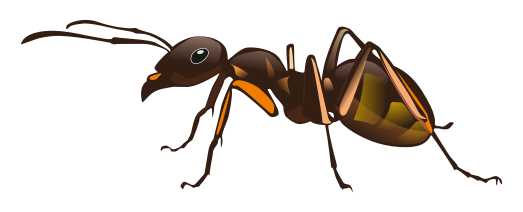
\includegraphics[width=\columnwidth]{Monsters/Animals/Ant, Giant}

\subsection{Ape, Cave}\index[monsters]{Cave Ape}
\statblock{\textbf{Size:} Medium

\textbf{Type:} Animal

\textbf{Habitat:} Mountains, Underground (Rare)

\textbf{Wandering Group:} 1d6 (Nil)

\textbf{Lair Group:} 2d4 (Nil)

\textbf{Move:} 40 ft.

\textbf{Armor Class:} 6

\textbf{Hit Dice:} 4 (18 HP)

\textbf{Attacks:} 2x Claw (1d4) or Rock (1d6)

\textbf{Special:} None

\textbf{Save:} F2

\textbf{Alignment:} None

\textbf{Intelligence:} 2

\textbf{Morale:} 7

\textbf{XP Value:} 75}

Cave apes are gorilla-like apes that have lived underground for generations, and have lost their coloring—leaving them white with pink eyes.

They are generally peaceful creatures, content to scavenge for fungus and mushrooms, and will flee from any strangers unless the strangers approach their lair.

Cave apes will noisily threaten any who come too close to their lair, and if the threats fail they will throw rocks at the intruders until they either leave or get close enough to fight in melee.

Cave apes are considerably less intelligent than the gorillas they descended from, although they are often tamed by \iref[monster:Neanderthal]{Neanderthals} and used as pets and guards.

\subsection{Ape, Rock Baboon}\index[monsters]{Rock Baboon}
\statblock{\textbf{Size:} Medium

\textbf{Type:} Animal

\textbf{Habitat:} Clear, Hills, Mountains (Common)

\textbf{Wandering Group:} 2d6 (U)

\textbf{Lair Group:} 5d6

\textbf{Move:} 40 ft.

\textbf{Armor Class:} 6

\textbf{Hit Dice:} 2 (9 HP)

\textbf{Attacks:} Club (1d6) \& Bite (1d3)

\textbf{Special:} None

\textbf{Save:} F2

\textbf{Alignment:} None

\textbf{Intelligence:} 2

\textbf{Morale:} 8

\textbf{XP Value:} 20}

Rock baboons are apes with short tails and long dog-like snouts. They are far more aggressive than most other apes, and are also more intelligent—although their use of tools is limited to picking up branches for use as rudimentary clubs.

Rock baboons will go out of their way to scare off anyone intruding into their territory, and won’t hesitate to resort to violence if intruders don’t leave quickly enough.

\subsection{Ape, Snow}\index[monsters]{Snow Ape}
\statblock{\textbf{Size:} Medium

\textbf{Type:} Animal

\textbf{Habitat:} Arctic (Rare)

\textbf{Wandering Group:} 1d6 (Nil)

\textbf{Lair Group:} 2d6 (K)

\textbf{Move:} 30 ft.

\textbf{Armor Class:} 6

\textbf{Hit Dice:} 3+1 (14 HP)

\textbf{Attacks:} Club (1d6) \& Hug (2d6)

\textbf{Special:} Blend, Squeeze

\textbf{Save:} F3

\textbf{Alignment:} Chaotic

\textbf{Intelligence:} 4

\textbf{Morale:} 7

\textbf{XP Value:} 50}

Snow apes are a (barely) sapient species of ape with long white fur.

Although sapient, snow apes have no spoken language, communicating only by sign language. They have no material culture, living out in the open and using no tools more advanced than a club.

Snow apes are very kind and caring to their own species, but violently xenophobic to all other species. They only consider creatures that can communicate with them to be intelligent, dismissing the speech of other humanoid races as just “animal noises”.

\textbf{Blend:} The snow ape's white fur makes them extremely difficult to spot in snowy terrain, allowing them to surprise opponents on a 1-4.

\textbf{Squeeze:} Snow apes are very strong, and if one succeeds with a hug attack, it will hold on to its victim automatically doing 2d6 damage per round.

\subsection{Athach}\index[monsters]{Athach}
\statblock{\textbf{Size:} Large

\textbf{Type:} Giant

\textbf{Habitat:} Hills, Mountains, Woods (Rare)

\textbf{Wandering Group:} 1d3 (Nil)

\textbf{Lair Group:} 1d6 (I)

\textbf{Move:} 60 ft.

\textbf{Armor Class:} 0

\textbf{Hit Dice:} 14* (63 HP)

\textbf{Attacks:} 3x Bash (2d12) \& Bite (2d10)

\textbf{Special:} Poison

\textbf{Save:} F14

\textbf{Alignment:} Chaotic

\textbf{Intelligence:} 8

\textbf{Morale:} 7

\textbf{XP Value:} 2,500}

An athach is a hideously deformed giant with three arms, their third arm protruding from their chests.

Athachs are rather stupid and very bad tempered, and will normally kill and eat anyone they meet who does not give them gems and jewelry. Athach families are violent affairs, and only the strongest and meanest children survive into adulthood—whereupon they almost always end up killing their aging and weakening parents.

Athachs normally attack by simply bashing their opponents with whatever comes to hand (rocks, tree stumps, and so on) and biting with their poisonous tusks.

\textbf{Poison:} Anyone bitten by an athach must make a saving throw vs. poison or be \iref[sec:Helpless]{Helpless} for 1d6 x 10 minutes.

\subsection{Basilisk}\index[monsters]{Basilisk}
\statblock{\textbf{Size:} Large

\textbf{Type:} Monster

\textbf{Habitat:} Woods, Underground (Rare), 

Elemental Plane of Earth (Very Rare)

\textbf{Wandering Group:} 1d6 (Nil)

\textbf{Lair Group:} 1d6 (F)

\textbf{Move:} 20 ft.

\textbf{Armor Class:} 4

\textbf{Hit Dice:} 6+1**

\textbf{Attacks:} Bite (1d10)

\textbf{Special:} Petrifying Gaze

\textbf{Save:} F6

\textbf{Alignment:} None

\textbf{Intelligence:} 2

\textbf{Morale:} 9

\textbf{XP Value:} 950}

A basilisk is a snake-like lizard with six legs and a crown-like crest on its head. Often called the “king of snakes”, it is feared for its deadly gaze.

Basilisks are not normally aggressive, eating only small animals which they must hunt by taking them by surprise in order to avoid accidentally turning them to stone.

\textbf{Petrifying Gaze:} Any creature meeting its gaze must make a saving throw vs. petrification or be turned to stone.

The gaze of a basilisk must be direct, seeing its reflection is not enough to have a chance of being turned to stone. However, a basilisk is not immune to its own gaze attack, and if presented with a mirror, there is a 1 in 6 chance per round that it will see its reflection and must make the saving throw to avoid petrifying itself. This is the only circumstance in which its gaze is effective through a mirror.

Any character surprised by a basilisk automatically meets its gaze and must make the saving throw, and in combat each character attacking the basilisk without actively avoiding the gaze must also make the saving throw each round.

Characters trying to fight the basilisk blindfolded or otherwise averting their gaze will not be affected but must attack with a -4 penalty to hit and the basilisk gets a +2 bonus against characters using such tactics.

A character using a mirror to attack in melee (the mirror takes one hand, so the character cannot use an off-hand weapon or a shield at the same time) takes only a -2 penalty to hit and the basilisk gets no bonus against them.

\subsubsection{Home Plane}
Basilisks originate from the \iref[sec:Elemental Plane of Earth]{Elemental Plane of Earth}. When on that plane they appear as a lizard-like creature made of rock.

\textbf{Petrifying Gaze:} When used against earth creatures, rather than being petrified they become slowed as the spell \ilink{spell:Slow}{Slow} for 1d6 rounds.

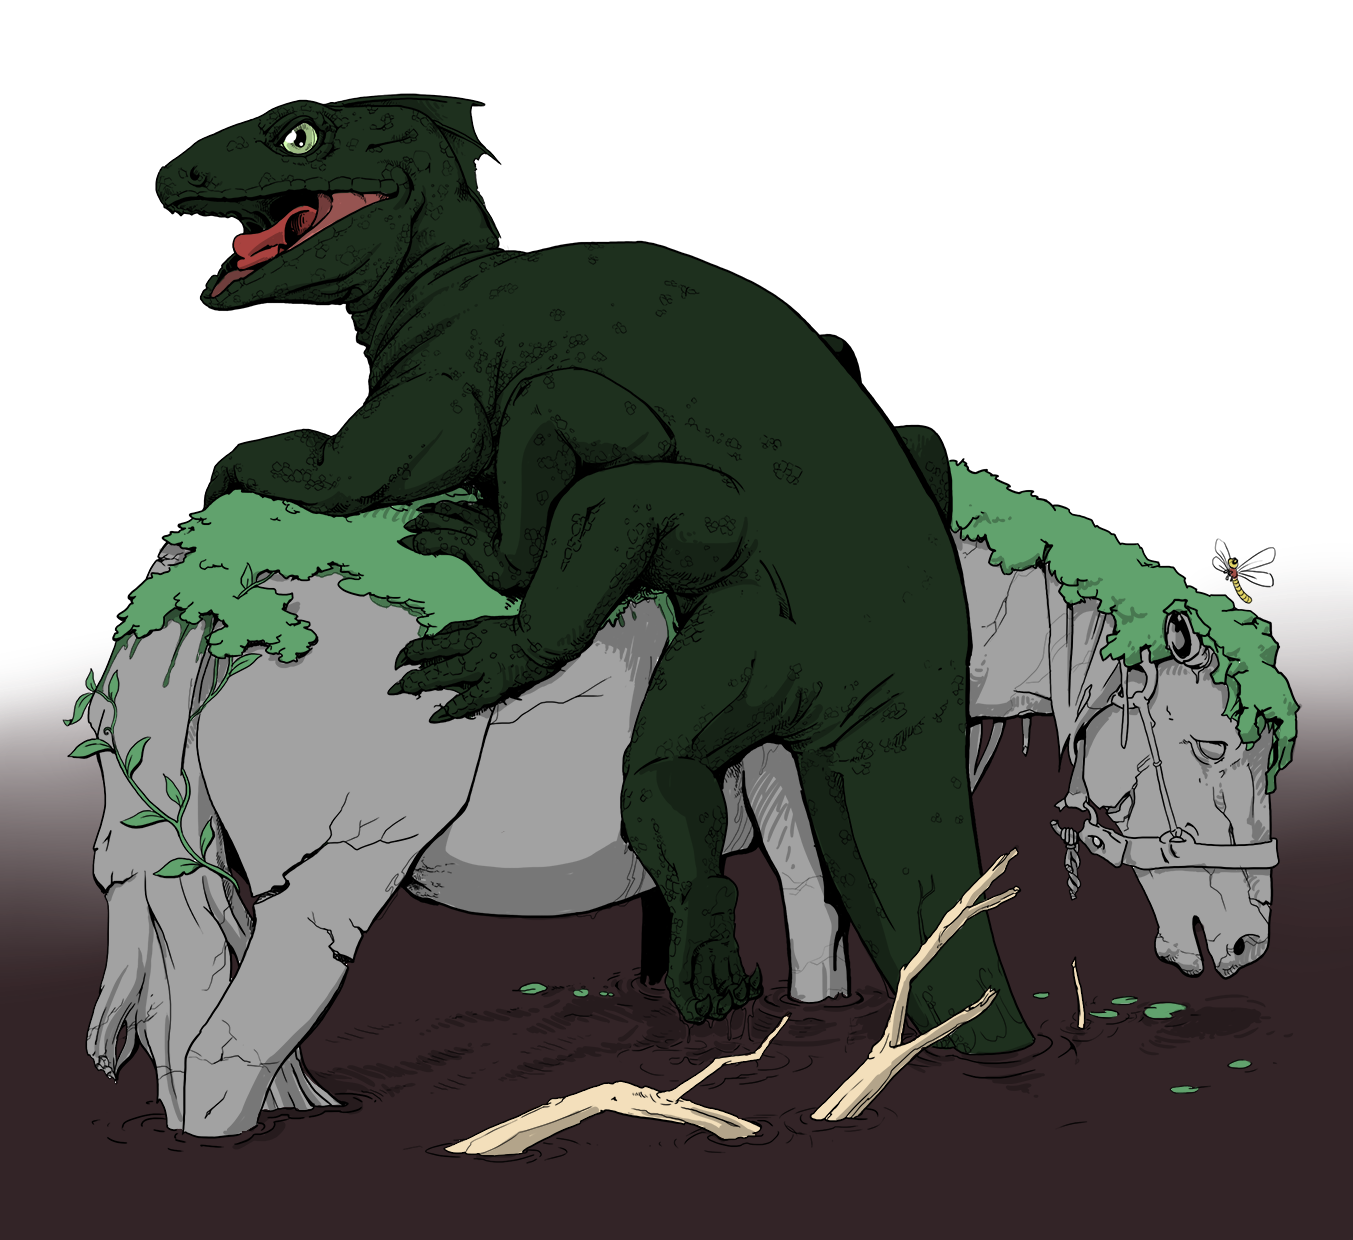
\includegraphics[width=\columnwidth]{Monsters/Basilisk}

\subsection{Bat}\index[monsters]{Bat}
\statblock{\textbf{Size:} Small

\textbf{Type:} Animal

\textbf{Habitat:} Underground (Common)

\textbf{Wandering Group:} 1d100 (Nil)

\textbf{Lair Group:} 1d100 (Nil)

\textbf{Move:} 3 ft., 40 ft. (Fly)

\textbf{Armor Class:} 6

\textbf{Hit Dice:} 1/4 (1 HP)

\textbf{Attacks:} Bite (1d2)

\textbf{Special:} Bewilder

\textbf{Save:} F0

\textbf{Alignment:} None

\textbf{Intelligence:} 2

\textbf{Morale:} 6

\textbf{XP Value:} 5}

Bats are nocturnal flying mammals, brown or black in color with leathery wings.

Bats are normally inoffensive and will not attack anything larger than a small insect.

\textbf{Bewilder:} When either panicking or controlled by another creature, a flock of bats can be very confusing as they fly around an opponent.

Any character with ten or more bats attacking them will be bewildered and suffer a -2 penalty on both to-hit rolls and saving throws. Additionally, a bewildered character may not cast spells.

\subsection{Vampire Bat}\index[monsters]{Vampire Bat}
Vampire bats are similar to other bats except that they have a paralyzing bite which allows them to drink blood.

\textbf{Create Undead:} Creatures slain by a giant vampire bat must make a saving throw vs. spells or return as an undead 24 hours later. The type of undead should be determined randomly by consulting \fullref{tab:Giant Vampire Bat}.

\begin {table}[H]
  \caption{Giant Vampire Bat}\label{tab:Giant Vampire Bat}
  \begin{tabularx}{\columnwidth}{>{\bfseries}YYYYY}
	\thead{1d6} & \thead{Type}\\
	1-3 & Zombie\\
	4-5 & Ghoul\\
	6 & Wight
  \end {tabularx}
\end {table}

\textbf{Drain Blood:} Anyone bitten by a giant vampire bat must make a saving throw vs. paralysis or be paralyzed for 1d10 rounds. Giant vampire bats can drain blood (for 1d4 damage per round) from paralyzed creatures, but will only start to do so when all their opponents are paralyzed in this manner.

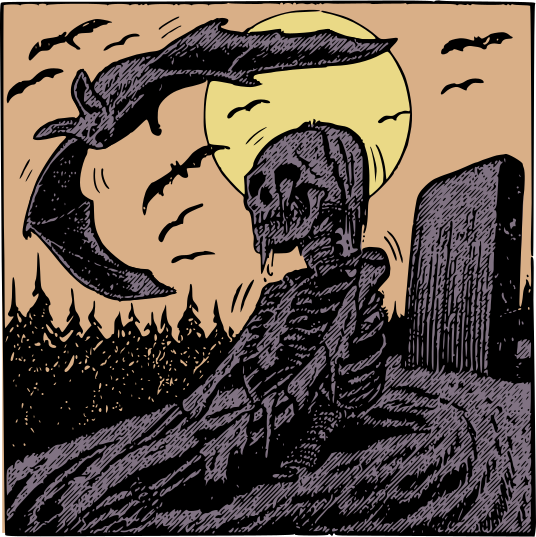
\includegraphics[width=\columnwidth]{Monsters/Animals/Bat, Giant Vampire}

\subsection{Bear}
\textbf{Hug:} If a bear hits with both claw attacks, it will hug the victim for an additional 2d8 damage.

\subsubsection{Black Bear}\index[monsters]{Black Bear}
\statblock{\textbf{Size:} Medium

\textbf{Type:} Animal

\textbf{Habitat:} Hills, Mountains, Woods (Common)

\textbf{Wandering Group:} 1d4 (U)

\textbf{Lair Group:} 1d4 (Nil)

\textbf{Move:} 40 ft.

\textbf{Armor Class:} 6

\textbf{Hit Dice:} 4 (18 HP)

\textbf{Attacks:} 2x Claw (1d3) \& Bite (1d6)

\textbf{Special:} Hug

\textbf{Save:} F2

\textbf{Alignment:} None

\textbf{Intelligence:} 2

\textbf{Morale:} 7

\textbf{XP Value:} 75}

Black bears are tall mammals covered with black fur.

Black bears survive on an omnivorous diet, particularly favoring fish. They are inquisitive creatures and will often raid camps looking for food.

\subsubsection{Cave Bear}\index[monsters]{Cave Bear}
\statblock{\textbf{Size:} Large

\textbf{Type:} Animal

\textbf{Habitat:} Hills, Mountains, Woods (Very Rare)

\textbf{Wandering Group:} 1d2 (V)

\textbf{Lair Group:} 1d2 (Nil)

\textbf{Move:} 40 ft.

\textbf{Armor Class:} 5

\textbf{Hit Dice:} 7 (28 HP)

\textbf{Attacks:} 2x Claw (2d4) \& Bite (2d6)

\textbf{Special:} Hug

\textbf{Save:} F4

\textbf{Alignment:} None

\textbf{Intelligence:} 2

\textbf{Morale:} 9

\textbf{XP Value:} 450}

Cave bears are larger versions of brown bears.

Cave bears are particularly aggressive bears.

Unlike most bears they are exclusively carnivorous, and are active hunters.

\subsubsection{Grizzly Bear}\index[monsters]{Grizzly Bear}
\monsterimage{Monsters/Animals/Bear, Brown}{\statblock{\textbf{Size:} Large

\textbf{Type:} Animal

\textbf{Habitat:} Hills, 

Mountains, Woods (Common)

\textbf{Wandering Group:} 1 (U)

\textbf{Lair Group:} 1d4 (Nil)

\textbf{Move:} 40 ft.

\textbf{Armor Class:} 8

\textbf{Hit Dice:} 5 (23 HP)

\textbf{Attacks:} 2x Claw (1d8) \& Bite (1d10)

\textbf{Special:} Hug

\textbf{Save:} F4

\textbf{Alignment:} None

\textbf{Intelligence:} 2

\textbf{Morale:} 10

\textbf{XP Value:} 175}}

Grizzly bears are tall mammals covered with silver-tipped brown or reddish brown fur.

Grizzly bears have a widely varied omnivorous diet, preferring fruit and fish; although they will also hunt small animals.

They won’t attack humanoids for food, although they are notoriously short tempered and territorial, and will chase and fight those who come too near, particularly in the spring after the females emerge from hibernation and give birth. The ferocity of mother grizzly bears protecting their cubs is legendary.

\subsubsection{Polar Bear}\index[monsters]{Polar Bear}
\statblock{\textbf{Size:} Large

\textbf{Type:} Animal

\textbf{Habitat:} Arctic (Rare)

\textbf{Wandering Group:} 1 (U)

\textbf{Lair Group:} 1d2 (Nil)

\textbf{Move:} 40 ft.

\textbf{Armor Class:} 6

\textbf{Hit Dice:} 6 (27 HP)

\textbf{Attacks:} 2x Claw (1d6) \& Bite (1d10)

\textbf{Special:} Hug

\textbf{Save:} F3

\textbf{Alignment:} None

\textbf{Intelligence:} 2

\textbf{Morale:} 8

\textbf{XP Value:} 275}

Polar bears are tall mammals covered with white fur.

Polar bears are carnivorous. Their normal diet consists of fish and seals, and they encounter humanoids rarely enough that they have no fear of them and see them as another source of food.

\subsection{Bee, Giant}\index[monsters]{Giant Bee}
\monsterimage{Monsters/Animals/Bee, Giant}{\statblock{\textbf{Size:} Small

\textbf{Type:} Animal

\textbf{Habitat:} Hills, Mountains, Woods (Rare)

\textbf{Wandering Group:} 1d6 (Nil)

\textbf{Lair Group:} 5d6 (See Below)

\textbf{Move:} 50 ft.

\textbf{Armor Class:} 7

\textbf{Hit Dice:} ½* (3 HP)

\textbf{Attacks:} Sting (1d3)

\textbf{Special:} Poison

\textbf{Save:} F1

\textbf{Alignment:} None

\textbf{Intelligence:} 0

\textbf{Morale:} 9 (See Below)

\textbf{XP Value:} 6}}

Giant bees are larger versions of regular bees. They are normally peaceful when out collecting pollen and fruit, and will ignore creatures that do not molest them, fighting only in self defense.

However, any creature that comes within 30 feet of their hive will be attacked by every bee in the hive and the colony will fight to the death.

The hive will contain a non-combatant queen bee, and her 1d4+2 drones, each of which has 1 hit dice (5 HP, 13 XP).

A giant bee hive will contain about two pints of honey, which can be distilled down into a single \iref[mitem:Potion of Healing]{Potion of Healing}.

\textbf{Poison:} When a giant bee stings an opponent, the opponent must make a saving throw vs. poison or die. However, the attacking bee is always killed by the attack, as the stinger comes loose and sticks in the wound.

A character with a giant bee sting in them continues to lose one hit point per round until they spend an action removing the stinger, although they need not make further saving throws vs. poison after the initial sting.

\subsection{Beetle, Giant Bombard}\index[monsters]{Giant Bombard Beetle}
\statblock{\textbf{Size:} Small

\textbf{Type:} Animal

\textbf{Habitat:} Clear, Underground, Woods (Common)

\textbf{Wandering Group:} 1d8 (Nil)

\textbf{Lair Group:} 2d6 (Nil)

\textbf{Move:} 40 ft.

\textbf{Armor Class:} 4

\textbf{Hit Dice:} 2* (9 HP)

\textbf{Attacks:} Bite (1d6)

\textbf{Special:} Acid Spray

\textbf{Save:} F1

\textbf{Alignment:} None

\textbf{Intelligence:} 0

\textbf{Morale:} 8

\textbf{XP Value:} 25}

Giant bombard beetles have a dark elytra and an orangish head.

\textbf{Acid Spray:} When surprised or attacked, a giant bombard beetle will respond by squirting a hot acid at a foe within 5 feet (it can only do this once per combat, and will do so at the earliest opportunity). This acid is not enough to cause significant damage, but it is highly irritant and causes the target to take a -2 penalty to attack rolls and ability checks for the next 24 hours or until the victim is cured by a Cure Light Wounds spell.

\subsection{Beetle, Giant Fire}\index[monsters]{Giant Fire Beetle}
\statblock{\textbf{Size:} Small

\textbf{Type:} Animal

\textbf{Habitat:} Clear, Underground, Woods (Common)

\textbf{Wandering Group:} 1d8 (Nil)

\textbf{Lair Group:} 2d6 (Nil)

\textbf{Move:} 40 ft.

\textbf{Armor Class:} 4

\textbf{Hit Dice:} 1+2 (7 HP)

\textbf{Attacks:} Bite (2d4)

\textbf{Special:} 

\textbf{Save:} F1

\textbf{Alignment:} None

\textbf{Intelligence:} 0

\textbf{Morale:} 7

\textbf{XP Value:} 15}

Giant fire beetles have glowing red spots above their eyes that give off normal (non-magical) light within a 10-foot radius, about the strength of a single candle.

If removed, the glands will continue to glow for 1d6 days before fading.

\subsection{Beetle, Giant Tiger}\index[monsters]{Beetle, Giant Tiger}
\statblock{\textbf{Size:} Small

\textbf{Type:} Animal

\textbf{Habitat:} Clear, Underground, Woods (Common)

\textbf{Wandering Group:} 1d6 (Nil)

\textbf{Lair Group:} 2d4 (Nil)

\textbf{Move:} 50 ft.

\textbf{Armor Class:} 3

\textbf{Hit Dice:} 3+1 (15 HP)

\textbf{Attacks:} Bite (2d6)

\textbf{Special:} None

\textbf{Save:} F2

\textbf{Alignment:} None

\textbf{Intelligence:} 0

\textbf{Morale:} 9

\textbf{XP Value:} 50}

Giant tiger beetles have large (2 feet long) mandibles that they use to bite prey.

They will not normally attack creatures larger than themselves unless they are either cornered or starving.

\subsection{Bhut}\index[monsters]{Bhut}
\statblock{\textbf{Size:} Medium

\textbf{Type:} Undead

\textbf{Habitat:} Settled (Very Rare)

\textbf{Wandering Group:} 2d4 (Nil)

\textbf{Lair Group:} 2d4 (A)

\textbf{Move:} 120 ft., 40 ft. (Fly)

\textbf{Armor Class:} 4

\textbf{Hit Dice:} 7+2** (33hp)

\textbf{Attacks:} 2x Claw (1d4) \& Bite (1d6)

\textbf{Special:} Frost Bite, Immunity (Mind Effects, Poison), Shapechange

\textbf{Save:} F10

\textbf{Alignment:} Chaotic

\textbf{Intelligence:} 12

\textbf{Morale:} 10

\textbf{XP Value:} 1,500}

A bhut is an undead spirit that has died a violent death or have been denied funeral rites. Bhuts have wild hair, claws, long sharp teeth, and backwards feet. When walking, the bhuts feet never touch the ground, they float about a centimeter from it. Bhuts eat human and demi-human flesh. They prefer to reside in abandoned locations near or in human or demi-human settlements, as to be closer to their prey.

\textbf{Frost Bite:} The teeth of a bhut are freezing cold, which causes anyone that is bitten by them to roll a save vs. paralysis or be numbed for 1d4 rounds. While numbed the victim always looses initiative and suffers a -2 to all attack rolls.

\textbf{Shapechange:} A bhut can assume the form of any animal at will. They look exactly like the animal of their choice except the feet on the bhuts new form are still backwards. The bhuts attributes do not change when assuming this new form.

\subsection{Bird of Prey}\index[monsters]{Bird of Prey}\label{monster:Bird of Prey}
\monsterimage{Monsters/Animals/Bird of Prey}{\statblock{\textbf{Size:} Small

\textbf{Type:} Animal

\textbf{Habitat:} Any (Common)

\textbf{Wandering Group:} 1 (Nil)

\textbf{Lair Group:} 1d6 (Nil)

\textbf{Move:} 5 ft., 60 ft. (Fly)

\textbf{Armour Class:} 8

\textbf{Hit Dice:} 1d4 HP

\textbf{Attacks:} 2x Claw (1d2) or Bite (1d4)

\textbf{Special:} None

\textbf{Save:} F0

\textbf{Alignment:} None

\textbf{Intelligence:} 2

\textbf{Morale:} 7

\textbf{XP Value:} 5}}

Birds of prey, or raptors, are hunting birds that feed on other animals. They have keen vision that allows them to spot prey from a great distance. Birds of prey tend to build their nests in lofty areas, such as near a mountain top or up in a very large tree top. Buzzards, falcons, harriers, hawks, eagles, kites, osprey, owls, and vultures are all considered birds of prey.

When either themselves or their nest is threatened, birds of prey will attack with their powerful talons or beaks. If injured, they will retreat.

\subsection{Black Pudding}\index[monsters]{Black Pudding}
\statblock{\textbf{Size:} Large

\textbf{Type:} Ooze

\textbf{Habitat:} Underground (Common)

\textbf{Wandering Group:} 1 (See Below)

\textbf{Lair Group:} 1 (See Below)

\textbf{Move:} 20 ft.

\textbf{Armor Class:} 6*

\textbf{Hit Dice:} 10* (45 HP)

\textbf{Attacks:} Touch (3d8)

\textbf{Special:} Amorphous, Dissolve, Spider Climb, Split

\textbf{Save:} F5

\textbf{Alignment:} None

\textbf{Intelligence:} 0

\textbf{Morale:} 12

\textbf{XP Value:} 1,750}

A black pudding is a dark colored ooze that has no intelligence or instinct other than to absorb and digest anything they can get to. As such they will always attack and fight to the death, and will do such unintelligent things as moving straight through fire to get to an opponent rather than avoiding it.

Black puddings are very resilient, and fire is the only thing that can kill them.

Black puddings do not carry treasure, but the area around them may contain indigestible gemstones (the only remains of those that have been eaten by the pudding).

\textbf{Amorphous:} Despite their size, black puddings can squeeze their bulk through holes as small as an inch in diameter (although doing so will be very slow, taking 10 minutes.

\textbf{Dissolve:} A black pudding can dissolve a wood or metal object the size of a normal door in 10 minutes, but cannot eat through stone.

\textbf{Spider Climb:} Black puddings can move along walls or ceilings as easily as floors.

\textbf{Split:} Psychical attacks will split the pudding into 2 HD chunks that do only 1d8 damage. These smaller puddings can not be further damaged apart from by fire.

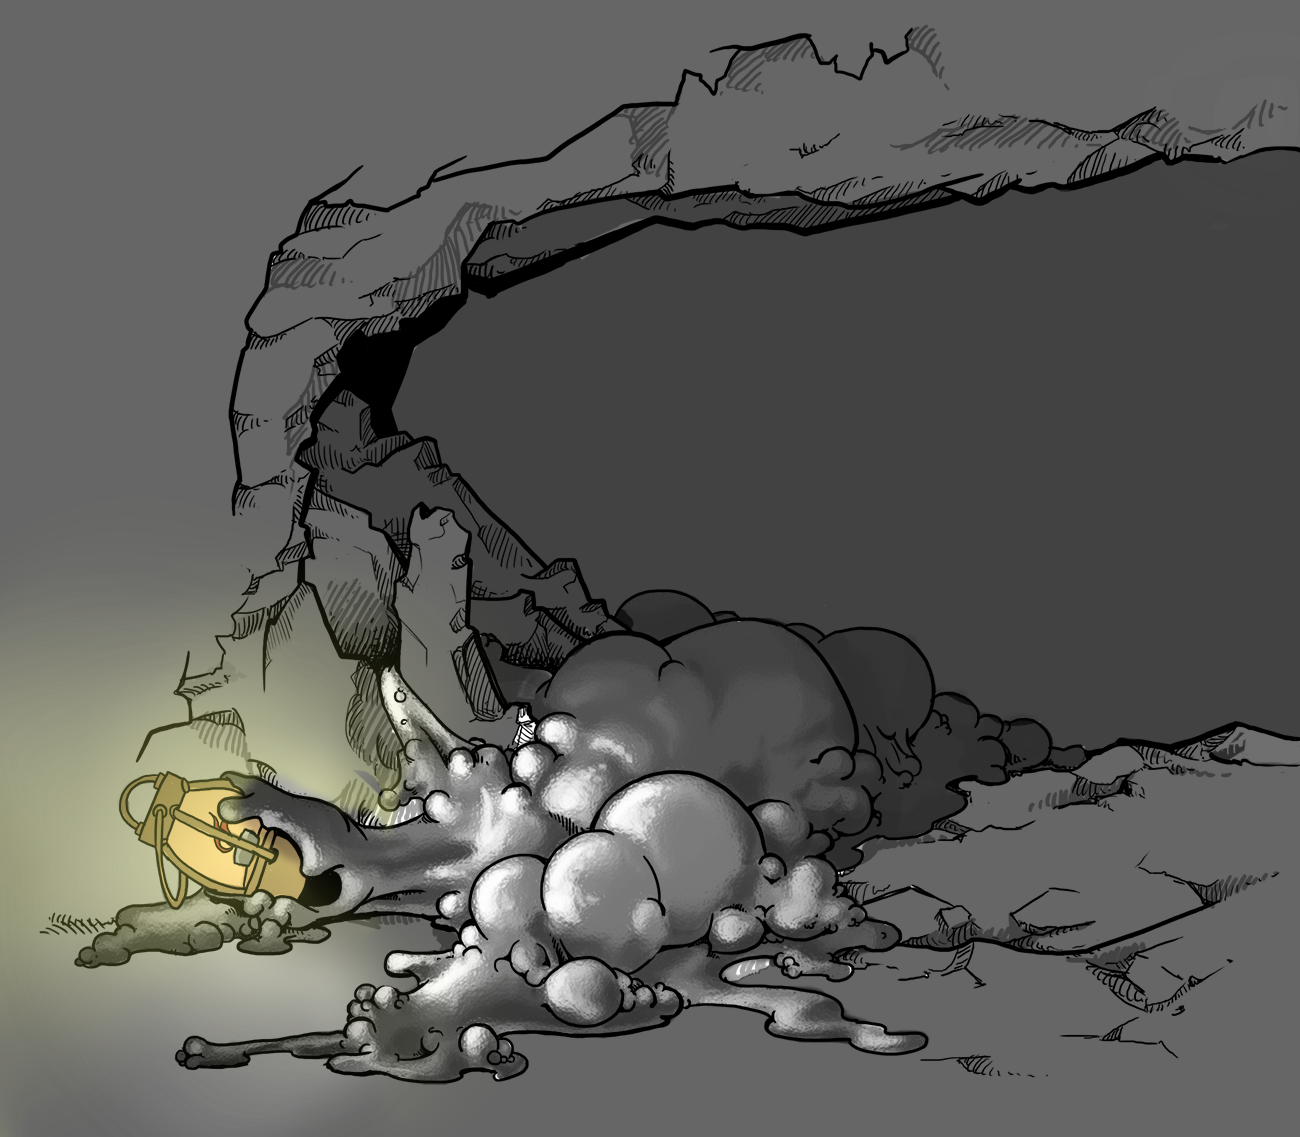
\includegraphics[width=\columnwidth]{Monsters/Black Pudding}

\subsection{Blackball}\index[monsters]{Blackball}
\statblock{\textbf{Size:} Medium

\textbf{Type:} Extraplanar

\textbf{Habitat:} Any (Very Rare)

\textbf{Wandering Group:} 1 (Nil)

\textbf{Lair Group:} 1 (Nil)

\textbf{Move:} 10 ft.

\textbf{Armor Class:} 9*

\textbf{Hit Dice:} See Below

\textbf{Attacks:} Touch (See Below)

\textbf{Special:} Efface, Immunity to Everything

\textbf{Save:} F34

\textbf{Alignment:} See Below

\textbf{Intelligence:} See Below

\textbf{Morale:} 12

\textbf{XP Value:} 7,500}

Blackballs may be the most enigmatic and powerful of creatures, and even \iref[chap:Immortals]{Immortals} are afraid of them. Or they may not be creatures at all. No-one knows for certain.

A blackball is a featureless flying sphere that is pure black in color (no light is reflected from it).

Blackballs can spend centuries or even millennia simply sitting motionless in one place. Then for no explicable reason one may suddenly start moving—eating its way through rock and metal and even Force Field spells without slowing down. It will travel for miles, and even cross planes through gates or natural boundaries, until it gets to a specific creature or object; and then it destroys that target and lays dormant again.

Although their behavior while moving appears to be intelligent, no-one has ever been able to communicate meaningfully with a blackball, and no magic is able to read (or even detect) its mind.

\textbf{Efface:} Anything a blackball touches simply disappears utterly (no saving throw) leaving absolutely no trace, although this ability appears to be at least somewhat controlled, since a blackball can travel through air or water without destroying them.

\textbf{Immunity to Everything:} Blackballs are utterly immune to everything and cannot be controlled or harmed in any way except that they are subject to the Teleport spell.

\subsection{Blink Dog}\index[monsters]{Blink Dog}
\statblock{\textbf{Size:} Medium

\textbf{Type:} Monster

\textbf{Habitat:} Clear, Desert, Woods (Common)

\textbf{Wandering Group:} 1d6 (Nil)

\textbf{Lair Group:} 1d6+3 (C)

\textbf{Move:} 40 ft.

\textbf{Armor Class:} 5

\textbf{Hit Dice:} 4* (18 HP)

\textbf{Attacks:} Bite (1d6)

\textbf{Special:} Teleport

\textbf{Save:} F4

\textbf{Alignment:} Lawful

\textbf{Intelligence:} 9

\textbf{Morale:} 6

\textbf{XP Value:} 125}

Blink dogs are intelligent wild dogs with the ability to teleport from place to place. They are smaller than wolves, and more jackal-like in appearance.

Blink dogs have their own language, but unfortunately their mouths are shaped wrongly for speaking humanoid tongues, although they often understand them. Blink dogs are friendly towards humans and demi-humans, and will often live near rural villages for mutual benefit.

\textbf{Teleport:} Blink dogs can teleport at will, although their teleports (or “blinks”) are only short range (40 feet at the most). They will instinctively avoid teleporting into objects. In combat, their preferred tactic is teleport up to a victim, bite them, and then immediately teleport 1d4x10 feet away.

\subsection{Boar}\index[monsters]{Boar}
\statblock{\textbf{Size:} Medium

\textbf{Type:} Animal

\textbf{Habitat:} Woods (Common)

\textbf{Wandering Group:} 1d6 (Nil)

\textbf{Lair Group:} 1d6 (Nil)

\textbf{Move:} 30 ft.

\textbf{Armor Class:} 7

\textbf{Hit Dice:} 3* (13 HP)

\textbf{Attacks:} Tusk (2d4)

\textbf{Special:} Charge

\textbf{Save:} F2

\textbf{Alignment:} None

\textbf{Intelligence:} 2

\textbf{Morale:} 9

\textbf{XP Value:} 50}

Boars are the larger wild relatives of pigs. They are notoriously bad tempered and territorial, and will often attack even large opponents at the slightest provocation.

\textbf{Charge:} A boar can do a Charge action in combat. If it charges for 20 feet or more it does double damage on its attack, but is vulnerable to people doing \iref[sec:Set Spear]{Set Spear} actions.

\subsection{Brownie}\index[monsters]{Brownie}
\statblock{\textbf{Size:} Small

\textbf{Type:} Fey

\textbf{Habitat:} Settled, Woods (Rare)

\textbf{Wandering Group:} 0 (Nil)

\textbf{Lair Group:} 1 (Nil)

\textbf{Move:} 40 ft.

\textbf{Armor Class:} 7

\textbf{Hit Dice:} 2* (9 HP)

\textbf{Attacks:} Weapon (By weapon)

\textbf{Special:} Invisibility to Mortals

\textbf{Save:} H2

\textbf{Alignment:} Lawful

\textbf{Intelligence:} 

\textbf{Morale:} 8

\textbf{XP Value:} 25}

Brownies are homely humanoids that tend to live in the homes of humans that are in or near woodlands. They are around 2 1/2 feet and will usually be found wearing a brown hood or cloak. All known brownies are male. Female brownies may exist, but are either very rare or are indistinguishable from males in appearance and behavior.

Brownies will attach themselves to a home and will do chores late at night while the household is sleeping. Brownies do not require payment for this work, and any such offer would be taken as an insult. Small treats and praise will keep a brownie happy. If the brownie becomes unhappy, by getting low quality treats or having their work criticized, they will cause mischief around the home.

The only way to get rid of a brownie is to leave tiny clothes laid out for him. The brownie will leave immediately after seeing them.

\subsubsection{As a Class}\index[classes]{Brownie}
Brownies can be used as a class using the following statistics:

\statblock{\textbf{Ability Requirements:} Strength 5, Dexterity 8

\textbf{Prime Requisite:} Dexterity

\textbf{Ability Modifiers:} None

\textbf{Weapons:} Daggers, Miniature Weapons

\textbf{Armor:} Any

\textbf{Natural AC:} 9

\textbf{Special Abilities:} Invisibility to Mortals

\textbf{Magic Item Use:} Dwarf, Fighter, Halfling; Elf and Wizard (Chance of Misuse, see \fullref{tab:Brownie Magic Item Use})}

\begin {table}[H]
  \caption{Brownie Progression}
  \begin{tabularx}{\columnwidth}{>{\bfseries}YYY}
	\thead{Level} & \thead{Experience} & \thead{Hit Dice}\\
	-1 & -2,000 & 1d8\\
	0 & 0 & 2d8\\
	1 & 2,000 & 3d8\\
	2 & 6,000 & 4d8\\
	3 & 14,000 & 5d8\\
	4 & 30,500 & -\\
	5 & 62,000 & 6d8\\
	6 & 125,000 & 7d8\\
	7 & 250,000 & 8d8\\
	8 & 500,000 & 9d8\\
	9 & 800,000 & 10d8\\
	10+ & +300,000 & +2 HP
  \end {tabularx}
\end {table}

\begin {table}[H]
  \caption{Brownie Magic Item Use}\label{tab:Brownie Magic Item Use}
  \begin{tabularx}{\columnwidth}{>{\bfseries}YYYYY}
	\thead{} & \multicolumn{4}{c}{\thead{d\% Result}}\\
	\thead{Level} & \thead{Success} & \thead{Failure} & \thead{Backfire} & \thead{Unexpected}\\
	1 & 01-05 & 06-89 & 90-99 & 00\\
	2 & 01-05 & 06-89 & 90-98 & 99-00\\
	3 & 01-10 & 11-89 & 90-97 & 98-00\\
	4 & 01-15 & 16-89 & 90-96 & 97-00\\
	5 & 01-15 & 16-89 & 90-95 & 96-00\\
	6 & 01-20 & 21-89 & 90-94 & 95-00\\
	7 & 01-20 & 21-89 & 90-93 & 94-00\\
	8 & 01-25 & 26-89 & 90-92 & 93-00\\
	9 & 01-25 & 26-89 & 90-91 & 92-00\\
	10+ & 01-30 & 31-89 & 90 & 91-00
  \end {tabularx}
\end {table}

\subsection{Bugbear}\index[monsters]{Bugbear}
\statblock{\textbf{Size:} Medium

\textbf{Type:} Humanoid

\textbf{Habitat:} Hills, Mountains, Underground, Woods (Common)

\textbf{Wandering Group:} 2d8 (P+Q)

\textbf{Lair Group:} 5d4 (B)

\textbf{Move:} 30 ft.

\textbf{Armor Class:} 5

\textbf{Hit Dice:} 3+1 (14 HP)

\textbf{Attacks:} Weapon (By weapon + 1)

\textbf{Special:} Stealth

\textbf{Save:} F3

\textbf{Alignment:} Chaotic

\textbf{Intelligence:} 7

\textbf{Morale:} 9

\textbf{XP Value:} 50}

Bugbears are large and strong creatures related to goblins.

They have brown furred bodies, with round orange heads that look remarkably like carved pumpkins.

Bugbears are not the smartest of humanoids, and their technology is limited to simple spears and knives. They live as hunters, and will often raid farms for livestock. Sometimes bugbears will live with goblins as hired muscle, although they rarely lead goblin tribes as the goblins can out-think them.

\textbf{Stealth:} Despite their appearance, bugbears are stealthy and surprise opponents on a 1-3.

\subsubsection{Spellcasting}
The most intelligent bugbears can become shamans (up to level 6) or sorcerers (up to level 4).

\subsubsection{As a Class}\index[classes]{Bugbear}
Bugbears can be used as a class using the following statistics:

\statblock{\textbf{Ability Requirements:} Strength 13

\textbf{Prime Requisite:} Strength, Dexterity, Intelligence, or Wisdom

\textbf{Ability Modifiers:} Strength +1, Constitution +1, Wisdom -2

\textbf{Weapons:} Any

\textbf{Armor:} Any

\textbf{Natural AC:} 8

\textbf{Special Abilities:} Stealth

\textbf{Magic Item Use:} Fighter}

\begin {table}[H]
  \caption{Bugbear Progression}
  \begin{tabularx}{\columnwidth}{>{\bfseries}YYY}
	\thead{Level} & \thead{Experience} & \thead{Hit Dice}\\
	-2 & -2,400 & 1d8+1\\
	-1 & -1,200 & 2d8+1\\
	0 & 0 & 3d8+1\\
	1 & 2,400 & 4d8+2\\
	2 & 7,200 & 5d8+2\\
	3 & 16,600 & -\\
	4 & 35,600 & 6d8+2\\
	5 & 73,600 & 7d8+3\\
	6 & 147,600 & 8d8+3\\
	7 & 297,600 & -\\
	8 & 597,600 & 9d8+3\\
	9+ & +300,000 & +2 HP
  \end {tabularx}
\end {table}

\subsection{Caecilian, Giant}\index[monsters]{Giant Caecilian}
\statblock{\textbf{Size:} Large

\textbf{Type:} Animal

\textbf{Habitat:} Any except Arctic (Rare)

\textbf{Wandering Group:} 1d3 (Nil)

\textbf{Lair Group:} 1d3 (B)

\textbf{Move:} 20 ft.

\textbf{Armor Class:} 6

\textbf{Hit Dice:} 6* (27 HP)

\textbf{Attacks:} Bite (1d8)

\textbf{Special:} Swallow Whole

\textbf{Save:} F3

\textbf{Alignment:} None

\textbf{Intelligence:} 0

\textbf{Morale:} 9

\textbf{XP Value:} 500}

Much like their smaller cousins, caecilians are carnivorous amphibians that burrow into damp soil and earth and hunt by ambushing smaller creatures that walk over them.

\textbf{Swallow Whole:} Giant caecilians can swallow whole any creature human-sized or smaller that they bite if they roll an unmodified 19 or 20 and the attack hits. Swallowed creatures take 1d8 damage per round until they or the caecilian are killed.

\subsection{Camel}\index[monsters]{Camel}\label{monster:Camel}
\statblock{\textbf{Size:} Large

\textbf{Type:} Animal

\textbf{Habitat:} Barren Land, Desert (Common)

\textbf{Wandering Group:} Nil (Nil)

\textbf{Lair Group:} 2d4 (Nil)

\textbf{Move:} 50 ft.

\textbf{Armor Class:} 7

\textbf{Hit Dice:} 2 (9 HP)

\textbf{Attacks:} Bite (1) \& Kick (1d4)

\textbf{Special:} None

\textbf{Save:} F1

\textbf{Alignment:} None

\textbf{Intelligence:} 2

\textbf{Morale:} 7

\textbf{XP Value:} 20}

Camels are large domesticated beasts of burden that are well adapted for desert environments.

Camels have one or two distinctive “humps” on their back which are full of fat deposits. These humps can allow the camel for travel for long periods without needing to eat or drink.

Camels are commonly used by desert tribes for meat, milk and transport.

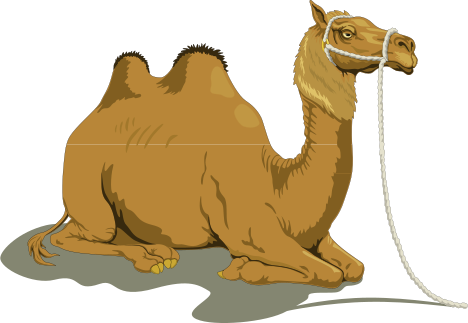
\includegraphics[width=\columnwidth]{Monsters/Animals/Camel}

\subsection{Cat, Jaguar}\index[monsters]{Jaguar}\label{monster:Jaguar}
\statblock{\textbf{Size:} Large

\textbf{Type:} Animal

\textbf{Habitat:} Jungle, Woods (Common)

\textbf{Wandering Group:} 1 (U)

\textbf{Lair Group:} 1d3 (Nil)

\textbf{Move:} 60 ft.

\textbf{Armor Class:} 6

\textbf{Hit Dice:} 4+2 (20 HP)

\textbf{Attacks:} 2x Claw (1d3)

\& Bite (1d8)

\textbf{Special:} Camouflage, Rake

\textbf{Save:} F2

\textbf{Alignment:} None

\textbf{Intelligence:} 2

\textbf{Morale:} 11

\textbf{XP Value:} 125}

Jaguars are cats that are extremely aggressive. They will attack any creature that they feel threatened by.

\textbf{Camouflage:} The werejaguar's markings provide remarkably effective camouflage in wooded surroundings, causing the werejaguar to surprise their opponents on a 1-3 on 1d6.

\textbf{Rake:} If the werejaguar successfully hits an opponent with both front claws, they automatically hit with their both of their back claws causing 1d4+1 damage per claw.

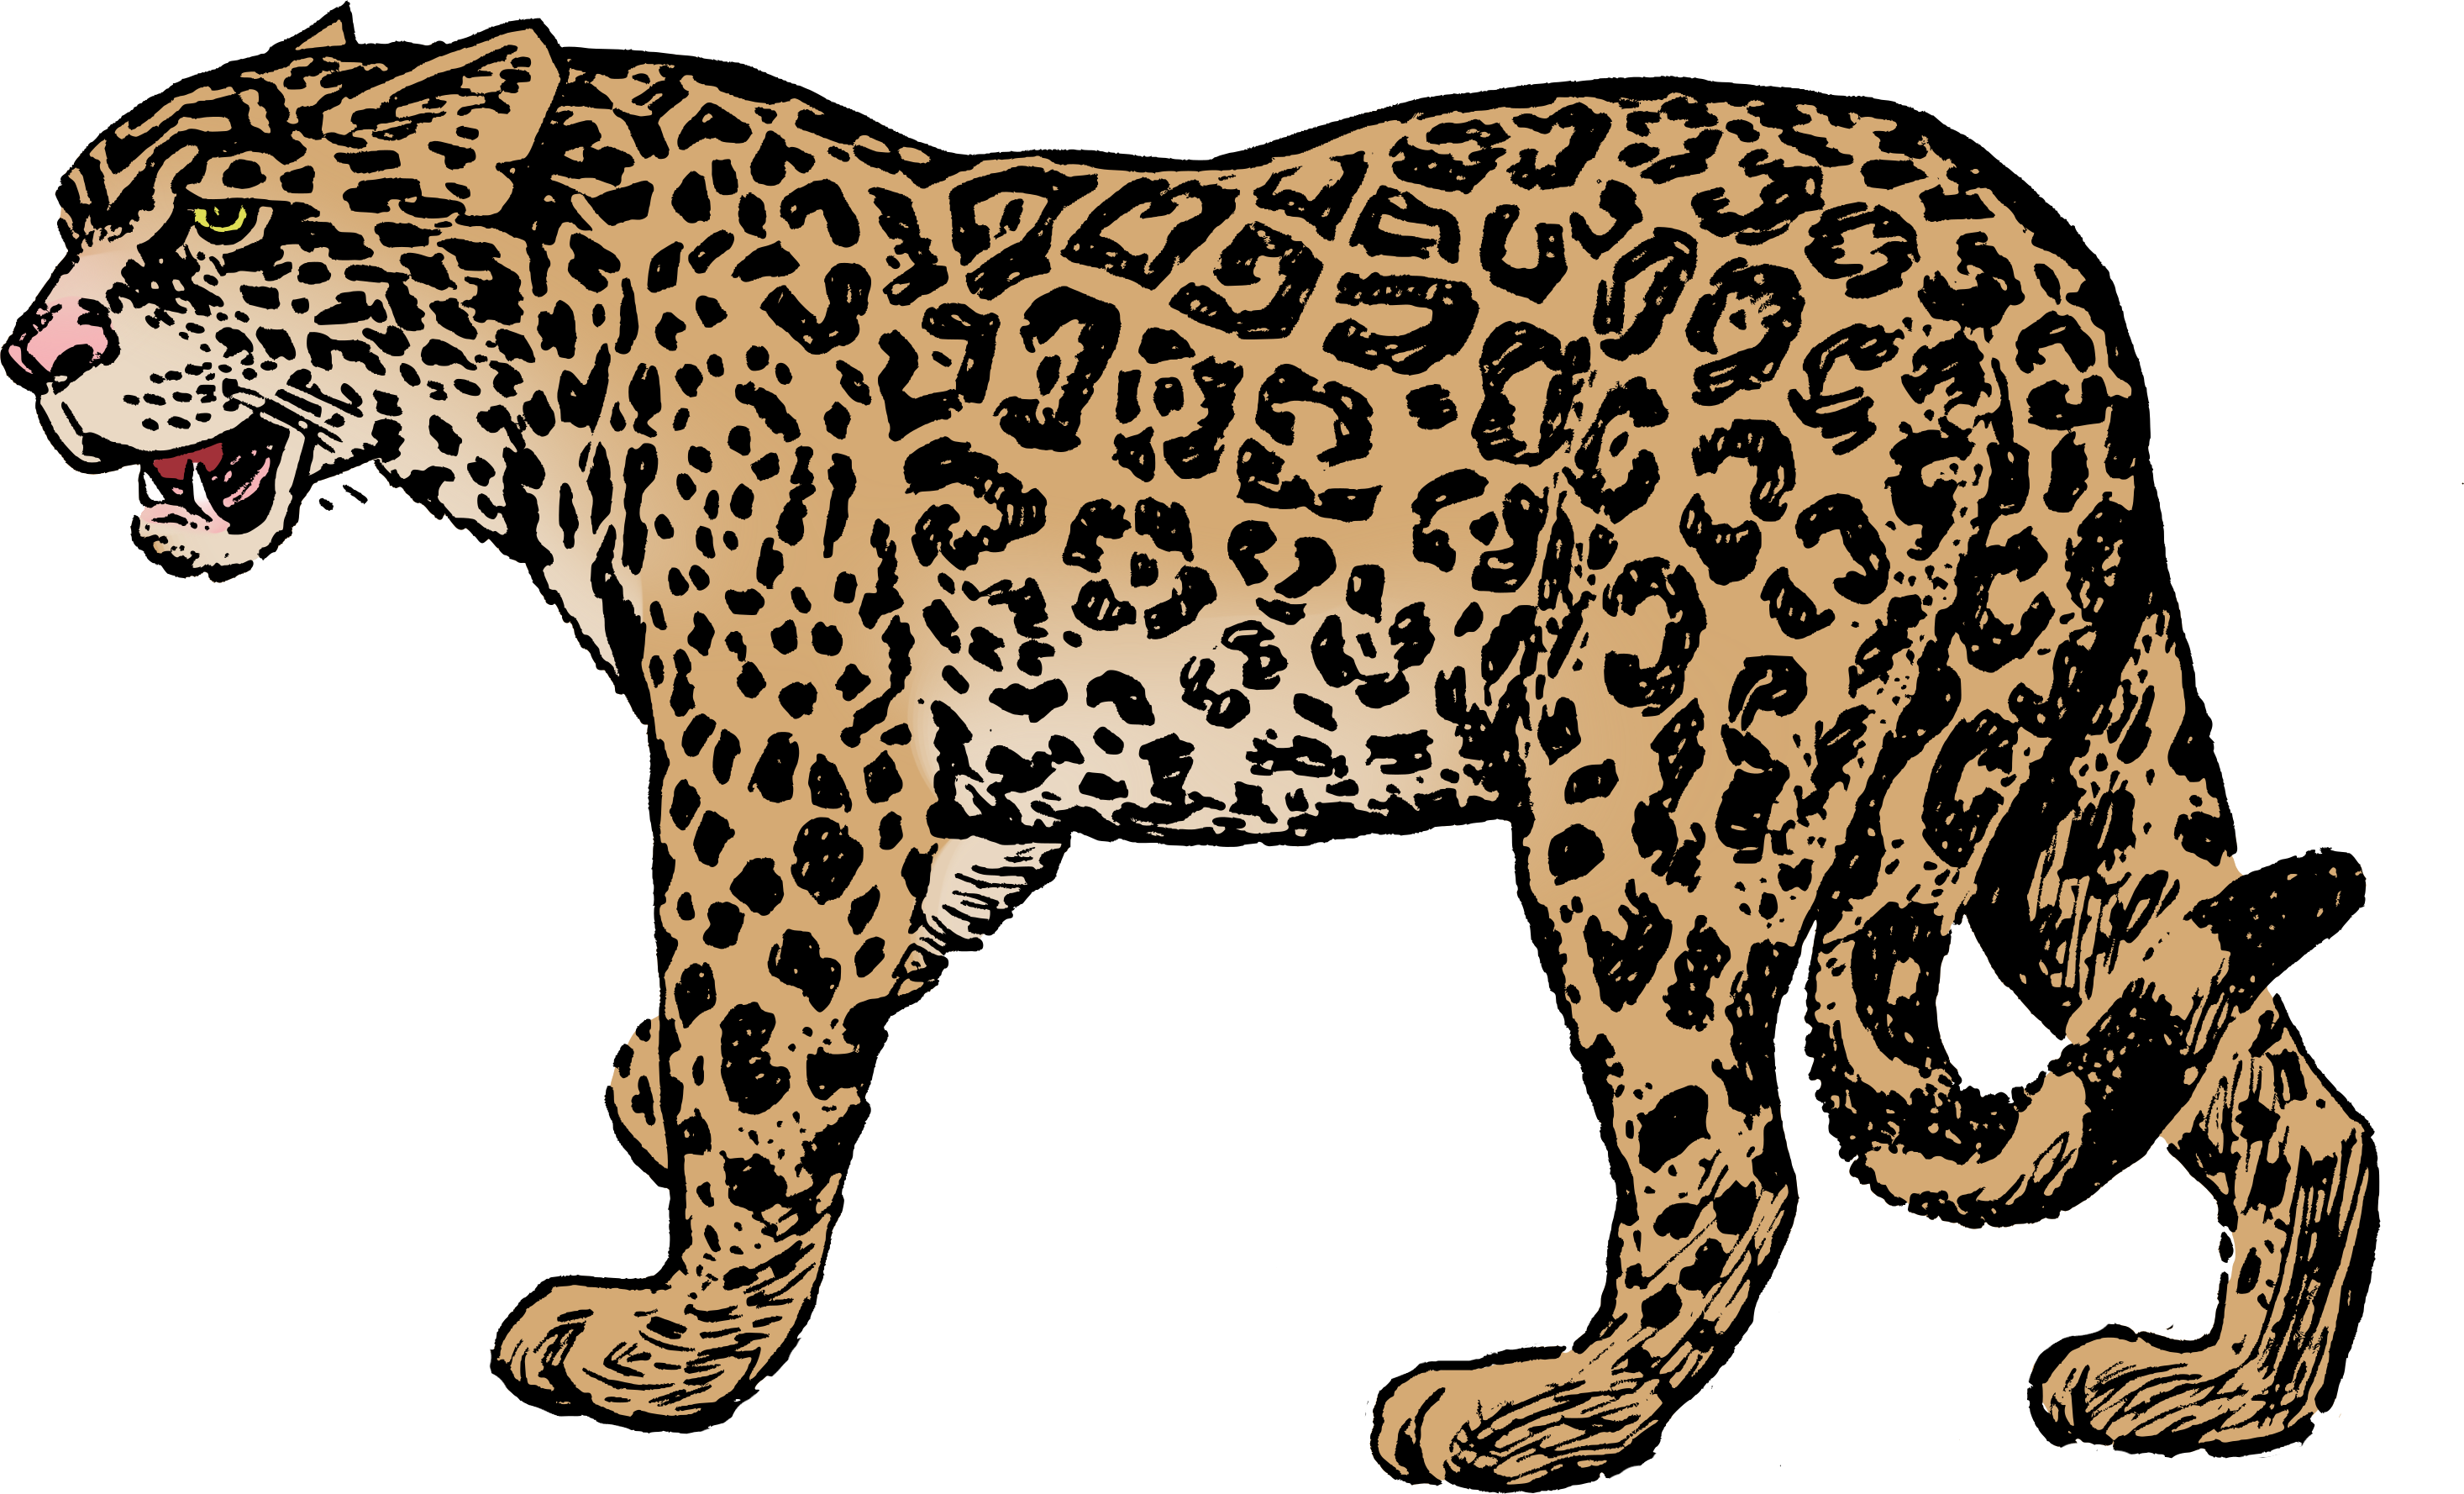
\includegraphics[width=\columnwidth]{Monsters/Animals/Cat, Jaguar}

\subsection{Cat, Lion}\index[monsters]{Lion}
\monsterimage{Monsters/Animals/Cat, Lion}{\statblock{\textbf{Size:} Large

\textbf{Type:} Animal

\textbf{Habitat:} Clear, Desert (Common)

\textbf{Wandering Group:} 1d4 (U)

\textbf{Lair Group:} 1d8 (Nil)

\textbf{Move:} 50 ft.

\textbf{Armor Class:} 6

\textbf{Hit Dice:} 5 (23 HP)

\textbf{Attacks:} 2x Claw (1d4+1) 

\& Bite (1d10)

\textbf{Special:} None

\textbf{Save:} F3

\textbf{Alignment:} None

\textbf{Intelligence:} 2

\textbf{Morale:} 9

\textbf{XP Value:} 175}}

Lions are cats that live in small family groups called prides.

Male lions have a distinctive mane, and are relatively inactive. Although they are very territorial towards other male lions, they will often ignore non-lion creatures unless threatened.

Female lions are active hunters, and work well together. Some will lie in ambush while others chase potential prey towards them.

\subsection{Cat, Mountain Lion}\index[monsters]{Mountain Lion}
\monsterimage{Monsters/Animals/Cat, Mountain Lion}{\statblock{\textbf{Size:} Medium

\textbf{Type:} Animal

\textbf{Habitat:} Desert, Mountains, Underground, Woods (Common)

\textbf{Wandering Group:} 1 (U)

\textbf{Lair Group:} 1d4 (Nil)

\textbf{Move:} 50 ft.

\textbf{Armor Class:} 6

\textbf{Hit Dice:} 3+2 (16 HP)

\textbf{Attacks:} 2x Claw (1d3) \& Bite (1d6)

\textbf{Special:} None

\textbf{Save:} F2

\textbf{Alignment:} None

\textbf{Intelligence:} 2

\textbf{Morale:} 8

\textbf{XP Value:} 50}}

Mountain lions, also known as pumas or cougars, are smaller and less muscled than their plains dwelling cousins.

Mountain lions hunt alone, and will aggressively attack human-sized creatures only if cornered or starving. However, they are inquisitive creatures who love to explore (including cave systems) and are easily attracted to camp sites by the smell of cooking food.

Mountain lions are often trained by dwarves and fulfill the roles that guard and hunting dogs fill for humanoid species that live in lowlands.

\subsection{Cat, Panther}\index[monsters]{Panther}
\statblock{\textbf{Size:} Medium

\textbf{Type:} Animal

\textbf{Habitat:} Clear, Jungle, Woods (Common)

\textbf{Wandering Group:} 1d2 (U)

\textbf{Lair Group:} 1d6 (Nil)

\textbf{Move:} 70 ft.

\textbf{Armor Class:} 4

\textbf{Hit Dice:} 4 (18 HP)

\textbf{Attacks:} 2x Claw (1d4) \& Bite (1d8)

\textbf{Special:} None

\textbf{Save:} F2

\textbf{Alignment:} None

\textbf{Intelligence:} 2

\textbf{Morale:} 8

\textbf{XP Value:} 75}

Panthers are dark furred cats. They are agile, quick and lithe, and are excellent climbers. A favorite hunting strategy is to hide in a tree and leap down knocking prey to the ground.

Panthers hunt either alone or as a mated pair.

Unlike many other cats, they are also strong swimmers, and will readily chase prey into water.

\subsection{Cat, Tiger, Saber-Tooth}\index[monsters]{Saber-Tooth Tiger}\label{monster:Saber-Tooth Tiger}
\statblock{\textbf{Size:} Large

\textbf{Type:} Animal

\textbf{Habitat:} Clear (Very Rare)

\textbf{Wandering Group:} 1d4 (V)

\textbf{Lair Group:} 1d4 (Nil)

\textbf{Move:} 50 ft.

\textbf{Armor Class:} 6

\textbf{Hit Dice:} 8 (36 HP)

\textbf{Attacks:} 2x Claw (1d8) \& Bite (2d8)

\textbf{Special:} None

\textbf{Save:} F4

\textbf{Alignment:} None

\textbf{Intelligence:} 2

\textbf{Morale:} 10

\textbf{XP Value:} 650}

Saber-tooth tigers have over-sized canine teeth, which give them their name. These fangs are present in both sexes, and are used for hunting.

Saber-tooth tigers are built for strength rather than speed, and their usual hunting tactic is to stalk their prey and leap at it from ambush. They will not usually bother to chase fleeing prey unless it is obviously injured or weak.

\subsection{Cat, Tiger}\index[monsters]{Tiger}
\statblock{\textbf{Size:} Large

\textbf{Type:} Animal

\textbf{Habitat:} Woods (Common)

\textbf{Wandering Group:} 1 (U)

\textbf{Lair Group:} 1d3 (Nil)

\textbf{Move:} 50 ft.

\textbf{Armor Class:} 6

\textbf{Hit Dice:} 6 (27 HP)

\textbf{Attacks:} 2x Claw (1d6) \& Bite (2d6)

\textbf{Special:} Camouflage

\textbf{Save: F3}

\textbf{Alignment:} None

\textbf{Intelligence:} 2

\textbf{Morale:} 9

\textbf{XP Value:} 275}

Tigers are heavily built cats. They are easily recognized for their distinctive orange and black striped markings.

Unlike other cats, tigers are keen swimmers.

\textbf{Camouflage:} The tiger's markings provide remarkably effective camouflage in wooded surroundings, causing the tiger to surprise their opponents on a 1-4 on 1d6.

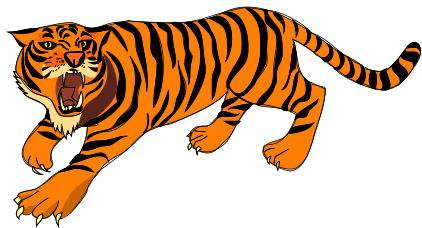
\includegraphics[width=\columnwidth]{Monsters/Animals/Cat, Tiger}

\subsection{Catoblepas}\index[monsters]{Catoblepas}
\statblock{\textbf{Size:} Large

\textbf{Type:} Monster

\textbf{Habitat:} Swamp (Very Rare)

\textbf{Wandering Group:} 0 (Nil)

\textbf{Lair Group:} 1d3 (C)

\textbf{Move:} 20 ft.

\textbf{Armor Class:} 7*

\textbf{Hit Dice:} 7** (32 HP)

\textbf{Attacks:} Tail (1d6) \& Gaze (Special)

\textbf{Special:} Immunity (Death Ray, Energy Drain, 

Instant Death, Poison)

\textbf{Save:} F4

\textbf{Alignment:} None

\textbf{Intelligence:} 2

\textbf{Morale:} 8

\textbf{XP Value:} 1,250}

A catoblepas is a horrible beast with a long neck and tail. Its head is boar shaped, although its tusks are small and not useful in combat.

Catoblepes are generally peaceful creatures that live in swamps and eat all kinds of poisonous plants. They are slow moving and rather ungainly, and would rather simply be left alone than seek out fights; but if threatened they will attack in self defense by lashing with their long tails.

\textbf{Petrifying Gaze:} Anyone who a catoblepas gazes at must make a saving throw vs. death ray or be slain instantly. Unlike the gaze of a basilisk or medusa, it doesn’t matter whether the victim has their eyes closed or is facing away from the catoblepas—it is the catoblepas gazing at the victim that causes the death, not the other way around.

Luckily for most victims, the catoblepas’ heavy head and weak neck mean that it only has a 1 in 4 chance per round of being able to successfully gaze at a single target. However, if a catoblepas gains surprise in combat, then it will always have the opportunity to use its gaze during the surprise round.

Catoblepes are immune to the gaze attacks of other catoblepes.

\subsection{Centaur}\index[monsters]{Centaur}
\statblock{\textbf{Size:} Large

\textbf{Type:} Monster

\textbf{Habitat:} Clear, Woods (Common)

\textbf{Wandering Group:} 1 (Nil)

\textbf{Lair Group:} 2d10 (A)

\textbf{Move:} 60 ft.

\textbf{Armor Class:} 5

\textbf{Hit Dice:} 4* (18 HP)

\textbf{Attacks:} 2x Hoof (1d6) or Weapon (By weapon)

\textbf{Special:} None

\textbf{Save:} F4

\textbf{Alignment:} Neutral

\textbf{Intelligence:} 10

\textbf{Morale:} 8

\textbf{XP Value:} 125}

Centaurs have the body and legs of a horse, with a human torso (plus head and arms) rising up where the neck would be. They are as intelligent as normal humans, and primarily live in woods and forests.

A clan of centaurs will often ally with elves or with human druids, although they can produce spellcasters of their own.

Centaurs will occasionally trade with human villages outside of their woods, but are very reluctant to allow humans to encroach on what they see as their lands.

\subsubsection{Spellcasting}
Centaurs can reach \nth{8} level as either shamans or sorcerers.

\subsubsection{As a Class}\index[classes]{Centaur}
Centaurs can be used as a class using the following statistics:

\statblock{\textbf{Ability Requirements:} Strength 9

\textbf{Prime Requisite:} Strength

\textbf{Ability Modifiers:} Dexterity -2, Constitution +1, Wisdom +1

\textbf{Weapons:} Any

\textbf{Armor:} Any (-1 AC bonus, 30x cost, 3x Encumbrance)

\textbf{Natural AC:} 8 (Immature), 7 (Mature)

\textbf{Special Abilities:} None

\textbf{Magic Item Use:} Fighter}

\begin {table}[H]
  \caption{Centaur Progression}
  \begin{tabularx}{\columnwidth}{>{\bfseries}YYY}
	\thead{Level} & \thead{Experience} & \thead{Hit Dice}\\
	-1 & -4,000 & 2d8\\
	0 & 0 & 4d8\\
	1 & 4,000 & -\\
	2 & 12,000 & 5d8\\
	3 & 28,000 & 6d8\\
	4 & 60,000 & -\\
	5 & 124,000 & 7d8\\
	6 & 250,000 & 8d8\\
	7 & 500,000 & -\\
	8 & 800,000 & 9d8\\
	9 & 1,100,000 & 10d8\\
	10+ & +300,000 & +2 HP
  \end {tabularx}
\end {table}

\subsection{Centipede, Giant}\index[monsters]{Giant Centipede}
\statblock{\textbf{Size:} Small

\textbf{Type:} Animal

\textbf{Habitat:} Clear, Underground, Woods (Common)

\textbf{Wandering Group:} 2d4 (Nil)

\textbf{Lair Group:} 1d8 (Nil)

\textbf{Move:} 20 ft.

\textbf{Armor Class:} 9

\textbf{Hit Dice:} 1/2* (3 HP)

\textbf{Attacks:} Bite (Special)

\textbf{Special:} Poison

\textbf{Save:} F0

\textbf{Alignment:} None

\textbf{Intelligence:} 0

\textbf{Morale:} 7

\textbf{XP Value:} 6}

Giant centipedes are larger cousins of normal centipedes. They have a segmented body with many pairs of legs, and a pair of large mandibles with which they can deliver a poisonous bite.

Giant centipedes normally hide in crevices or rotten wood and wait for small animals to come within reach; then they lunge and deliver a poisonous bite to the intruding animal.

\textbf{Poison:} Although giant centipede poison is strong enough to kill a rat or similar sized creature, it will not kill a person. However, it will cause sickness.

Anyone bitten by a giant centipede must make a saving throw vs. poison or be sickened for 10 days, during which time they can only move at half normal speed and can not perform any other action.

\subsection{Chimera}\index[monsters]{Chimera}
\statblock{\textbf{Size:} Large

\textbf{Type:} Dragon

\textbf{Habitat:} Hills, Mountains, Underground (Very Rare)

\textbf{Wandering Group:} 1d2 (Nil)

\textbf{Lair Group:} 1d4 (F)

\textbf{Move:} 40 ft., 60 ft. (Fly)

\textbf{Armor Class:} 4

\textbf{Hit Dice:} 9** (41 HP)

\textbf{Attacks:} 2x Claw (1d3) \& Butt (2d4) \& 

Bite (1d10) \& Bite (3d4) \& Breath (3d6)

\textbf{Special:} Fire Breath

\textbf{Save:} F9

\textbf{Alignment:} Chaotic

\textbf{Intelligence:} 6

\textbf{Morale:} 9

\textbf{XP Value:} 2,300}

A chimera, as the name implies, appears to be a strange combination of other beasts.

Chimerae have the rear body of a goat, the front body of a lion, the wings and tail of a dragon, and three heads—goat, lion and dragon.

Although sapient, chimerae are not terribly smart, and can often be tricked or bullied into working for a more powerful creature.

Chimerae are extremely territorial, and will aggressively chase intruders away from their lair.

\textbf{Fire Breath:} The dragon head of a chimera is capable of breathing fire three times per day in a cone 50 feet long and 10 feet wide at the end.

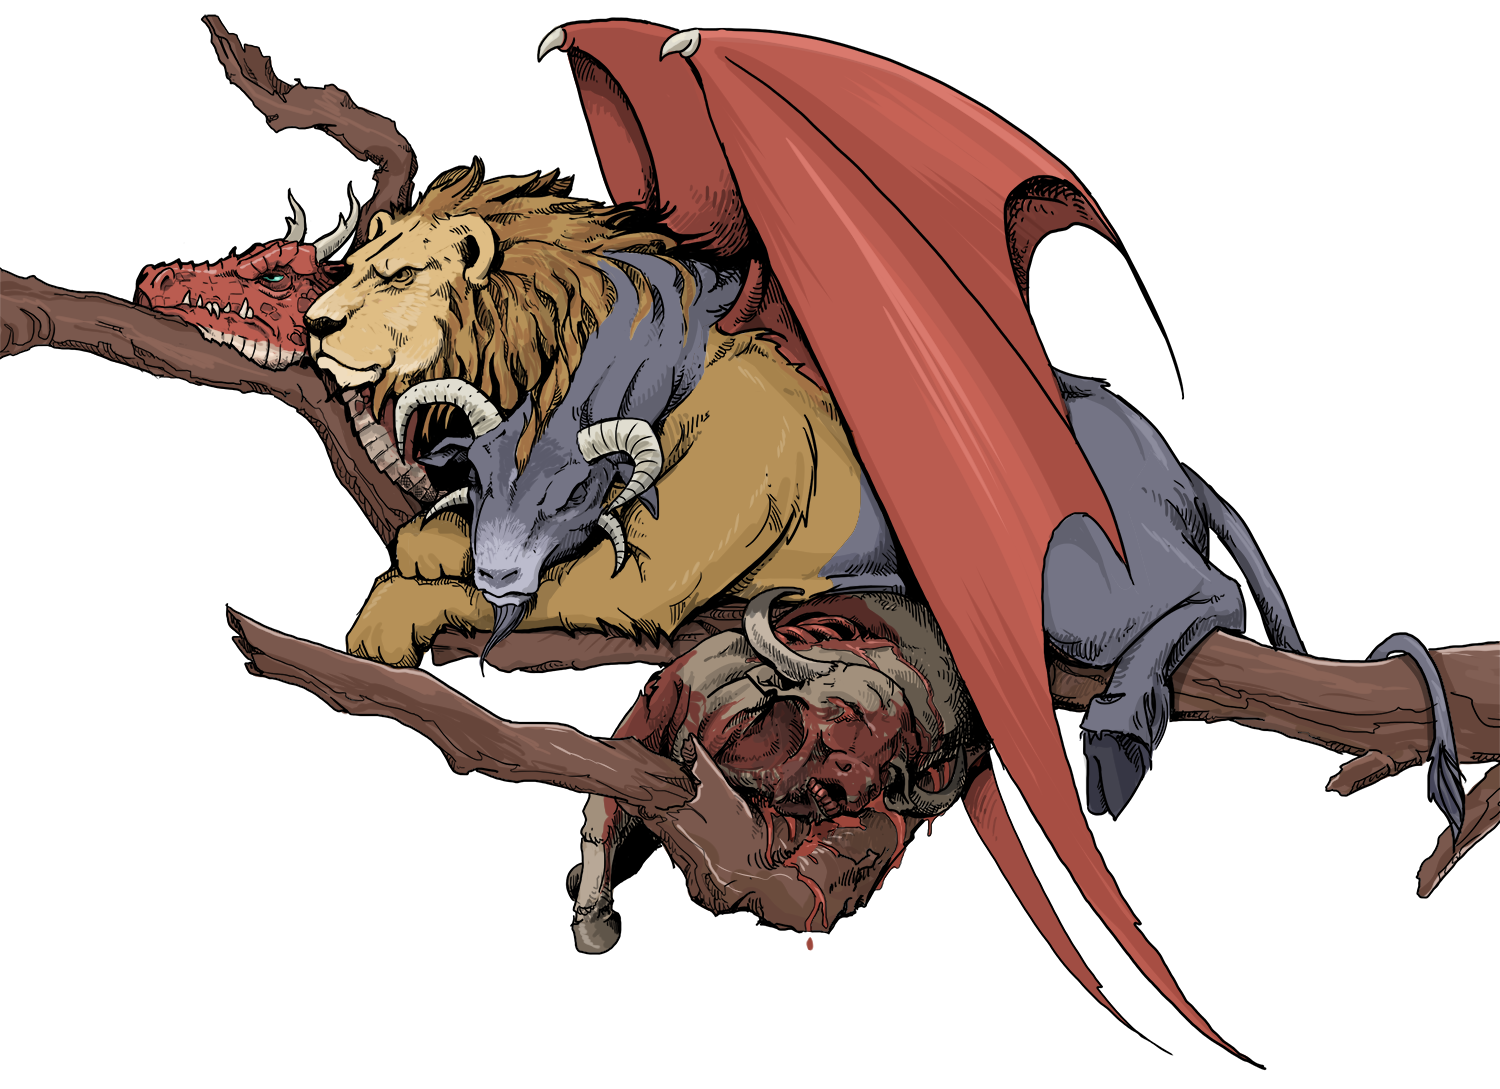
\includegraphics[width=\columnwidth]{Monsters/Chimera}

\subsection{Cockatrice}\index[monsters]{Cockatrice}
\begin {table}[H]
	\normalsize
  \begin{tabularx}{\columnwidth}{@{}>{\bfseries}XXX@{}}
	\hiderowcolors
	& \textbf{Prime Plane} & \textbf{Home Plane}\\
	Size: & Small & Small\\
	Type: & Extraplanar, Monster & Monster\\
	Habitat: & Any (Very Rare) & Elemental Plane of Earth (Very Rare)\\
	Wandering Group: & 1d4 (Nil) & 1d20 (Nil)\\
	Lair Group: & 2d4 (D) & 2d20 (D)\\
	Move: & 30 ft., 60 ft. (Fly) & 40 ft., 80 ft. (Fly)\\
	Armor Class: & 6 & 6\\
	Hit Dice: & 5** (23 HP) & 1+1 (6 HP)\\
	Attacks: & Beak (1d6) & Beak (1 hit point)\\
	Special: & Petrification & Petrification\\
	Save: & F5 & F1\\
	Alignment: & None & None\\
	Intelligence: & 2 & 2\\
	Morale: & 7 & 7\\
	XP Value: & 425 & 15\\
	\showrowcolors
  \end {tabularx}
\end {table}

A cockatrice is a magical creature that looks like a drab gray cockerel with a snake’s tail.

A cockatrice is normally peaceful, and is content to scavenge bits of detritus and plant material and be left alone.

\textbf{Petrification:} Any living (non-plant) creature that touches or is touched by a cockatrice must make a saving throw vs. petrification or be turned to stone.

Creatures attacking the cockatrice using natural weapons (including adventurers using unarmed attacks) must make a saving throw each time they hit, and anyone successfully hit by the cockatrice’s attack must also make a saving throw.

\subsubsection{Home Plane}
Cockatrices originate from the Elemental Plane of Earth. When on that plane they appear as foot-long bird-like creatures composed of soft earth.

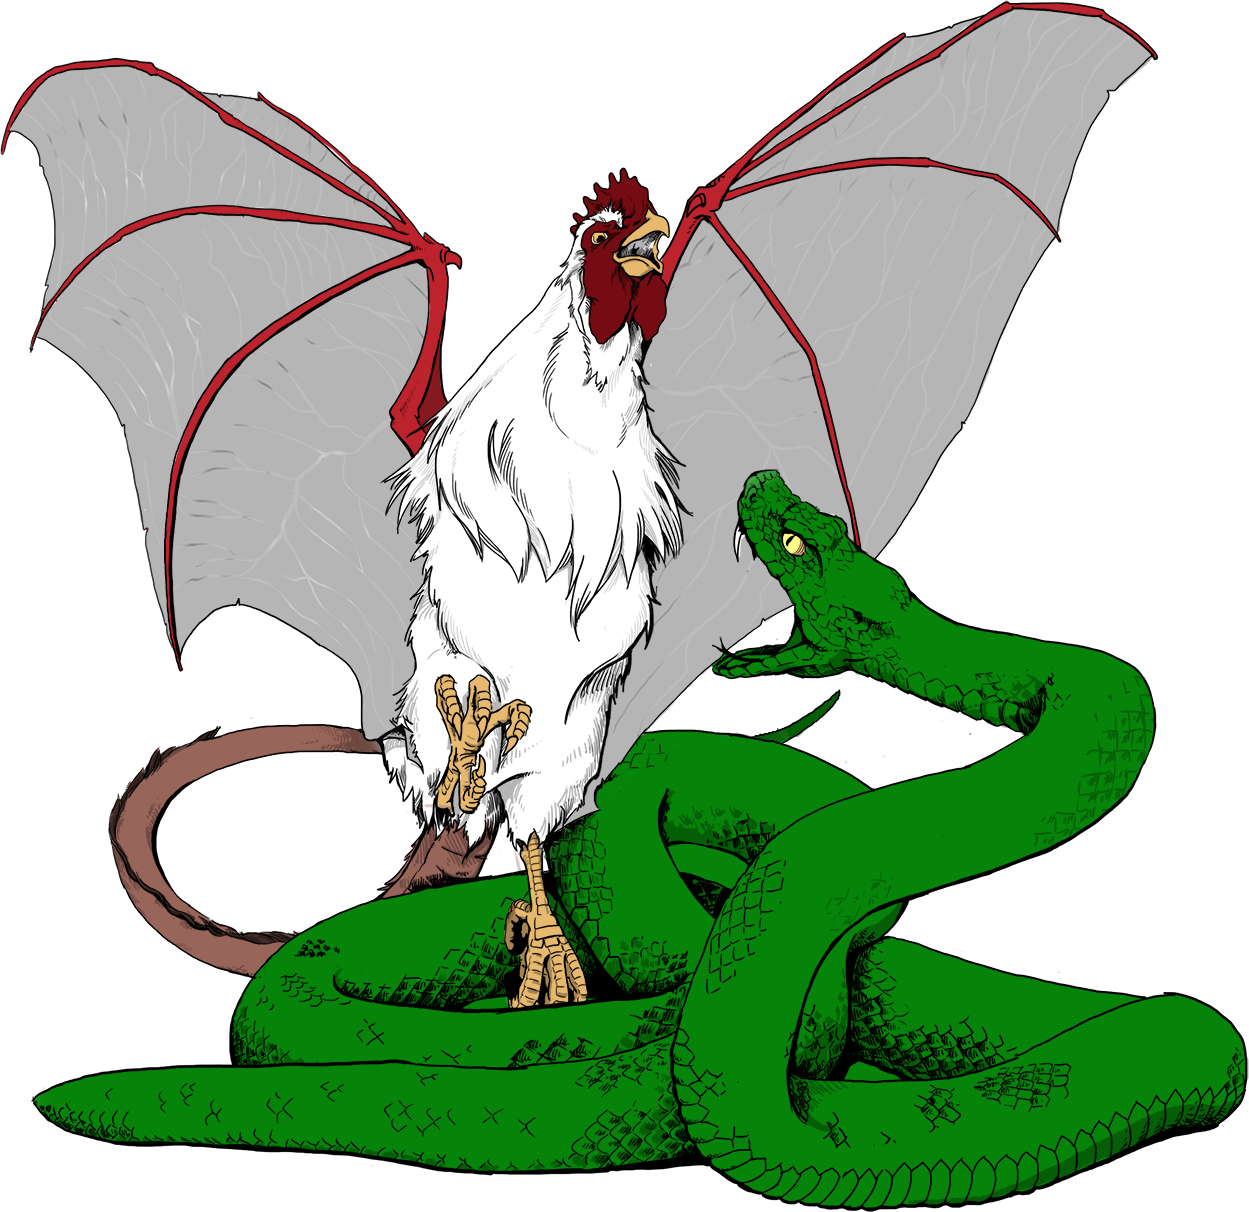
\includegraphics[width=\columnwidth]{Monsters/Cockatrice}

\subsection{Coerl}\index[monsters]{Coerl}
\statblock{\textbf{Size:} Large

\textbf{Type:} Monster

\textbf{Habitat:} Hills, Jungle, Woods (Rare)

\textbf{Wandering Group:} 1d4 (Nil)

\textbf{Lair Group:} 1d4 (D)

\textbf{Move:} 50 ft.

\textbf{Armor Class:} 4

\textbf{Hit Dice:} 6* (27 HP)

\textbf{Attacks:} 2x Tentacle (2d4) or Bite (1d6)

\textbf{Special:} Displacement, Ferocious Bite

\textbf{Save:} F6

\textbf{Alignment:} None

\textbf{Intelligence:} 3

\textbf{Morale:} 8

\textbf{XP Value:} 500}

Coerls are large black panther-like creatures with six legs and a pair of tentacles protruding out of their shoulder.

For some reason, coerls hate Blink Dogs and attack them on sight.

\textbf{Displacement:} The skin of a coerl bends light rays, causing the coerl to appear 3 ft. from it's actual position. Attackers suffer a -2 penalty to their to-hit roll and the coerl gains a +2 bonus to all their saving throws.

With a successful attack roll with a +2 bonus, a coerl can bite a target who has 6 hit points or less for 1d6+2 damage.

\textbf{Ferocious Bite:} When using their bite attack against a target that has 6 hit points or less remaining, the coerl gains a +2 bonus to their attack and damage roll.

\subsection{Crab, Giant}\index[monsters]{Giant Crab}
\monsterimage{Monsters/Animals/Crab, Giant}{\statblock{\textbf{Size:} Medium

\textbf{Type:} Animal

\textbf{Habitat:} Ocean, River (Rare)

\textbf{Wandering Group:} 1d2 (Nil)

\textbf{Lair Group:} 1d6 (Nil)

\textbf{Move:} 20 ft.

\textbf{Armor Class:} 2

\textbf{Hit Dice:} 3 (14 HP)

\textbf{Attacks:} 2x Claw (2d6)

\textbf{Special:} None

\textbf{Save:} F2

\textbf{Alignment:} None

\textbf{Intelligence:} 2

\textbf{Morale:} 7

\textbf{XP Value:} 35}}

Giant crabs are larger versions of normal crabs.

Unlike normal crabs, giant crabs are actively carnivorous and will attack most things smaller than them that they encounter.

Giant crabs are normally aquatic, but can survive on land for up to half an hour before having to return to the water.

Giant crabs do not swim but walk along the bottom of the water.

\subsection{Crocodile}\index[monsters]{Crocodile}
\monsterimage{Monsters/Animals/Crocodile}{\statblock{\textbf{Size:} Medium

\textbf{Type:} Animal

\textbf{Habitat:} River, Swamp (Common)

\textbf{Wandering Group:} 0 (Nil)

\textbf{Lair Group:} 1d8 (Nil)

\textbf{Move:} 30 ft., 30 ft. (Swim)

\textbf{Armor Class:} 5

\textbf{Hit Dice:} 2 (9 HP)

\textbf{Attacks:} Bite (1d8)

\textbf{Special:} None

\textbf{Save:} F1

\textbf{Alignment:} None

\textbf{Intelligence:} 2

\textbf{Morale:} 7

\textbf{XP Value:} 20}}

Crocodiles are reptiles that live in water and swamps. They are air breathers, and usually float on the surface with their nostrils exposed.

Crocodiles come onto land to sun themselves, and to lay their eggs, although they are less agile on land and do their hunting in the water, where they are particularly attracted to the smell of blood and by seeing creatures thrash around.

\subsection{Cyclops}\index[monsters]{Cyclops}
\statblock{\textbf{Size:} Large

\textbf{Type:} Giant

\textbf{Habitat:} Hills, Mountains (Rare)

\textbf{Wandering Group:} 1 (Nil)

\textbf{Lair Group:} 1d4 (E + 5,000 gp)

\textbf{Move:} 30 ft.

\textbf{Armor Class:} 5

\textbf{Hit Dice:} 13* (65 HP)

\textbf{Attacks:} Club (3d10)

\textbf{Special:} Rock Throwing

\textbf{Save:} F13

\textbf{Alignment:} Chaotic

\textbf{Intelligence:} 9

\textbf{Morale:} 9

\textbf{XP Value:} 2,300}

A cyclops is a giant with a single eye in the center of its forehead.

Despite their great power, cyclopes are very slow-witted and peaceful creatures who are content to herd goats and sheep and be left alone by others. They are quick to anger, however, and if provoked they are likely to attack with huge clubs (with which they have nothing more than basic mastery) or by throwing rocks.

All attacks by cyclopes take a -2 penalty due to their poor depth perception.

\textbf{Rock Throwing:} Cyclopes can throw rocks with a range of (60/130/200) feet, for 3d6 damage.

\subsubsection{Spellcasting}
Cyclopes can become shamans of up to \nth{4} level, and (incredibly rarely) sorcerers of up to \nth{2} level.

\subsection{Demon}
Demons are incredibly powerful creatures created by \iref[chap:Immortals]{Immortals} from the souls of mortals as agents of chaos and destruction.

\textbf{Immunity to Magic:} All demons are immune to magic cast by mortals and have Anti-Magic of 25\% against magic cast by \iref[chap:Immortals]{Immortals}.

\subsubsection{Balor}\index[monsters]{Balor}
\statblock{\textbf{Size:} Large

\textbf{Type:} Exalted, Extraplanar

\textbf{Habitat:} Any (Very Rare)

\textbf{Wandering Group:} 1 (Nil)

\textbf{Lair Group:} 1d2 (G)

\textbf{Move:} 20 ft., 60 ft. (Fly)

\textbf{Armor Class:} 0*

\textbf{Hit Dice:} 25********** (113 HP)

\textbf{Attacks:} Sword of Slicing (1d10+5) \& 

Whip of Draining (1d2+5)

\textbf{Special:} Immunity (Magic, Weapons < +2), Powers

\textbf{Power Reserve:} 300

\textbf{Save:} I1

\textbf{Alignment:} Chaotic

\textbf{Intelligence:} 30

\textbf{Morale:} 9

\textbf{XP Value:} 33,500}

A balor is a humanoid with a horned head and leathery wings. They always use a two-handed Sword of Slicing +5 (which they can wield in one hand) and a Whip of Draining +5.

Balors are highly charismatic, will rarely attack by surprise even if given the chance, and prefer to see their opponents acknowledge their superiority and surrender without a fight.

\textbf{Powers:} Balors can spend their power points on the Prepare Mortal Magic spell, and have the Call Other, Enhanced Reflexes, Howl, and Summon Weapons powers.

\subsubsection{Glabrezu}\index[monsters]{Glabrezu}
\statblock{\textbf{Size:} Large

\textbf{Type:} Exalted, Extraplanar

\textbf{Habitat:} Any (Very Rare)

\textbf{Wandering Group:} 1 (Nil)

\textbf{Lair Group:} 1d3 (E)

\textbf{Move:} 60 ft., 20 ft. (Fly)

\textbf{Armor Class:} 0*

\textbf{Hit Dice:} 16********** (72 HP)

\textbf{Attacks:} 2x Pincer (2d6) \& 

2x Horn (1d8) \& Bite (1d6)

\textbf{Special:} Immunity (Magic, 

Non-Silver Normal Weapons), Powers

\textbf{Power Reserve:} 200

\textbf{Save:} I1

\textbf{Alignment:} Chaotic

\textbf{Intelligence:} 25

\textbf{Morale:} 9

\textbf{XP Value:} 12,850}

A glabrezu is a humanoid with a horned wolf’s head and two pairs of arms. The lower pair are normal, but the upper pair are over-sized and end in large pincers.

Glabrezu delight in fire magics and burning things. When dealing with mortals, they prefer bribery to outright threats; often giving riches in exchange for service to their (often un-named) patron.

\textbf{Powers:} Glabrezu can spend their power points on the Prepare Mortal Magic spell, and have the Call Other, Control Undead, Enhanced Reflexes, and Howl powers.

\subsubsection{Hezrou}\index[monsters]{Hezrou}
\statblock{\textbf{Size:} Medium

\textbf{Type:} Exalted, Extraplanar

\textbf{Habitat:} Any (Very Rare)

\textbf{Wandering Group:} 1 (Nil)

\textbf{Lair Group:} 1d3

\textbf{Move:} 60 ft., 20 ft. (Fly)

\textbf{Armor Class:} 0

\textbf{Hit Dice:} 13********** (59 HP)

\textbf{Attacks:} 2x Claw (1d3) \& Bite (2d8+2)

\textbf{Special:} Immunity to Magic, Powers

\textbf{Power Reserve:} 100

\textbf{Save:} I1

\textbf{Alignment:} Chaotic

\textbf{Intelligence:} 20

\textbf{Morale:} 9

\textbf{XP Value:} 10,850}

Hezrou are humanoid toads. They prefer to use undead as minions and agents wherever possible, and will usually act through such agents rather than in person where possible.

\textbf{Powers:} Hezrou can spend their power points on the Prepare Mortal Magic spell, and have the Call Other, Control Undead, Enhanced Reflexes, and Snap powers.

\subsubsection{Marilith}\index[monsters]{Marilith}
\statblock{\textbf{Size:} Large

\textbf{Type:} Exalted, Extraplanar

\textbf{Habitat:} Any (Very Rare)

\textbf{Wandering Group:} 1 (Nil)

\textbf{Lair Group:} 1d2 (F)

\textbf{Move:} 40 ft., 50 ft. (Fly)

\textbf{Armor Class:} 0*

\textbf{Hit Dice:} 22********** (99 HP)

\textbf{Attacks:} 6x Weapon (By weapon) \& Tail (2d8)

\textbf{Special:} Immunity (Magic, Normal Weapons), Powers

\textbf{Power Reserve:} 300

\textbf{Save:} I1

\textbf{Alignment:} Chaotic

\textbf{Intelligence:} 28

\textbf{Morale:} 9

\textbf{XP Value:} 25,250}

Mariliths have a six-armed female human body on top of a snake tail.

\textbf{Powers:} Mariliths can spend their power points on the Prepare Mortal Magic spell, and have the Call Other, Control Undead, Enhanced Reflexes, and Spit Poison powers.

Mariliths relish combat more than any other type of demon, and respect those—even enemies—who fight well.

\subsubsection{Nalfeshnee}\index[monsters]{Nalfeshnee}
\statblock{\textbf{Size:} Large

\textbf{Type:} Exalted, Extraplanar

\textbf{Habitat:} Any (Very Rare)

\textbf{Wandering Group:} 1 (Nil)

\textbf{Lair Group:} 1d3 (E)

\textbf{Move:} 30 ft., 40 ft. (Fly)

\textbf{Armor Class:} 0*

\textbf{Hit Dice:} 19********** (86 HP)

\textbf{Attacks:} 2x Claw (1d8) \& Bite (2d4)

\textbf{Special:} Immunity (Magic, Normal Weapons), Powers

\textbf{Power Reserve:} 200

\textbf{Save:} I1

\textbf{Alignment:} Chaotic

\textbf{Intelligence:} 26

\textbf{Morale:} 9

\textbf{XP Value:} 17,750}

A nalfeshnee is a bulky creature with the body and arms of a powerful ape and goat-like legs with hoofed feet. Their heads are like those of boars, but with bat like ears. Nalfeshnee have feathered wings on their back that look ridiculously small for their size.

Nalfeshnee like to give the impression that they are dumb thugs, taking advantage of their brutish appearance to hide their intellect and scheming nature.

\textbf{Powers:} Nalfeshnee can spend their power points on the Prepare Mortal Magic spell, and have the Call Other, Control Undead, Enhanced Reflexes, and Groan powers.

\subsubsection{Succubus}\index[monsters]{Succubus}
\statblock{\textbf{Size:} Medium

\textbf{Type:} Exalted, Extraplanar

\textbf{Habitat:} Any (Very Rare)

\textbf{Wandering Group:} 1 (Nil)

\textbf{Lair Group:} 1 (I x 2)

\textbf{Move:} 40 ft.

\textbf{Armor Class:} 0*

\textbf{Hit Dice:} 10********** (45 HP)

\textbf{Attacks:} None

\textbf{Special:} Immunity (Magic, Weapons < +2), Powers

\textbf{Power Reserve:} 100

\textbf{Save:} I1

\textbf{Alignment:} Chaotic

\textbf{Intelligence:} 12

\textbf{Morale:} 9

\textbf{XP Value:} 8,500}

The least monstrous of the demons, succubi appear to be attractive humans of either sex with wings and vestigial horns.

Succubi are master seducers, and usually charm their way into getting what they want. They avoid combat, relying on their Leech power and on spells if pressed; but would much rather talk their way out of a potential fight.

Because of their great charm and charisma, succubi prefer to handle issues directly rather than rely on agents, and are thus the most commonly encountered type of demon.

\textbf{Powers:} Succubi can spend their power points on the Prepare Mortal Magic spell, and have the Call Other, Control Undead, Enhanced Reflexes, and Leech powers.

\subsubsection{Vrock}\index[monsters]{Vrock}
\statblock{\textbf{Size:} Large

\textbf{Type:} Exalted, Extraplanar

\textbf{Habitat:} Any (Very Rare)

\textbf{Wandering Group:} 1 (Nil)

\textbf{Lair Group:} 1d3 (B)

\textbf{Move:} 40 ft., 60 ft. (Fly)

\textbf{Armor Class:} 0

\textbf{Hit Dice:} 10**********

\textbf{Attacks:} 2x Claw (1d4) \& 

2x Talon (1d8) \& Beak (1d6)

\textbf{Special:} Immunity to Magic, Powers

\textbf{Power Reserve:} 100

\textbf{Save:} I1

\textbf{Alignment:} Chaotic

\textbf{Intelligence:} 16

\textbf{Morale:} 9

\textbf{XP Value:} 8,500}

Vrock are scrawny humanoids with vulture heads, feet and wings.

Vrocks are the least powerful and the least subtle of all the demons. They tend to get bored easily by plotting and scheming and prefer to simply fly around having fun—although since “having fun” includes killing people, this doesn’t make them much less dangerous than other demons.

Other demons often consider vrocks to be a liability for drawing too much attention, but are happy to deploy them when such attention will be a suitable diversion from their real plans.

\textbf{Powers:} Vrocks can spend their power points on the Prepare Mortal Magic spell, and have the Call Other, Control Undead, Enhanced Reflexes, and Swoop powers.

\subsection{Dinosaur}
In game terms, dinosaur means any prehistoric creature.

\textbf{Swallow Whole:} If a large dinosaur hits an opponent with a natural roll of 20 that is human-sized or smaller, they may swallow the opponent. These dinosaurs contain treasure in their stomachs from previously swallowed victims.

\subsubsection{Aquatic Dinosaur}\index[monsters]{Aquatic Dinosaur}
\begin {table}[H]
	\normalsize
  \begin{tabularx}{\columnwidth}{@{}>{\bfseries}XXXX@{}}
	\hiderowcolors
	& \textbf{Small} & \textbf{Large} & \textbf{Armored}\\
	Size: & Small-Medium & Large & Large\\
	Type: & Animal & Animal & Animal\\
	Habitat: & River, & River, & River, \\
	& Ocean (Rare) & Ocean (Rare) & Ocean (Rare)\\
	Wandering Group: & 1d2 (Nil) & 1 (U+V) & 1 (Nil)\\
	Lair Group: & 2d8 (Nil) & 1d4 (Nil) & 1d4 (Nil)\\
	Move: & 5 ft., & 10 ft., & 5 ft., \\
	& 30 ft. (Swim) & 40 ft. (Swim) & 20 ft. (Swim)\\
	Armor Class: & 7 & 6 & 3\\
	Hit Dice: & 4 (18 HP) & 16 (72 HP) & 7 (32 HP)\\
	Attacks: & Bite (1d6) & Bite (3d6) & Bite (1d8)\\
	Special: & None & Swallow Whole & None\\
	Save: & F1 & F8 & F3\\
	Alignment: & None & None & None\\
	Intelligence: & 2 & 2 & 2\\
	Morale: & 7 & 9 & 8\\
	XP Value: & 75 & 2,000 & 550\\
	\showrowcolors
  \end {tabularx}
\end {table}

Aquatic dinosaurs are large omnivorous water-dwelling creatures. They come in two size ranges, with small being creatures such as an ichthyosaur and large being creatures such as a plesiosaur or mosasaur. There is also an armored variety, which is protected by a large shell. These are creatures such as an archelon.

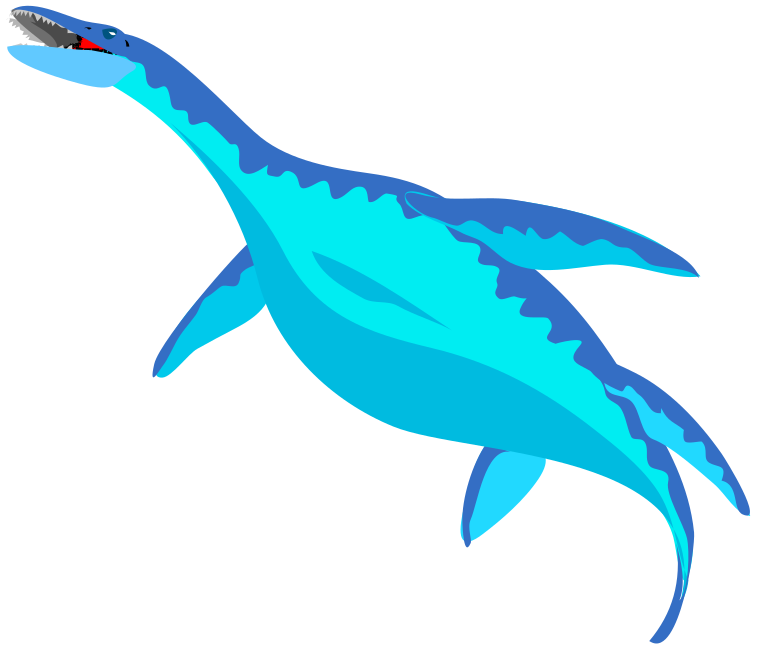
\includegraphics[width=\columnwidth]{Monsters/Animals/Dinosaur, Aquatic}

\subsubsection{Carnivorous Dinosaur}\index[monsters]{Carnivorous Dinosaur}
\begin {table}[H]
	\normalsize
  \begin{tabularx}{\columnwidth}{@{}>{\bfseries}XXXX@{}}
	\hiderowcolors
	& \textbf{Small} & \textbf{Large}\\
	Size: & Small-Medium & Large\\
	Type: & Animal & Animal\\
	Habitat: & Any except Arctic (Rare) & Any except Arctic (Rare)\\
	Wandering Group: & 2d4 (Nil) & 1 (U+V)\\
	Lair Group: & 2d6 (Nil) & 1d2 (Nil)\\
	Move: & 40 ft. & 50 ft.\\
	Armor Class: & 5 & 4\\
	Hit Dice: & 3 (14 HP) & 20 (90 HP)\\
	Attacks: & 2x Claw (1 point) \& Bite (1d8) & 2x Claw (2d6) \& Bite (5d8)\\
	Special: & None & Swallow Whole\\
	Save: & F3 & F9\\
	Alignment: & None & None\\
	Intelligence: & 4 & 2\\
	Morale: & 9 & 9\\
	XP Value: & 35 & 2,375\\
	\showrowcolors
  \end {tabularx}
\end {table}

Carnivorous dinosaurs are large meat-eating creatures. They come in two size ranges, with small being creatures such as a deinonychus or dimetrodon and large being creatures such as a tyrannosaur or a spinosaur.

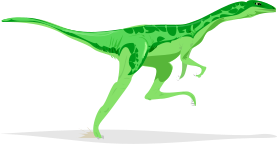
\includegraphics[width=\columnwidth]{Monsters/Animals/Dinosaur, Carnivorous}

\subsubsection{Herbivorous Dinosaur}\index[monsters]{Herbivorous Dinosaur}
\begin {table}[H]
	\normalsize
  \begin{tabularx}{\columnwidth}{@{}>{\bfseries}XXX@{}}
	\hiderowcolors
	& \textbf{Small} & \textbf{Large}\\
	Size: & Small-Medium & Large\\
	Type: & Animal & Animal\\
	Habitat: & Any except Arctic (Rare) & Any except Arctic (Rare)\\
	Wandering Group: & 2d6 (Nil) & 2d6 (Nil)\\
	Lair Group: & 3d10 (Nil) & 3d10 (Nil)\\
	Move: & 40 ft. & 20 ft.\\
	Armor Class: & 7 & 5\\
	Hit Dice: & 4 (18 HP) & 25 (113 HP)\\
	Attacks: & Horn (2d4) & Tail (2d8) or\\
	& & Trample (4d8)\\
	Special: & None & Trample,\\
	& & Swallow Whole\\
	Save: & F1 & F13\\
	Alignment: & None & None\\
	Intelligence: & 2 & 2\\
	Morale: & 9 & 7\\
	XP Value: & 75 & 3,500\\
	\showrowcolors
  \end {tabularx}
\end {table}

Herbivorous dinosaurs are large plant-eating creatures. They come in two size ranges, with small being creatures such as a triceratops or ankylosaur and large being creatures such as a triceratops or ankylosaur.

\textbf{Trample:} Large herbivorous dinosaurs can trample over anything smaller than itself that gets in its way. Any such victim suffers 4d8 points of damage. The trample is treated as if doing the Charge action.

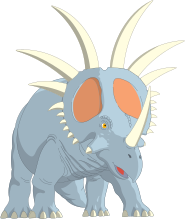
\includegraphics[width=\columnwidth]{Monsters/Animals/Dinosaur, Herbivore}

\subsection{Djinni}\index[monsters]{Djinni}
\begin {table}[H]
	\normalsize
  \begin{tabularx}{\columnwidth}{>{\bfseries}XXX}
	\hiderowcolors
	& \textbf{Prime Plane} & \textbf{Home Plane}\\
	Size: & Medium & Medium\\
	Type: & Extraplanar, Monster & Monster\\
	Habitat: & Desert (Rare) & Elemental Plane of Air (Rare)\\
	Wandering Group: & 1 (Nil) & 1d4 (Nil)\\
	Lair Group: & 1 (Nil) & 1d100 (Nil)\\
	Move: & 30 ft., 80 ft. (Fly) & 30 ft., 80 ft. (Fly)\\
	Armor Class: & 5* & 3*\\
	Hit Dice: & 7+1* (33 HP) & 7+1* (33 HP)\\
	Attacks: & Fist (2d8) & Fist (2d8)\\
	Special: & Immunity to Normal Weapons, Spell-like Abilities, Whirlwind & Detect Invisible, Immunity (\nth{1} level Spells, Normal Weapons, Water), Spell-like Abilities, Whirlwind\\
	Save: & F14 & F14\\
	Alignment: & Chaotic & Chaotic\\
	Intelligence: & 14 & 14\\
	Morale: & 12 & 9\\
	XP Value: & 1,025 & 1,025\\
	\showrowcolors
  \end {tabularx}
\end {table}

Djinn are magical desert dwelling spirits. They appear as blue skinned humans. Despite being creatures of chaos, djinn are normally good-natured and friendly.

\textbf{Spell-like Abilities:} A djinni can cast the following spells 3 times a day (as a \nth{7} level caster if appropriate): \iref[spell:Create Food]{Create Food}, \iref[spell:Woodform]{Woodform} or \iref[spell:Clothform]{Clothform}, \iref[spell:Stoneform]{Stoneform} or \iref[spell:Ironform]{Ironform}, \iref[spell:Invisibility]{Invisibility}, and \iref[spell:Phantasmal Force]{Phantasmal Force}.

\textbf{Whirlwind:} A djinni can transform over the course of five rounds into a whirlwind 70 feet tall and 10 feet in diameter at the base. While in this form, the pasha can move at a rate of 40 feet, and any creature it engulfs takes 2d6 damage. Creatures of less than 2 hit dice must make a saving throw vs. death ray or be swept aside.

\subsubsection{Home Plane}
Djinni originate from the Elemental Plane of Air.

\textbf{Detect Invisibility:} Djinni can see invisible creatures within 120 feet.

\subsubsection{Spellcasting}
Djinni can be shamans (to \nth{4} level) or sorcerers (to \nth{6} level).

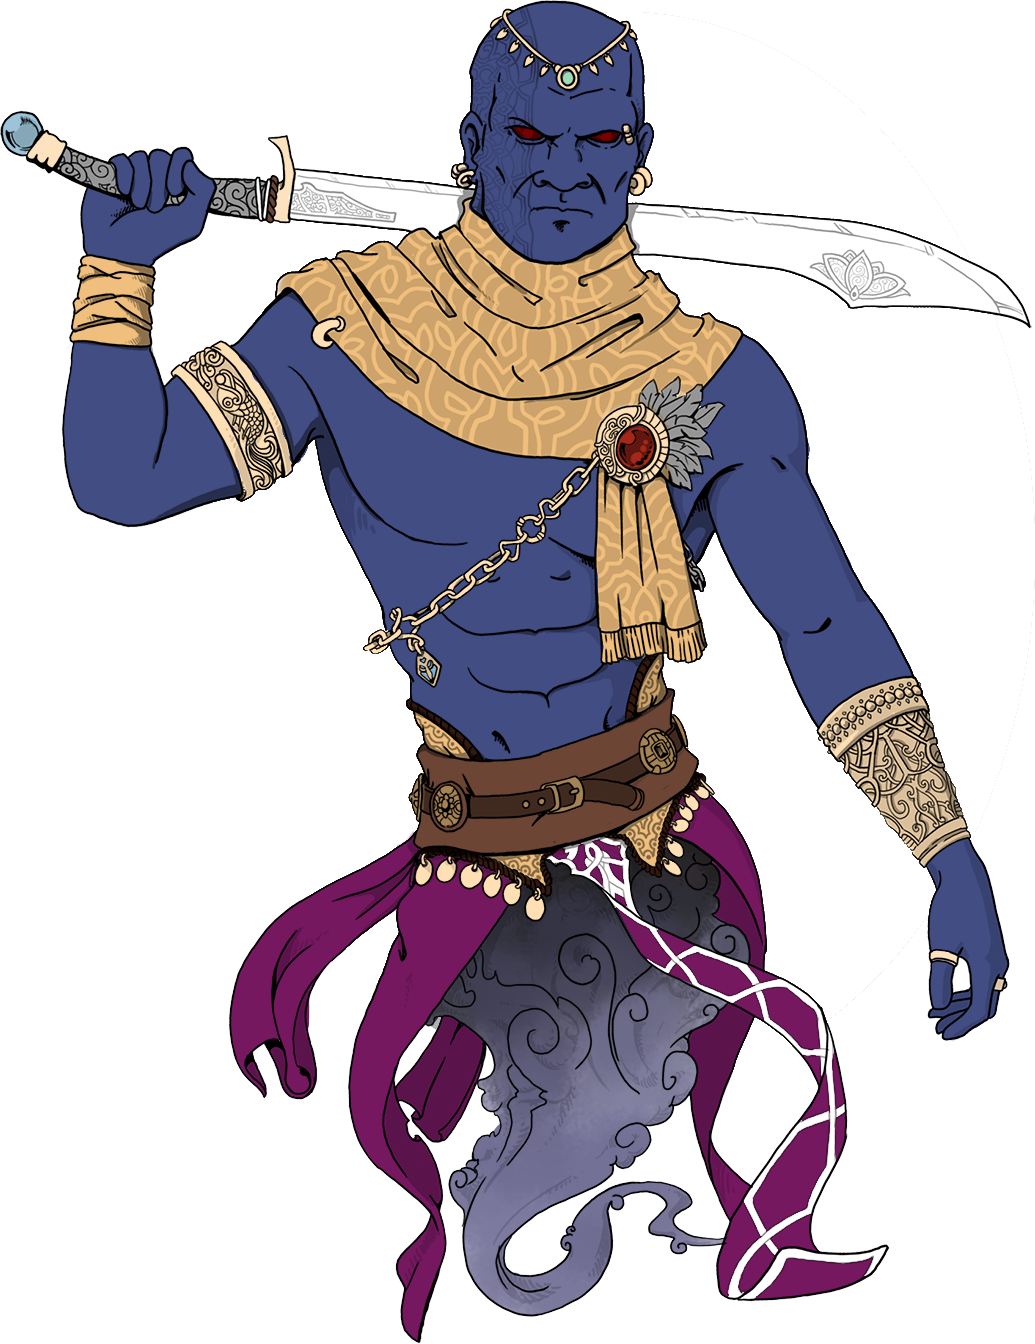
\includegraphics[width=\columnwidth]{Monsters/Genie, Djinni}

\subsection{Djinni, Pasha}\index[monsters]{Pasha}
\statblock{\textbf{Size:} Large

\textbf{Type:} Monster

\textbf{Habitat:} Elemental Plane of Air (Very Rare)

\textbf{Wandering Group:} 1 (Nil)

\textbf{Lair Group:} 1 (Nil)

\textbf{Move:} 40 ft., 120 ft. (Fly)

\textbf{Armor Class:} -2*

\textbf{Hit Dice:} 15** (68 HP)

\textbf{Attacks:} 2x Fist (3d10) 

\textbf{Special:} Immunity to Weapons < +2, Regeneration (3), 

Spell-like Abilities, Whirlwind

\textbf{Save:} W30

\textbf{Alignment:} Chaotic

\textbf{Intelligence:} 14

\textbf{Morale:} 11

\textbf{XP Value:} 4,800}

Pasha are the rulers of the djinn. They appear as blue skinned humans. Despite being magical creatures of chaos, djinn are normally good-natured and friendly.

\textbf{Spell-like Abilities:} A pasha can cast the following spells (as a \nth{15} level caster if appropriate): \iref[spell:Create Food]{Create Food} (3/day), \iref[spell:Woodform]{Woodform} or \iref[spell:Clothform]{Clothform} (3/day), \iref[spell:Stoneform]{Stoneform} or \iref[spell:Ironform]{Ironform} (3/day), \iref[spell:Invisibility]{Invisibility} (3/day), \iref[spell:Phantasmal Force]{Phantasmal Force} (3/day), Grant another’s \iref[spell:Wish]{Wish} (1/day), \iref[spell:Cloudkill]{Cloudkill} (1/day), and \iref[spell:Weather Control]{Weather Control} (1/day).

\textbf{Whirlwind:} A pasha can transform in a single round into a whirlwind 120 feet tall and 10 feet in diameter at the base. While in this form, the pasha can move at a rate of 80 feet, and any creature it engulfs takes 3d12 damage. Creatures of less than 5 hit dice must make a saving throw vs. death ray or be slain.

\subsubsection{Spellcasting}
Pasha can be shamans (to \nth{8} level) or sorcerers (to \nth{12} level).

\subsection{Dolphin}\index[monsters]{Dolphin}
\statblock{\textbf{Size:} Large

\textbf{Type:} Animal

\textbf{Habitat:} Ocean (Common)

\textbf{Wandering Group:} 0 (Nil)

\textbf{Lair Group:} 1d20 (Nil)

\textbf{Move:} 60 ft.

\textbf{Armor Class:} 5

\textbf{Hit Dice:} 3* (14 HP)

\textbf{Attacks:} Ram (2d4)

\textbf{Special:} Detect Magic

\textbf{Save:} D6

\textbf{Alignment:} Lawful

\textbf{Intelligence:} 15

\textbf{Morale:} 10

\textbf{XP Value:} 50}

Dolphins are sapient aquatic mammals related to whales.

Although aquatic, dolphins still breathe air, and need to return to the surface every 15 minutes to breathe.

Dolphins have their own language of clicks and whistles. Dolphins and humanoids can learn to understand each others’ languages, but cannot speak them without magical assistance because of the differences in mouth shape.

Dolphins are generally friendly to humans and demi-humans, although their different culture and environment causes there to be little interaction between the two groups and no trade—something which dolphins have no concept of.

\textbf{Detect Magic:} Dolphins can Detect Magic underwater with a 360-foot range.

\subsubsection{Spellcasting}
Some dolphins can become shamans (of up to \nth{10} level) or sorcerers (of up to \nth{8} level).

\includegraphics[width=\columnwidth]{Monsters/Animals/Dolphin}

\subsection{Donkey}\index[monsters]{Donkey}
\statblock{\textbf{Size:} Medium

\textbf{Type:} Animal

\textbf{Habitat:} Clear, Desert (Common)

\textbf{Wandering Group:} 1d2 (Nil)

\textbf{Lair Group:} 2d12 (Nil)

\textbf{Move:} 40 ft.

\textbf{Armor Class:} 7

\textbf{Hit Dice:} 1+1 (6 HP)

\textbf{Attacks:} Kick (1d3)

\textbf{Special:} None

\textbf{Save:} F1

\textbf{Alignment:} None

\textbf{Intelligence:} 3

\textbf{Morale:} 6

\textbf{XP Value:} 15}

Donkeys are hoofed mammals related to horses. Although smaller and less strong than horses, they are more intelligent.

Unfortunately, this intelligence often makes them less popular as pack animals, since while mostly generally docile they are also very stubborn.

However, if treated gently, donkeys can be more loyal than horses, require less feeding, handle rough terrain better, and make good companions.

\includegraphics[width=\columnwidth]{Monsters/Animals/Donkey}

\subsection{Doppelganger}\index[monsters]{Doppelganger}
\statblock{\textbf{Size:} Medium

\textbf{Type:} Monster

\textbf{Habitat:} Any (Rare)

\textbf{Wandering Group:} 1d6 (Nil)

\textbf{Lair Group:} 1d6 (E)

\textbf{Move:} 30 ft.

\textbf{Armor Class:} 5

\textbf{Hit Dice:} 4* (18 HP)

\textbf{Attacks:} “Weapon” (1d8)

\textbf{Special:} Immunity (Charm, Sleep), Shapechange

\textbf{Save:} F8

\textbf{Alignment:} Chaotic

\textbf{Intelligence:} 9

\textbf{Morale:} 8

\textbf{XP Value:} 125}

Doppelgangers are strange creatures which look like skinny hairless, genderless, featureless humanoids in their natural shape.

\textbf{Shapechange:} A doppelganger is able to “imprint” on a humanoid target, and then take on the exact shape of that target; mimicking equipment and clothing. The doppelganger becomes single-mindedly obsessed with their target and tries to find a way to kill the target and take over their identity.

Doppelgangers seem to have some kind of limited telepathic bond with their target once they have imprinted on them, and gain all the target’s memories. Even spells such as ESP reveal that the doppelganger genuinely believes itself to be the target rather than an impostor.

Should a doppelganger successfully take over a target’s identity, it will remain in that identity for 2d6 days before the imprint wears off and it returns to its normal form and hides until it sees a new target.

\subsubsection{Spellcasting}
Doppelgangers can be shamans (to \nth{6} level) or sorcerers (to \nth{4} level).

\subsection{Dragon}\index[monsters]{Dragon}
\statblock{\textbf{Size:} Varies

\textbf{Type:} Dragon

\textbf{Habitat:} Black: Swamp; Blue: Clear, Desert; 

Gold: Any; Green: Jungle, Woods; Red: Hills, Mountains; 

White: Arctic (Rare); All: Underground in Habitat

\textbf{Wandering Group:} 1 (Nil)

\textbf{Lair Group:} 1d4 (Varies)

\textbf{Move:} 40 ft., 50 ft. (Fly)

\textbf{Armor Class:} Varies

\textbf{Hit Dice:} Varies

\textbf{Attacks:} 2x Claw (Varies) \& Bite (Varies)

\textbf{Special:} Breath Weapon, Wizard Spells (Queen), 

Shapechange (Queen), Swoop

\textbf{Save:} Varies

\textbf{Alignment:} Chaotic

\textbf{Intelligence:} 5 or 15

\textbf{Morale:} 9

\textbf{XP Value:} Varies}

Dragons are great winged lizards that are known for their great power, their treasure hoarding, and for terrorizing large areas of countryside around their lairs.

In fact, this behavior is limited to male dragons which are relatively vicious, bestial and territorial creatures. Female dragons—called dragon queens—are both more powerful and more intelligent than the males, although they are also much rarer.

Dragon queens are still aloof and arrogant in temperament, but they are also social creatures who enjoy entertaining visitors and traveling around exploring human civilizations.

Every twenty years, a female dragon enters a six-month-long breeding frenzy, during which her mind reverts to a bestial nature comparable to that of a male dragon and she flies around visiting all the males she can find. At the end of this period, she will return to her home (and to her normal outlook) and lay a clutch of eggs—each of which will have a different father—and raise the young for the first five to ten years of their lives before they leave her lair to find their own homes.

Dragons of either gender can live for hundreds of years, and continue to grow for most of their life, although even a newly hatched dragon is still a formidable foe.

Dragons come in a variety of colors; black, blue, green, red and white. The scales of a dragon queen are gem-like in appearance. All colors of dragon can interbreed, and the color of children is inherited from the father.

\textbf{Breath Weapon:} A dragon is able to use a breath weapon three times per day, each time doing an amount of damage equal to the dragon’s current hit points. The shape of the breath weapon and the type of damage it does depend on the dragon’s color.

Line shaped breath attacks (from black or blue dragons) affect an area 200 feet long by 5 feet wide.

Cloud shaped breath attacks (from green dragons) affect an area with a 50-foot diameter and 30-foot height in front of the dragon’s mouth. Cone shaped breath attacks (from red and white dragons) affect a conical area 150 feet long and 30 feet wide at the end.

Any creature in the area of the breath attack takes full damage unless it can make a saving throw vs. breath weapon in which case it only takes half damage.

Dragon queens each have an additional breath weapon that they can use instead of their primary one, although they may still only use three breath attacks per day.

\textbf{Crystal:} This breath does normal cold damage, but additionally all unattended non-living items (as well as those worn or carried by creatures who failed their saving throws) in the area of the breath are turned to ice for a period of one hour. This ice will not melt, but may be broken or shattered. Any weapon or armor turned to ice will shatter when struck if a 1-5 is rolled on 1d6. Weapons that shatter do minimum damage and are useless thereafter. Armor that shatters falls off and becomes useless.

\textbf{Darkness:} This breath does normal acid damage, but any victim who fails their saving throw is also surrounded by a Darkness spell with a 15-foot radius that lasts for 1 round per hit die of the dragon (or until dispelled). The dragon can see through this darkness normally.

\textbf{Disease:} This breath does normal poison damage, but any target who fails their saving throw against it is also afflicted with a rotting disease. The target loses 1 hit point per 10 minutes, and is unaffected by healing spells until this disease is cured.

Any non-metal items on a target who failed their saving throw (or any unattended non-metal items breathed on) will rot away in 1d6x10 minutes unless a Cure Disease spell is used on them.

\textbf{Melt:} This breath does normal fire damage but additionally any items carried or worn by creatures that fail their saving throw (or any unattended items breathed on) will begin to melt or burn. Paper is destroyed instantly; cloth and leather is destroyed in one round; other non-metal items in two rounds; metal items in three rounds; and magic items of all types in four rounds (plus one round per point of magical “plus” in the case of weapons and armor). Magical items that bestow fire resistance take twice as long to melt. The melting of items can only be stopped by cooling them—either with water or magically.

\textbf{Vaporize:} This breath does normal lightning damage, but additionally any creatures that fail their saving throw (or any unattended items breathed on) turn to a gaseous form for ten minutes per hit dice of the breathing dragon. Such vaporized items and creatures are invisible and are unable to make any noise or affect any solid object. Living creatures can move at a speed of 20 feet per round if they concentrate.

In any of the above cases, a successful Dispel Magic (with the dragon’s hit dice as the caster level) will remove the effect prematurely.

All dragons are immune to breath weapons of their own type, and automatically make saving throws (if applicable) to any damage of the same basic type as their own breath weapon.

\begin {table}[H]
  \caption{Dragon Breath}
  \begin{tabularx}{\columnwidth}{>{\bfseries}YYYY}
	\thead{Dragon Color} & \thead{Normal Breath} & \thead{Queen Breath} & \thead{Breath Shape}\\
	Black & Acid & Darkness & Line\\
	Blue & Lightning & Vaporize & Line\\
	Green & Poison Gas & Disease & Cloud\\
	Red & Fire & Melt & Cone\\
	White & Cold & Crystal & Cone
  \end {tabularx}
\end {table}

\textbf{Wizard Spells:} Dragons queens know and cast spells as a wizard of the level indicated on \fullref{tab:Dragon Abilities by Age}.

\textbf{Shapechange:} Dragon queens are able to change shape at will into human form. They are able to cast spells in this form but do not retain any of their other abilities.

\textbf{Swoop:} Any dragon that is flying can perform a swoop maneuver in combat which is identical to a Charge maneuver except that the attack does not have to come at the end of the move.

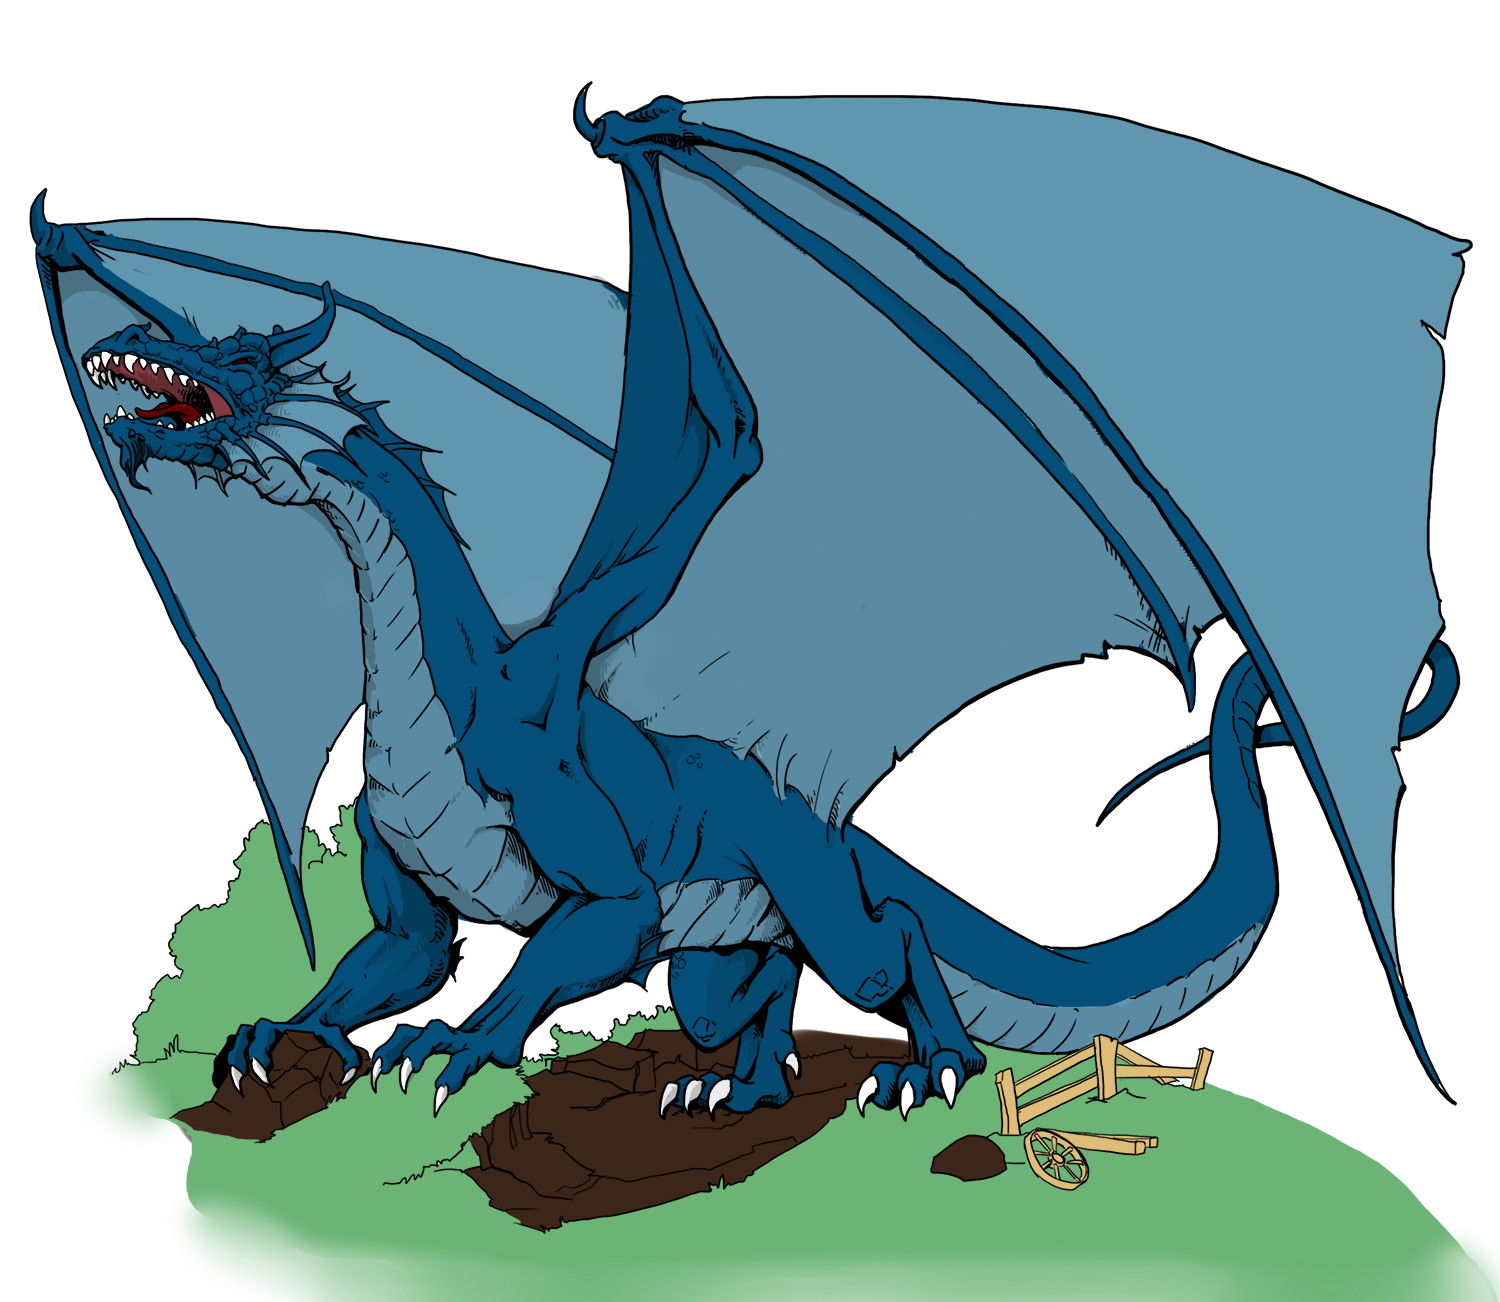
\includegraphics[width=\columnwidth]{Monsters/Dragon}

\end{multicols*}
\begin {table}[H]
  \caption{Dragon Abilities by Age}\label{tab:Dragon Abilities by Age}
	\begin{tabularx}{\columnwidth}{>{\bfseries}ccYccccM{.8in}ccc}
	\thead{} &  \thead{} &  \thead{} &  \thead{} & \thead{Damage} & \thead{} & \thead{} & \thead{}  & \multicolumn{3}{c}{\thead{XP}}\\
	\thead{Age} & \thead{Size} & \thead{Armor Class} & \thead{Hit Dice} & \thead{Claw} & \thead{Bite} & \thead{Save} & \thead{Queen Magic-User Level} & \thead{Treasure} & \thead{Normal} & \thead{Queen}\\
	Very Young (1-5 years) & Small & 3 & 6** (27 HP) & 1d4 & 2d8 & F6 & \nth{2} & H & 950 & 1,075\\
	Young (6-15 years) & Small & 1 & 8** (36 HP) & 1d6 & 3d8 & F8 & \nth{3} & H & 2,300 & 2,850\\
	Sub-Adult (16-25 years) & Medium & -2 & 11** (50 HP) & 2d4 & 6d6 & F11 & \nth{5} & 2xH & 3,500 & 5,100\\
	Young Adult (26-50 years) & Medium & -3 & 14*** (63 HP) & 1d10+1 & 4d8+4 & F28 & \nth{7} & 3xH & 3,500 & 5,500\\
	Adult (51-100 years) & Large & -3 & 16**** (72 HP) & 1d10+2 & 3d8+8 & F36 & \nth{10} & 3xH & 6,250 & 9,550\\
	Old (101-200 years) & Large & -4 & 18**** (81 HP) & 1d10+3 & 3d10+8 & F36 & \nth{12} & 3xH, I & 7,525 & 11,575\\
	Very Old (201-400 years) & Large & -5 & 20**** (90 HP) & 1d12+2 & 4d8+8 & F36 & \nth{15} & 3xH, 2xI & 9,575 & 16,775\\
	Ancient (401+ years) & Large & -6 & 22**** (99 HP) & 4d4 & 6d6+8 & F36 & \nth{18} & 3xH,2xI & 14,000 & 23,000
  \end {tabularx}
\end {table}

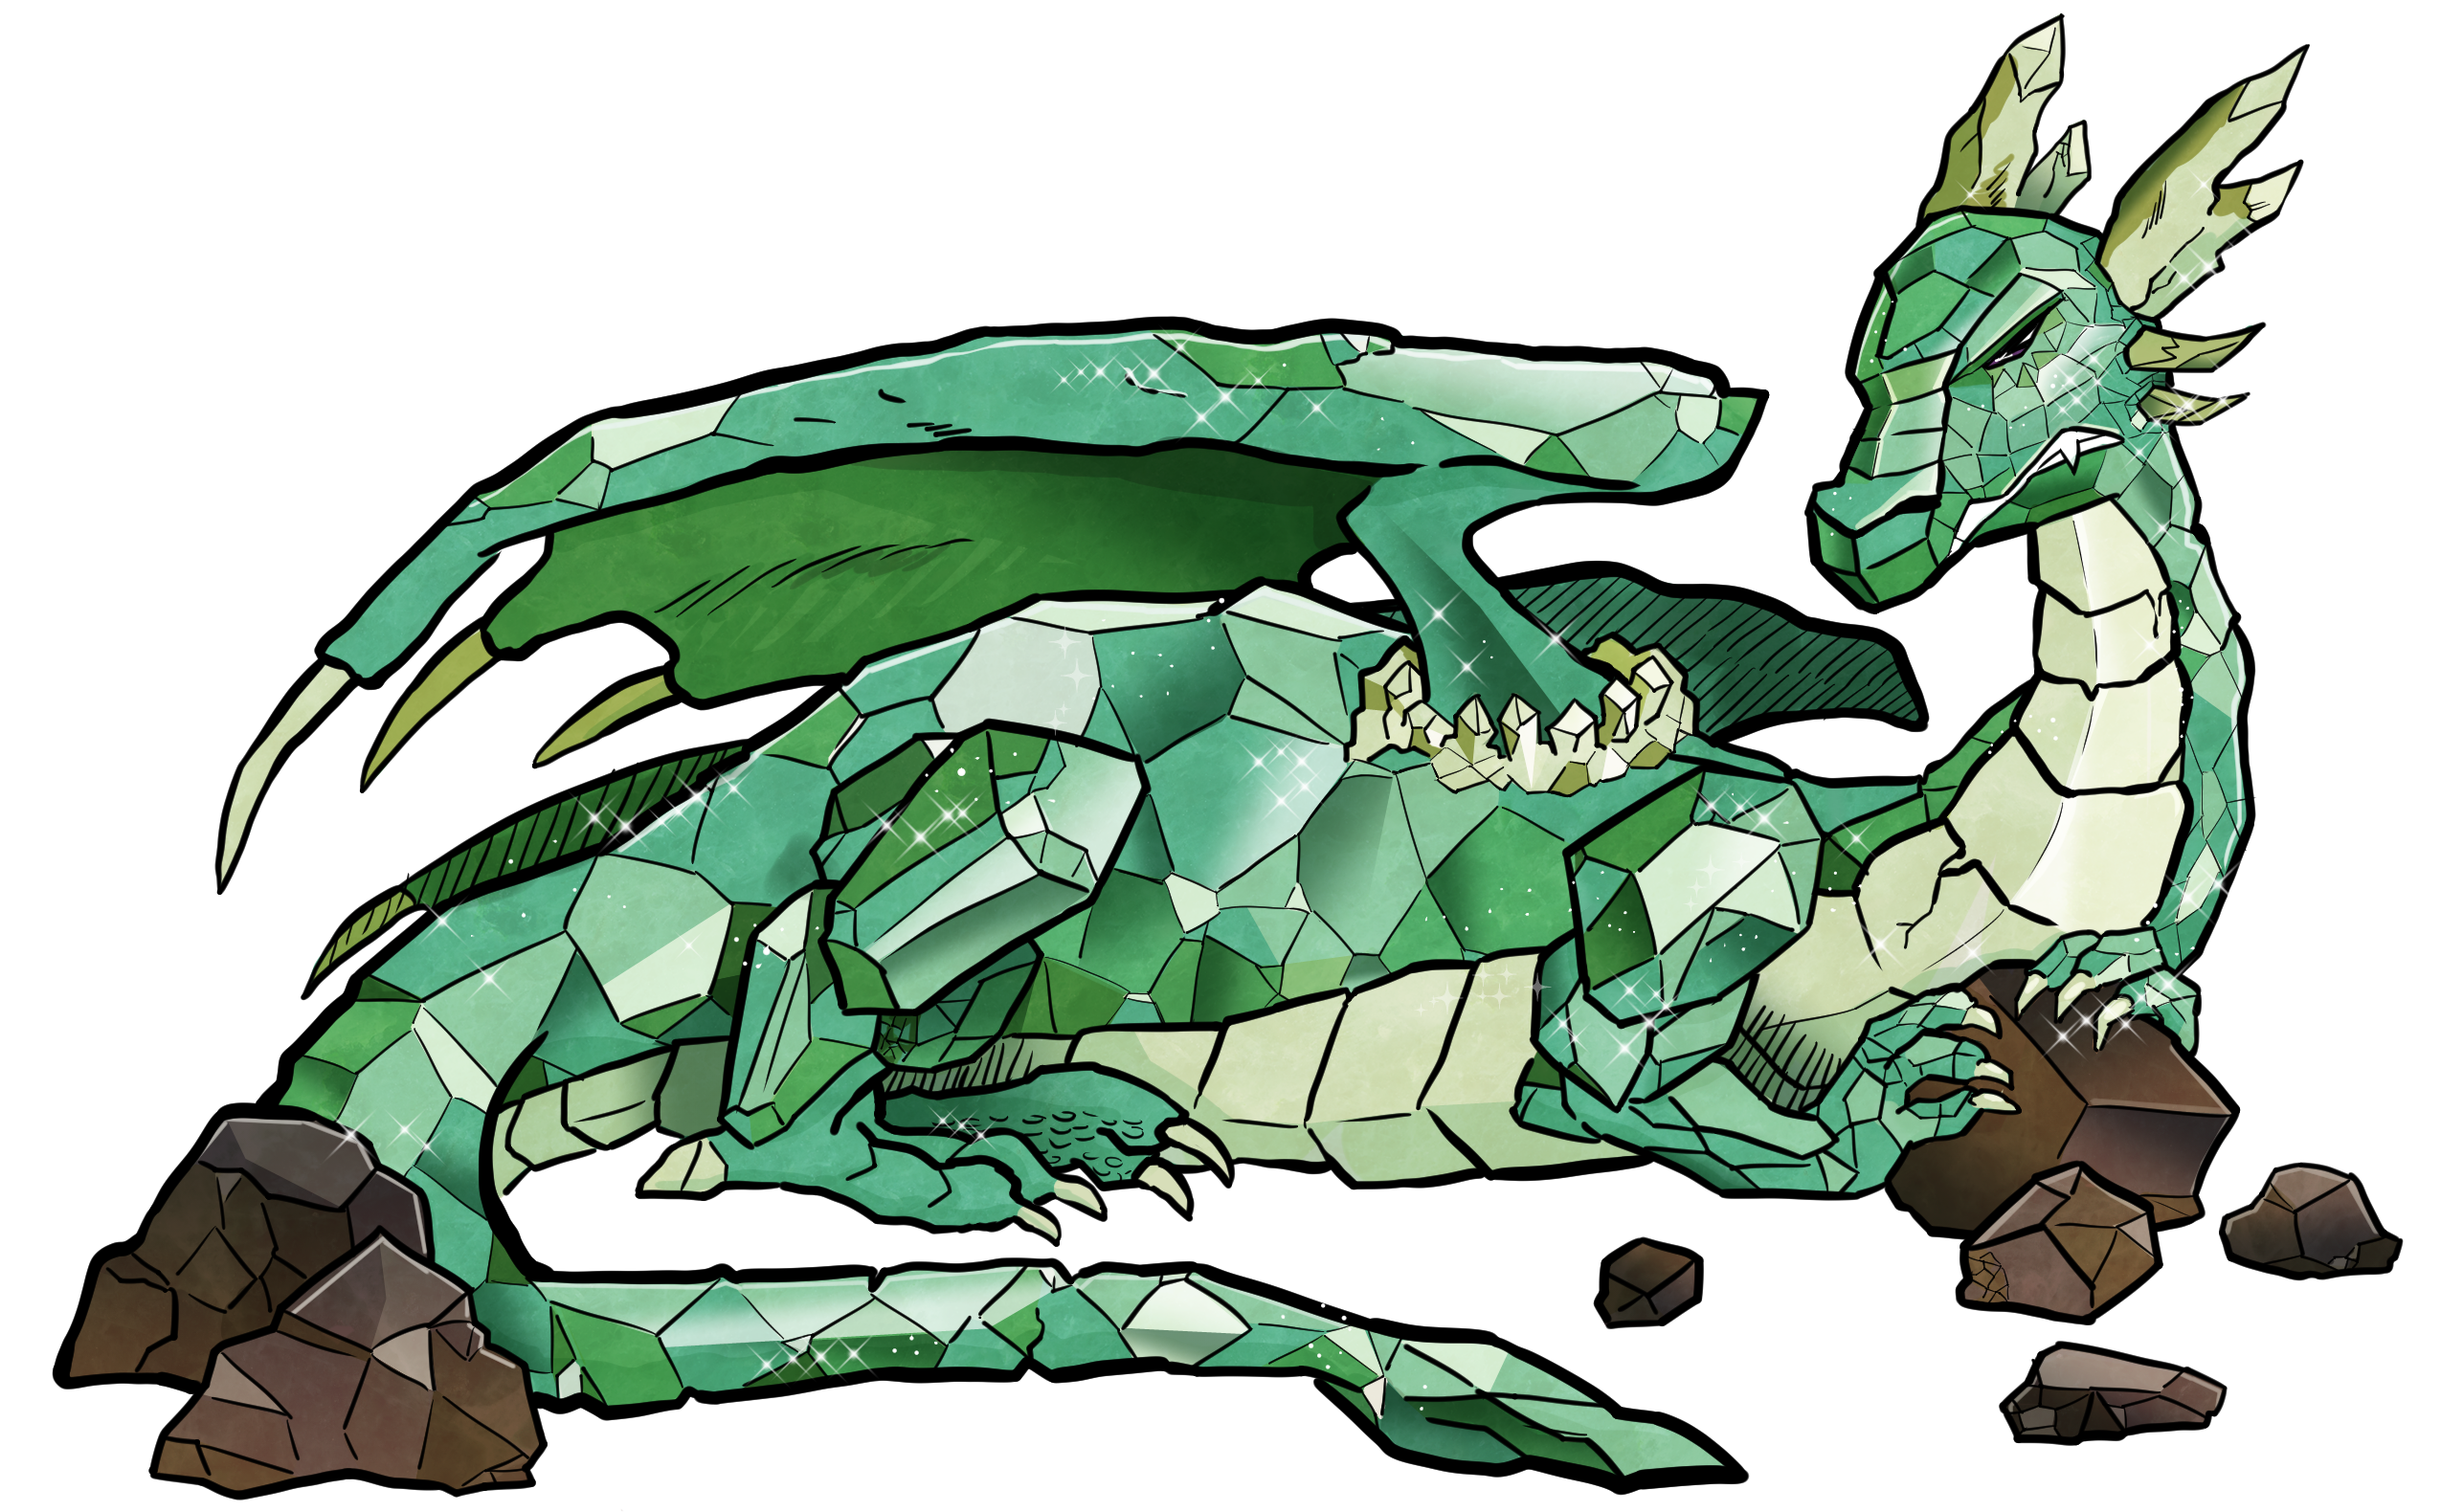
\includegraphics[width=\columnwidth]{Monsters/Dragon, Gem}

\begin{multicols*}{2}

\subsection{Dragon, Skeleton}\index[monsters]{Skeleton Dragon}
\statblock{\textbf{Size:} Large

\textbf{Type:} Undead

\textbf{Habitat:} Any (Very Rare)

\textbf{Wandering Group:} 1 (Nil)

\textbf{Lair Group:} 1 (Nil)

\textbf{Move:} 40 ft., 80 ft. (Fly)

\textbf{Armor Class:} -3*

\textbf{Hit Dice:} 20***** (90 HP)

\textbf{Attacks:} 2x Claw (2d6) \& Bite (1d20+10) or Special

\textbf{Special:} Breath Weapon, Detect Invisibility, 

Immunity (Cold, Fire, Gases, Mind Affecting, 

Poison, Spells < \nth{6} level, Weapons < +3)

\textbf{Save:} F22

\textbf{Alignment:} None

\textbf{Intelligence:} 3

\textbf{Morale:} 12

\textbf{XP Value:} 11,375}

A skeleton dragon is the undead form of a dragon. Despite its skeletal nature, it can still fly and still has a breath weapon.

Because of their powerful nature, skeleton dragons cannot be destroyed using a Dispel Magic spell, and are very resistant to being turned. Skeleton dragons use the Spirit entry on \fullref{tab:Turning Undead by Cleric Level}, and if a cleric gets a ‘D’ result, the skeleton dragon may make a saving throw vs. spells to avoid the effect. If a cleric gets a normal turning result, the turn effect only lasts for 1d4 rounds before the skeleton dragon recovers.

\textbf{Breath Weapon:} Three times per day, a skeleton dragon can breathe a 20-by-20-by-20-foot cloud of poisonous gas. Any within the cloud must make a saving throw vs. poison or die.

\textbf{Detect Invisibility:} Skeleton dragons can see invisible things.

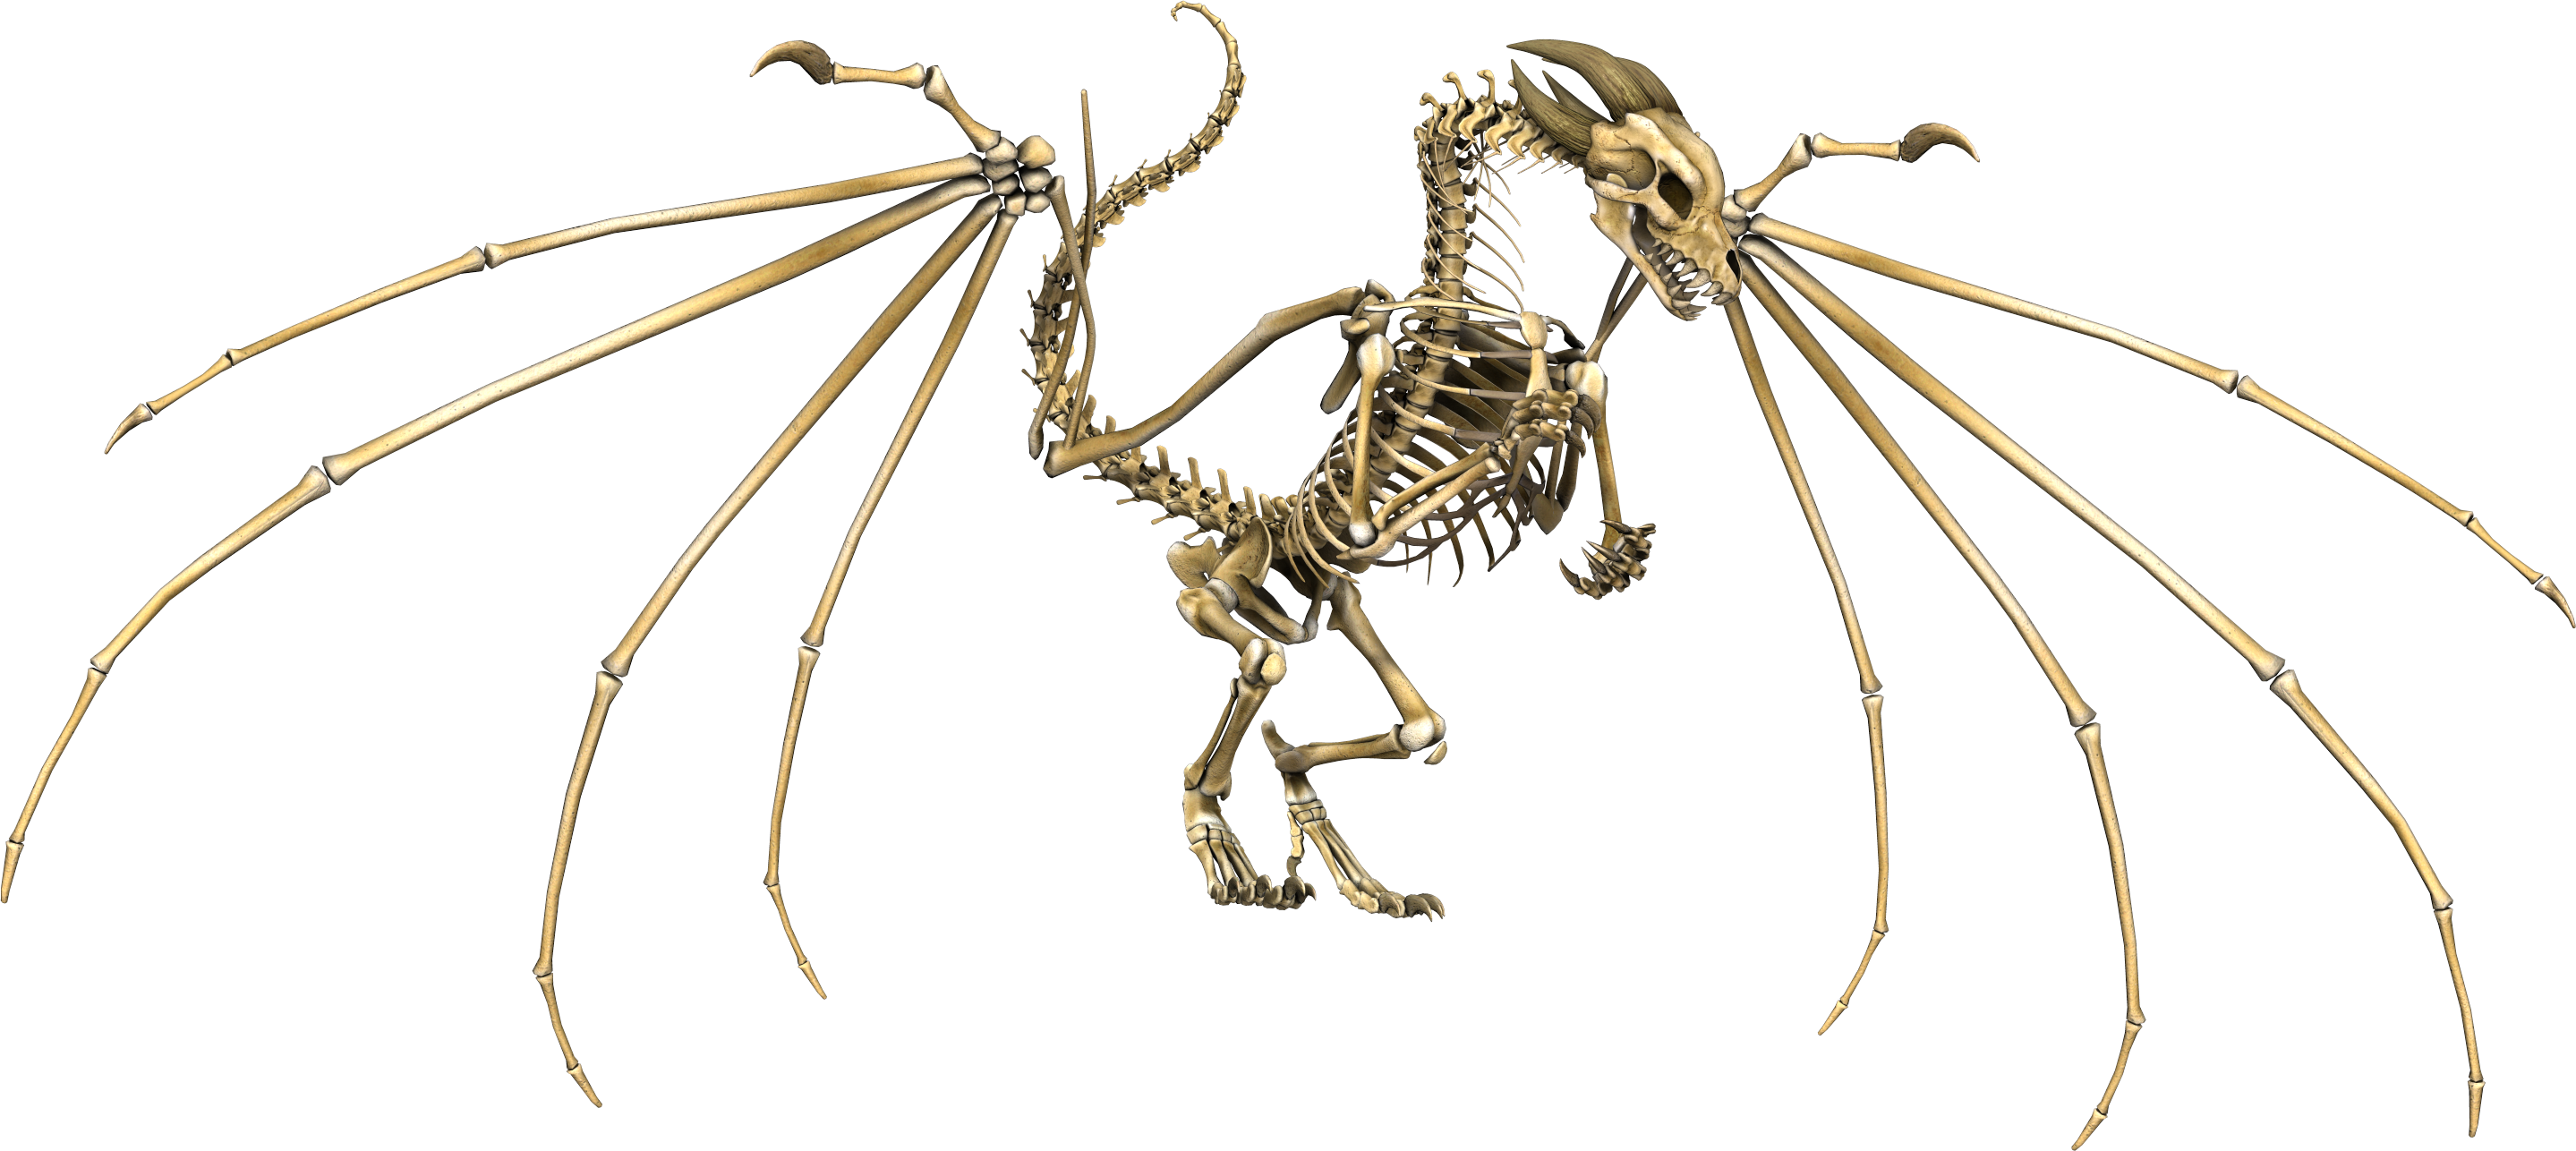
\includegraphics[width=\columnwidth]{Monsters/Dragon, Skeleton}

\subsection{Dragon Turtle}\index[monsters]{Dragon Turtle}
\statblock{\textbf{Size:} Large

\textbf{Type:} Dragon

\textbf{Habitat:} Ocean (Rare)

\textbf{Wandering Group:} 0 (Nil)

\textbf{Lair Group:} 1 (H)

\textbf{Move:} 10 ft., 30 ft. (Swim)

\textbf{Armor Class:} -2

\textbf{Hit Dice:} 30* (135 HP)

\textbf{Attacks:} 2x Claw (1d8) \& Bite (10d6)

\textbf{Special:} Breath Weapon

\textbf{Save:} F15

\textbf{Alignment:} None

\textbf{Intelligence:} 5

\textbf{Morale:} 10

\textbf{XP Value:} 9,000}

Dragon turtles are aquatic relations of true dragons. Although not sapient, they are still rather cunning and have the dragons’ love of treasure.

A dragon turtle is shaped like a sea turtle, but with the head of a dragon.

Dragon turtles normally live in deep water amongst the treasure laden wrecks of ships; occasionally rising up to sink a new ship to add to their collection.

\textbf{Breath Weapon:} Three times per day, a dragon turtle can breathe a cloud of scalding steam in a 50-foot diameter sphere. This cloud of steam does damage equal to the dragon turtle’s current hit point total to all within it, unless they can make a saving throw vs. breath weapon in which case they only take half damage.

\subsection{Drake}
Drakes are lesser cousins of true dragons. They are much smaller than true dragons, being only the size of a human, and stand upright.

Unlike their larger cousins, drakes have no magic use or breath weapon.

Drakes have little interest in human and demi-human society, but they are often found interacting with it as servants of true dragons; especially dragon queens.

\textbf{Immunity to Spells < \nth{5} level:} Drakes are immune to all magic spells of less than \nth{5} level. They can voluntarily drop this immunity by concentrating, for example to receive a cure spell.

\textbf{Rogue Abilities:} In humanoid form, a drake can use all \iref[class:Rogue]{Rogue} abilities as if they were a \nth{5} level \iref[class:Rogue]{Rogue}.

\subsubsection{Elemental Drake}\index[monsters]{Elemental Drake}
\statblock{\textbf{Size:} Large

\textbf{Type:} Dragon

\textbf{Habitat:} Any (Rare)

\textbf{Wandering Group:} 1d4 (2xV)

\textbf{Lair Group:} 1d4 (E)

\textbf{Move:} 40 ft., 10 ft. (Fly)

\textbf{Armor Class:} 0*

\textbf{Hit Dice:} 6**** (27 HP)

\textbf{Attacks:} 2x Claw (1d3) \& Bite (1d8+2)

\textbf{Special:} Immunity (Normal Weapons, 

Spells < \nth{5} level), Shapechange

\textbf{Save:} W12

\textbf{Alignment:} Chaotic

\textbf{Intelligence:} 10

\textbf{Morale:} 9

\textbf{XP Value:} 1,175}

There are four species of elemental drakes, one for each elemental type. Air drakes are blue, earth drakes are brown, fire drakes are red, and water drakes are sea green.

\textbf{Shapechange:} Elemental drakes can change shape at will into an elemental of a particular type, and in that form have the abilities of a 6 hit die elemental of that type.

\subsubsection{Hominal Drake}\index[monsters]{Hominal Drake}
\statblock{\textbf{Size:} Medium

\textbf{Type:} Dragon

\textbf{Habitat:} Any (Rare)

\textbf{Wandering Group:} 1d4 (2xV)

\textbf{Lair Group:} 1d4 (E)

\textbf{Move:} 40 ft., 10 ft. (Fly)

\textbf{Armor Class:} 0*

\textbf{Hit Dice:} 3*** (14 HP)

\textbf{Attacks:} 2x Claw (1d2) \& Bite (1d6)

\textbf{Special:} Immunity to Spells < \nth{5} level, Shapechange

\textbf{Save:} W6

\textbf{Alignment:} Chaotic

\textbf{Intelligence:} 10

\textbf{Morale:} 8

\textbf{XP Value:} 225}

Hominal drakes are tan.

Hominal drakes prefer the company of men and will often take service jobs in human settlements for the opportunities to socialize.

\textbf{Shapechange:} Hominal drakes can change shape at will into a human form, and in that form have the abilities of a \nth{5} level rogue.

\subsubsection{Mountain Drake}\index[monsters]{Mountain Drake}
\statblock{\textbf{Size:} Small

\textbf{Type:} Dragon

\textbf{Habitat:} Hills, Mountains (Rare)

\textbf{Wandering Group:} 1d4 (2xV)

\textbf{Lair Group:} 1d4 (E)

\textbf{Move:} 40 ft., 10 ft. (Fly)

\textbf{Armor Class:} 0*

\textbf{Hit Dice:} 5*** (23 HP)

\textbf{Attacks:} 2x Claw (1d2) \& Bite (2d4)

\textbf{Special:} Immunity to Spells < \nth{5} level, Shapechange

\textbf{Save:} W10

\textbf{Alignment:} Chaotic

\textbf{Intelligence:} 10

\textbf{Morale:} 8

\textbf{XP Value:} 550}

Mountain drakes are white.

Mountain drakes are often found living in dwarf and gnome communities.

\textbf{Shapechange:} Mountain drakes can change shape at will into a dwarf form, and in that form have the abilities of a \nth{5} level dwarf.

\subsubsection{Wood Drake}\index[monsters]{Wood Drake}
\statblock{\textbf{Size:} Medium

\textbf{Type:} Fey

\textbf{Habitat:} Woods (Rare)

\textbf{Wandering Group:} 1d4 (2xV)

\textbf{Lair Group:} 1d4 (E)

\textbf{Move:} 40 ft., 10 ft. (Fly)

\textbf{Armor Class:} 0*

\textbf{Hit Dice:} 4*** (18 HP)

\textbf{Attacks:} 2x Claw (1d2) \& Bite (1d8)

\textbf{Special:} Immunity to Spells < \nth{5} level, 

Invisibility to Mortals, Shapechange

\textbf{Save:} W8

\textbf{Alignment:} Chaotic

\textbf{Intelligence:} 10

\textbf{Morale:} 8

\textbf{XP Value:} 225}

Wood drakes are dark green.

Wood drakes are often found living in elf and halfling communities.

\textbf{Shapechange:} Wood drakes can change shape at will into an elf or halfling form, and in that form have the abilities of a \nth{5} level member of that class.

\subsubsection{As a Class}\index[classes]{Wood Drake}
Wood drakes can be used as a class using the following statistics:

\textbf{Rogue Abilities:} Wood drake PCs start with their rogue abilities while immature and continue to improve them throughout maturity. From \nth{1} to \nth{10} level, wood drakes use their rogue abilities as a rogue with a level equal to the wood drake's hit dice. After \nth{10} level, their rogue abilities are raised one rogue level every other level.

\textbf{Invisibility to Mortals:} Wood drake PCs do not gain this ability till \nth{2} level.

\statblock{\textbf{Ability Requirements:} Dexterity 13

\textbf{Prime Requisite:} Dexterity and Intelligence

\textbf{Ability Modifiers:} None

\textbf{Weapons:} Any one-handed and any missile

\textbf{Natural Attacks:} 2x Claw (1d2) \& Bite (1d3 [-8,00 XP], 1d4 [-6,000 XP], 1d6 [-4,000 XP], 1d8 [Mature])

\textbf{Armor:} Leather armor

\textbf{Natural AC (Drake Form):} 8 (Immature -3), 6 (Immature -2), 4 (Immature -1), 2 (Mature)

\textbf{Special Abilities:} Shapechange, Invisibility to Mortals

\textbf{Magic Item Use:} None, Rogue (Elf or Halfling Form); Elf and Wizard (Chance of Misuse, see \fullref{tab:Wood Drake Magic Item Use})}

\begin {table}[H]
  \caption{Wood Drake Progression}
  \begin{tabularx}{\columnwidth}{>{\bfseries}YYY}
	\thead{Level} & \thead{Experience} & \thead{Hit Dice}\\
	-3 & -16,000 & 1d8\\
	-2 & -12,000 & 2d8\\
	-1 & -8,000 & 3d8\\
	0 & 0 & 4d8\\
	1 & 16,000 & 5d8\\
	2 & 48,000 & -\\
	3 & 112,000 & 6d8\\
	4 & 240,000 & 7d8\\
	5 & 500,000 & -\\
	6 & 800,000 & 8d8\\
	7 & 1,100,000 & 9d8\\
	8 & 1,400,000 & -\\
	9 & 1,700,000 & 10d8\\
	10 & 2,000,000 & 10d8+1\\
	11+ & +250,000 & +1 HP
  \end {tabularx}
\end {table}

\begin {table}[H]
  \caption{Wood Drake Magic Item Use}\label{tab:Wood Drake Magic Item Use}
  \begin{tabularx}{\columnwidth}{>{\bfseries}YYYYY}
	\thead{} & \multicolumn{4}{c}{\thead{d\% Result}}\\
	\thead{Level} & \thead{Success} & \thead{Failure} & \thead{Backfire} & \thead{Unexpected}\\
	1 & 01-05 & 6-89 & 90-99 & 00\\
	2 & 01-05 & 6-89 & 90-98 & 99-00\\
	3 & 01-10 & 11-89 & 90-97 & 98-00\\
	4 & 01-15 & 16-89 & 90-96 & 97-00\\
	5 & 01-15 & 16-89 & 90-95 & 96-00\\
	6 & 01-20 & 21-89 & 90-94 & 95-00\\
	7 & 01-20 & 21-89 & 90-93 & 94-00\\
	8 & 01-25 & 26-89 & 90-92 & 93-00\\
	9 & 01-25 & 26-89 & 90-91 & 92-00\\
	10+ & 01-30 & 31-89 & 90 & 91-00
  \end {tabularx}
\end {table}

\subsection{Dryad}\index[monsters]{Dryad}
\monsterimage{Monsters/Dryad}{\statblock{\textbf{Size:} Medium

\textbf{Type:} Humanoid

\textbf{Habitat:} Woods (Rare)

\textbf{Wandering Group:} 0 (Nil)

\textbf{Lair Group:} 1d6 (D)

\textbf{Move:} 40 ft.

\textbf{Armor Class:} 5

\textbf{Hit Dice:} 2* (9 HP)

\textbf{Attacks:} Weapon (By weapon)

\textbf{Special:} Charm Person, Tree Bind

\textbf{Save:} E4

\textbf{Alignment:} Neutral

\textbf{Intelligence:} 14

\textbf{Morale:} 6

\textbf{XP Value:} 25}}

Dryads are forest spirits who live inside trees. Although dryads are technically asexual, they always appear as beautiful females when they leave their trees.

Dryads are usually peaceful and non-violent unless severely provoked.

\textbf{Charm Person:} Dryads are able to cast a Charm Person spell at will (with a -2 penalty to saving throws). They will normally charm attackers and persuade them to go off and do some deed that will help the dryad’s forest. Occasionally, a dryad will take a liking to a mortal and charm them into living in the tree with them and becoming their servant.

\textbf{Tree Bind:} A dryad is inherently bound to her tree, and can only survive for ten minutes if taken more than 240 feet away from it. Similarly, killing the tree will kill the dryad.

A dryad can merge with or leave her tree at will, and can take others with her. Inside a dryad tree is a softly lit extra-dimensional space the size of a cottage (usually with furniture made of wood and soft leaves). People inside the tree can see out through windows, but there is no door and the windows are not apparent from the outside.

\subsubsection{Spellcasting}
Dryads can be shamans (to \nth{10} level) or sorcerers (to \nth{4} level).

\subsubsection{As a Class}\index[classes]{Dryad}
Dryads can be used as a class using the following statistics:

\statblock{\textbf{Ability Requirements:} Wisdom 8, Charisma 12

\textbf{Prime Requisite:} Wisdom and Charisma

\textbf{Ability Modifiers:} None

\textbf{Weapons:} Blowgun, dagger, pistol, net, sling, staff, whip

\textbf{Armor:} None

\textbf{Natural AC:} 7

\textbf{Special Abilities:} Charm Person, Tree Bind

\textbf{Magic Item Use:} Cleric (Non-Weapons)}

\begin {table}[H]
  \caption{Dryad Progression}
  \begin{tabularx}{\columnwidth}{>{\bfseries}YYYYY}
	\thead{Level} & \thead{Experience} & \thead{Hit Dice}\\
	-1 & -3,000 & 1d8\\
	0 & 0 & 2d8\\
	1 & 3,000 & -\\
	2 & 9,000 & 3d8\\
	3 & 21,000 & -\\
	4 & 45,000 & 4d8\\
	5 & 95,000 & -\\
	6 & 190,000 & 5d8\\
	7 & 380,000 & -\\
	8 & 680,000 & 6d8\\
	9 & 980,000 & -\\
	10 & 1,280,000 & 7d8\\
	11+ & +300,000 & +1 HP
  \end {tabularx}
\end {table}

\subsection{Dwarf}\index[monsters]{Dwarf}
\statblock{\textbf{Size:} Medium

\textbf{Type:} Demi-human

\textbf{Habitat:} Hills, Mountains (Common)

\textbf{Wandering Group:} 1d6 (Q+S)

\textbf{Lair Group:} 5d8 (G)

\textbf{Move:} 20 ft.

\textbf{Armor Class:} 4

\textbf{Hit Dice:} 1 (5 HP)

\textbf{Attacks:} Weapon (By weapon)

\textbf{Save:} D1

\textbf{Special:} As \nth{1} level Dwarf

\textbf{Alignment:} Lawful

\textbf{Intelligence:} 10

\textbf{Morale:} 10

\textbf{XP Value:} 10}

Dwarves are slightly shorter than humans but are similar in weight due to their stockier build. Skin and hair color shows the same range as humans, although both male and female dwarves tend to have slightly more facial and body hair than humans and both sexes usually sport beards.

Traditionally, dwarves live in mountainous areas near humans, where they live underground and use their mining and metal-working skills to make goods and tools that they can trade with the humans for food and textiles.

Dwarves are an inherently non-magical race, and possess no magic users or clerics of their own—not even being able to produce the lesser shamans that goblins and giants—their traditional enemies—are able to field in battle. However, this lack of magical ability makes dwarves much more resilient and able to resist magical attacks.

\subsection{Efreeti}\index[monsters]{Efreeti}
\begin {table}[H]
	\normalfont
	\begin{tabularx}{\columnwidth}{@{}>{\bfseries}XXX@{}}
	\hiderowcolors
	& \textbf{Prime Plane} & \textbf{Home Plane}\\
	Size: & Large & Large\\
	Type: & Extraplanar, Monster & Monster\\
	Habitat: & Desert (Rare) & Elemental Plane of Fire (Rare)\\
	Wandering Group: & 1 (Nil) & 1d4 (Nil)\\
	Lair Group: & 1 (Nil) & 1d100 (Nil)\\
	Move: & 30 ft., 80 ft. (Fly) & 80 ft. (Fly)\\
	Armor Class: & 3 & 1\\
	Hit Dice: & 10* (45 HP) & 10* (45 HP)\\
	Attacks: & Fist (2d8) & Fist (2d8)\\
	Save: & F15 & F15\\
	Special: & Pillar of Flame, Spell-like Abilities & Immunity (\nth{1} level Spells, Earth, Normal Weapons), Pillar of Flame, Spell-like Abilities\\
	Alignment: & Chaotic & Chaotic\\
	Intelligence: & 14 & 14\\
	Morale: & 12 & 8\\
	XP Value: & 1,750 & 1,750\\
	\showrowcolors
  \end {tabularx}
\end {table}

Efreet are desert dwelling spirits. They appear as muscular and horned red skinned humans. As magical creatures of chaos, efreet are cruel and domineering.

\textbf{Pillar of Flame:} An efreeti can transform over the course of five rounds into a pillar of flame 12 feet tall and 5 feet in diameter at the base. While in this form, the efreeti ignites all flammable objects within 5 feet and does an additional 1d8 fire damage with its fist attacks.

\textbf{Spell-like Abilities:} An efreeti can cast the following spells 3 times per day (as a \nth{10} level caster if appropriate): \iref[spell:Create Food]{Create Food}, \iref[spell:Woodform]{Woodform} or \iref[spell:Clothform]{Clothform}, \iref[spell:Stoneform]{Stoneform} or \iref[spell:Ironform]{Ironform}, \iref[spell:Invisibility]{Invisibility}, and \iref[spell:Wall of Fire]{Wall of Fire}.

\subsubsection{Home Plane}
Efreeti originate from the Elemental Plane of Fire.

\textbf{Detect Invisibility:} Efreeti can see invisible creatures within 120 feet.

\subsubsection{Spellcasting}
Efreeti can be shamans (to \nth{6} level) or sorcerers (to \nth{4} level).

\subsubsection{Efreeti, Amir}\index[monsters]{Amir}
\statblock{\textbf{Size:} Large

\textbf{Type:} Monster

\textbf{Habitat:} Elemental Plane of Fire (Very Rare)

\textbf{Wandering Group:} 1 (Nil)

\textbf{Lair Group:} 1 (Nil)

\textbf{Move:} 40 ft., 120 ft. (Fly)

\textbf{Armor Class:} -2*

\textbf{Hit Dice:} 20*** (90 HP)

\textbf{Attacks:} 2x Fist (3d10)

\textbf{Save:} W36

\textbf{Special:} Immunity to Weapons < +2, Pillar of Flame, 

Regeneration (2), Spell-like Abilities

\textbf{Alignment:} Chaotic

\textbf{Intelligence:} 14

\textbf{Morale:} 11

\textbf{XP Value:} 7,775}

Amir are the rulers of the efreet. They appear as horned muscular red skinned humans. As magical creatures of chaos, efreet are cruel and domineering.

\textbf{Pillar of Flame:} An amir can transform in a single round into a pillar of flame 30 feet tall and 5 feet in diameter at the base. While in this form, the amir ignites all flammable objects within 15 feet and does an additional 2d8 fire damage with its fist attacks.

\textbf{Spell-like Abilities:} An amir can cast the following spells (as a \nth{20} level caster if appropriate): \iref[spell:Create Food]{Create Food} (3/day), \iref[spell:Woodform]{Woodform} or \iref[spell:Clothform]{Clothform} (3/day), \iref[spell:Stoneform]{Stoneform} or \iref[spell:Ironform]{Ironform} (3/day), \iref[spell:Invisibility]{Invisibility} (3/day), \iref[spell:Wall of Fire]{Wall of Fire} (3/day), Grant another’s \iref[spell:Wish]{Wish} (1/day), \iref[spell:Explosive Cloud]{Explosive Cloud} (1/day), and \iref[spell:Fireball]{Fireball} (1/day).

\subsubsection{Spellcasting}
Amir can be shamans (to \nth{12} level) or sorcerers (to \nth{8} level).

\subsection{Eldritch Abomination}\index[monsters]{Eldritch Abomination}
\statblock{\textbf{Size:} Large

\textbf{Type:} Exalted, Extraplanar

\textbf{Habitat:} Aether, Void (Very Rare)

\textbf{Wandering Group:} 1 (Nil)

\textbf{Lair Group:} 0 (Nil)

\textbf{Move:} 6 miles (or Voidspeed)

\textbf{Armor Class:} -20*

\textbf{Hit Dice:} 150******* (675 HP)

\textbf{Attacks:} 40 x Tentacle (1d100+Special)

\textbf{Power Reserve:} 4,500

\textbf{Save:} I23

\textbf{Special:} Anti-Magic, Immortal Abilities, 

Immunity to Mortal Magic, Powers

\textbf{Alignment:} Chaotic

\textbf{Intelligence:} 100

\textbf{Morale:} 11

\textbf{XP Value:} 202,500}

An eldritch abomination is a shifting horror of absolutely staggering size. Although the above statistics list the attack type of eldritch abominations as being via tentacles, eldritch abominations are remarkably varied in appearance and make-up, and may actually be striking with body parts other than tentacles. For example, some are clouds of smoky gas-like material; others appear crystalline or metallic; still others appear to be simply patches of color of an indescribable hue. In truth, eldritch abominations are simply not made of the same sort of matter that we are, and our senses are only able to approximate their true forms.

Eldritch abominations are incredibly rare, and are almost never found within a Celestial Sphere. In fact the merest detection of an eldritch abomination near an inhabited sphere is enough to mobilize all the \iref[chap:Immortals]{Immortals} into action to try to defeat it or drive it away.

Eldritch abominations come from some other part of the universe, where they seem to fulfill the same role that \iref[chap:Immortals]{Immortals} do in the local environment.

Eldritch abominations seem to be somehow offended or repulsed by Celestial Spheres and the matter that comes from them, and will often try to destroy such things. However, they will usually completely ignore mortal level creatures that they encounter, as such small fry are completely below their notice (to the extent of simply ploughing through a ship and destroying it rather than moving out of the way).

However, some mad souls have very occasionally been known to make contact with an eldritch abomination and get themselves made into clerics in exchange for promises to aid the abomination in destroying the cleric’s world.

\iref[chap:Immortals]{Immortals} fight an intermittent war with the eldritch abominations; driving them away from populated Celestial Spheres. Some \iref[chap:Immortals]{Immortals} have tried to communicate with eldritch abominations rather than fight them, but report that communication is almost impossible as there is little in terms of a common frame of reference to use as a basis for communication.

It is not known what the home of eldritch abominations is like. \iref[chap:Immortals]{Immortals} guess that they have something similar to Celestial Spheres (but which splits the Luminiferous Aether up in a completely different way to the ether/air/fire/earth/water split that we are used to) and that they maybe even have something similar to Outer Planes—but no-one has ever returned with reports of seeing such things.

Eldritch abominations are only hit by +5 weapons or better.

\textbf{Anti-Magic:} Eldritch abominations have a 99\% Anti-Magic against \iref[sec:Immortal Level Spells]{Immortal Level Spells}.

\textbf{Immortal Abilities:} Eldritch abominations have all the abilities (to take on Spirit Form or Mortal Form and so on) that \iref[chap:Immortals]{Immortals} have.

\textbf{Powers:} Eldritch abominations can spend their power points on all \iref[sec:Immortal Level Spells]{Immortal Level Spells}.

\textbf{Tentacle:} Although an abomination is capable of making 40 attacks per round, it is unable to bring more than 20 attacks to bear against a single opponent at once.

\subsection{Elemental}\label{sec:Elemental}
\monsterimage{Monsters/Elemental, Earth}{\statblock{\textbf{Size:} Varies

\textbf{Type:} Extraplanar

\textbf{Habitat:} Air: Clear, Desert, Mountains, 

Ocean; Earth: Hills, Mountains, 

Underground; Fire: Desert; 

Water: River, Ocean (Common)

\textbf{Wandering Group:} 1 (Nil)

\textbf{Lair Group:} 1 (Nil)

\textbf{Move:} Varies

\textbf{Armor Class:} Varies

\textbf{Hit Dice:} Varies

\textbf{Attacks:} Bash (Varies)

\textbf{Save:} Varies

\textbf{Special:} Resistance to Damage, Varies

\textbf{Alignment:} Neutral

\textbf{Intelligence:} 9

\textbf{Morale:} 10

\textbf{XP Value:} Varies}}

Elementals are sapient creatures made of elemental matter from one of the Elemental Planes.

Elementals of all sizes exist on the Elemental Planes, but they all have common statistics.

\textbf{Resistance to Damage:} When an elemental is hit by damage from a source that it takes double damage from, it can make a saving throw vs. spells to only take normal damage instead. Although elementals of each type are shown on \fullref{tab:Elementals by Element} as taking normal damage from their own element, this applies only to magical damage or attacks from other elementals, and does not apply to mundane environmental damage.

An elemental does not take any environmental damage from its own element.

\subsubsection{Air Elemental}\index[monsters]{Air Elemental}\label{sec:Air Elemental}
An air elemental appears as a whirlwind that is 2 feet tall per hit die and 1 foot in diameter per two hit dice.

\textbf{Air Mastery:} An air elemental does an extra 1d8 damage to any flying creature that it hits.

\textbf{Whirlwind:} Any creature of 2 hit dice or less that an air elemental hits in combat must make a saving throw vs. death ray or be swept away.

\subsubsection{Earth Elemental}\index[monsters]{Earth Elemental}
An earth elemental appears as a humanoid figure made of soil and gravel that is 1 foot tall per hit die. Earth elementals cannot cross water that is wider than their height.

\textbf{Earth Mastery:} An earth elemental does an extra 1d8 damage to any creature it hits that is on the ground.

\subsubsection{Fire Elemental}\index[monsters]{Fire Elemental}
A fire elemental appears as a roughly conical bonfire 1 foot tall per hit die and 1 foot in diameter at the base per hit die. Fire elementals cannot cross water that is wider than their height.

\textbf{Fire Mastery:} A fire elemental does an extra 1d8 damage to any cold-based creature.

\subsubsection{Water Elemental}\index[monsters]{Water Elemental}
A water elemental appears as a wave of water 1 foot tall per two hit dice and 1 foot wide per hit dice. Water elementals cannot move more than 60 feet from a body of water.

\textbf{Water Mastery:} A water elemental does an extra 1d8 damage to any creature it hits that is in water.

\subsubsection{Elemental Ruler}\index[monsters]{Elemental Ruler}
Elementals are ruled by massive Exalted emperors. They are twice the size that their hit dice would otherwise indicate.

\textbf{Crushing Blow:} Any creature hit by an elemental ruler must make a saving throw vs. death ray or be crushed and killed by the blow.

\textbf{Immunities:} Elemental rules are immune to charm, hold, illusions, instant death, poison, spells > \nth{6} level, and weapons < +4.

\begin {table}[H]
  \caption{Elementals by Size}
  \begin{tabularx}{\columnwidth}{>{\bfseries}cYYYY}
	\thead{Hit Dice} & \thead{Armor Class} & \thead{Damage} & \thead{Save} & \thead{XP Value}\\
	2 (9 HP) & 5 & 1d2 & F2 & 20\\
	4 (18 HP) & 4 & 1d4 & F4 & 75\\
	6 (27 HP) & 3 & 1d6 & F6 & 275\\
	8 (36 HP) & 2 & 1d8 & F8 & 650*\\
	10 (45 HP) & 1 & 2d6 & F10 & 1,000\\
	12 (54 HP) & 0 & 2d8 & F12 & 1,250**\\
	14 (63 HP) & -1 & 2d10 & F14 & 1,500\\
	16 (72 HP) & -2 & 3d8 & F16 & 1,850***\\
	18 (81 HP) & -3 & 3d10 & F18 & 2,125\\
	20 (90 HP) & -4 & 4d8 & F20 & 2,375\\
	22 (99 HP) & -5 & 5d8 & F22 & 2,750\\
	24 (108 HP) & -6 & 6d8 & F24 & 3,250\\
	26 (117 HP) & -7 & 7d8 & F26 & 3,750\\
	28 (126 HP) & -8 & 8d8 & F28 & 4,250\\
	30 (135 HP) & -9 & 9d8 & F30 & 4,750\\
	32 (144 HP) & -10 & 10d8 & F32 & 5,250\\
	40*** (180 HP) & -11* & 8d12 & F36 & 27,500\\
	50*** (225 HP) & -12* & 9d12 & F36 & 37,500\\
	60*** (270 HP) & -13* & 10d12 & F36 & 47,500\\
	70*** (315 HP) & -14* & 11d12 & F36 & 57,500\\
	80*** (360 HP) & -15* & 12d12 & F36 & 67,500\
  \end {tabularx}
	* Size of elemental conjured by staff\\
	** Size of elemental conjured by device\\
	*** Size of elemental conjured by spell
\end {table}

\begin {table}[H]
  \caption{Elementals by Element}\label{tab:Elementals by Element}
  \begin{tabularx}{\columnwidth}{>{\bfseries}YYYYY}
	\thead{} & \thead{} & \multicolumn{3}{c}{\thead{Damage}}\\
	\thead{Element} & \thead{Move} & \thead{Double} & \thead{Normal} & \thead{Minimum}\\
	Air & 120 ft. (Fly) & Earth & Air, Fire & Water\\
	Earth & 20 ft. & Fire & Earth, Water & Air\\
	Fire & 40 ft. & Water & Fire, Air & Earth\\
	Water & 20 ft., 60 ft, (Swim) & Air & Water, Earth & Fire
  \end {tabularx}
\end {table}

\subsection{Elephant}\index[monsters]{Elephant}\label{monster:Elephant}
\statblock{\textbf{Size:} Large

\textbf{Type:} Animal

\textbf{Habitat:} Clear, Woods (Rare)

\textbf{Wandering Group:} 1 (Nil)

\textbf{Lair Group:} 3d8 (Nil)

\textbf{Move:} 40 ft.

\textbf{Armor Class:} 5

\textbf{Hit Dice:} 9* (41 HP)

\textbf{Attacks:} 2x Tusk (2d4) or Trample (4d8)

\textbf{Save:} F5

\textbf{Special:} Trample

\textbf{Alignment:} None

\textbf{Intelligence:} 2

\textbf{Morale:} 8

\textbf{XP Value:} 1,600}

Elephants are large mammals with prehensile trunks.

While normally peaceful, elephants do not hesitate to defend themselves or their young from potential attack.

Although elephants have no listed treasure, the tusks of an adult (of either sex) can be sold for approximately 1,000 gp.

\textbf{Trample:} Elephants can trample over anything smaller than itself that gets in its way. Any such victim suffers 4d8 points of damage. The trample is treated as if doing the Charge action.

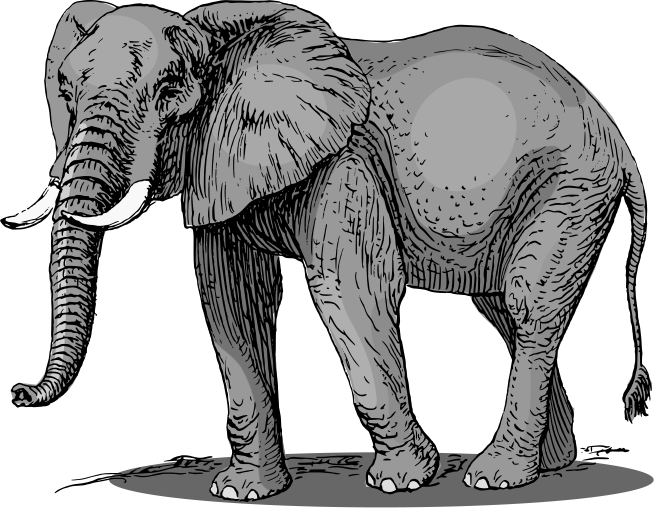
\includegraphics[width=\columnwidth]{Monsters/Animals/Elephant}

\subsection{Elephant, Prehistoric}\index[monsters]{Prehistoric Elephant}
\statblock{\textbf{Size:} Large

\textbf{Type:} Animal

\textbf{Habitat:} Clear, Woods (Very Rare)

\textbf{Wandering Group:} 1 (Nil)

\textbf{Lair Group:} 2d8 (Nil)

\textbf{Move:} 40 ft.

\textbf{Armor Class:} 3

\textbf{Hit Dice:} 15 (68 HP)

\textbf{Attacks:} 2x Tusk (2d6) or Trample (4d8)

\textbf{Save:} F8

\textbf{Special:} Trample

\textbf{Alignment:} None

\textbf{Intelligence:} 2

\textbf{Morale:} 8

\textbf{XP Value:} 1,650}

Prehistoric elephants are elephants with long woolly hair.

While normally peaceful, prehistoric elephants do not hesitate to defend themselves or their young from potential attack.

Although prehistoric elephants have no listed treasure, the tusks of an adult (of either sex) can be sold for approximately 1,500 gp.

\textbf{Trample:} Prehistoric elephants can trample over anything smaller than itself that gets in its way. Any such victim suffers 4d8 points of damage. The trample is treated as if doing the Charge action.

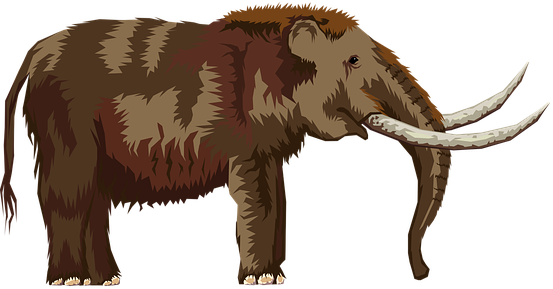
\includegraphics[width=\columnwidth]{Monsters/Animals/Elephant, Prehistoric}

\subsection{Elf}\index[monsters]{Elf}
\statblock{\textbf{Size:} Medium

\textbf{Type:} Demi-human

\textbf{Habitat:} Woods (Rare)

\textbf{Wandering Group:} 1d4 (S+T)

\textbf{Lair Group:} 4d12 (E)

\textbf{Move:} 40 ft.

\textbf{Armor Class:} 5

\textbf{Hit Dice:} 1* (5 HP)

\textbf{Attacks:} Weapon (By weapon)

\textbf{Save:} E1

\textbf{Special:} As \nth{1} level Elf

\textbf{Alignment:} Chaotic

\textbf{Intelligence:} 13

\textbf{Morale:} 8

\textbf{XP Value:} 6}

Elves are slender and graceful humanoids. They show a similar range of skin colors to those of humans in terms of shade, but the hue of their skin tends to be more yellow-brown than that of humans giving them a coloration resembling that of wood anywhere from light pine through to dark ebony. The ears of elves are pointed.

Elves have no body or facial hair, although the hair on their heads is luxuriant, and changes color throughout their life like the colors of leaves change through seasons—starting a light green and slowly darkening, as the elf matures before changing to brown, gold and red in old age.

\subsection{Elf, Aquatic}\index[monsters]{Aquatic Elf}
\statblock{\textbf{Size:} Medium

\textbf{Type:} Demi-human

\textbf{Habitat:} Ocean (Common)

\textbf{Wandering Group:} 1d6 (S+T)

\textbf{Lair Group:} 4d6 (E)

\textbf{Move:} 40 ft., 80 ft. (Swim)

\textbf{Armor Class:} 5

\textbf{Hit Dice:} 1* (5 HP)

\textbf{Attacks:} Weapon (By weapon)

\textbf{Special:} As \nth{1} level Aquatic Elf

\textbf{Save:} E1

\textbf{Alignment:} Neutral

\textbf{Intelligence:} 13

\textbf{Morale:} 10

\textbf{XP Value:} 13}

Aquatic elves are similar to normal elves, but have gills on their neck and blue or green hair.

Aquatic elves live on the bottom of vast oceans and make their homes in large caverns in lagoon bottoms and reefs.

\subsection{Elf, Dark}\index[monsters]{Dark Elf}
\statblock{\textbf{Size:} Medium

\textbf{Type:} Demi-human

\textbf{Habitat:} Underground (Very Rare)

\textbf{Wandering Group:} 1d8 (V)

\textbf{Lair Group:} 2d20 (H)

\textbf{Move:} 40 ft.

\textbf{Armor Class:} 3

\textbf{Hit Dice:} 1* (5 HP)

\textbf{Attacks:} Weapon (By weapon)

\textbf{Special:} As \nth{1} level Dark Elf

\textbf{Save:} E1

\textbf{Alignment:} Chaotic

\textbf{Intelligence:} 13

\textbf{Morale:} 7

\textbf{XP Value:} 13}

Dark elves are similar to normal elves, but have white skin and unusually large ears.

Dark elves live in deep underground caverns.

\subsection{Face Stealer}\index[monsters]{Face Stealer}
\statblock{\textbf{Size:} Medium

\textbf{Type:} Monster

\textbf{Habitat:} Underground (Very Rare)

\textbf{Wandering Group:} 1d3 (Nil)

\textbf{Lair Group:} 0 (Nil)

\textbf{Move:} 60 ft.

\textbf{Armor Class:} -4

\textbf{Hit Dice:} 10* (45 HP)

\textbf{Attacks:} Touch (Special)

\textbf{Special:} Steal Senses

\textbf{Save:} F10

\textbf{Alignment:} Chaotic

\textbf{Intelligence:} 10

\textbf{Morale:} 11

\textbf{XP Value:} 1,750}

Face stealers are athletic and acrobatic monkeys.

Although apparently sapient, they are completely manic and rarely stop leaping around and screaming incoherently when in the presence of other sapient creatures.

Face stealers get their name from their unique ability to steal the senses (and facial features) of other humanoids.

\textbf{Steal Senses:} When a face stealer touches a humanoid, it will steal one of their senses. The relevant feature of the face stealer’s face or hands will change to match that of the victim and the victim’s feature will change to that formerly of the face stealer. If the victim can make a saving throw vs. spells then the transformation only lasts for 2d6 rounds, otherwise the transformation will be permanent until the victim receives a Restore spell.

The sense stolen will be random, but a face stealer will not steal a sense and feature that it already has a (temporary or permanent) copy of.

The senses and features that a face stealer can steal are:

\textbf{Taste:} The face stealer swaps mouth with the victim. The victim can no longer taste anything.

\textbf{Smell:} The face stealer swaps nose with the victim. The victim can no longer smell. This makes the victim immune to effects that rely on smell (such as the effect of foul odors) but also gives them a -1 penalty to surprise rolls.

\textbf{Hearing:} The face stealer swaps ears with the victim. The victim is now deaf.

\textbf{Touch:} The face stealer swaps fingers with the victim. The victim loses their sense of touch and their \iref[sec:Dexterity]{Dexterity} drops by 4 points.

\textbf{Sight:} The face stealer swaps eyes with the victim. The victim is now blind.

\textbf{Sixth Sense:} The face stealer swaps skin color with the victim. The victim may no longer use ESP, Crystal Balls, or Telepathy effects.

Once a face stealer has gained a full set of senses it will flee combat. Killing the face stealer has no effect on swapped body parts and lost senses. A Restore spell will recover them regardless of whether or not the face stealer is still alive.

\subsection{Faerie}\index[monsters]{Faerie}
\statblock{\textbf{Size:} Small

\textbf{Type:} Fey

\textbf{Habitat:} Any (Rare)

\textbf{Wandering Group:} 1d6 (Nil)

\textbf{Lair Group:} 5d8+20 (Nil)

\textbf{Move:} 40 ft., 80 ft. (Fly)

\textbf{Armor Class:} 5

\textbf{Hit Dice:} 1+1* (6 HP)

\textbf{Attacks:} Weapon (By weapon)

\textbf{Special:} Natural Invisibility, Spell-like Abilities

\textbf{Save:} E1

\textbf{Alignment:} Any

\textbf{Intelligence:} 13

\textbf{Morale:} 9

\textbf{XP Value:} 19}

Faeries are lightly built winged humanoids that live in natural places.

Faeries usually prefer to simply fly around and bask in the sun (despite their invisibility); although they can sometimes be either helpful or mischievous to strangers as the mood takes them.

Faeries are often found around small villages where the peasants leave them food and drink in exchange for their performing small tasks, but they avoid larger towns and cities.

\textbf{Spell-like Abilities:} Faeries can easily see other invisible creatures. They can turn into \iref[spell:Gaseous Form]{Gaseous Form} (as the spell) at will, and can create minor weather effects (fog, breeze, drizzle, even light snow) in a 10-foot radius.

\subsubsection{As a Class}\index[classes]{Faerie}
Faeries can be used as a class using the following statistics:

\statblock{\textbf{Ability Requirements:} Dexterity 13, Intelligence 9

\textbf{Prime Requisite:} Dexterity

\textbf{Ability Modifiers:} None

\textbf{Weapons:} Daggers, Miniature Weapons

\textbf{Armor:} None

\textbf{Natural AC:} 5

\textbf{Special Abilities:} Natural Invisibility, Spell-like Abilities

\textbf{Magic Item Use:} Fighter}

\begin {table}[H]
  \caption{Faerie Progression}
  \begin{tabularx}{\columnwidth}{>{\bfseries}YYY}
	\thead{Level} & \thead{Experience} & \thead{Hit Dice}\\
	0 & 0 & 1d8+1\\
	1 & 3,000 & 2d8\\
	2 & 6,000 & 3d8\\
	3 & 12,000 & 4d8\\
	4 & 24,000 & 5d8\\
	5 & 48,000 & 6d8\\
	6 & 96,000 & 7d8\\
	7 & 192000 & 8d8\\
	8 & 384,000 & 9d8\\
	9 & 768000 & 10d8\\
	10+ & +300,000 & +1 HP
  \end {tabularx}
\end {table}

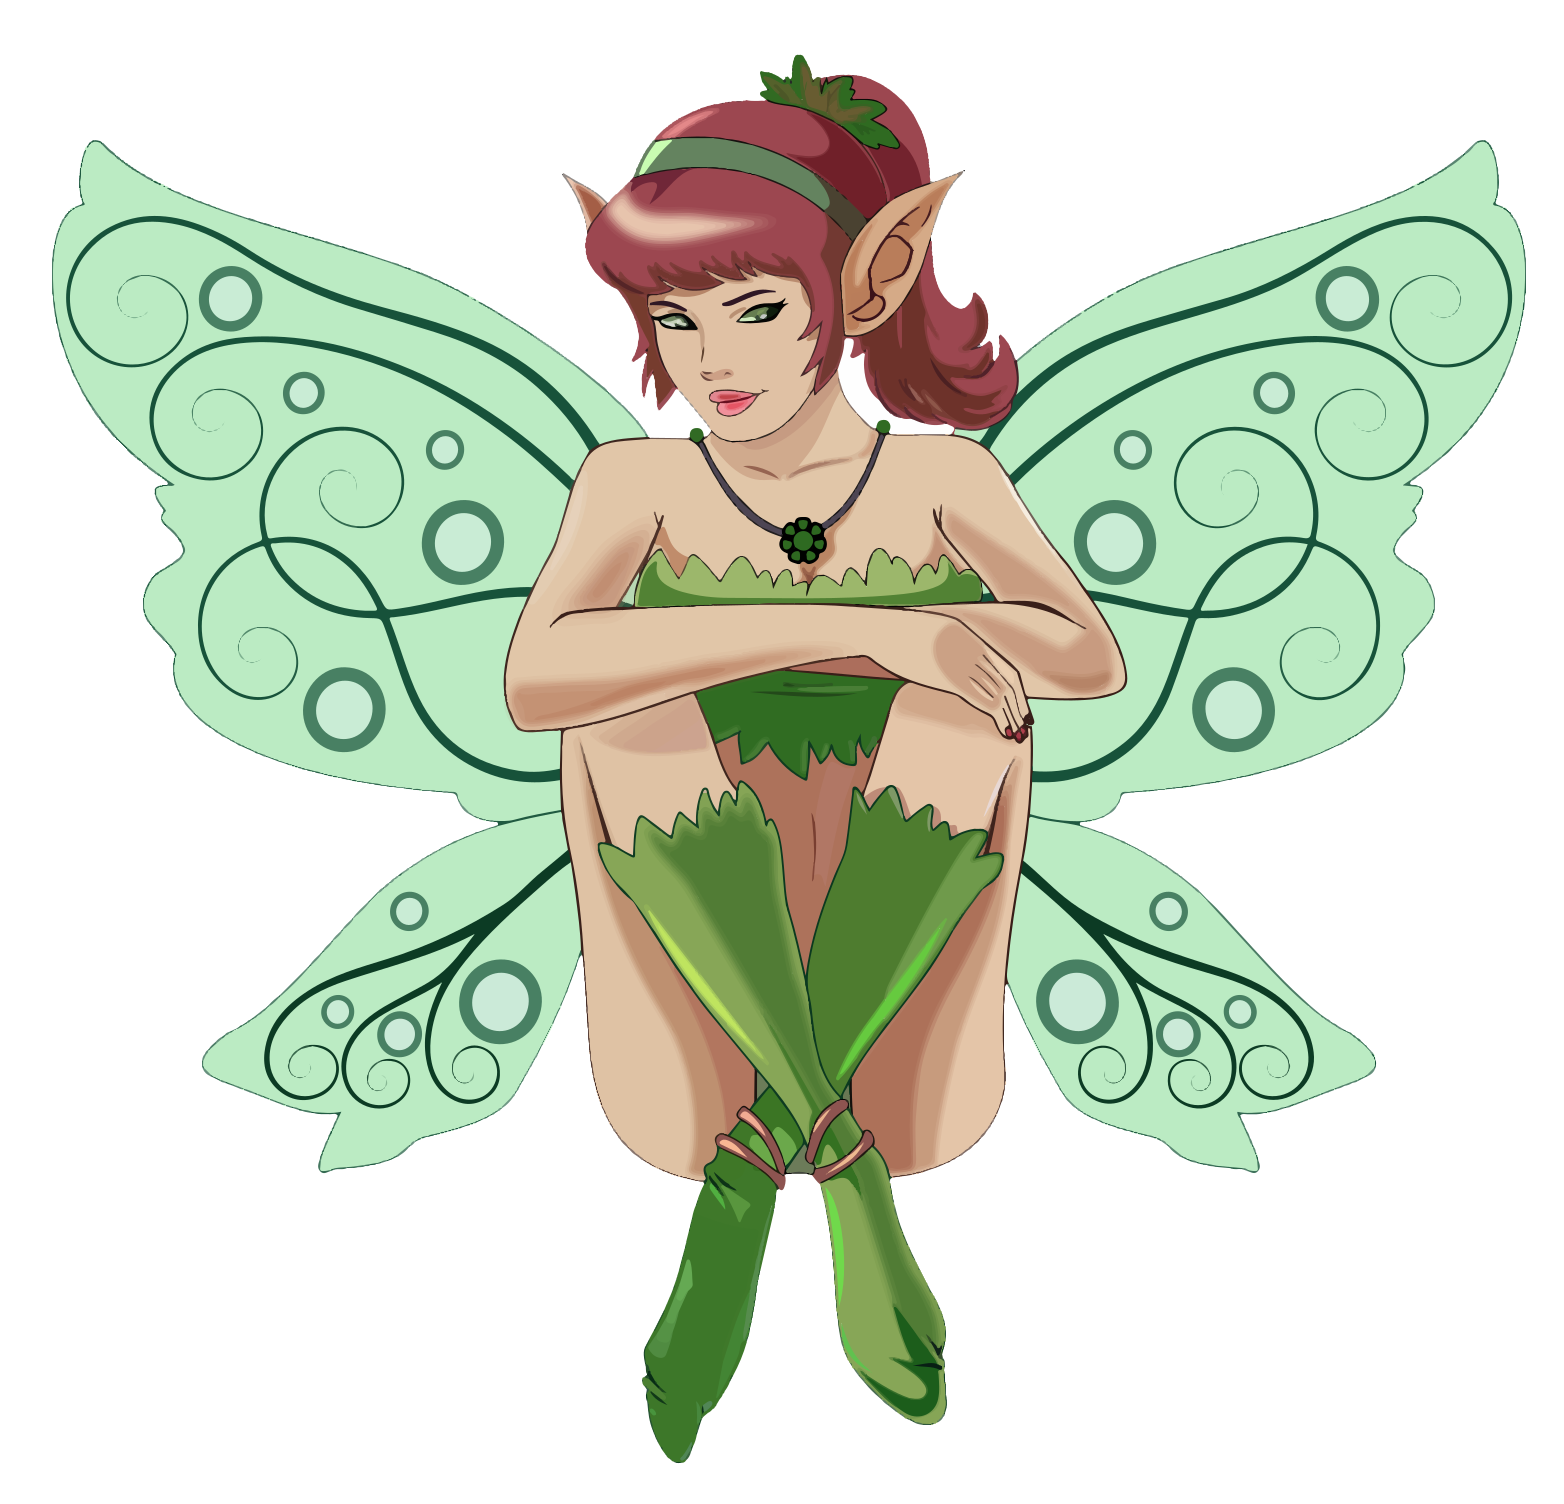
\includegraphics[width=\columnwidth]{Monsters/Faerie}

\subsection{Faun}\index[monsters]{Faun}
\statblock{\textbf{Size:} Medium

\textbf{Type:} Humanoid

\textbf{Habitat:} Underground, Woods (Rare)

\textbf{Wandering Group:} 1d12 (A)

\textbf{Lair Group:} 0 (Nil)

\textbf{Move:} 50 ft.

\textbf{Armor Class:} 7

\textbf{Hit Dice:} 1/2 (2 HP)

\textbf{Attacks:} Weapon (By weapon)

\textbf{Special:} None

\textbf{Save:} R1

\textbf{Alignment:} Chaotic

\textbf{Intelligence:} 

\textbf{Morale:} 6

\textbf{XP Value:} 5}

Fauns are male human-sized wood spirits that are a combination of man and beast. Their legs are those of a goat, horse, or any other similar animal, and their torso is that of a human. They have two small horns extruding from their forehead and ears that match the aforementioned animal's ears. Fauns usually don't wear any clothing, but may be found wearing various types of jewelry.

Fauns are kind-hearted, impulsive and unpredictable; they suffer from mood swings. They are big fans of dancing and music and can usually be found carrying an instrument with which they are proficient in playing.

\subsubsection{Spellcasting}
Fauns can be shamans (to \nth{7} level).

\subsubsection{As a Class}\index[classes]{Faun}
Fauns can be used as a class using the following statistics:

\textbf{Musical Instrument:} Fauns begin play with a musical instrument of their choice. The faun is considered an expert of the chosen instrument. This expertise allows the faun to repair the instrument or build a new one as long as the materials are available to him.

When a faun reaches \nth{5} level, he is able to use his musical instrument to effect a creature's emotions. By playing his instrument for a full round, the faun may attempt to draw out and amplify an emotion from a creature, causing that creature to be entirely focused on the effected emotion. The creature can avoid this effect with a successful saving throw vs. spells with a +4 bonus. Each additional round the faun plays and each level above 5 the faun has attained, this bonus is reduced by 1, eventually becoming a penalty. If the faun plays too long, he may become susceptible to his own effect. On the fifth round and each round thereafter, the faun must succeed at a saving throw vs, spells, or fall victim to his own effect. If the faun's playing is interrupted, he must start over as if it was the first round.

When a faun reaches level 10, he is able to use his musical instrument to effect the growth of plants. By playing his instrument for 5 rounds or more, the faun causes plants to grow as the Growth of Plants spell.

\statblock{\textbf{Ability Requirements:} Strength 6, Dexterity 8, Constitution 7

\textbf{Prime Requisite:} Dexterity

\textbf{Ability Modifiers:} Dexterity +1, Constitution -1

\textbf{Weapons:} Any

\textbf{Armor:} Any Custom (2x Cost)

\textbf{Natural AC:} 8

\textbf{Special Abilities:} Musical Instrument

\textbf{Magic Item Use:} All except Wizard}

\begin {table}[H]
  \caption{Faun Progression}
  \begin{tabularx}{\columnwidth}{>{\bfseries}YYY}
	\thead{Level} & \thead{Experience} & \thead{Hit Dice}\\
	0 & 0 & 1d4\\
	1 & 1,000 & 2d4\\
	2 & 2,000 & 3d4\\
	3 & 4,000 & 4d4\\
	4 & 8,000 & 5d4\\
	5 & 16,000 & 6d4\\
	6 & 32,000 & 7d4\\
	7 & 64,000 & 8d4\\
	8 & 130,000 & 9d4\\
	9 & 260,000 & 10d4\\
	10+ & +200,000 & +2 HP
  \end {tabularx}
\end {table}

\subsection{Ferret, Giant}\index[monsters]{Giant Ferret}
\statblock{\textbf{Size:} Small

\textbf{Type:} Animal

\textbf{Habitat:} Woods (Common)

\textbf{Wandering Group:} 1d8 (Nil)

\textbf{Lair Group:} 1d12 (Nil)

\textbf{Move:} 50 ft.

\textbf{Armor Class:} 5

\textbf{Hit Dice:} 1+1 (6 HP)

\textbf{Attacks:} Bite (1d8)

\textbf{Special:} None

\textbf{Save:} F1

\textbf{Alignment:} None

\textbf{Intelligence:} 2

\textbf{Morale:} 8

\textbf{XP Value:} 15}

Giant ferrets are slender mammals with brown or creamy fur.

Giant ferrets are inquisitive and friendly creatures, that are generally omnivorous (although they particularly like eating giant rats). However, if not treated well they rapidly become frustrated and angry, and this makes them less suitable as companion animals or pets.

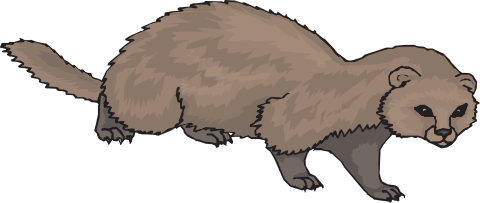
\includegraphics[width=\columnwidth]{Monsters/Animals/Ferret, Giant}

\subsection{Firebird}\index[monsters]{Firebird}
\statblock{\textbf{Size:} Large

\textbf{Type:} Monster

\textbf{Habitat:} Void (Rare)

\textbf{Wandering Group:} 0 (Nil)

\textbf{Lair Group:} 1d2 (V)

\textbf{Move:} 30 ft., 120 ft. (Fly)

\textbf{Armor Class:} 2*

\textbf{Hit Dice:} 9**** (81 HP)

\textbf{Attacks:} 2x Claw (1d6) \& Bite (2d6)

\textbf{Special:} Explode, Halo of Fire, 

Immunity (Charm, Fire, Hold, Weapons < +2), Regeneration (5)

\textbf{Save:} F10

\textbf{Alignment:} Neutral

\textbf{Intelligence:} 6

\textbf{Morale:} 10

\textbf{XP Value:} 3,700}

Firebirds are lesser cousins of phoenixes that appear as red-orange eagle-like birds. They have bright white-blue eyes and are surrounded by a halo of fire. Firebirds are never hostile unless attacked, but will fight to the death to defend themselves.

\textbf{Explode:} If a firebird is destroyed, it explodes into a 9d6 Fireball with a 20-foot radius. Creatures in the area may save vs. breath weapon to take half damage, but resistances or immunities to fire do not reduce the damage.

\textbf{Halo of Fire:} All creatures within 10 feet of a firebird take 3d6 fire damage per round.

\includegraphics[width=\columnwidth]{Monsters/Firebird}

\subsection{Fish, Giant Bass}\index[monsters]{Giant Bass}
\statblock{\textbf{Size:} Large

\textbf{Type:} Animal

\textbf{Habitat:} Ocean, River (Common)

\textbf{Wandering Group:} 0 (Nil)

\textbf{Lair Group:} 2d4 (Nil)

\textbf{Move:} 40 ft. (Swim)

\textbf{Armor Class:} 7

\textbf{Hit Dice:} 2 (9 HP)

\textbf{Attacks:} Bite (1d6)

\textbf{Special:} None

\textbf{Save:} F1

\textbf{Alignment:} None

\textbf{Intelligence:} 1

\textbf{Morale:} 8

\textbf{XP Value:} 20}

Giant bass are common in rivers, although they are rarely aggressive against creatures larger than a halfling.

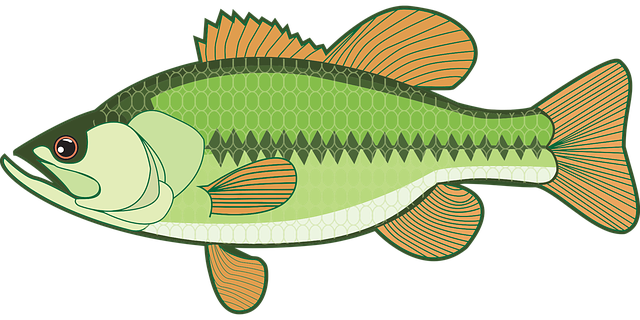
\includegraphics[width=\columnwidth]{Monsters/Animals/Fish, Giant Bass}

\subsection{Fish, Giant Stone}\index[monsters]{Giant Stone Fish}
\statblock{\textbf{Size:} Large

\textbf{Type:} Animal

\textbf{Habitat:} Ocean, River (Common)

\textbf{Wandering Group:} 0 (Nil)

\textbf{Lair Group:} 2d4 (Nil)

\textbf{Move:} 60 ft. (Swim)

\textbf{Armor Class:} 7

\textbf{Hit Dice:} 5+5* (28 HP)

\textbf{Attacks:} Spine (1d4)

\textbf{Special:} Poison

\textbf{Save:} F3

\textbf{Alignment:} None

\textbf{Intelligence:} 1

\textbf{Morale:} 8

\textbf{XP Value:} 400}

Stonefish are spiked fish that look remarkably like rocks and coral when still. There is a 70\% chance of such misidentification.

They hunt by waiting in ambush and then snapping at other small fish, and will not attack larger creatures.

However, anyone who stands on the “rock” that is actually the stonefish will be automatically struck by four of the fish’s poisonous spines.

If pressed and unable to escape, the fish will actively try to hit a target with one of its spines at normal to-hit chances.

\textbf{Poison:} Anyone struck by one of the stonefish's spines must make a saving throw vs. poison or die.

\subsection{Fish, Giant Sturgeon}\index[monsters]{Giant Sturgeon}
\statblock{\textbf{Size:} Large

\textbf{Type:} Animal

\textbf{Habitat:} Ocean, River (Rare)

\textbf{Wandering Group:} 0 (Nil)

\textbf{Lair Group:} 2d10 (Nil)

\textbf{Move:} 60 ft. (Swim)

\textbf{Armor Class:} 0

\textbf{Hit Dice:} 10+2 (47 HP)

\textbf{Attacks:} Bite (2d10)

\textbf{Special:} Swallow Whole

\textbf{Save:} F5

\textbf{Alignment:} None

\textbf{Intelligence:} 1

\textbf{Morale:} 9

\textbf{XP Value:} 1,900}

Giant sturgeons are aggressive fish which will attack swimmers.

\textbf{Swallow Whole:} If a giant sturgeon hits an opponent of human size or smaller with a natural roll of 18 or better, the opponent is swallowed. Swallowed opponents take 2d6 damage per round, and must make a saving throw vs. death each round to be able to attack the fish from the inside for that round.

\subsection{Gargoyle}\index[monsters]{Gargoyle}
\statblock{\textbf{Size:} Medium

\textbf{Type:} Construct

\textbf{Habitat:} Underground (Rare)

\textbf{Wandering Group:} 1d6 (Nil)

\textbf{Lair Group:} 2d4 (C)

\textbf{Move:} 30 ft., 50 ft. (Fly)

\textbf{Armor Class:} 5*

\textbf{Hit Dice:} 4** (18 HP)

\textbf{Attacks:} 2x Claw (1d3) \& 

Bite (1d6) \& Horn (1d4)

\textbf{Special:} Immunity (Mind Effects, Normal Weapons, Poison)

\textbf{Save:} F8

\textbf{Alignment:} Chaotic

\textbf{Intelligence:} 5

\textbf{Morale:} 11

\textbf{XP Value:} 175}

Of all the types of construct, gargoyles are the most intelligent and the most prone to gaining free will if left without an owner.

A gargoyle is usually made of stone and looks like a winged and horned humanoid figure. Despite their weight, they can fly clumsily yet quickly.

Because gargoyles are usually created as guards, they are prone to be very territorial when rogue, attacking anyone who approaches their lair.

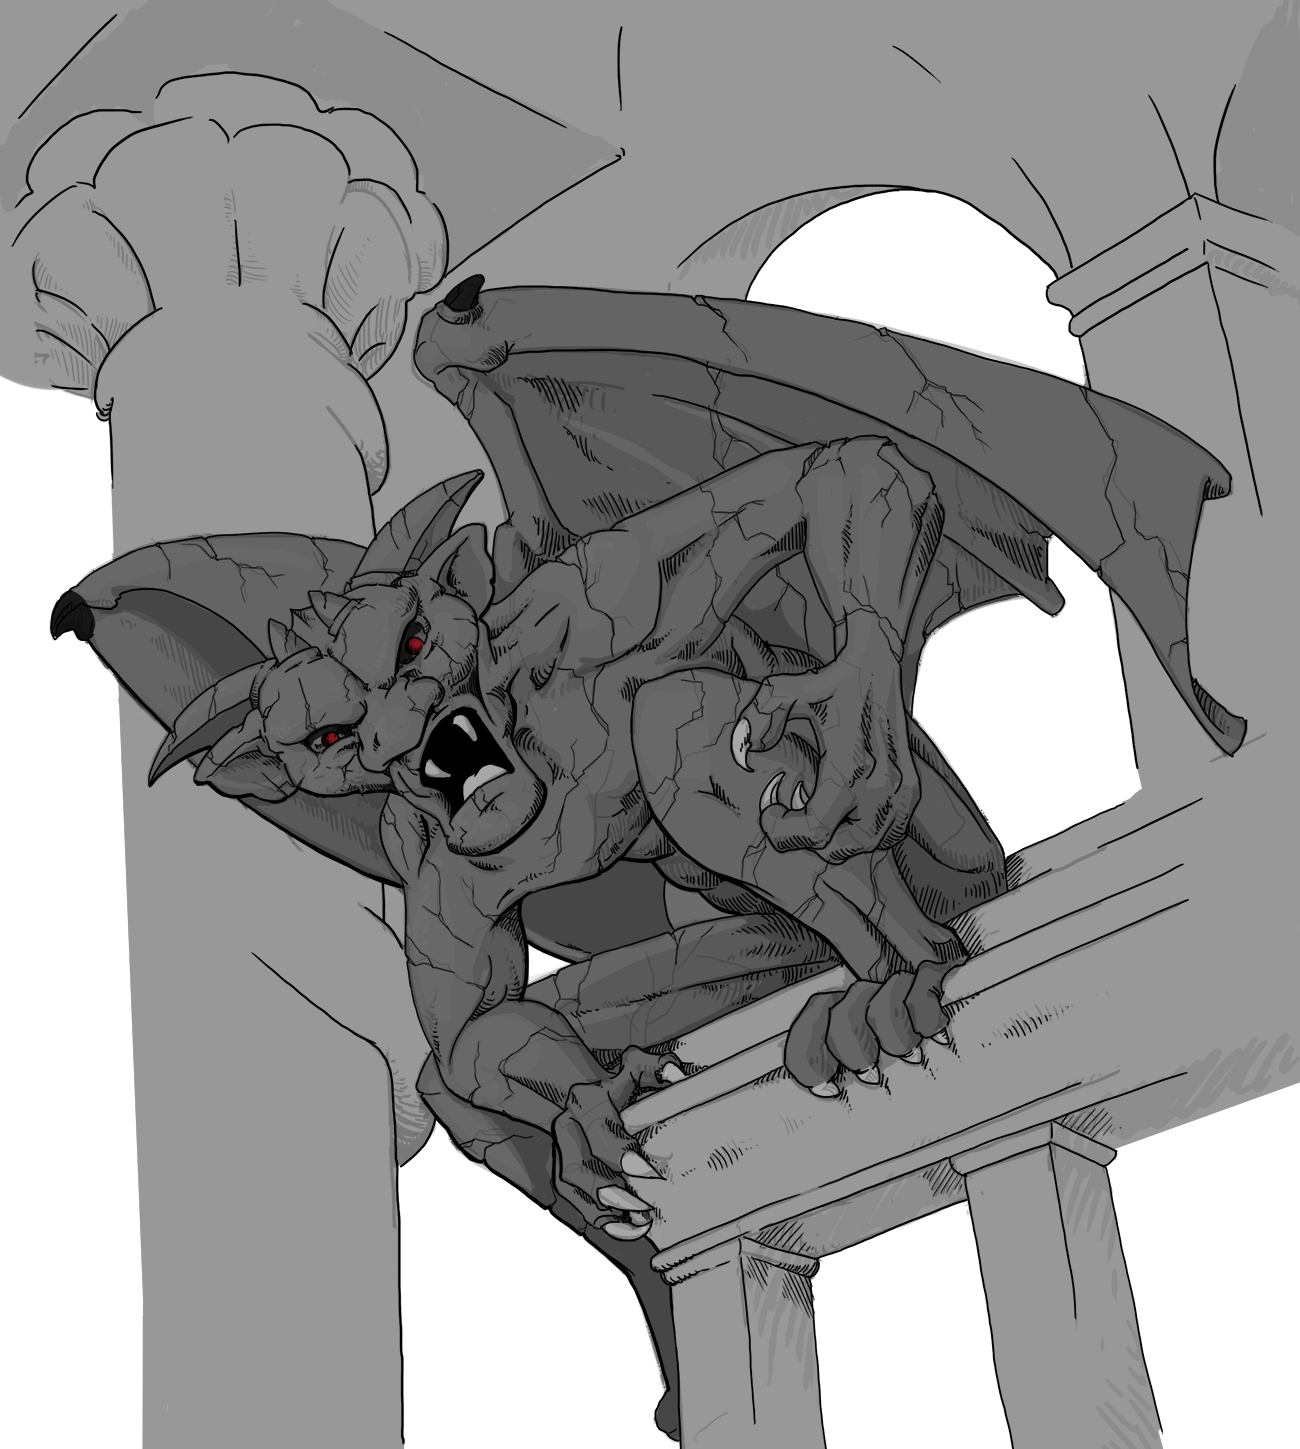
\includegraphics[width=\columnwidth]{Monsters/Gargoyle}

\subsection{Gazer}\index[monsters]{Gazer}
\statblock{\textbf{Size:} Medium

\textbf{Type:} Monster

\textbf{Habitat:} Underground (Rare)

\textbf{Wandering Group:} 0 (Nil)

\textbf{Lair Group:} 1 (L, N, O)

\textbf{Move:} 10 ft.

\textbf{Armor Class:} 0 (Body), 2 (Beak), 7 (Tentacles)

\textbf{Hit Dice:} 11***** (Body: 50 HP, 

Beak 20 HP, Tentacles 12 HP each)

\textbf{Attacks:} Bite (2d6)

\textbf{Special:} Anti-Magic, Spell-like Abilities

\textbf{Save:} W11

\textbf{Alignment:} Chaotic

\textbf{Intelligence:} 16

\textbf{Morale:} 12

\textbf{XP Value:} 5,100}

A gazer is a strange creature. It consists of ten tentacles in a rough ball shape. Each tentacle ends with lip-less mouth, and there is another beak-like mouth in the center of the creature. A gazer has no visible eyes or means of locomotion, although it is able to see and able to levitate and fly. The flight of a gazer is not magical, and is not affected by Anti-Magic or any kind of dispel.

Gazers are domineering creatures who seem to delight in power over others for its own sake. A gazer can speak in a multitude of simultaneous voices, but will rarely do so other than to order minions about.

Although a gazer can bite with its main mouth, its main attacks are the rays that it can project from its various mouths.

When attacking a gazer, a character can choose to attack the body, the beak, or a tentacle.

Removing all the hit points from the body will kill the gazer.

Removing all the hit points from the beak will prevent the gazer from using its Anti-Magic but will not kill it.

Removing all the hit points from one tentacle will prevent the gazer from using that tentacle’s spell like effect. However, attacks targeting tentacles will always hit a random tentacle.

Area effect attacks will always do damage to the body.

\textbf{Anti-Magic:} The main mouth projects an Anti-Magic effect to a range of 60 feet in front of the creature.

\textbf{Spell-like Abilities:} The lesser mouths of an undead gazer can project the following effects: \iref[spell:Charm Person]{Charm Person}, \iref[spell:Charm Monster]{Charm Monster}, \iref[spell:Sleep]{Sleep}, \iref[spell:Telekinesis]{Telekinesis}, \ilink{spell:Flesh to Stone}{Flesh to Stone}, \iref[spell:Disintegrate]{Disintegrate}, \ilink{spell:Cause Fear}{Cause Fear}, \ilink{spell:Slow}{Slow}, \ilink{spell:Cause Serious Wounds}{Cause Serious Wounds}, and \iref[spell:Death Spell]{Death Spell}.

Each mouth can project its spell once per round, although even by twisting its body, a gazer can only get a maximum of four mouths to point at any given target at once. None of the spell effects from the lesser mouths can affect creatures directly in front of the gazer, since the Anti-Magic ray from its main mouth suppresses them.

\subsection{Gazer, Undead}\index[monsters]{Undead Gazer}
\statblock{\textbf{Size:} Medium

\textbf{Type:} Undead, Monster

\textbf{Habitat:} Underground (Very Rare)

\textbf{Wandering Group:} 0 (Nil)

\textbf{Lair Group:} 1 (Lx2,Nx2,Ox2)

\textbf{Move:} 20 ft.

\textbf{Armor Class:} -4 (Body), -2 (Beak), 3 (Tentacles)

\textbf{Hit Dice:} 20******* (Body: 90 HP, Beak: 30 HP, Tentacles: 20 HP each)

\textbf{Attacks:} Bite (2d10)

\textbf{Special:} Cone of Reflection, Gaseous Form, 

Immunity (Death Rays, Illusion, Mind Effects, Poison), 

Regeneration (3), Spell-like Abilities

\textbf{Save:} W20

\textbf{Alignment:} Chaotic

\textbf{Intelligence:} 16

\textbf{Morale:} 12

\textbf{XP Value:} 14,975}

It is not known how gazers become undead, but they can do so—and the result is even more horrific.

An undead gazer can only be hit by +2 weapons or better.

An undead gazer is turned as if a Nightshade.

When attacking an undead gazer, a character can choose to attack the body, the beak, or a tentacle.

Removing all the hit points from the body will force the undead gazer into Gaseous Form until it can rest in complete darkness for at least one hour. Any further damage done to the undead gazer during this time (which can only be done by spells that affect air) will kill it.

Removing all the hit points from the beak will prevent the undead gazer from using its Reflection ability but will not kill it.

Removing all the hit points from one tentacle will prevent the undead gazer from using that tentacle’s spell like effect. However, attacks targeting tentacles will always hit a random tentacle.

Area effect attacks will always do damage to the body.

\textbf{Gaseous Form:} An undead gazer can turn into gaseous form at will, in which state it can not attack or use its spell like abilities but it can only be hurt by magical abilities that affect air.

\textbf{Reflection:} The main beak of an undead gazer projects a cone of reflection. Any spell or Turn Undead attempt that is cast within this cone will be reflected back on its caster.

In the case of Turn Undead attempts, the turning cleric must make a saving throw vs. spells or flee in terror for 2d6 rounds.

\textbf{Spell-like Abilities:} The lesser mouths of an undead gazer can project the following effects: \iref[spell:Animate Dead]{Animate Dead}, \iref[spell:Charm Monster]{Charm Monster}, \ilink{spell:Continual Darkness}{Continual Darkness}, \iref[spell:Death Spell]{Death Spell}, \ilink{spell:Energy Drain}{Energy Drain} (1 level), \ilink{spell:Energy Drain}{Energy Drain} (2 levels), Paralysis (as a ghoul), \iref[spell:Animate Objects]{Animate Objects}, \iref[spell:Dispel Magic]{Dispel Magic}, and \iref[spell:Telekinesis]{Telekinesis}.

Each mouth can project its spell once per round, although even by twisting its body, an undead gazer can only get a maximum of four mouths to point at any given target at once. None of the spell effects from the lesser mouths can affect creatures directly in front of the gazer, since the Anti-Magic ray from its main mouth suppresses them.

\subsection{Gelatinous Cube}\index[monsters]{Gelatinous Cube}
\statblock{\textbf{Size:} Large

\textbf{Type:} Ooze

\textbf{Habitat:} Underground (Common)

\textbf{Wandering Group:} 1 (V)

\textbf{Lair Group:} 0 (Nil)

\textbf{Move:} 20 ft.

\textbf{Armor Class:} 8*

\textbf{Hit Dice:} 4* (18 HP)

\textbf{Attacks:} Touch (2d4)

\textbf{Special:} Immunity (Cold, Lightning), 

Paralyzing Touch, Wall of Ooze

\textbf{Save:} F2

\textbf{Alignment:} None

\textbf{Intelligence:} 0

\textbf{Morale:} 12

\textbf{XP Value:} 125}

A gelatinous cube is exactly what the name implies, a large blob of transparent oozing slime. Although not naturally cubic, these oozes feed by scraping detritus from the floor, walls and ceiling, and therefore often end up in a cubic shape as they press into the corners of a corridor.

A gelatinous cube will attack any creatures it encounters with it's paralyzing touch. The cube will keep attacking until either it is dead or all enemies are dead.

Although unintelligent, a gelatinous cub will often have bits of indigestible treasure embedded in it.

\textbf{Engulf:} If all the gelatinous cube's enemies are incapacitated, the cube will roll over the victims and start digesting them.

\textbf{Paralyzing Touch:} Anyone touched by a gelatinous cube must make a saving throw vs. paralyzation or be paralyzed for 2d4x10 minutes.

\textbf{Wall of Ooze:} When filling a corridor, gelatinous cubes are often hard to see, and surprise opponents on a roll of 1-4 on a d6.

\subsection{Ghast}\index[monsters]{Ghast}
\statblock{\textbf{Size:} Medium

\textbf{Type:} Undead

\textbf{Habitat:} Barren Land, Clear, Underground (Very Rare)

\textbf{Wandering Group:} 1d6 (Nil)

\textbf{Lair Group:} 1d10 (C)

\textbf{Move:} 40 ft.

\textbf{Armor Class:} 6

\textbf{Hit Dice:} 3** (14 HP)

\textbf{Attacks:} 2x Claw (1d3 + Paralyze) 

or Weapon (By weapon)

\textbf{Special:} Immunity (Mind Effects, Poison), 

Paralysis, Regeneration (1)

\textbf{Save:} F3

\textbf{Alignment:} Chaotic

\textbf{Intelligence:} 6

\textbf{Morale:} 10

\textbf{XP Value:} 65}

A ghast is a stronger, quicker and more dangerous version of a ghoul. 

Ghasts are turned as if they are Wights.

Ghasts look just like ghouls, and have been known to lead packs of ghouls due to their intelligence.

Although ghasts have more intelligence than ghouls and more memories of when they were alive, they are still primarily motivated by hunger, and still do not speak.

Their constant hunger compels them to kill and eat, although they have been seen to show remorse for their actions, and can sometimes be found wailing and crying at their fate.

\textbf{Paralysis:} Any ogre-sized or smaller creature touched by a ghast must make a saving throw vs. paralysis or be paralyzed for 2d4x10 minutes. Elves are immune to this paralysis.

\subsection{Ghoul}\index[monsters]{Ghoul}
\monsterimage[.2]{Monsters/Ghoul}{\statblock{\textbf{Size:} Medium

\textbf{Type:} Undead

\textbf{Habitat:} Underground (Common)

\textbf{Wandering Group:} 1d6 (Nil)

\textbf{Lair Group:} 2d8 (B)

\textbf{Move:} 30 ft.

\textbf{Armor Class:} 6

\textbf{Hit Dice:} 2* (9 HP)

\textbf{Attacks:} 2x Claw (1d3 + 

Paralyze) \& Bite (1d3 + Paralyze)

\textbf{Special:} Immunity 

(Mind Effects, Poison), Paralysis

\textbf{Save:} F2

\textbf{Alignment:} None

\textbf{Intelligence:} 3

\textbf{Morale:} 9

\textbf{XP Value:} 25}}

A ghoul is an undead creature that eats carrion and rotten meat. As an undead, they are immune to Sleep and Charm spells.

Ghouls look like zombies when standing still, although they are much more agile, capable of climbing and running at full speed.

Ghouls have a level of animal cunning approximately equal to that of dogs, although they have only vague memories of their lives and they cannot speak.

A ghoul’s normal hunting tactic is to ignore paralyzed opponents until there are no more moving ones left, and then kill all the paralyzed victims and leave their corpses to rot into an edible state.

\textbf{Paralysis:} Any ogre-sized or smaller creature touched by a ghoul must make a saving throw vs. paralysis or be paralyzed for 2d4x10 minutes. Elves are immune to this paralysis.

\subsection{Giant, Cloud}\index[monsters]{Cloud Giant}
\statblock{\textbf{Size:} Large

\textbf{Type:} Giant

\textbf{Habitat:} Mountains (Rare)

\textbf{Wandering Group:} 1d2 (Nil)

\textbf{Lair Group:} 1d3 (E+5,000 gp)

\textbf{Move:} 40 ft.

\textbf{Armor Class:} 4

\textbf{Hit Dice:} 13*** (59 HP)

\textbf{Attacks:} Weapon (By weapon)

\textbf{Special:} Keen Senses, Rock Throwing

\textbf{Save:} F12

\textbf{Alignment:} Neutral

\textbf{Intelligence:} 16

\textbf{Morale:} 10

\textbf{XP Value:} 4,200}

Cloud giants are fierce and territorial humanoids with white skin and hair and keen senses. They live on top of mountains above the cloud line, and often keep small rocs (1d6) or dire wolves (6d6) as pets.

Cloud giants tend to be loners, and dislike being disturbed—although they don’t automatically attack intruders into their territory they will usually hint strongly that such intruders should leave as soon as they are able.

\textbf{Keen Senses:} Cloud giants have keen senses, and are only surprised on a roll of 1 on 1d6.

\textbf{Rock Throwing:} Cloud giants can throw rocks (range: 60/130/200) at opponents who are outside melee range. A successful attack inflict 3d6 damage.

\subsubsection{Spellcasting}
Cloud giants can be shamans (to \nth{10} level) or sorcerers (to \nth{10} level).

\subsubsection{Giant, Fire}\index[monsters]{Fire Giant}
\statblock{\textbf{Size:} Large

\textbf{Type:} Giant

\textbf{Habitat:} Jungle (Rare)

\textbf{Wandering Group:} 1d2 (Nil)

\textbf{Lair Group:} 1d3 (E+5,000 gp)

\textbf{Move:} 40 ft.

\textbf{Armor Class:} 4

\textbf{Hit Dice:} 11+2*** (52 HP)

\textbf{Attacks:} Weapon (By weapon)

\textbf{Special:} Rock Throwing

\textbf{Save:} F11

\textbf{Alignment:} Chaotic

\textbf{Intelligence:} 13

\textbf{Morale:} 19

\textbf{XP Value:} 3,875}

Fire giants are humanoids with dark red skin and black hair. They live in or near volcanoes, and are immune to fire and fire based attacks. Fire giants usually keep hydras (1d3) or hellhounds (3d6) as pets.

Fire giants love to fight and make war, usually against their frost giant rivals, but often against each other. When not actually fighting, fire giants show great hospitality, carousing and partying with visitors and guests.

Fire giants are excellent blacksmiths, and will often trade metal goods—particularly arms and armor—with their neighbors when not at war with them.

\textbf{Rock Throwing:} Fire giants can throw rocks (range: 60/130/200) at opponents who are outside melee range. A successful attack inflict 3d6 damage.

\subsubsection{Spellcasting}
Fire giants can be shamans (to \nth{8} level) or sorcerers (to \nth{6} level).

\subsection{Giant, Frost}\index[monsters]{Frost Giant}
\statblock{\textbf{Size:} Large

\textbf{Type:} Giant

\textbf{Habitat:} Arctic (Rare)

\textbf{Wandering Group:} 1d2 (Nil)

\textbf{Lair Group:} 1d4 (E+5,000 gp)

\textbf{Move:} 40 ft.

\textbf{Armor Class:} 4

\textbf{Hit Dice:} 10+2** (46 HP)

\textbf{Attacks:} Weapon (By weapon)

\textbf{Special:} Immunity to Cold, Rock Throwing

\textbf{Save:} F10

\textbf{Alignment:} Chaotic

\textbf{Intelligence:} 14

\textbf{Morale:} 9

\textbf{XP Value:} 3,875}

Frost giants are humanoids with pale blue skin and white or yellow hair. They live in mountains above the snow line and in polar regions, and are immune to cold and cold based attacks. Frost giants usually keep polar bears (3d6) or wolves (6d6) as pets.

Frost giants try to be empire builders, dominating all the other races in their area. Providing visitors show the deference that they think is due to them, frost giants are welcoming. They love to show off their prestige and power.

\textbf{Rock Throwing:} Frost giants can throw rocks (range: 60/130/200) at opponents who are outside melee range. A successful attack inflict 3d6 damage.

\subsubsection{Spellcasting}
Frost giants can be shamans (to \nth{8} level) or sorcerers (to \nth{6} level).

\subsection{Giant, Hill}\index[monsters]{Hill Giant}
\statblock{\textbf{Size:} Large

\textbf{Type:} Giant

\textbf{Habitat:} Hills, Mountains (Common)

\textbf{Wandering Group:} 1d4 (Nil)

\textbf{Lair Group:} 1d4 (E+5,000 gp)

\textbf{Move:} 40 ft.

\textbf{Armor Class:} 4

\textbf{Hit Dice:} 8* (36 HP)

\textbf{Attacks:} Weapon (By weapon)

\textbf{Special:} Rock Throwing

\textbf{Save:} F8

\textbf{Alignment:} Chaotic

\textbf{Intelligence:} 7

\textbf{Morale:} 8

\textbf{XP Value:} 1,200}

Hill giants are hairy and rather dim witted. They live in roughly made cottages in hills or at the base of mountains. They tend to wear animal skins and use natural weapons such as clubs and spears.

Hill giants are cantankerous and belligerent, and often take to minor banditry or raiding, since they haven’t the patience for farming and herding.

However, they love flattery and tributes (particularly of alcohol); and this will often keep them pacified and away from trouble.

\textbf{Rock Throwing:} Hill giants can throw rocks (range: 30/60/100) at opponents who are outside melee range. A successful attack inflict 3d6 damage.

\subsubsection{Spellcasting}
Hill giants can be shamans (to \nth{8} level) or sorcerers (to \nth{6} level).

\subsection{Giant, Sea}\index[monsters]{Sea Giant}
\statblock{\textbf{Size:} Large

\textbf{Type:} Giant

\textbf{Habitat:} Ocean (Rare)

\textbf{Wandering Group:} 1d2 (Nil)

\textbf{Lair Group:} 1d20 (E+5,000 gp)

\textbf{Move:} 40 ft., 40 ft. (Swim)

\textbf{Armor Class:} 0

\textbf{Hit Dice:} 12 (54 HP)

\textbf{Attacks:} Weapon (By weapon)

\textbf{Special:} Aquablast, Hold Breath, Rock Throwing

\textbf{Save:} F12

\textbf{Alignment:} Neutral

\textbf{Intelligence:} 12

\textbf{Morale:} 10

\textbf{XP Value:} 2,125}

Sea giants appear like normal humans, except they stand between 15 and 20 feet tall. They live in the deepest canyons of the ocean depths and are normally friendly when encountered.

\textbf{Aquablast:} Sea giants can push water with tremendous force, creating a 50-feet long 3-feet wide cone-shaped underwater current that shoves anyone in its path 60 feet away. All victims are swept away at great speed and must make a saving throw vs. death ray or become \iref[sec:Stunned]{Stunned} for 1d6 rounds.

This ability can also be used to create a tidal wave above water with the same effect, but the area of effect is 120-feet long and 60-feet wide. All vessels in the path of the tidal wave suffer 2d6 points of hull damage

\textbf{Hold Breath:} Sea giants can not breathe air, but they can hold their breath for up to 10 minutes.

\textbf{Rock Throwing:} Sea giants can throw rocks (range: 100/200/400) at opponents who are outside melee range. A successful attack inflict 3d6 damage.

\subsubsection{Spellcasting}
Sea giants can be shamans (to \nth{4} level) or sorcerers (to \nth{10} level).

\subsubsection{As a Class}\index[classes]{Sea Giant}
Sea giants can be used as a class using the following statistics:

\textbf{Aquablast:} This ability is not gained until level 0.

\textbf{Damage Bonus:} Beginning at level 0, sea giants gain a +2 damage bonus to all attacks.

\textbf{Hold Breath:} Sea giants can hold their breath for a number of minutes equal to their Constitution score.

\statblock{\textbf{Ability Requirements:} Strength 15

\textbf{Prime Requisite:} Strength, Dexterity, Intelligence, or Wisdom

\textbf{Ability Modifiers:} Strength +2, Dexterity -2

\textbf{Weapons:} Any

\textbf{Natural Attacks:} Fist: 1d3 (Level -9), 1d6 (Level -8), 1d8 (Level -6), 2d6 (Level -4), 2d8 (Level -2), 3d6 (Level 0+)

\textbf{Armor:} Any

\textbf{Natural AC:} 9 (Level -9), -1 per level (Level -8 to 0)

\textbf{Special Abilities:} Create Current, Damage Bonus, Hold Breath, Rocking Throwing

\textbf{Magic Item Use:} Fighter}

\begin {table}[H]
  \caption{Sea Giant Progression}
  \begin{tabularx}{\columnwidth}{>{\bfseries}YYY}
	\thead{Level} & \thead{Experience} & \thead{Hit Dice}\\
	-9 & -400,000 & 4d8\\
	-8 & -395,000 & -\\
	-7 & -385,000 & 5d8\\
	-6 & -370,000 & -\\
	-5 & -352,000 & 6d8\\
	-4 & -327,000 & -\\
	-3 & -294,000 & 7d8\\
	-2 & -252,000 & -\\
	-1 & -200,000 & 8d8\\
	0 & 0 & 9d8\\
	1 & 400,000 & -\\
	2 & 700,000 & 10d8\\
	3 & 1,000,000 & -\\
	4 & 1,300,000 & 11d8\\
	5 & 1,600,000 & -\\
	6 & 1,900,000 & 12d8\\
	7 & 2,200,000 & -\\
	8 & 2,500,000 & 13d8\\
	9 & +300,000 & +2 HP
  \end {tabularx}
\end {table}

\subsection{Giant, Stone}\index[monsters]{Stone Giant}
\statblock{\textbf{Size:} Large

\textbf{Type:} Giant

\textbf{Habitat:} Underground (Rare)

\textbf{Wandering Group:} 1d2 (Nil)

\textbf{Lair Group:} 1d6 (E+5,000 gp)

\textbf{Move:} 40 ft.

\textbf{Armor Class:} 4

\textbf{Hit Dice:} 9* (41 HP)

\textbf{Attacks:} Weapon (By weapon)

\textbf{Special:} Rock Throwing

\textbf{Save:} F9

\textbf{Alignment:} Neutral

\textbf{Intelligence:} 10

\textbf{Morale:} 9

\textbf{XP Value:} 1,600}

Stone giants are humanoids with gray skin and no hair. They live in cave systems inside mountains, and often use stalactites as clubs. They often have cave bears (1d4) as pets.

Stone giants are calm and patient, and rarely get involved with outsiders unless provoked. They often mine gems, and show surprising dexterity for their size when it comes to cutting and polishing them.

\textbf{Rock Throwing:} Stone giants can throw rocks (range: 100/200/300) at opponents who are outside melee range. A successful attack inflict 3d6 damage.

\subsubsection{Spellcasting}
Stone giants can be shamans (to \nth{8} level) or sorcerers (to \nth{6} level).

\subsection{Giant, Storm}\index[monsters]{Storm Giant}
\statblock{\textbf{Size:} Large

\textbf{Type:} Giant

\textbf{Habitat:} Mountains, Ocean (Rare)

\textbf{Wandering Group:} 1 (Nil)

\textbf{Lair Group:} 1d3 (E+5,000 gp)

\textbf{Move:} 50 ft.

\textbf{Armor Class:} 2

\textbf{Hit Dice:} 15**** (68 HP)

\textbf{Attacks:} Weapon (By weapon)

\textbf{Special:} Rock Throwing, Summon Storm

\textbf{Save:} F15

\textbf{Alignment:} Lawful

\textbf{Intelligence:} 18

\textbf{Morale:} 10

\textbf{XP Value:} 6,250}

Storm giants are humanoids with bronze skin and red or yellow hair. They live on the highest mountain peaks or deep underwater and keep griffons (2d4) as pets.

Storm giants are cultured and civilized, and tend to be friendly to those who visit them and freely offer advice and wisdom. They rarely get visitors, due to the inaccessible locations they live in.

\textbf{Rock Throwing:} Storm giants can throw rocks (range: 150/300/450) at opponents who are outside melee range, if no lightning is available. A successful attack inflict 3d6 damage.

\textbf{Summon Storm:} Storm giants can summon a storm, taking ten minutes for it to form, and if in a storm (either a summoned one or a natural one) they can throw lightning bolts once per five rounds. Each lightning bolt does damage equal to the giant’s current hit points, but anyone who makes a saving throw vs. spells will take only half damage. Storm giants are immune to lightning and lightning damage.

\subsubsection{Spellcasting}
Storm giants can be shamans (to \nth{10} level) or sorcerers (to \nth{10} level).

\subsection{Giant/Gargantuan Monster}\index[monsters]{Giant/Gargantuan Monster}\label{monster:Giant/Gargantuan Monster}
\begin {table}[H]
	\normalsize
	\begin{tabularx}{\columnwidth}{@{}>{\bfseries}XXX@{}}
	\hiderowcolors
	& \textbf{Giant} & \textbf{Gargantuan}\\
	Size: & 1 size category higher & 2 size categories higher\\
	Type: & Unchanged & Unchanged\\
	Habitat: & Unchanged & Unchanged\\
	Wandering Group: & x1.5 size & x4 size\\
	& & x2 percentage\\
	Lair Group: & x1.5 size & x4 size,\\
	& & x2 percentage\\
	Move: & x1.5 (Round to nearest 10) & x2\\
	Armor Class: & Unchanged & Unchanged\\
	Hit Dice: & x3 & x8\\
	Attacks: & Unchanged (x1.5) & Unchanged (x4)\\
	Special: & Unchanged except Regeneration (x1.5) & Unchanged except Regeneration (x4)\\
	Save: & Intelligent: F(HD); Unintelligent: F(HD)/2 & Intelligent: F(HD); Unintelligent: F(HD)/2\\
	Alignment: & Unchanged & Unchanged\\
	Intelligence: & Unchanged & Unchanged\\
	Morale: & +2 (Max 20) & +5 (Max 20)\\
	XP Value: & Recalculate & Recalculate\\
	\showrowcolors
  \end {tabularx}
\end {table}

Giant/Gargantuan monsters are larger versions of other monsters.

\subsection{Gnoll}\index[monsters]{Gnoll}
\statblock{\textbf{Size:} Medium

\textbf{Type:} Humanoid

\textbf{Habitat:} Hills, Mountains (Common)

\textbf{Wandering Group:} 1d6 (P)

\textbf{Lair Group:} 3d6 (D)

\textbf{Move:} 30 ft.

\textbf{Armor Class:} 5

\textbf{Hit Dice:} 2

\textbf{Attacks:} Weapon (By weapon + 1)

\textbf{Special:} None

\textbf{Save:} F2

\textbf{Alignment:} Chaotic

\textbf{Intelligence:} 7

\textbf{Morale:} 8

\textbf{XP Value:} 20}

Gnolls are fierce tribal humanoids with furred bodies and the heads (and markings) of hyenas. Gnolls are constantly hungry, and will eat almost anything; including each other.

Gnolls are bullies and respect only strength. They practically never trade, taking whatever weapons and livestock they can steal instead.

While not the brightest of humanoids, they are smart enough to mostly keep away from civilized areas and to keep their raids of such areas to a minimum.

\subsubsection{Spellcasting}
Some exceptional gnolls can become shamans (to \nth{6} level) or sorcerers (to \nth{4} level).

\subsubsection{As a Class}\index[classes]{Gnoll}
Gnolls can be used as a class using the following statistics:

\statblock{\textbf{Ability Requirements:} Strength 13

\textbf{Prime Requisite:} Strength, Dexterity, Intelligence, or Wisdom

\textbf{Ability Modifiers:} Strength +1, Dexterity +1, Wisdom -2

\textbf{Weapons:} Any

\textbf{Armor:} Any

\textbf{Natural AC:} 8

\textbf{Special Abilities:} None

\textbf{Magic Item Use:} Fighter}

\begin {table}[H]
  \caption{Gnoll Progression}
  \begin{tabularx}{\columnwidth}{>{\bfseries}YYYYY}
	\thead{Level} & \thead{Experience} & \thead{Hit Dice}\\
	-1 & -100,000 & 1d8\\
	0 & 0 & 2d8\\
	1 & 1,000 & 3d8\\
	2 & 3,000 & 4d8\\
	3 & 7,000 & -\\
	4 & 15,000 & 5d8\\
	5 & 31,000 & 6d8\\
	6 & 63,000 & 7d8\\
	7 & 129,000 & -\\
	8 & 259,000 & 8d8\\
	9 & 519,000 & 8d8+2\\
	10+ & +300,000 & +2 HP
  \end {tabularx}
\end {table}

\subsection{Gnome}\index[monsters]{Gnome}
\statblock{\textbf{Size:} Small

\textbf{Type:} Humanoid

\textbf{Habitat:} Clear, Underground (Common)

\textbf{Wandering Group:} 1d8 (P)

\textbf{Lair Group:} 5d8 (C)

\textbf{Move:} 20 ft.

\textbf{Armor Class:} 5

\textbf{Hit Dice:} 1 (5 HP)

\textbf{Attacks:} Weapon (By weapon)

\textbf{Special:} As \nth{1} level Gnome

\textbf{Save:} D1

\textbf{Alignment:} Lawful

\textbf{Intelligence:} 11

\textbf{Morale:} 8

\textbf{XP Value:} 10}

Gnomes are humanoids distantly related to dwarves. They look like small humans with long noses and beards but bald heads. Like dwarves, the women have beards like the men.

Gnomes are excellent miners, specializing in mining gems and Red Powder.

Gnomes are excellent tinkerers and inventors, and love anything mechanical. They are very proud of the fact that guns are a gnomish invention.

Unlike their dwarven cousins, gnomes are very magical. They may use any magic item (even those normally only usable by a particular class) and may become shamans (to \nth{12} level) or sorcerers (to \nth{12} level).

\subsection{Goblin}\index[monsters]{Goblin}
\statblock{\textbf{Size:} Small

\textbf{Type:} Humanoid

\textbf{Habitat:} Hills, Mountains, Underground, Woods (Common)

\textbf{Wandering Group:} 2d6 (R)

\textbf{Lair Group:} 6d10 (C)

\textbf{Move:} 30 ft.

\textbf{Armor Class:} 6

\textbf{Hit Dice:} 1-1 (4 HP)

\textbf{Attacks:} Weapon (By weapon)

\textbf{Special:} Infravision, Light Sensitivity

\textbf{Save:} F0

\textbf{Alignment:} Chaotic

\textbf{Intelligence:} 9

\textbf{Morale:} 7

\textbf{XP Value:} 5}

Goblins are green humanoids with pointed ears and noses. They have red eyes that glow softly when there is no light.

Goblins tend to be cowardly, whiny and sniveling, and are easily bullied; but will take every opportunity to be the bullies themselves.

\subsubsection{Spellcasting}
Goblins can make excellent shamans (to level 8) and sorcerers (to level 6). These goblin spellcasters usually rule a goblin tribe by exploiting the fear that the rest of the tribe have of their magic.

\subsubsection{As a Class}\index[classes]{Goblin}
Goblins can be used as a class using the following statistics:

\statblock{\textbf{Ability Requirements:} None

\textbf{Prime Requisite:} Strength, Dexterity, Intelligence, or Wisdom

\textbf{Ability Modifiers:} Strength -3, Dexterity +1, Constitution +1

\textbf{Weapons:} Any

\textbf{Armor:} Any

\textbf{Natural AC:} 8

\textbf{Special Abilities:} None

\textbf{Magic Item Use:} Fighter}

\begin {table}[H]
  \caption{Goblin Progression}
  \begin{tabularx}{\columnwidth}{>{\bfseries}YYY}
	\thead{Level} & \thead{Experience} & \thead{Hit Dice}\\
	0 & 0 & d8-1\\
	1 & 800 & 2d8-2\\
	2 & 1,600 & 3d8-3\\
	3 & 3,200 & -\\
	4 & 6,400 & 4d8-4\\
	5 & 13,000 & 5d8-5\\
	6 & 26,000 & 6d8-5\\
	7 & 55,000 & -\\
	8 & 110,000 & 7d8-5\\
	9 & 220,000 & +2 HP\\
	10+ & +160,000 & +2 HP
  \end {tabularx}
\end {table}

\subsection{Golem}
A golem is an artificial creature created by a high level spellcaster. Golems are made from a specific material used from multiple sources.

\textbf{Immunity to Normal Weapons:} Golems can only be damaged by magical weapons.

\subsubsection{Amber Golem}\index[monsters]{Amber Golem}
\statblock{\textbf{Size:} Large

\textbf{Type:} Construct

\textbf{Habitat:} Any (Rare)

\textbf{Wandering Group:} 1 (Nil)

\textbf{Lair Group:} 1 (Nil)

\textbf{Move:} 60 ft.

\textbf{Armor Class:} 6*

\textbf{Hit Dice:} 10* (45 HP)

\textbf{Attacks:} 2x Claw (2d6) \& Bite (2d10)

\textbf{Special:} Detect Invisibility, Immunity (Gases, 

Mind Effects, Normal Weapons, Poison)

\textbf{Save:} F5

\textbf{Alignment:} None

\textbf{Intelligence:} 4

\textbf{Morale:} 12

\textbf{XP Value:} 1,750}

Amber golems are made from large piece of amber magically fused and welded together, and are usually used as guards. They are normally constructed in the form of large cats such as lions or tigers. Amber golems are excellent trackers.

\textbf{Detect Invisibility:} Amber golems can see invisible creatures within 60 feet.

\subsubsection{Bone Golem}\index[monsters]{Bone Golem}
\statblock{\textbf{Size:} Medium

\textbf{Type:} Construct

\textbf{Habitat:} Any (Rare)

\textbf{Wandering Group:} 1 (Nil)

\textbf{Lair Group:} 1 (Nil)

\textbf{Move:} 40 ft.

\textbf{Armor Class:} 2*

\textbf{Hit Dice:} 6* (27 HP)

\textbf{Attacks:} 4x Weapon (By weapon)

\textbf{Special:} Appendaged Weapons, 

Immunity (Gases, Mind Effects, Normal Weapons, Poison)

\textbf{Save:} F4

\textbf{Alignment:} None

\textbf{Intelligence:} 4

\textbf{Morale:} 12

\textbf{XP Value:} 500}

Bone golems are humanoid figures made from bones of various creatures. They have four arms, each of which wields a weapon with cold precision.

\textbf{Appendaged Weapons:} Bone golems normally wield a sword in each hand, but some may have other weapons; either 2 two-handed or 4 one-handed weapons. Whatever the weapon combination, they are part of the golem’s form, so it cannot be disarmed; but neither can it throw or hurl the weapons.

\subsubsection{Flesh Golem}\index[monsters]{Flesh Golem}
\statblock{\textbf{Size:} Large

\textbf{Type:} Construct

\textbf{Habitat:} Any (Rare)

\textbf{Wandering Group:} 1 (Nil)

\textbf{Lair Group:} 1 (Nil)

\textbf{Move:} 30 ft.

\textbf{Armor Class:} 9

\textbf{Hit Dice:} 9 (41 HP)

\textbf{Attacks:} 2x Fist (2d8)

\textbf{Special:} Anti-Magic, Break Door, Healing Current, 

Immunity (Gases, Mind Effects, Normal Weapons, 

Poison), Susceptibility to Cold/Fire

\textbf{Save:} F9

\textbf{Alignment:} None

\textbf{Intelligence:} 4

\textbf{Morale:} 12

\textbf{XP Value:}}

Flesh golems are made up of body parts from various human corpses. These parts are stitched, stapled, or fused together in some way and may vary in size depending on the corpse it was taken from. Their skin ranges from grayish to blueish depending on how far the body part was decomposed before the flesh golem was created.

\textbf{Break Door:} Flesh golems have an 80\% chance of successfully breaking down a normal door.

\textbf{Healing Current:} Flesh golems suffer no damage from electrical-based attacks. When they would normally be damaged by such an attack they are instead healed by it at a rate of 1 hit point per point of damage that would of been inflicted.

\textbf{Susceptibility to Cold/Fire:} Although flesh golems do not take damage from cold or fire-based attacks due to their anti-magic, these effects will slow them down as a \ilink{spell:Slow}{Slow} spell for 2d6 rounds.

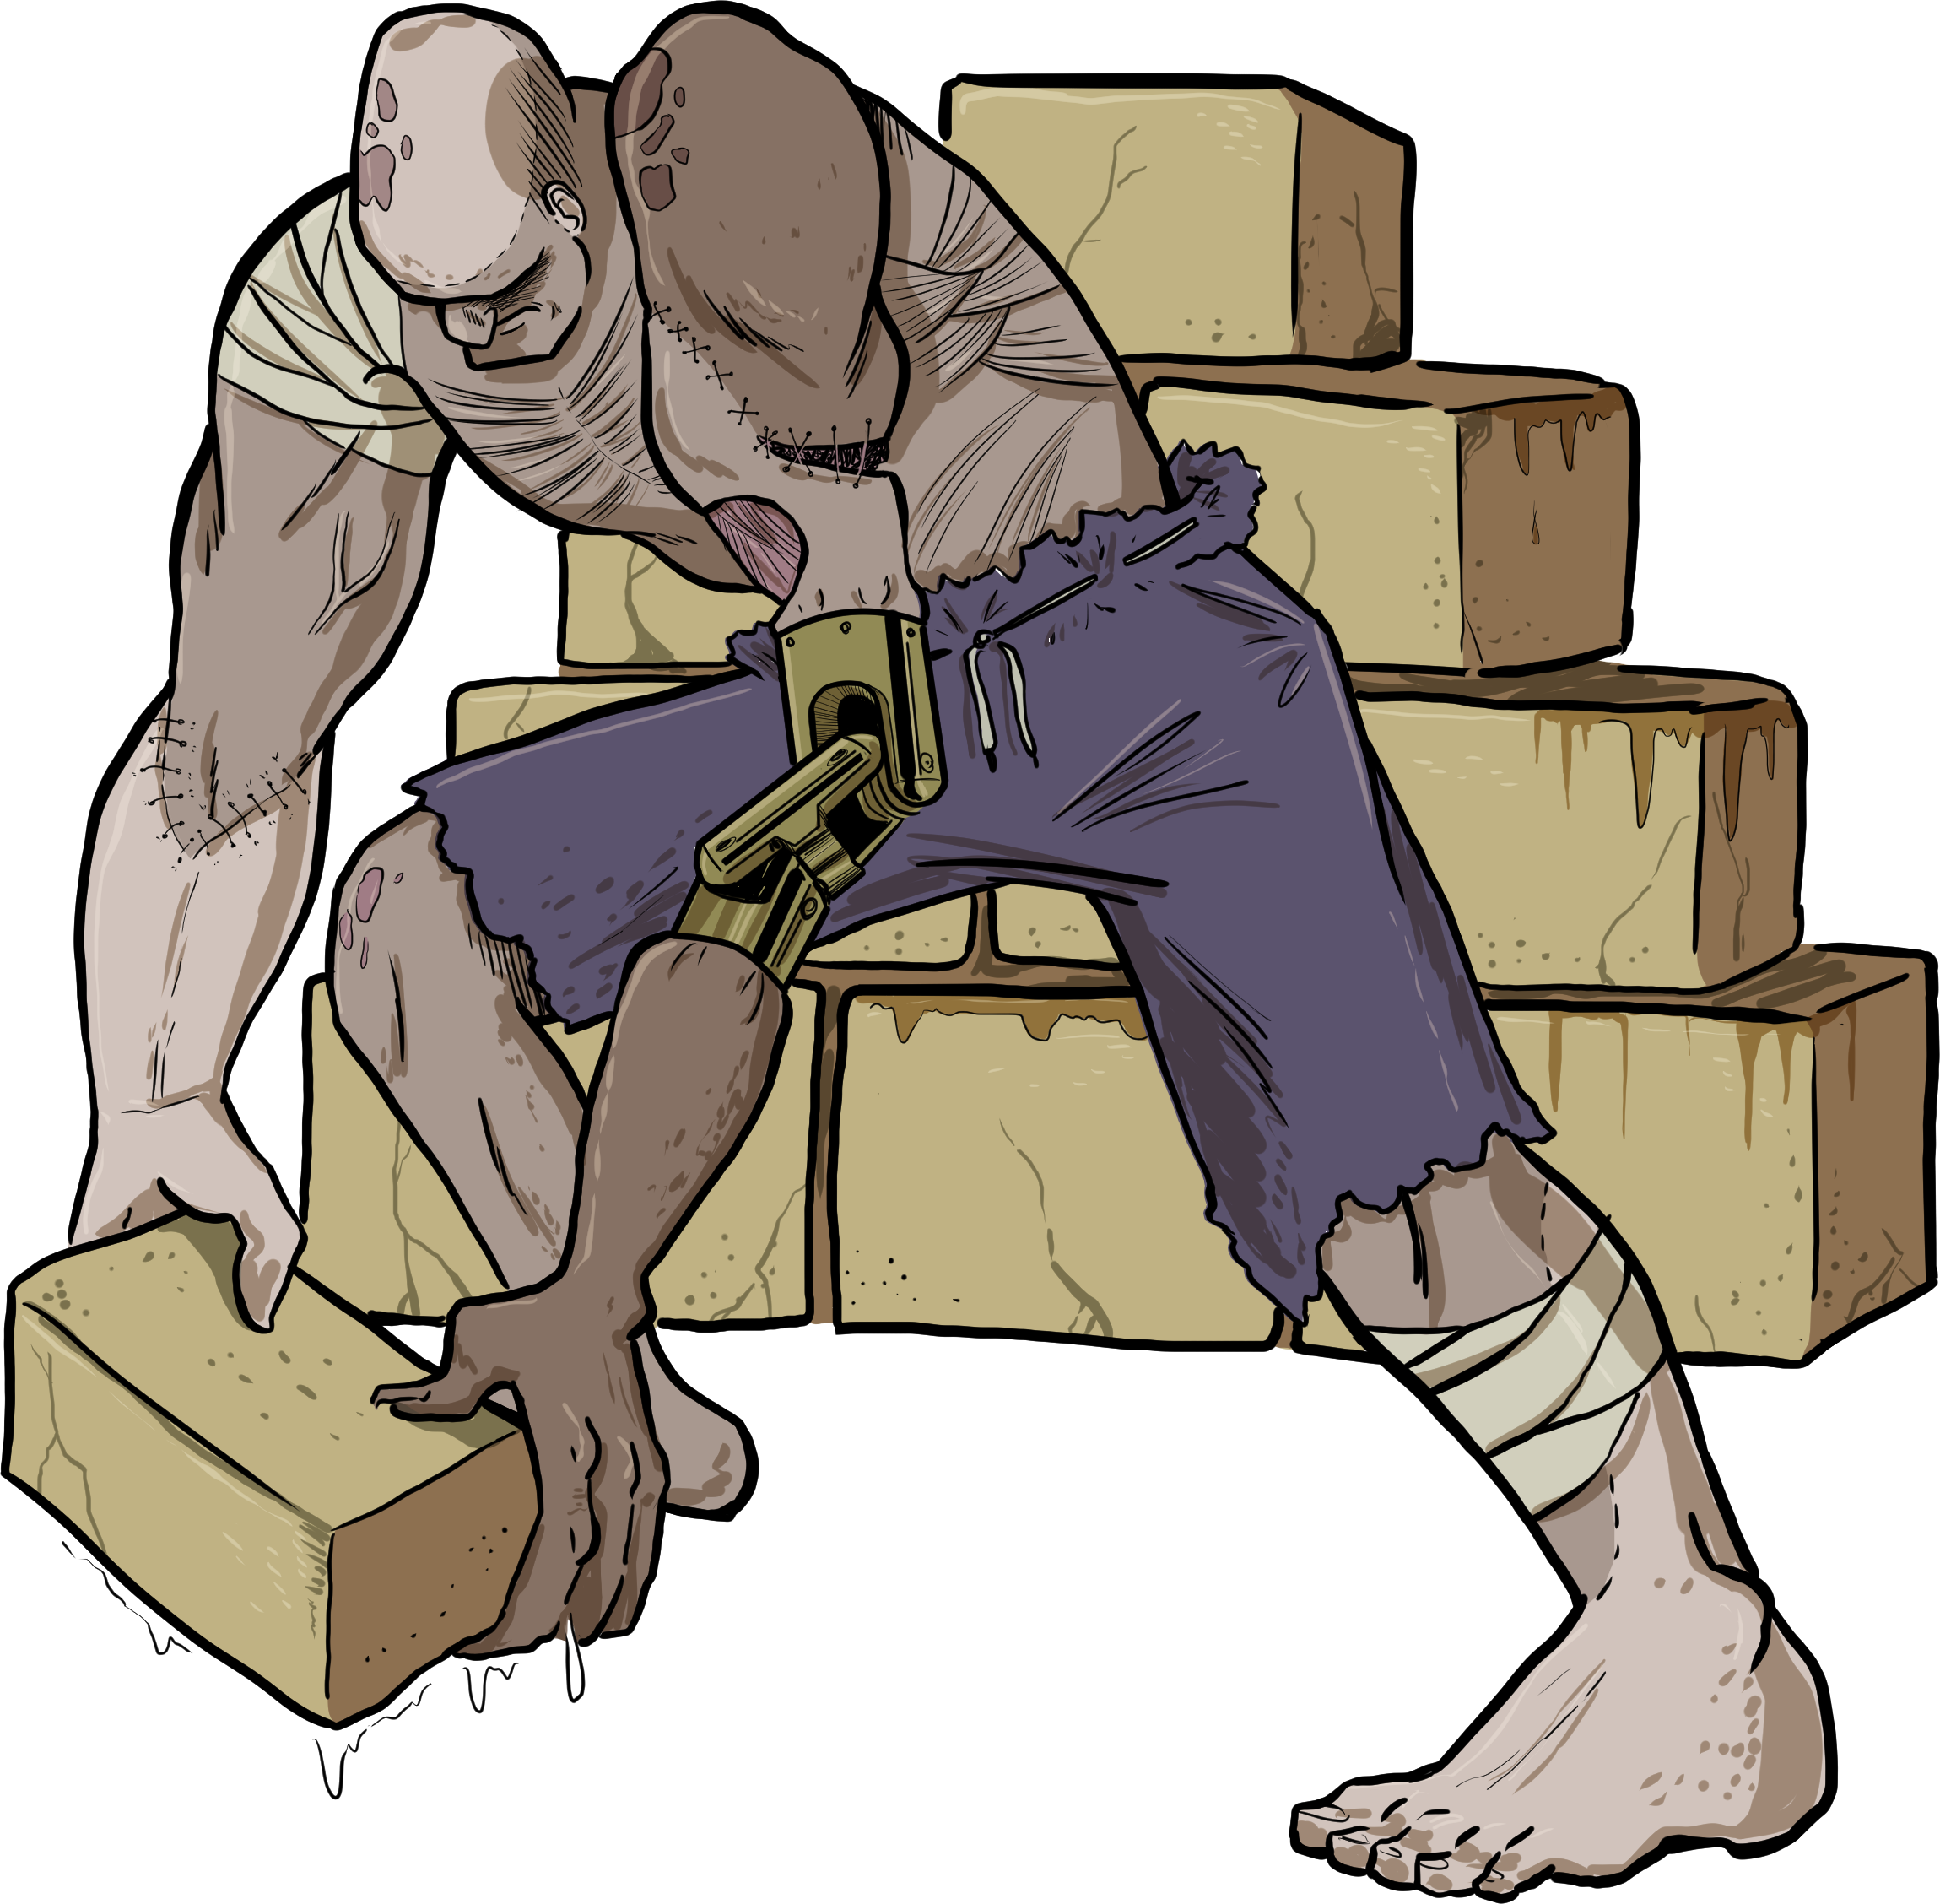
\includegraphics[width=\columnwidth]{Monsters/Golem, Flesh}

\subsubsection{Iron Golem}\index[monsters]{Iron Golem}
\statblock{\textbf{Size:} Large

\textbf{Type:} Construct

\textbf{Habitat:} Any (Rare)

\textbf{Wandering Group:} 1 (Nil)

\textbf{Lair Group:} 1 (Nil)

\textbf{Move:} 80 ft.

\textbf{Armor Class:} 0*

\textbf{Hit Dice:} 20** (90 HP)

\textbf{Attacks:} Hammer Fist (3d10)

\textbf{Special:} Fiery, Immunity (Fire, Gases, 

Mind Effects, Normal Weapons, Poison)

\textbf{Save:} F10

\textbf{Alignment:} None

\textbf{Intelligence:} 4

\textbf{Morale:} 12

\textbf{XP Value:} 5,975}

An iron golem is a humanoid with a red-hot skin of riveted iron plates and a fiery inside. Its two hands are formed into a hammer and tongs, and if given a supply of metal it can make weapons and armor autonomously by opening its chest cavity and using itself as a forge.

\textbf{Fiery:} Anyone hit by an iron golem takes an extra 1d10 fire damage from the heat inside it, and anyone who hits an iron golem with an edged weapon must make a saving throw vs. death ray or take 2d6 fire damage from the fire and molten metal that spurts from the wound.

\subsubsection{Mud Golem}\index[monsters]{Mud Golem}
\statblock{\textbf{Size:} Medium

\textbf{Type:} Construct

\textbf{Habitat:} Any (Rare)

\textbf{Wandering Group:} 1 (Nil)

\textbf{Lair Group:} 1 (Nil)

\textbf{Move:} 30 ft.

\textbf{Armor Class:} 9*

\textbf{Hit Dice:} 8* (36 HP)

\textbf{Attacks:} Hug (2d6)

\textbf{Special:} Immunity (Gases, Mind Effects, 

Normal Weapons, Poison), Smother

\textbf{Save:} F8

\textbf{Alignment:} None

\textbf{Intelligence:} 4

\textbf{Morale:} 12

\textbf{XP Value:} 1,200}

A mud golem is made entirely from mud held together by magical enchantments.

\textbf{Smother:} A mud golem attacks by trying to smother its victim. If one succeeds with a hug attack, it continues to do 2d6 damage per round without needing to hit again.

\subsubsection{Obsidian Golem}\index[monsters]{Obsidian Golem}
\statblock{\textbf{Size:} Large

\textbf{Type:} Construct

\textbf{Habitat:} Any (Rare)

\textbf{Wandering Group:} 1 (Nil)

\textbf{Lair Group:} 1 (Nil)

\textbf{Move:} 40 ft.

\textbf{Armor Class:} 3*

\textbf{Hit Dice:} 6* (27 HP)

\textbf{Attacks:} Weapon (By weapon)

\textbf{Special:} Immunity (Gases, Mind Effects, 

Normal Weapons, Poison)

\textbf{Save:} F3

\textbf{Alignment:} None

\textbf{Intelligence:} 4

\textbf{Morale:} 12

\textbf{XP Value:} 500}

An obsidian golem is a humanoid figure made of sharp shards of obsidian.

Although not truly intelligent, obsidian golems can speak and can be instructed to perform specific actions or say specific phrases in response to other phrases. This ability allows them to be used as messengers or guards for password protected doors.

\subsubsection{Wood Golem}\index[monsters]{Wood Golem}
\statblock{\textbf{Size:} Small

\textbf{Type:} Construct

\textbf{Habitat:} Any (Rare)

\textbf{Wandering Group:} 1 (Nil)

\textbf{Lair Group:} 1 (Nil)

\textbf{Move:} 40 ft.

\textbf{Armor Class:} 7*

\textbf{Hit Dice:} 2+2 (11 HP)

\textbf{Attacks:} Fist (1d8)

\textbf{Special:} Immunity (Gases, Mind Effects, Normal Weapons, Poison), Susceptibility to Fire

\textbf{Save:} F1

\textbf{Alignment:} None

\textbf{Intelligence:} 4

\textbf{Morale:} 12

\textbf{XP Value:} 35}

A wood golem is an animated humanoid figure comprised of tangled branches, twigs, and lumber of various shapes and sizes.

Wood golems move stiffly which gives them a -1 penalty to initiative.

\textbf{Susceptibility to Fire:} Wood golems burn easily giving them a -2 penalty to all saving throws against fire-based attacks and causing them to take +1 point of fire damage per die in the attack.

\subsection{Gorgon}\index[monsters]{Gorgon}
\begin {table}[H]
	\normalsize
	\begin{tabularx}{\columnwidth}{@{}>{\bfseries}lXX@{}}
	\hiderowcolors
	& \textbf{Prime Plane} & \textbf{Home Plane}\\
	Size: & Large & Large\\
	Type: & Extraplanar, & Monster\\
	& Monster\\
	Habitat: & Clear (Very Rare) & Elemental Plane of Earth (Very Rare)\\
	Wandering Group: & 1d2 (Nil) & 1d8 (Nil)\\
	Lair Group: & 1d4 (E) & 3d12 (Nil)\\
	Move: & 40 ft. & 40 ft.\\
	Armor Class: & 2 & 2\\
	Hit Dice: & 8* (36 HP) & 4 (18 HP)\\
	Attacks: & Horn (2d6) & Horn (1d4)\\
	Special: & \multicolumn{2}{c}{Breath Weapon, Charge}\\
	& \multicolumn{2}{c}{Immunity to Petrification}\\
	Save: & F8 & F4\\
	Alignment: & None & None\\
	Intelligence: & 1 & 1\\
	Morale: & 8 & 5\\
	XP Value: & 1,200 & 75\\
	\showrowcolors
  \end {tabularx}
\end {table}

Gorgons are magical creatures that look like bulls with iridescent metal scales. They have a bull-like temperament, normally ignoring creatures it sees but not hesitating to attack anything that looks threatening or gets too close.

\textbf{Breath Weapon:} Gorgons can breathe out a 60 feet long and 10 feet wide cloud of petrifying vapor. All those within the cloud must make a saving throw vs. breath weapon or be turned to stone.

\textbf{Charge:} When a gorgon attacks with their horns, they may do a Charge action.

\subsubsection{Home Plane}
Gorgons originate from the Elemental Plane of Earth. There they are considered herd animals and are bred for their milk or meat.

\textbf{Breath Weapon:} A gorgon's breath weapon is only effective against creatures not made of earth.

\subsection{Gremlin}\index[monsters]{Gremlin}
\statblock{\textbf{Size:} Small

\textbf{Type:} Monster

\textbf{Habitat:} Any (Rare)

\textbf{Wandering Group:} 1d6 (Nil)

\textbf{Lair Group:} 1d6 (Nil)

\textbf{Move:} 40 ft.

\textbf{Armor Class:} 7*

\textbf{Hit Dice:} 1+1** (6 HP)

\textbf{Attacks:} Special

\textbf{Special:} Aura of Chaos, Backfire

\textbf{Save:} E1

\textbf{Alignment:} Chaotic

\textbf{Intelligence:} 9

\textbf{Morale:} 12

\textbf{XP Value:} 22}

Gremlins are green humanoids that bear a striking resemblance to goblins, although they are rarely found together. They are mischievous pranksters who find other's failures hilarious, especially when cause by their aura of chaos.

\textbf{Aura of Chaos:} Gremlins radiate an aura of chaos within 20 feet. Within that area, anyone who takes any kind of physical action (e.g. using a skill, or casting a spell, or making an attack) must make a saving throw vs. spells or have the action fail.

Machinery within the aura's radius is also negatively affected. Screws become loose, gears get stuck, or any other mishaps that the Game Master decides on.

\textbf{Backfire:} Anyone who tries to attack a gremlin and fails (whether due to the gremlin’s chaos aura or not) must re-roll their attack against themselves. Similarly, anyone trying to cast a spell on a gremlin who fails is affected by their own spell.

\subsubsection{As a Class}\index[classes]{Gremlin}
Gremlins can be used as a class using the following statistics:

\textbf{Aura of Chaos:} The radius of the aura is listed on \fullref{tab:Gremlin Special Abilities Progression}. Victims of the aura receive a modifier to their saving throw when trying to avoid the effects. This modifier is listed on the same table.

At later levels, gremlins can target creatures within their aura with the following effects:

\textbf{Backfire:} Victims receive a modifier to their hit roll when attacking themselves. This modifier is listed on \fullref{tab:Gremlin Special Abilities Progression}.

\textbf{Hide in Crannies:} A gremlin is able to effectively hide in small narrow spaces. The percentage chance of success is listed in \fullref{tab:Gremlin Special Abilities Progression}. Success indicates that the gremlin is completely hidden and will remain that way until they move.

The Game Master should roll the dice when the gremlin is hiding, so that the gremlin’s player does not know whether or not their character has been spotted. If someone is watching the gremlin before they start to hide, they will still be able to see the gremlin regardless of the success or otherwise of this ability.

\textbf{Misuse Magic Item:} Gremlins have a difficult time properly using magic items. When a gremlin attempts to use a magic item, there is a 10\% chance per level (min 10\%, max of 90\%) that it will malfunction or become entirely useless. A useless magic item begins functioning normally again after 2d4 days away from the gremlin. Each time a gremlin gains a level, there is another chance of failure. The Game Master should make all of these rolls and should also come up with creative outcomes when a malfunction occurs.

\textbf{Resistance to Mind Effects:} Gremlins are very resistant to mind effects. They receive a bonus when saving against these types of effects. The bonus depends on the gremlin's level which is indicated on \fullref{tab:Gremlin Special Abilities Progression}.

\textbf{Slow Fall:} If a gremlin falls, they do not take damage from the first 10 feet of the fall (see \fullref{sec:Environmental Damage}). 

Starting at \nth{1} level, gremlins can fall up to 20 feet without taking damage.

\textbf{Leg Lasso:} Starting at \nth{3} level, twice per day, a gremlin can point at a target's legs and summon a shimmering green lasso tightly around them for 2d4 rounds. The target must be within the gremlin's Aura of Chaos radius to be affected by this ability.

The victim may save vs. spells to avoid the lasso. Large creatures gain a +2 bonus to this save. If the save fails, the victim cannot run or walk and can only hop at 1/\nth{5} their normal speed.

If the victim was running while lassoed they must make a \iref[sec:Dexterity]{Dexterity} check to avoid falling. If the victim fails they fall flat on their face and suffer 1d3 points of damage.

\textbf{Uncontrollable Hideous Laughter:} Starting at \nth{6} level, twice per day, a gremlin can cause a target to laugh uncontrollable by spontaneously jumping out towards them and making an obscene pose or a ridiculous face. The effects of this ability are identical to the spell Uncontrollable Hideous Laughter, but the victim suffers a -2 penalty to their saving throw and the radius is equal to the gremlin's Aura of Chaos radius. A new saving throw is allowed each around to negate the effect.

\textbf{Confusion:} Once per day at \nth{9} level and higher, a gremlin can cause a target to become confused as the Confusion spell.

\statblock{\textbf{Ability Requirements:} Dexterity 6

\textbf{Prime Requisite:} Dexterity

\textbf{Ability Modifiers:} None

\textbf{Weapons:} Dagger or sling

\textbf{Armor:} None

\textbf{Natural AC:} 7

\textbf{Special Abilities:} Aura of Chaos, Backfire, Jump, Misuse Magic Item, Resistance to Mind Effects, Slow Fall, Leg Lasso, Hideous Laughter, Confusion

\textbf{Required Skills:} Jumping (plus an additional 2 points by \nth{5} level)

\textbf{Magic Item Use:} Fighter (Chance of Misuse)}

\begin {table}[H]
  \caption{Gremlin Progression}
  \begin{tabularx}{\columnwidth}{>{\bfseries}YYY}
	\thead{Level} & \thead{Experience} & \thead{Hit Dice}\\
	-1 & -3,000 & 1d8\\
	0 & 0 & -\\
	1 & 3,000 & 1d8+1\\
	2 & 9,000 & 2d8+1\\
	3 & 21,000 & 2d8+2\\
	4 & 45,000 & 3d8+2\\
	5 & 95,000 & 3d8+3\\
	6 & 190,000 & 4d8+3\\
	7 & 380,000 & 4d8+4\\
	8 & 680,000 & 5d8+4\\
	9+ & +300,000 & +2 HP
  \end {tabularx}
\end {table}

\begin {table}[H]
  \caption{Gremlin Special Abilities Progression}\label{tab:Gremlin Special Abilities Progression}
  \begin{tabularx}{\columnwidth}{>{\bfseries}ccccYY}
	\thead{} & \multicolumn{2}{c}{\thead{Aura of Chaos}} & \thead{} & \thead{} & \thead{}\\
	\thead{Level} & \thead{Radius} & \thead{Save} & \thead{Backfire} & \thead{Hide in Crannies} & \thead{Resistance to Mind Effects}\\
	-1 & 5' & +3 & -4 & 25\% & +1\\
	0 & 8' & +2 & -3 & 35\% & +1\\
	1 & 10' & +2 & -3 & 40\% & +2\\
	2 & 12' & +1 & -2 & 45\% & +2\\
	3 & 14' & +1 & -2 & 50\% & +2\\
	4 & 15' & +1 & -2 & 55\% & +3\\
	5 & 16' & 0 & -1 & 60\% & +3\\
	6 & 17' & 0 & -1 & 65\% & +3\\
	7 & 18' & 0 & -1 & 70\% & +3\\
	8 & 19' & -1 & -1 & 75\% & +3\\
	9+ & 20' & -1 & 0 & 80\% & +4
  \end {tabularx}
\end {table}

\subsection{Gray Ooze}\index[monsters]{Gray Ooze}
\monsterimage{Monsters/Gray Ooze}{\statblock{\textbf{Size:} Medium

\textbf{Type:} Ooze

\textbf{Habitat:} Underground (Common)

\textbf{Wandering Group:} 1d4 (Nil)

\textbf{Lair Group:} 1d4 (Nil)

\textbf{Move:} 3 ft.

\textbf{Armor Class:} 8*

\textbf{Hit Dice:} 3* (14 HP)

\textbf{Attacks:} Touch (Special)

\textbf{Special:} Engulf, Immunity (Cold, Fire)

\textbf{Save:} F2

\textbf{Alignment:} None

\textbf{Intelligence:} 0

\textbf{Morale:} 12

\textbf{XP Value:} 50}}

A gray ooze looks like a blob or boulder of wet stone until it moves.

Gray oozes will attack anything that comes close to it.

\textbf{Engulf:} If a gray ooze hits an opponent, it starts to dissolve their clothing and armor. Non-magical clothing or armor can be dissolved in a single round, but a gray ooze cannot eat through magical clothing or armor. If it finds itself engulfing a victim that it can’t digest, it will release the victim and try to engulf a different one.

Once a gray ooze has dissolved its victims armor or clothing, its acid will do 2d8 points of damage per round to the victim.

\subsection{Griffon}\index[monsters]{Griffon}\label{monster:Griffon}
\statblock{\textbf{Size:} Large

\textbf{Type:} Monster

\textbf{Habitat:} Mountains (Rare)

\textbf{Wandering Group:} 1 (Nil)

\textbf{Lair Group:} 2d8 (E)

\textbf{Move:} 40 ft., 120 ft. (Fly)

\textbf{Armor Class:} 5

\textbf{Hit Dice:} 7 (32 HP)

\textbf{Attacks:} 2x Claw (1d4) \& Bite (2d8)

\textbf{Special:} None

\textbf{Save:} F4

\textbf{Alignment:} None

\textbf{Intelligence:} 2

\textbf{Morale:} 8

\textbf{XP Value:} 450}

A griffon is a creature with the head, wings and front claws of a giant eagle, and the body, back legs and tail of a lion.

Griffons are predators and will eat almost anything. However, their favorite food is horse. A griffon—even a tamed one—within 120 feet of a horse must make a morale check. If it fails, it will attack the horse and try to eat it.

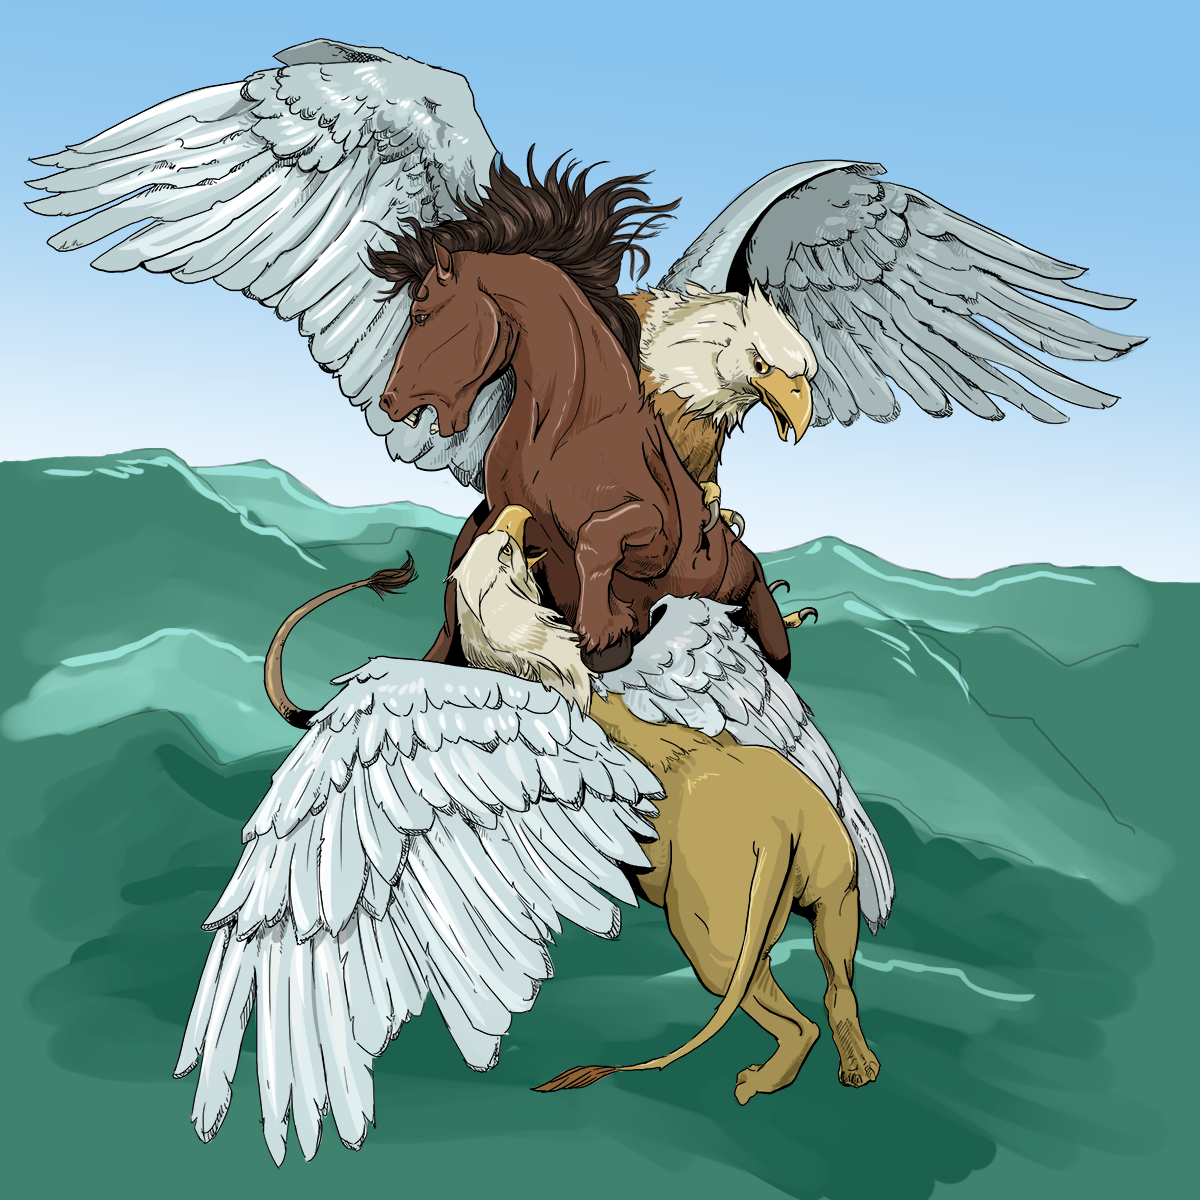
\includegraphics[width=\columnwidth]{Monsters/Griffon}

\subsection{Hag, Night}\index[monsters]{Night Hag}
\statblock{\textbf{Size:} Medium

\textbf{Type:} Humanoid

\textbf{Habitat:} Woods (Very Rare)

\textbf{Wandering Group:} 1 (Nil)

\textbf{Lair Group:} 1 (C)

\textbf{Move:} 50 ft., 20 ft. (Swim)

\textbf{Armor Class:} 4

\textbf{Hit Dice:} 15***** (68 HP)

\textbf{Attacks:} 2x Claw (1d4) or Spell

\textbf{Special:} Cleric Spells, Control Undead, 

Immunity to Undead Special Abilities, Poison

\textbf{Save:} C15

\textbf{Alignment:} Chaotic

\textbf{Intelligence:} 12

\textbf{Morale:} 10

\textbf{XP Value:} 6,9000}

Night hags are cannibalistic humanoids who appear to be ugly female humans with warty blue-black skin and black hair.

They live in isolation in small cottages deep in forests, where they surround themselves with undead minions.

Night hags are incredibly anti-social but will often make a pretense at friendliness in order to trap potential victims.

\textbf{Cleric Spells:} A night hag can cast spells as a \nth{15} level cleric.

\textbf{Control Undead:} A night hag can control undead as if a 30 hit dice Undead Liege.

\textbf{Poison:} The claws of a night hag are extremely poisonous, and anyone struck by one must make a saving throw vs. poison with a -4 penalty or die.

\subsection{Hag, Sea}\index[monsters]{Sea Hag}
\statblock{\textbf{Size:} Medium

\textbf{Type:} Humanoid

\textbf{Habitat:} Ocean (Very Rare)

\textbf{Wandering Group:} 1 (Nil)

\textbf{Lair Group:} 1 (G+M)

\textbf{Move:} 40 ft., 50 ft. (Swim)

\textbf{Armor Class:} 4*

\textbf{Hit Dice:} 8**** (36 HP)

\textbf{Attacks:} Dagger (1d4) \& Touch (Special)

\textbf{Special:} Despair, Immunity (Non-Silver 

Normal Weapons), Undead Abilities, Waning Touch

\textbf{Save:} F8

\textbf{Alignment:} Chaotic

\textbf{Intelligence:} 12

\textbf{Morale:} 10

\textbf{XP Value:} 2,850}

Sea hags are foul humanoids who appear to be incredibly ugly female humans with yellow-green skin and green hair.

Sea hags live underwater in coastal area, although they can come onto the land for up to three hours at a time.

\textbf{Control Undead:} A sea hag can control undead as if a 16 hit dice Undead Liege.

\textbf{Despair:} Sea hags are so disgusting and filth encrusted that anyone who sees one or who approaches within 10 feet of one must make a saving throw vs. spells with a -6 penalty to avoid fleeing in fear for 1d20+5 rounds.

\textbf{Waning Touch:} The touch of a sea hag acts as both an \ilink{spell:Energy Drain}{Energy Drain} of one level and a \ilink{spell:Cause Disease}{Cause Disease}. There is no saving throw against either effect.

\subsection{Halfling}\index[monsters]{Halfling}
\statblock{\textbf{Size:} Small

\textbf{Type:} Demi-Human

\textbf{Habitat:} Clear, Hills (Common)

\textbf{Wandering Group:} 3d6 (P+S)

\textbf{Lair Group:} 5d8 (B)

\textbf{Move:} 30 ft.

\textbf{Armor Class:} 7

\textbf{Hit Dice:} 1-1 (4 HP)

\textbf{Attacks:} Weapon (By weapon)

\textbf{Special:} As \nth{1} level Halfling

\textbf{Save:} H1

\textbf{Alignment:} Lawful

\textbf{Intelligence:} 11

\textbf{Morale:} 8

\textbf{XP Value:} 5}

Halflings are a demi-human race, much shorter and lighter than humans, standing only 3 feet tall. They are of a proportionally similar build to humans, with the exception of their feet—which are large and covered in hair. The soles of halflings feet are tough and resilient, and halflings often travel bare-footed.

Halflings’ skin tone has a similar range to that of humans, as does their hair color. Halflings do not grow beards or mustaches, but the sideburns of adult males tend to be longer than those of humans.

Halflings are very gregarious and can be commonly found living amongst humans and other demi-humans. If left to themselves, they form small villages in grasslands and hills where they excel at farming.

Halfling food production and the halfling love of cookery and brewing make them very popular amongst the other races.

\subsection{Harpy}\index[monsters]{Harpy}
\statblock{\textbf{Size:} Medium

\textbf{Type:} Monster

\textbf{Habitat:} Hills, Mountains (Rare)

\textbf{Wandering Group:} 1d6 (Nil)

\textbf{Lair Group:} 2d4 (C)

\textbf{Move:} 20 ft., 50 ft. (Fly+Special)

\textbf{Armor Class:} 7

\textbf{Hit Dice:} 3*

\textbf{Attacks:} 2x Claw (1d4) or Weapon (By weapon) 

or Bite (1d6)

\textbf{Special:} Captivating Song, Disease

\textbf{Save:} F6

\textbf{Alignment:} Chaotic

\textbf{Intelligence:} 7

\textbf{Morale:} 7

\textbf{XP Value:} 50}

Harpies look like eagles with the heads (and breasts in the case of female harpies) of beautiful elves.

Harpies usually nest near mountain paths, and try to pick off lone travelers. If they encounter a large or heavily armed group, they will usually hide or try to use their charm ability in self defense.

\textbf{Captivating Song:} The singing of a harpy of either gender acts as a \iref[spell:Charm Person]{Charm Person} spell, and harpies use this charm to lure travelers. into ambushes. Any character that makes their saving throw against the singing of a harpy is immune to that particular harpy’s song for the rest of the encounter.

\textbf{Disease:} Harpy bites have a 5\% chance of transmitting a disease. If this is the case, the victim is affected as if by a Cause Disease spell (complete with saving throw).

\textbf{Fly:} Harpies can fly for a number of hours per day equal to their \iref[sec:Constitution]{Constitution} score to a maximum of 14.

\subsubsection{Spellcasting}
Harpies can be shamans (to \nth{6} level) or sorcerers (to \nth{4} level).

\subsubsection{As a Class}\index[classes]{Harpy}
Harpies can be used as a class using the following statistics:

\textbf{Captivating Song:} Victims of an immature harpy's song gain a bonus to their saving throw equal to the harpy's immaturity level.

\textbf{Captivating Touch:} Once per day at \nth{4} level and higher, a harpy may charm a person by touching them. The effects of this ability are identical to the harpy's captivating song ability except the victim suffers a -2 penalty to their saving throw.

At \nth{6} level and higher, this ability can also be used on monsters. 

At \nth{7} level and higher, harpies can use this ability on monsters up to 3 times a day.

\textbf{Fly:} Immature harpies can only fly a number of hours per day equal to 1/3 of their \iref[sec:Constitution]{Constitution} score at level -2 and 1/2 at level -1.

\textbf{Infectious Bite:} Harpy PCs do not transmit a disease when they bite a victim as they are more well-kept compared to regular harpies.

\statblock{\textbf{Ability Requirements:} None

\textbf{Prime Requisite:} Strength

\textbf{Ability Modifiers:} None

\textbf{Weapons:} Any melee

\textbf{Armor:} None

\textbf{Natural AC:} 7

\textbf{Special Abilities:} Captivating Song, Captivating Touch, Fly, Infectious Bite

\textbf{Magic Item Use:} Fighter}

\begin {table}[H]
  \caption{Harpy Progression}
  \begin{tabularx}{\columnwidth}{>{\bfseries}YYY}
	\thead{Level} & \thead{Experience} & \thead{Hit Dice}\\
	-2 & -6,000 & 1d8\\
	-1 & -3,000 & 2d8\\
	0 & 0 & 3d8\\
	1 & 6,000 & 4d8\\
	2 & 18,000 & -\\
	3 & 42,000 & 5d8\\
	4 & 90,000 & 6d8\\
	5 & 180,000 & 7d8\\
	6 & 360,000 & -\\
	7 & 660,000 & 8d8\\
	8 & 960,000 & 9d8\\
	9+ & +300,000 & +2 HP
  \end {tabularx}
\end {table}

\subsection{Haunt}
A haunt is an undead spirit of a creature that is unable to rest. Haunts are usually found near the area where their mortal body died.

A haunt can only be harmed by +2 weapons or better.

\textbf{Immunity to Spells:} A haunt is immune to all spells except those that specifically target evil or undead.

\textbf{Planar Travel:} Haunts can move to the \iref[sec:Ethereal Plane]{Ethereal Plane} three times per day, and can leave it at any time.

They can also secrete a web of ectoplasm tendrils around themselves in a 10-foot radius that takes three rounds to form (while taking other actions). Anyone who enters the radius once formed must save vs. spells or be transported to the \iref[sec:Ethereal Plane]{Ethereal Plane}.

\textbf{Turn Resistance:} A haunt can make a saving throw vs. spells to avoid a ‘d’ or ‘D’ result when being turned.

\subsubsection{Banshee}\index[monsters]{Banshee}
\statblock{\textbf{Size:} Medium

\textbf{Type:} Undead

\textbf{Habitat:} Any (Very Rare)

\textbf{Wandering Group:} 1 (Nil)

\textbf{Lair Group:} 1 (E, N, O)

\textbf{Move:} 20 ft.

\textbf{Armor Class:} -3*

\textbf{Hit Dice:} 13**** (59 HP)

\textbf{Attacks:} None

\textbf{Special:} Immunity (Mind Effects, Poison, Spells), 

Paralyzing Gaze, Planar Travel, Senescent, Turn Resistance, Wail

\textbf{Save:} F13

\textbf{Alignment:} Chaotic

\textbf{Intelligence:} 12

\textbf{Morale:} 9

\textbf{XP Value:} 5,150}

A banshee is an undead spirit that protects an outdoor location that it had a connection to in life from all intruders.

\textbf{Paralyzing Gaze:} The gaze of a banshee paralyzes its target for 2d4 rounds unless the target can make a saving throw vs. spells.

\textbf{Senescent:} The touch of a banshee ages its target by 1d4x10 years (no save).

\textbf{Wail:} Three times per day, a banshee can wail, causing all in 60 feet to save vs. death or die. A banshee will often wail while out of range as a warning to potential intruders.

\subsubsection{Ghost}\index[monsters]{Ghost}
\statblock{\textbf{Size:} Medium

\textbf{Type:} Undead

\textbf{Habitat:} Any (Very Rare)

\textbf{Wandering Group:} 1 (Nil)

\textbf{Lair Group:} 1 (E, N, O)

\textbf{Move:} 30 ft.

\textbf{Armor Class:} -2*

\textbf{Hit Dice:} 14**** (63 HP)

\textbf{Attacks:} None

\textbf{Special:} Immunity (Mind Effects, Poison), Magic Jar, 

Paralyzing Gaze, Planar Travel, Senescent, Turn Resistance

\textbf{Save:} F13

\textbf{Alignment:} Any

\textbf{Intelligence:} 13

\textbf{Morale:} 11

\textbf{XP Value:} 5,500}

A ghost is an undead spirit that tries to fulfill a task it left unfinished in life.

\textbf{Magic Jar:} A ghost can use the Magic Jar spell once per ten minutes, and will often use this to possess a target and use the target’s body to fulfill its task, either with or without permission of the target.

\textbf{Paralyzing Gaze:} The gaze of a ghost paralyzes its target for 2d4 rounds unless the target can make a saving throw vs. spells.

\textbf{Senescent:} The touch of a ghost ages its target by 1d4x10 years (no save).

\subsubsection{Poltergeist}\index[monsters]{Poltergeist}
\statblock{\textbf{Size:} Medium

\textbf{Type:} Undead

\textbf{Habitat:} Any (Very Rare)

\textbf{Wandering Group:} 1 (Nil)

\textbf{Lair Group:} 1 (E, N, O)

\textbf{Move:} 20 ft.

\textbf{Armor Class:} -1*

\textbf{Hit Dice:} 12**** (54 HP)

\textbf{Attacks:} 2x Throw (1d4)

\textbf{Special:} Immunity (Mind Effects, Poison), Natural Invisibility, 

Planar Travel, Senescent, Throw Objects, Turn Resistance

\textbf{Save:} F11

\textbf{Alignment:} Chaotic

\textbf{Intelligence:} 13

\textbf{Morale:} 11

\textbf{XP Value:} 4,750}

A poltergeist is the undead spirit of a dead child.

A poltergeist is normally more mischievous than aggressive, although it will react angrily to any insult or any attempt to get rid of it and try to kill the offender.

\textbf{Senescent:} Any target hit by an object thrown by a poltergeist will be aged by 10 years unless they can make a saving throw vs. spells.

\textbf{Throw Objects:} A poltergeist can throw small objects around. When not angered, a poltergeist will usually deliberately miss their targets.

\subsubsection{Haunt, Spook}\index[monsters]{Spook}
\statblock{\textbf{Size:} Medium

\textbf{Type:} Undead

\textbf{Habitat:} Any (Very Rare)

\textbf{Wandering Group:} 1-2 (Nil)

\textbf{Lair Group:} 1-2 (E, N, O)

\textbf{Move:} Nil

\textbf{Armor Class:} Not applicable

\textbf{Hit Dice:} Not applicable

\textbf{Attacks:} None

\textbf{Special:} Despair, Immunity (Mind Effects, Poison)

\textbf{Save:} F9

\textbf{Alignment:} Any

\textbf{Intelligence:} 10

\textbf{Morale:} Not applicable

\textbf{XP Value:} 100 (see below)}

A spook is a ghostly spirit of a creature that is unable to rest due to an unfinished task and is bound to a particular location. The location tends to be an area where the creature died.

Spooks cannot be killed, they must be laid to rest by conditions decided by the Game Master. Experience points are only awarded to characters if they helped the spook fulfill these conditions.

\textbf{Despair:} Spooks cannot attack or inflict any damage. Characters who encounter the spook must make a save vs. spells or run in fear, never to willingly return to the location again.

\subsection{Hellhound}\index[monsters]{Hellhound}
\statblock{\textbf{Size:} Medium

\textbf{Type:} Monster

\textbf{Habitat:} Mountains, Underground (Rare)

\textbf{Wandering Group:} 2d4 (Nil)

\textbf{Lair Group:} 2d4 (C)

\textbf{Move:} 40 ft.

\textbf{Armor Class:} 4*

\textbf{Hit Dice:} 3** (14 HP)

\textbf{Attacks:} Bite (1d6) or Special

\textbf{Special:} Breath Weapon, Detect Invisibility, Immunity to Non-Magical Fire

\textbf{Save:} F3

\textbf{Alignment:} Chaotic

\textbf{Intelligence:} 12

\textbf{Morale:} 9

\textbf{XP Value:} 65}

Hellhounds are wolf-like creatures with reddish-brown fur and glowing red eyes. They tend to live in or near volcanoes or underground.

Despite their appearance as little more than dogs, hellhounds are sapient, and are as intelligent as humans.

\textbf{Breath Weapon:} A hellhound may breathe fire at a single opponent within 10 feet. This fire breath does 3d6 damage, although the target may make a saving throw vs. dragon breath to take half damage.

\textbf{Detect Invisibility:} Hellhounds have acute senses that allow them to constantly Detect Invisible.

\subsection{Herd Animal}\index[monsters]{Herd Animal}
\statblock{\textbf{Size:} Medium-Large

\textbf{Type:} Animal

\textbf{Habitat:} Clear, Woods (Common)

\textbf{Wandering Group:} 1 (Nil)

\textbf{Lair Group:} 3d10 (Nil)

\textbf{Move:} 80 ft.

\textbf{Armor Class:} 7

\textbf{Hit Dice:} 2 (9 HP)

\textbf{Attacks:} Butt (1d4+1)

\textbf{Special:} None

\textbf{Save:} F1

\textbf{Alignment:} None

\textbf{Intelligence:} 2

\textbf{Morale:} 5

\textbf{XP Value:} 20}

Herd Animals, ranging from sheep and goats to elks and bison, exist in most parts of the world. They are normally found in extended family groups and small herds, but occasionally a lone male will be found wandering on its own.

Herd animals are not normally aggressive and will usually run from any perceived danger, although some of the larger types may be provoked into circling defensively and protecting their young against the attacks of potential predators.

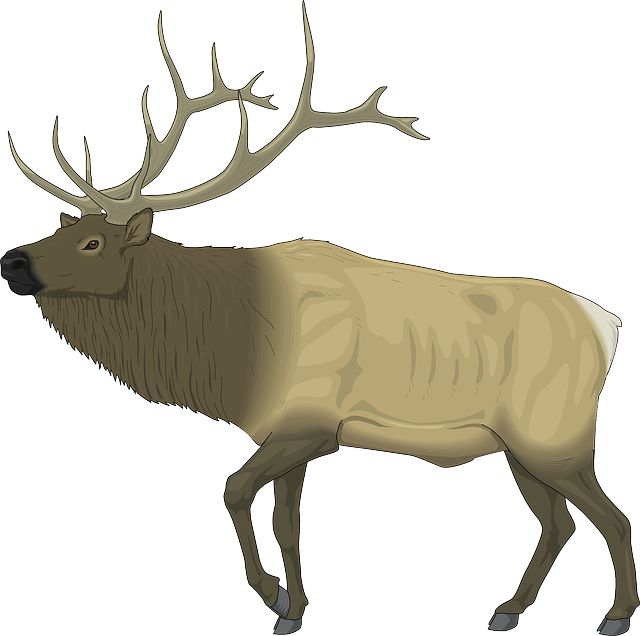
\includegraphics[width=\columnwidth]{Monsters/Animals/Herd Animal}

\subsection{Hippogriff}\index[monsters]{Hippogriff}\label{monster:Hippogriff}
\statblock{\textbf{Size:} Large

\textbf{Type:} Monster

\textbf{Habitat:} Mountains (Rare)

\textbf{Wandering Group:} 0 (Nil)

\textbf{Lair Group:} 2d8 (Nil)

\textbf{Move:} 60 ft., 120 ft. (Fly)

\textbf{Armor Class:} 5

\textbf{Hit Dice:} 3+1 (15 HP)

\textbf{Attacks:} 2x Claw (1d6) \& Bite (1d10)

\textbf{Special:} None

\textbf{Save:} F2

\textbf{Alignment:} None

\textbf{Intelligence:} 3

\textbf{Morale:} 8

\textbf{XP Value:} 50}

A hippogriff is a creature with the head, wings and front claws of a giant eagle, and the body, back legs and tail of a horse.

Griffons are predators and scavengers that normally take only small live prey or chase other creatures off to steal their kills. However, hippogriffs have a fierce hatred of pegasi and will attack them on sight to drive them away. A hippogriff—even a tamed one—within 120 feet of a pegasus must make a morale check. If it fails, it will attack the pegasus and try to kill it or drive it off.

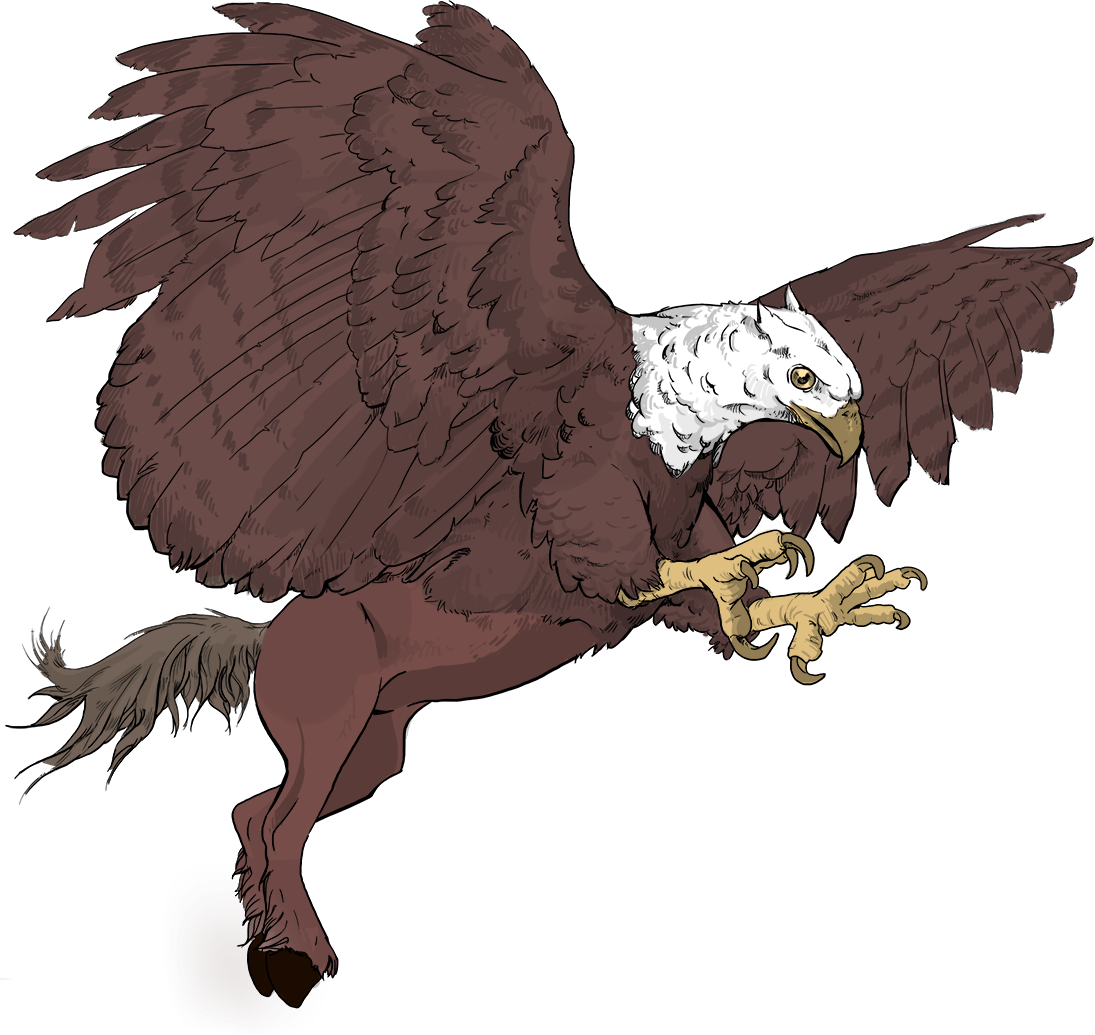
\includegraphics[width=\columnwidth]{Monsters/Hippogriff}

\subsection{Hobgoblin}\index[monsters]{Hobgoblin}
\monsterimage{Monsters/Hobgoblin}{\statblock{\textbf{Size:} Medium

\textbf{Type:} Humanoid

\textbf{Habitat:} Hills, Mountains,\\ 
Underground, Woods (Common)

\textbf{Wandering Group:} 1d6 (Q)

\textbf{Lair Group:} 4d6 (D)

\textbf{Move:} 30 ft.

\textbf{Armor Class:} 6

\textbf{Hit Dice:} 1+1 (6 HP)

\textbf{Attacks:} Weapon (By weapon)

\textbf{Special:} Infravision

\textbf{Save:} F1

\textbf{Alignment:} Chaotic

\textbf{Intelligence:} 10

\textbf{Morale:} 8

\textbf{XP Value:} 15} }

Hobgoblins are larger and stronger cousins of goblins. They look like goblins, but are taller and are more muscular. They have red eyes that glow softly when there is no light.

Hobgoblins do not have their own spellcasters, and this often puts them in a precarious relationship with goblin tribes, as the hobgoblins are naturally more powerful than most of the goblins but cannot dominate them completely because they both fear and need the goblin spellcasters.

\subsubsection{As a Class}\index[classes]{Hobgoblin}
Hobgoblins can be used as a class using the following statistics:

\statblock{\textbf{Ability Requirements:} None

\textbf{Prime Requisite:} Strength, Dexterity, Intelligence, or Wisdom

\textbf{Ability Modifiers:} Strength +1, Dexterity -1

\textbf{Weapons:} Any

\textbf{Armor:} Any

\textbf{Natural AC:} 8

\textbf{Special Abilities:} None

\textbf{Magic Item Use:} Fighter}

\begin {table}[H]
  \caption{Hobgoblin Progression}
  \begin{tabularx}{\columnwidth}{>{\bfseries}YYY}
	\thead{Level} & \thead{Experience} & \thead{Hit Dice}\\
	0 & 0 & 1d8+1\\
	1 & 1,200 & 2d8+2\\
	2 & 2,400 & 3d8+3\\
	3 & 4,800 & -\\
	4 & 9,600 & 4d8+4\\
	5 & 19,000 & 5d8+5\\
	6 & 38,000 & 6d8+5\\
	7 & 76,000 & -\\
	8 & 150,000 & 7d8+5\\
	9 & 300,000 & 7d8+7\\
	10+ & +240,000 & +2 HP
  \end {tabularx}
\end {table}

\subsection{Horse, Draft}\index[monsters]{Draft Horse}
\statblock{\textbf{Size:} Large

\textbf{Type:} Animal

\textbf{Habitat:} Clear (Common)

\textbf{Wandering Group:} 0 (Nil)

\textbf{Lair Group:} 0 (Nil)

\textbf{Move:} 30 ft.

\textbf{Armor Class:} 7

\textbf{Hit Dice:} 3 (14 HP)

\textbf{Attacks:} Bite (1d3)

\textbf{Special:} None

\textbf{Save:} F2

\textbf{Alignment:} None

\textbf{Intelligence:} 2

\textbf{Morale:} 6

\textbf{XP Value:} 35}

Draft horses are bred for strength and stamina rather than speed. They are normally used to pull carts and wagons.

Draft horses are a totally domesticated species, and do not occur in the wild.

\subsection{Horse, Pony}\index[monsters]{Pony}
\statblock{\textbf{Size:} Medium

\textbf{Type:} Animal

\textbf{Habitat:} Clear (Common)

\textbf{Wandering Group:} 0 (Nil)

\textbf{Lair Group:} 5d10 (Nil)

\textbf{Move:} 70 ft.

\textbf{Armor Class:} 7

\textbf{Hit Dice:} 2 (9 HP)

\textbf{Attacks:} 2x Kick (1d4)

\textbf{Special:} None

\textbf{Save:} F1

\textbf{Alignment:} None

\textbf{Intelligence:} 7

\textbf{Morale:} 6

\textbf{XP Value:} 20}

Ponies are mainly domesticated but also occur in the wild.

Because of their small size, ponies are popular mounts for gnomes, halflings and dwarves.

\subsection{Horse, Riding}\index[monsters]{Riding Horse}
\statblock{\textbf{Size:} Large

\textbf{Type:} Animal

\textbf{Habitat:} Clear, Settled (Common)

\textbf{Wandering Group:} 0 (Nil)

\textbf{Lair Group:} 10d10 (Nil)

\textbf{Move:} 80 ft.

\textbf{Armor Class:} 7

\textbf{Hit Dice:} 2 (9 HP)

\textbf{Attacks:} 2x Kick (1d4)

\textbf{Special:} None

\textbf{Save:} F1

\textbf{Alignment:} None

\textbf{Intelligence:} 2

\textbf{Morale:} 7

\textbf{XP Value:} 20}

Riding horses are domesticated horses commonly used for riding. These statistics can also be used for wild horses.

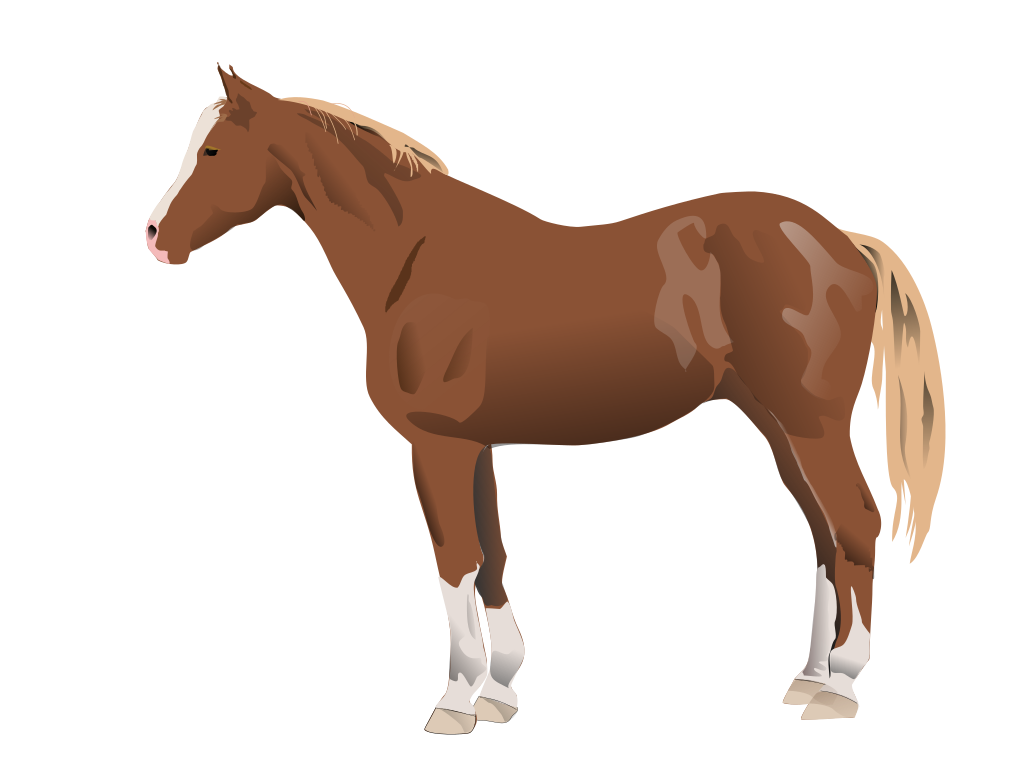
\includegraphics[width=\columnwidth]{Monsters/Animals/Horse, Riding}

\subsection{Horse, War}\index[monsters]{War Horse}
\statblock{\textbf{Size:} Large

\textbf{Type:} Animal

\textbf{Habitat:} Clear (Common)

\textbf{Wandering Group:} 0 (Nil)

\textbf{Lair Group:} 0 (Nil)

\textbf{Move:} 80 ft.

\textbf{Armor Class:} 7

\textbf{Hit Dice:} 3 (14 HP)

\textbf{Attacks:} 2x Kick (1d6)

\textbf{Special:} Charge

\textbf{Save:} F2

\textbf{Alignment:} None

\textbf{Intelligence:} 2

\textbf{Morale:} 9

\textbf{XP Value:} 20}

War horses are strong, heavy horses bred for their courage and willingness to fight.

They are purely a domesticated breed, and do not exist in the wild.

\textbf{Charge:} War horses can do the Charge action in combat, but cannot attack at the end of it. However, if a war horse does a Charge action then its rider gets the double-damage benefit.

Anyone using the Set Spear action against a charging war horse can choose to either hit the horse or its rider.

\subsection{Hsiao}\index[monsters]{Hsiao}
\monsterimage{Monsters/Hsiao}{\statblock{\textbf{Size:} Large

\textbf{Type:} Monster

\textbf{Habitat:} Woods (Rare)

\textbf{Wandering Group:} 1d4 (Nil)

\textbf{Lair Group:} 1d20 (O)

\textbf{Move:} 30 ft., 70 ft. (Fly)

\textbf{Armor Class:} 5

\textbf{Hit Dice:} 10****

\textbf{Attacks:} 2x Claw (1d6) or Beak (1d4)

\textbf{Special:} Cleric Abilities

\textbf{Save:} C10

\textbf{Alignment:} Lawful

\textbf{Intelligence:} 10

\textbf{Morale:} 9

\textbf{XP Value:} 4,000}}

Hsiao are giant owl-like creatures with large eyes and broad feathered wings.

Hsiao live in tall trees where they make earthern nests and tunnels.

Hsiao are peaceful philosophers who protect the wilderness from those that would do it harm. They work closely with other woodland creatures and may call on them for aid.

\textbf{Cleric Abilities:} Hsiao can use all \iref[class:Cleric]{Cleric} abilities as a \iref[class:Cleric]{Cleric} of 4 levels higher.

\subsubsection{As a Class}\index[classes]{Hsiao}
Hsiao can be used as a class using the following statistics:

\statblock{\textbf{Ability Requirements:} Intelligence 6, Wisdom 8

\textbf{Prime Requisite:} Wisdom

\textbf{Ability Modifiers:} None

\textbf{Weapons:} Strength -1, Wisdom +1

\textbf{Natural Attacks:} Unchanged (Level -3: 1d2/1d2/1d2, Level -2: 1d3/1d3/1d2, Level -1: 1d4/1d4/1d3, Level 0+: 1d6/1d6/1d4)

\textbf{Armor:} Leather Armor (4 AC, 200 gp, 100 cn)

\textbf{Natural AC:} 8 (Level -3), 7 (Level -2), 6 (Level -1), 5 (Level 0+)

\textbf{Special Abilities:} Cleric Abilities

\textbf{Magic Item Use:} Cleric}

\begin {table}[H]
  \caption{Hsiao Progression}
  \begin{tabularx}{\columnwidth}{>{\bfseries}YYY}
	\thead{Level} & \thead{Experience} & \thead{Hit Dice}\\
	-3 & -8,000 & 1d8\\
	-2 & -6,000 & 2d8\\
	-1 & -4,000 & 3d8\\
	0 & 0 & 4d8\\
	1 & 8,000 & 5d8\\
	2 & 24,000 & 6d8\\
	3 & 56,000 & 7d8\\
	4 & 115,000 & 8d8\\
	5 & 250,000 & 9d8\\
	6 & 500,000 & 10d8\\
	7 & 800,000 & 11d8\\
	8 & 1,100,000 & 12d8\\
	9 & 1,400,000 & 13d8\\
	10 & 1,700,000 & 14d8\\
	11 & 2,000,000 & 15d8\\
	12+ & +300,000 & +1 HP
  \end {tabularx}
\end {table}

\subsection{Human, Bandit}\index[monsters]{Human Bandit}
\statblock{\textbf{Size:} Medium

\textbf{Type:} Human

\textbf{Habitat:} Any (Common)

\textbf{Wandering Group:} 2d4 (U)

\textbf{Lair Group:} 2d10 (A)

\textbf{Move:} 30 ft.

\textbf{Armor Class:} 6

\textbf{Hit Dice:} 1 (5 HP)

\textbf{Attacks:} Weapon (By weapon)

\textbf{Special:} None/Leader (As Class)

\textbf{Save:} R1

\textbf{Alignment:} Any

\textbf{Intelligence:} 11

\textbf{Morale:} 8

\textbf{XP Value:} 10}

The statistics given here are for typical sorts of robbers such as bandits, brigands, buccaneers, and pirates. Bandit leaders are likely to be higher level characters with the same classes and abilities that player characters have.

\subsection{Human, Commoner}\index[monsters]{Human Commoner}
\statblock{\textbf{Size:} Medium

\textbf{Type:} Human

\textbf{Habitat:} Any (Common)

\textbf{Wandering Group:} 1d4 (P)

\textbf{Lair Group:} 3d20 (U)

\textbf{Move:} 40 ft.

\textbf{Armor Class:} 9

\textbf{Hit Dice:} 1-1 (4 HP)

\textbf{Attacks:} Weapon (By weapon)

\textbf{Special:} None

\textbf{Save:} F0

\textbf{Alignment:} Any

\textbf{Intelligence:} 10

\textbf{Morale:} 6

\textbf{XP Value:} 5}

The statistics given here are for a normal human with no combat experience, such as peasants, artists, servants or townsfolk.

\subsection{Human, Noble}\index[monsters]{Human Noble}
\statblock{\textbf{Size:} Medium

\textbf{Type:} Human

\textbf{Habitat:} Any (Common)

\textbf{Wandering Group:} 1 (Vx3)

\textbf{Lair Group:} 2d6 (D+B)

\textbf{Move:} 20 ft.

\textbf{Armor Class:} 2

\textbf{Hit Dice:} 5* (23 HP)

\textbf{Attacks:} Weapon (By weapon)

\textbf{Special:} None

\textbf{Save:} F5

\textbf{Alignment:} Any

\textbf{Intelligence:} 10

\textbf{Morale:} 8

\textbf{XP Value:} 400}

These statistics are for a minor non-landed noble such as a knight. Such a noble will have extensive combat training, but little practical experience.

More experienced nobles who are in charge of fiefdoms and are proven in battle are likely to be at least \nth{9} level characters with the same classes and abilities that player characters have.

\subsection{Human, Nomad}\index[monsters]{Human Nomad}
\statblock{\textbf{Size:} Medium

\textbf{Type:} Human

\textbf{Habitat:} Any (Common)

\textbf{Wandering Group:} 1 (P)

\textbf{Lair Group:} 4d10 (A)

\textbf{Move:} 40 ft.

\textbf{Armor Class:} 8

\textbf{Hit Dice:} 1 (4 HP)

\textbf{Attacks:} Weapon (By weapon)

\textbf{Special:} None

\textbf{Save:} F1

\textbf{Alignment:} None

\textbf{Intelligence:} 11

\textbf{Morale:} 8

\textbf{XP Value:} 10}

The statistics given here are for wandering tribesmen. They are fervent traders and usually have various knowledge about other lands.

\subsection{Human, Trader}\index[monsters]{Human Trader}
\statblock{\textbf{Size:} Medium

\textbf{Type:} Human

\textbf{Habitat:} Any (Common)

\textbf{Wandering Group:} 1 (U)

\textbf{Lair Group:} 1d20 (A)

\textbf{Move:} 30 ft.

\textbf{Armor Class:} 5

\textbf{Hit Dice:} 1 (4 HP)

\textbf{Attacks:} Weapon (By weapon)

\textbf{Special:} None

\textbf{Save:} F1

\textbf{Alignment:} None

\textbf{Intelligence:} 11

\textbf{Morale:} 7

\textbf{XP Value:} 10}

The statistics given here are for merchants that travel from town to town in caravans buying and selling various goods.

\subsection{Human, Veteran}\index[monsters]{Human Veteran}
\statblock{\textbf{Size:} Medium

\textbf{Type:} Human

\textbf{Habitat:} Any (Common)

\textbf{Wandering Group:} 2d4 (U)

\textbf{Lair Group:} 4d10 (A)

\textbf{Move:} 30 ft.

\textbf{Armor Class:} 6

\textbf{Hit Dice:} 2 (9 HP)

\textbf{Attacks:} Weapon (By weapon)

\textbf{Special:} None/Leader (As Class)

\textbf{Save:} F1

\textbf{Alignment:} Any

\textbf{Intelligence:} 11

\textbf{Morale:} 10

\textbf{XP Value:} 20}

These statistics can be used for squads of soldiers or mercenary companies who have seen plenty of real action (as opposed to merely training) and are somewhat battle-hardened.

The leaders of such groups are likely to be higher level characters, usually fighters, with the same classes and abilities that player characters have.

\subsection{Hydra}\index[monsters]{Hydra}
\statblock{\textbf{Size:} Large

\textbf{Type:} Dragon

\textbf{Habitat:} Swamp (Rare)

\textbf{Wandering Group:} 1 (Nil)

\textbf{Lair Group:} 1 (B)

\textbf{Move:} 40 ft.

\textbf{Armor Class:} 5

\textbf{Hit Dice:} Varies

\textbf{Attacks:} Varies

\textbf{Special:} None

\textbf{Save:} Varies

\textbf{Alignment:} None

\textbf{Intelligence:} 2

\textbf{Morale:} 11

\textbf{XP Value:} Varies}

Hydras are creatures with snake-like bodies that split into between 5 and 12 necks and heads. See \fullref{tab:Hydra Abilities by Number of Heads} for the statistics of hydras that vary by number of heads.

Each head of a hydra can operate independently, and can make a single bite attack in combat for 1d10 damage.

Damage to a hydra’s heads is not tracked independently, but for each 8 damage that the hydra takes from any source, one head will cease to function and no longer be able to attack.

Hydras are very territorial and aggressive creatures, and will attack any who approach the swamp or lake where they live.

\begin {table}[H]
  \caption{Hydra Abilities by Number of Heads}\label{tab:Hydra Abilities by Number of Heads}
  \begin{tabularx}{\columnwidth}{>{\bfseries}cYYY}
	\thead{Number of Heads} & \thead{Hit Dice} & \thead{Save} & \thead{XP}\\
	5 & 5 (23 HP) & F5 & 175\\
	6 & 6 (27 HP) & F6 & 275\\
	7 & 7 (32 HP) & F7 & 450\\
	8 & 8 (36 HP) & F8 & 650\\
	9 & 9 (41 HP) & F9 & 900\\
	10 & 10 (45 HP) & F10 & 1,000\\
	11 & 11 (50 HP) & F11 & 1,100\\
	12 & 12 (54 HP) & F12 & 1,250
  \end {tabularx}
\end {table}

\subsubsection{Flying Hydra}\index[monsters]{Flying Hydra}
Flying hydras have huge bat-like wings which allow them to fly at 60 feet per round. Their hit dice are 5-9*.

\textbf{Swoop:} Flying hydras can swoop down on an opponent and either attack them or carry them off if they are human-sized or smaller. Up to three heads can perform these actions when swooping.

\subsubsection{Regenerating Hydra}\index[monsters]{Regenerating Hydra}
\textbf{Regeneration:} Regenerating hydras regenerate 3 hit points per round until slain. Damage from fire cannot be regenerated.

\subsubsection{Sea Hydra}\index[monsters]{Sea Hydra}
Sea hydras can breath underwater and have fins instead of legs.

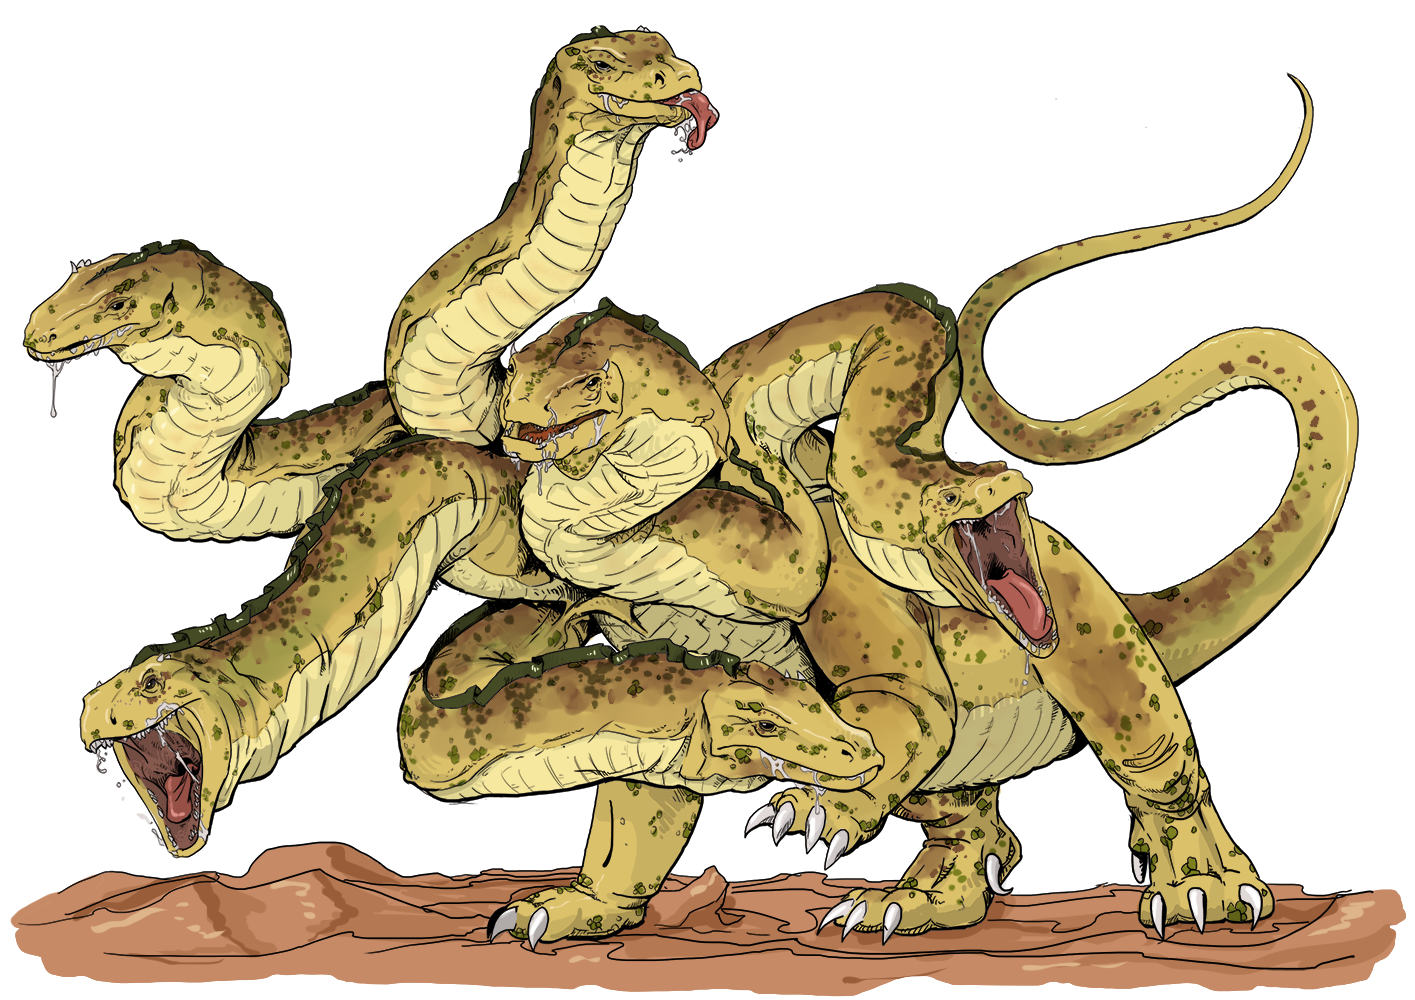
\includegraphics[width=\columnwidth]{Monsters/Hydra}

\subsection{Imp, Wood}\index[monsters]{Wood Imp}
\statblock{\textbf{Size:} Small

\textbf{Type:} Humanoid

\textbf{Habitat:} Woods (Rare)

\textbf{Wandering Group:} 1d4 (S)

\textbf{Lair Group:} 8d10 (C+N)

\textbf{Move:} 30 ft.

\textbf{Armor Class:} 6

\textbf{Hit Dice:} 3/4* (3 HP)

\textbf{Attacks:} Bite (1d3), Weapon (By Weapon)

\textbf{Special:} Camouflage, Poison Arrow

\textbf{Save:} F0

\textbf{Alignment:} Chaotic

\textbf{Intelligence:} 15

\textbf{Morale:} 7 or 9

\textbf{XP Value:} 725}

Wood imps are small humanoids with green skin and wild tangled hair; usually with twigs and leafs stuck in it. They have a round face with a wide mouth containing needle-shaped teeth.

Wood imps are protective of their territory. They will hunt intruders and lay traps for them. When hunting, wood imps ride a \iref[Huge Wood Spider]{Huge Wood Spider}. Rather than attacking directly, wood imps prefer to lure the intruders into their traps where the victim is captured or slain by the wood imp's poison arrow.

\textbf{Camouflage:} The wood imp's green skin provide remarkably effective camouflage in wooded surroundings, causing the wood imp to surprise their opponents on a 1-3 on 1d6.

\textbf{Poison Arrow:} Wood imps may spend 1 round extracting poison from their huge wood spider mount and coating their arrows with it. Anyone struck by these poison arrows must make a saving throw vs. poison with a +2 bonus or suffer 1d8 points of damage and become \iref[sec:Sluggish]{Sluggish} for 2d4+2 rounds. The poison arrows must be used the round after it was extracted or the poison evaporates. Poison from a dead huge wood spider is inefective.

\subsubsection{Spellcasting}
Wood imps can be shamans (to \nth{4} level).

\subsubsection{As a Class}\index[classes]{Wood Imp}
Wood imps can be used as a class using the following statistics:

\statblock{\textbf{Ability Requirements:} Strength 6, Dexterity 6

\textbf{Prime Requisite:} Dexterity

\textbf{Ability Modifiers:} None

\textbf{Weapons:} Any

\textbf{Armor:} Any

\textbf{Natural AC:} 8

\textbf{Special Abilities:} Camouflage

\textbf{Magic Item Use:} Fighter}

\begin {table}[H]
  \caption{Wood Imp Progression}
  \begin{tabularx}{\columnwidth}{>{\bfseries}YYY}
		\thead{Level} & \thead{Experience} & \thead{Hit Dice}\\
	0 & 0 & 1d4\\
	1 & 800 & 2d4\\
	2 & 1,600 & 3d4\\
	3 & 3,200 & 3d4\\
	4 & 6,400 & 4d4\\
	5 & 12,800 & 5d4\\
	6 & 25,000 & 6d4\\
	7 & 50,000 & 7d4\\
	8 & 100,000 & 8d4\\
	9 & 200,000 & 9d4\\
	10 & 360,000 & 10d4\\
	11+ & +160,000 & +2 HP
  \end {tabularx}
\end {table}

\subsection{Insect Swarm}\index[monsters]{Insect Swarm}
\statblock{\textbf{Size:} Small

\textbf{Type:} Animal

\textbf{Habitat:} Any (Rare)

\textbf{Wandering Group:} 1 (Nil)

\textbf{Lair Group:} 1d3 (Nil)

\textbf{Move:} 10 ft., 20 ft. (Fly)

\textbf{Armor Class:} 7

\textbf{Hit Dice:} 2* (9 HP)

\textbf{Attacks:} Special

\textbf{Special:} None

\textbf{Save:} F0

\textbf{Alignment:} None

\textbf{Intelligence:} 0

\textbf{Morale:} 11

\textbf{XP Value:} 25}

An insect swarm is a multitude of tiny insects acting as a single creature. Some insects swarm naturally, but others only swarm when commanded by the magical power of another creature.

A swarm fills a 10-by-10-by-30-foot area, and automatically hits any creature in the area each round for 2 points of damage (if the creature is AC 5 or better) or 4 damage (if the creature is AC 6 or worse). This damage represents many stings and bites.

Any creature in the area whose action for the round is either to run from the area or to swat the insects with a weapon or torch will take only 1 damage.

Attacking the swarm by swatting insects with a melee weapon will only do a single point of damage to it. Swarms are not harmed by missile weapons. Fire and cold attacks or area effect attacks do full damage to a swarm.

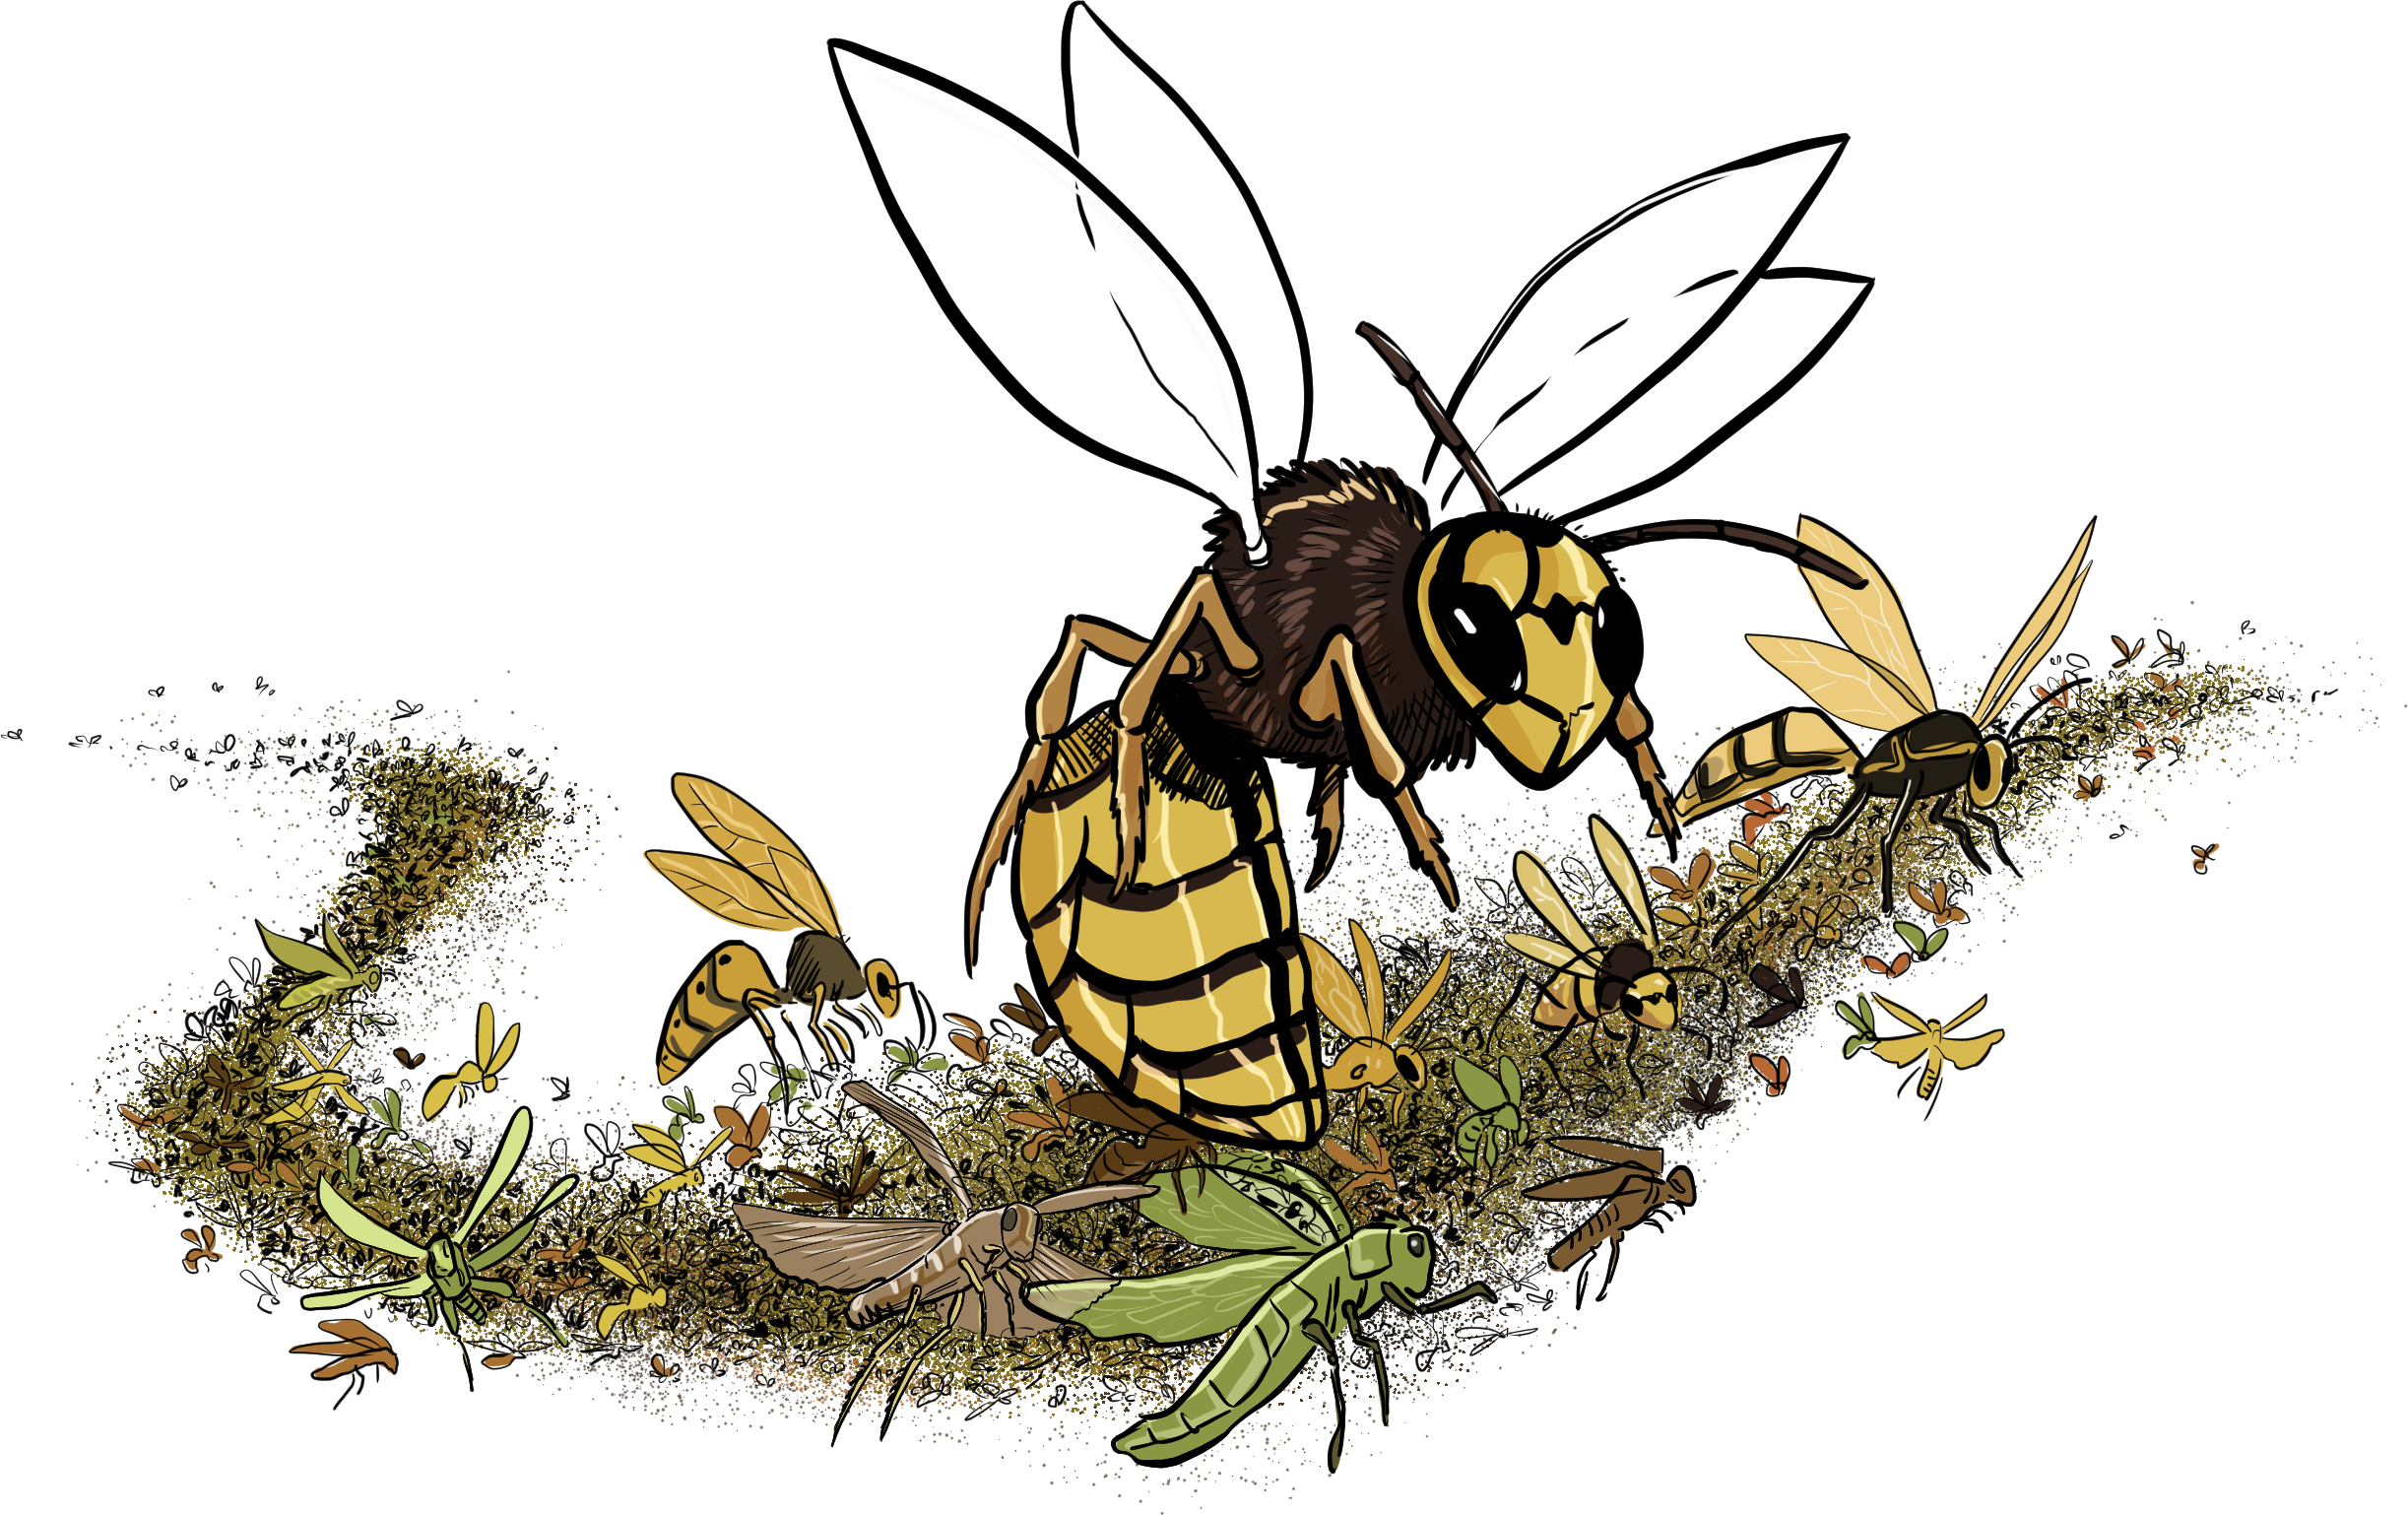
\includegraphics[width=\columnwidth]{Monsters/Animals/Insect Swarm}

\subsection{Invisible Stalker}\index[monsters]{Invisible Stalker}\label{sec:Invisible Stalker}
\begin {table}[H]
  \normalsize
  \begin{tabularx}{\columnwidth}{>{\bfseries}llX}
  \hiderowcolors
	& \textbf{Prime Plane} & \textbf{Home Plane}\\
	Size: & Medium & Medium\\
	Type: & Extraplanar & Extraplanar\\
	Habitat: & Any & Elemental Plane of Air (Rare)\\
	Wandering Group: & 1 (Nil) & 1 (Nil)\\
	Lair Group: & 0 (Nil) & 0 (Nil)\\
	Move: & 40 ft. & 120 ft.\\
	Armor Class: & 7 & 7\\
	Hit Dice: & 8* (36 HP) & 1-12 HD* (5-54 HP)\\
	Attacks: & Bash (4d4) & Bash ((HD/2)d4)\\
	Special: & Natural & ESP, Shapeshift\\
					 & Invisibility &\\
	Save: & F8 & F(HD)\\
	Alignment: & Neutral & Neutral\\
	Intelligence: & 11 & 11\\
	Morale: & 12 & 12\\
	XP Value: & 1,200 & By HD (see \fullref{tab:Base Monster Abilities})\\
  \showrowcolors
  \end {tabularx}
\end {table}

Invisible stalkers are extraplanar creatures that appear to be roughly humanoid in shape with a curiously “melted” appearance.

Invisible stalkers are often summoned to the prime plane to perform tasks. They hate such service, and will often try to go against the spirit of their instructions to the detriment of the person summoning them, while still being forced to obey the letter of them.

\textbf{Natural Invisibility:} Their natural invisibility allows the invisible stalker to surprise opponents on a roll of 1-5 on 1d6, unless those opponents can see invisible creatures.

\subsubsection{Home Plane}
Invisible stalkers originate from the Elemental Plane of Air. When on that plane their true form is nearly identical to an air elemental.

\textbf{ESP:} Invisible stalkers can use ESP at will as the spell \iref[spell:ESP]{ESP}.

\textbf{Shapechange:} Invisible stalkers can change shape at will into any creature native to the Elemental Plane of Air.

\subsection{Iron Urchin}\index[monsters]{Iron Urchin}
\statblock{\textbf{Size:} Medium

\textbf{Type:} Monster

\textbf{Habitat:} Elemental Plane of Earth (Very Rare)

\textbf{Wandering Group:} 1d6 (Nil)

\textbf{Lair Group:} 10d100 (Nil)

\textbf{Move:} 80 ft.

\textbf{Armor Class:} 2*

\textbf{Hit Dice:} 9* (41 HP)

\textbf{Attacks:} 3x Spike (1d12)

\textbf{Special:} Immunity (Normal Weapons, 

Poison, Spells < \nth{3} level), Spell-like Abilities

\textbf{Save:} E9

\textbf{Alignment:} Lawful

\textbf{Intelligence:} 10

\textbf{Morale:} 9

\textbf{XP Value:} 1,600}

Iron urchins have the appearance of a central ball 2 feet in diameter surrounded on all sides by 3-foot spikes, all made of iron.

An iron urchin has no visible sensory organs, mouth or other features, and feeds by absorbing mineral nutrients directly from the earth through its skin. They communicate solely by telepathy, and are usually friendly to outsiders unless provoked.

\textbf{Spell-like Abilities:} An iron urchin can cast the following spells as if a \nth{9} level caster: \iref[spell:Detect Invisible]{Detect Invisible} (at will), \iref[spell:Detect Magic]{Detect Magic} (at will), \iref[spell:Haste]{Haste} (at will), \iref[spell:Detect Magic]{Detect Magic} (at will), \iref[spell:Ice Storm/Wall of Ice]{Ice Storm/Wall of Ice} (at will), \iref[spell:Earth to Air]{Earth to Air} (3/day), and \ilink{spell:Air to Earth}{Air to Earth} (3/day).

\subsection{Kobold}\index[monsters]{Kobold}
\monsterimage{Monsters/Kobold}{\statblock{\textbf{Size:} Small

\textbf{Type:} Humanoid

\textbf{Habitat:} Hills, Mountains,

Underground, Woods (Common)

\textbf{Wandering Group:} 4d4 (P)

\textbf{Lair Group:} 6d10 (J)

\textbf{Move:} 30 ft.

\textbf{Armor Class:} 7

\textbf{Hit Dice:} 1/2 (3 HP)

\textbf{Attacks:} Weapon (By weapon - 1)

\textbf{Special:} Infravision

\textbf{Save:} F0

\textbf{Alignment:} Chaotic

\textbf{Intelligence:} 5

\textbf{Morale:} 9

\textbf{XP Value:} 5}}

Kobolds are hairless humanoids with heads shaped like those of hounds. Their skin is soft and dry like that of a snake, with patchy yellowish brown pigmentation. Kobolds do not have tails.

Kobolds have keen senses. Although not too bright in general, kobolds have an innate genius for trap building.

Kobolds usually live underground in clans in well guarded lairs. They are keen and gregarious, if unscrupulous and immoral, opportunists; easily convinced to work with other races on some common scheme.

Kobolds prefer not to fight at all, letting traps do the work for them. If forced to fight, their preferred method is ambush and hit-and-run tactics, combining surprising bravery with practical self-preservation.

\subsubsection{Spellcasting}
Kobolds can be shamans (to \nth{6} level) or sorcerers (to \nth{4} level).

\subsubsection{As a Class}\index[classes]{Kobold}
Kobolds can be used as a class using the following statistics:

\statblock{\textbf{Ability Requirements:} None

\textbf{Prime Requisite:} Strength, Dexterity, Intelligence, or Wisdom

\textbf{Ability Modifiers:} Strength -4, Dexterity +3

\textbf{Weapons:} Any small

\textbf{Armor:} Any except large shields

\textbf{Natural AC:} 7

\textbf{Special Abilities:} None

\textbf{Magic Item Use:} Fighter}

\begin {table}[H]
  \caption{Kobold Progression}
  \begin{tabularx}{\columnwidth}{>{\bfseries}YYY}
	\thead{Level} & \thead{Experience} & \thead{Hit Dice}\\
	0 & 0 & 1d4\\
	1 & 500 & 2d4\\
	2 & 1,000 & 3d4\\
	3 & 2,000 & 4d4\\
	4 & 4,000 & 5d4\\
	5 & 8,000 & 6d4\\
	6 & 16,000 & 7d4\\
	7 & 30,000 & 8d4\\
	8 & 60,000 & 9d4\\
	9 & 120,000 & 9d4+2\\
	10+ & +100,000 & +2 HP
  \end {tabularx}
\end {table}

\subsection{Leech, Giant}\index[monsters]{Giant Leech}
\statblock{\textbf{Size:} Small

\textbf{Type:} Animal

\textbf{Habitat:} Swamp (Common)

\textbf{Wandering Group:} 0 (Nil)

\textbf{Lair Group:} 1d4 (Nil)

\textbf{Move:} 30 ft.

\textbf{Armor Class:} 7

\textbf{Hit Dice:} 6 (27 HP)

\textbf{Attacks:} Bite (1d6)

\textbf{Special:} Drain Blood

\textbf{Save:} F3

\textbf{Alignment:} None

\textbf{Intelligence:} 0

\textbf{Morale:} 10

\textbf{XP Value:} 275}

Giant leeches are parasitic worm-like creatures that suck blood from prey larger than themselves.

\textbf{Drain Blood:} If a leech’s bite succeeds, it will hold on to that victim and begin to drain their blood. The victim suffers 1d6 points of damage for every round their blood is being drained. The leech will continue to drain the victim's blood until either the leech or the victim is dies.

\subsection{Leprechaun}\index[monsters]{Leprechaun}
\statblock{\textbf{Size:} Small

\textbf{Type:} Fey

\textbf{Habitat:} Woods (Rare)

\textbf{Wandering Group:} 1d10 (See Below)

\textbf{Lair Group:} 1 (See Below)

\textbf{Move:} 20 ft.

\textbf{Armor Class:} 5

\textbf{Hit Dice:} 1/4 (2 HP)

\textbf{Attacks:} Weapon (By weapon)

\textbf{Special:} Invisibility to Mortals

\textbf{Save:} E1

\textbf{Alignment:} Lawful

\textbf{Intelligence:} 14

\textbf{Morale:} 6

\textbf{XP Value:} 6}

Leprechauns are small humanoids with pointed ears. Their other psychical traits vary widely.

Leprechauns are the chief craftsmen of the fey, making things such as clothes, weapons, wine casks, and magical items. They trade these items to other fey for food, material, and treasure. Leprechaun loathe evil creatures and those that cause harm to their environment. They will ward of such creatures to the best of their ability.

\textbf{Invisibility to Mortals:} Leprechauns can not turn \iref[sec:Invisible]{Invisible} if a mortal is viewing them.

\subsubsection{As a Class}\index[classes]{Leprechaun}
Leprechauns can be used as a class using the following statistics:

\textbf{Fey Spells:} Leprechauns can cast fey spells. See \fullref{sec:Spell Descriptions} for detailed descriptions of these spells.

\statblock{\textbf{Ability Requirements:} Dexterity 9, Constitution 5, Intelligence 9

\textbf{Prime Requisite:} Dexterity and Intelligence

\textbf{Ability Modifiers:} Strength -2, Dexterity +2, Constitution -2, Charisma +2

\textbf{Weapons:} Daggers

\textbf{Armor:} None

\textbf{Natural AC:} 7

\textbf{Special Abilities:} Fey Spells, Invisibility to Mortals

\textbf{Magic Item Use:} All except Cleric}

\begin {table}[H]
  \caption{Leprechaun Progression}
  \begin{tabularx}{\columnwidth}{>{\bfseries}YYY}
	\thead{Level} & \thead{Experience} & \thead{Hit Dice}\\
	0 & 0 & 1d2\\
	1 & 2,000 & 1d4+1d2\\
	2 & 4,000 & 2d4\\
	3 & 8,000 & 3d4\\
	4 & 16,000 & 4d4\\
	5 & 32,000 & 5d4\\
	6 & 64,000 & 6d4\\
	7 & 130,000 & 7d4\\
	8 & 260,000 & 8d4\\
	9 & 520,000 & 9d4\\
	10 & 780,000 & 9d4\\
	11+ & +260,000 & +1 HP
  \end {tabularx}
\end {table}


\begin {table}[H]
  \caption{Leprechaun Spells per Day by Spell Level}
  \begin{tabularx}{\columnwidth}{>{\bfseries}YYYYYY}
	\thead{} & \multicolumn{5}{c}{\thead{Spell Level}}\\
	\thead{Level} & \thead{1} & \thead{2} & \thead{3} & \thead{4} & \thead{5}\\
	1 & 1 & - & - & - & -\\
	2 & 2 & - & - & - & -\\
	3 & 2 & 1 & - & - & -\\
	4 & 2 & 2 & - & - & -\\
	5 & 2 & 2 & 1 & - & -\\
	6 & 3 & 2 & 2 & - & -\\
	7 & 3 & 2 & 2 & 1 & -\\
	8 & 3 & 3 & 2 & 2 & -\\
	9 & 3 & 3 & 2 & 2 & 1\\
	10 & 4 & 3 & 3 & 2 & 2\\
	11 & 4 & 4 & 4 & 3 & 3\\
	12* & 4 & 4 & 4 & 4 & 4
  \end {tabularx}
	*Maximum level that spells may be obtained.
\end {table}

\subsection{Lich}\index[monsters]{Lich}
\statblock{\textbf{Size:} Medium

\textbf{Type:} Undead

\textbf{Habitat:} Any (Very Rare)

\textbf{Wandering Group:} 0 (Nil)

\textbf{Lair Group:} 1 (Hx4)

\textbf{Move:} 30 ft.

\textbf{Armor Class:} Varies

\textbf{Hit Dice:} Varies

\textbf{Attacks:} Touch (1d10+Special) or Weapon (By weapon) or Spell

\textbf{Special:} Cleric/Wizard Abilities, Despair, Immunity (Cold, 

Death Spells, Lightning, Mind Effects, Normal Weapons, Poison, 

Polymorph, Spells < \nth{4} level), Paralyzing Touch, Summon Undead

\textbf{Save:} Varies

\textbf{Alignment:} Varies

\textbf{Intelligence:} 18+

\textbf{Morale:} 10

\textbf{XP Value:} Varies}

A lich is a human cleric or wizard who has used a forbidden arcane ritual to turn themselves into an undead creature. Although theoretically a lich can have any personality and alignment, it is normally only the most depraved or desperate individuals who are willing to perform the ritual.

A lich’s skeletal form is armor class 0 (unless wearing better armor).

Because liches are so intelligent, the Game Master should put thought and preparation into their motivations and tactics, in particular the potential for them to have cast the Permanence and Contingency spells on themselves. A lich will not simply be randomly encountered and get into a pointless fight where it has a chance of dying.

A lich will be accompanied by undead minions that it controls as an Undead Liege, and often by other servants or minions.

A lich is treated as if it had hit dice equal to its level for the purposes of experience value, plus the equivalent of five asterisks if a cleric, or six if a wizard.

\textbf{Cleric/Wizard Abilities:} A lich will have all the abilities of a cleric or wizard of level 21 or higher.

\textbf{Despair:} Any living creature with fewer than 5 hit dice will flee in terror (no saving throw) from a lich for 2d6 rounds.

\textbf{Paralyzing Touch:} The touch of a lich does 1d10 cold damage and paralyzes any living creature for 1d100 days unless the creature can make a saving throw vs. paralysis. The paralysis can be removed by a Dispel Magic spell.

\textbf{Summon Undead:} A lich can summon undead by concentrating although it does not know what type of undead will turn up. Each time a lich summons undead, refer to \fullref{tab:Lich} to determine randomly what type of undead arrive in 1d100 rounds.

\begin {table}[H]
	\caption{Lich}\label{tab:Lich}
  \begin{tabularx}{\columnwidth}{>{\bfseries}YY}
	\thead{1d20} & \thead{Type}\\
	1-5 & 2d4 Spectres\\
	6-9 & 1d6 Vampires\\
	10-12 & 1d3 Phantoms\\
	13-15 & 1d2 Ghosts\\
	16 & 1d2 Poltergeists\\
	17 & 1 Druj\\
	18 & 1 Revenant\\
	19 & 1 Nightshade\\
	20 & 1 Undead Gazer
  \end {tabularx}
\end {table}

\subsection{Living Statue}
Living statues are constructs made from a humanoid figure sculpted from a specific material. A stationary living statue cannot be distinguished from a statue made of the same material as them.

Living statues are the most commonly encountered type of construct, and are somewhat more intelligent than most other constructs, and while unable to speak; they are able to follow more complex orders.

\subsubsection{Living Crystal Statue}\index[monsters]{Living Crystal Statue}
\statblock{\textbf{Size:} Medium

\textbf{Type:} Construct

\textbf{Habitat:} Any (Common)

\textbf{Wandering Group:} 1d6 (Nil)

\textbf{Lair Group:} 1d6 (Nil)

\textbf{Move:} 30 ft.

\textbf{Armor Class:} 4

\textbf{Hit Dice:} 3 (14 HP)

\textbf{Attacks:} 2x Bash (1d6)

\textbf{Special:} Immunity (Mind Effects, Poison)

\textbf{Save:} F3

\textbf{Alignment:} Lawful

\textbf{Intelligence:} 7

\textbf{Morale:} 11

\textbf{XP Value:} 35}

Living crystal statues are made up of crystals.

\subsubsection{Living Iron Statue}\index[monsters]{Living Iron Statue}
\statblock{\textbf{Size:} Large

\textbf{Type:} Construct

\textbf{Habitat:} Any (Common)

\textbf{Wandering Group:} 1d4 (Nil)

\textbf{Lair Group:} 1d4 (Nil)

\textbf{Move:} 10 ft.

\textbf{Armor Class:} 2*

\textbf{Hit Dice:} 4* (18 HP)

\textbf{Attacks:} 2x Bash (1d8)

\textbf{Special:} Absorb Weapon, Immunity (Mind Effects, Poison)

\textbf{Save:} F4

\textbf{Alignment:} Neutral

\textbf{Intelligence:} 7

\textbf{Morale:} 11

\textbf{XP Value:} 125}

Living iron statues are made up of iron and steel.

\textbf{Absorb Weapon:} When a living iron statue is struck with a non-magical metal weapon, the attacker must make a saving throw vs. spells or the weapon will be become stuck in the golem. A stuck weapon can not be removed until the statue is destroyed. Should the statue not be destroyed, the weapon will be absorbed into the statue’s body over a period of time.

\subsubsection{Living Stone Statue}\index[monsters]{Living Stone Statue}
\statblock{\textbf{Size:} Large

\textbf{Type:} Construct

\textbf{Habitat:} Any (Common)

\textbf{Wandering Group:} 1d3 (Nil)

\textbf{Lair Group:} 1d3 (Nil)

\textbf{Move:} 20 ft.

\textbf{Armor Class:} 4

\textbf{Hit Dice:} 5* (23 HP)

\textbf{Attacks:} 2x Squirt (2d6) or 2x Bash (2d6)

\textbf{Special:} Immunity (Mind Effects, Poison), Magma Shot

\textbf{Save:} F5

\textbf{Alignment:} Chaotic

\textbf{Intelligence:} 7

\textbf{Morale:} 11

\textbf{XP Value:} 300}

Living stone statues are made of stone.

\textbf{Magma Shot:} A living stone statue attacks by squirting magma from its fingertips at opponents within 20 feet, or simply bashing those that come within melee range.

\subsection{Lizard, Giant Draco}\index[monsters]{Giant Draco Lizard}
\statblock{\textbf{Size:} Medium

\textbf{Type:} Animal

\textbf{Habitat:} Desert, Underground, Woods (Common)

\textbf{Wandering Group:} 1d4 (U)

\textbf{Lair Group:} 1d8 (Nil)

\textbf{Move:} 40 ft., 50 ft. (Glide)

\textbf{Armor Class:} 5

\textbf{Hit Dice:} 4+2 (20 HP)

\textbf{Attacks:} Bite (1d10)

\textbf{Special:} Glide

\textbf{Save:} F3

\textbf{Alignment:} None

\textbf{Intelligence:} 2

\textbf{Morale:} 7

\textbf{XP Value:} 125}

Giant draco lizards are 6 foot long carnivorous lizards with flaps of skin between their front and rear legs that let them glide through the air.

\textbf{Glide:} Giant draco lizard may leap out of tall trees and glide down at their prey. The initial glide attack should be treated as a Charge action.

\subsection{Lizard, Giant Gecko}\index[monsters]{Giant Gecko}
\statblock{\textbf{Size:} Medium

\textbf{Type:} Animal

\textbf{Habitat:} Desert, Underground, Woods (Common)

\textbf{Wandering Group:} 1d6 (U)

\textbf{Lair Group:} 1d10 (Nil)

\textbf{Move:} 40 ft.

\textbf{Armor Class:} 5

\textbf{Hit Dice:} 3+1 (15 HP)

\textbf{Attacks:} Bite (1d8)

\textbf{Special:} Seta

\textbf{Save:} F2

\textbf{Alignment:} None

\textbf{Intelligence:} 2

\textbf{Morale:} 7

\textbf{XP Value:} 50}

Giant geckos are 5 carnivorous lizards that hunt halfling sized or smaller creatures by climbing up above them and dropping on them.

\textbf{Seta:} Giant geckos have sticky pads on their feet that allow them to walk on any surface, including smooth glass walls and ceiling.

\subsection{Lizard, Giant Horned}\index[monsters]{Giant Horned Lizard}
\statblock{\textbf{Size:} Large

\textbf{Type:} Animal

\textbf{Habitat:} Desert, Underground, Woods (Common)

\textbf{Wandering Group:} 2d4 (U)

\textbf{Lair Group:} 1d6 (Nil)

\textbf{Move:} 40 ft.

\textbf{Armor Class:} 2

\textbf{Hit Dice:} 5* (23 HP)

\textbf{Attacks:} Bite (2d4) \& Horn (1d6)

\textbf{Special:} Tongue Grab

\textbf{Save:} F3

\textbf{Alignment:} None

\textbf{Intelligence:} 2

\textbf{Morale:} 7

\textbf{XP Value:} 300}

Giant horned lizards can change color to match their surroundings, surprising prey on a 1-5 on 1d6.

Horned lizards favor hunting giant insects, but will hunt other creatures if hungry.

\textbf{Tongue Grab:} Horned lizards can shoot their tongues 10 feet and anything human-sized or smaller hit by the tongue will be dragged into the lizard's mouth and automatically bitten.

\subsection{Lizard, Giant Tuatara}\index[monsters]{Giant Tuatara}
\statblock{\textbf{Size:} Large

\textbf{Type:} Animal

\textbf{Habitat:} Desert, Underground, Woods (Common)

\textbf{Wandering Group:} 1d2 (V)

\textbf{Lair Group:} 1d4 (Nil)

\textbf{Move:} 30 ft.

\textbf{Armor Class:} 4

\textbf{Hit Dice:} 6 (27 HP)

\textbf{Attacks:} 2x Claw (1d4) \& Bite (1d6)

\textbf{Special:} Infravision

\textbf{Save:} F3

\textbf{Alignment:} None

\textbf{Intelligence:} 2

\textbf{Morale:} 6

\textbf{XP Value:} 275}

Giant tuatara lizards are heavily built lizards with lumpy armored skin. They look somewhat like elongated toads.

Tuatara hunt at night.

\subsection{Lizardfolk}\index[monsters]{Lizardfolk}
\statblock{\textbf{Size:} Medium

\textbf{Type:} Humanoid

\textbf{Habitat:} River, Swamp, Underground (Common)

\textbf{Wandering Group:} 2d4 (Nil)

\textbf{Lair Group:} 6d6 (D)

\textbf{Move:} 20 ft., 40 ft. (Swim)

\textbf{Armor Class:} 5

\textbf{Hit Dice:} 2+1

\textbf{Attacks:} Weapon (By weapon + 1)

\textbf{Special:} Infravision

\textbf{Save:} F2

\textbf{Alignment:} Neutral

\textbf{Intelligence:} 6

\textbf{Morale:} 12

\textbf{XP Value:} 25}

Lizardfolk are humanoid crocodilians, often found in swamps or along rivers.

Although not particularly evil or intelligent, lizardfolk are cannibalistic and particularly like to eat any other intelligent humanoid if given the chance.

When swimming, lizardfolk look just like crocodiles.

Lizardfolk have a 30\% chance to hide while in a swamp.

Lizardfolk live a simple hunter-gatherer existence, and have no technology beyond a basic spear or club. Surprisingly, they don’t bite in combat. Although they have powerful jaws, their shape and stance prevents them from being effective in a fight while on land.

Lizardfolk often find themselves in uneasy truces with other races who provide them tributes of food (the only thing they value) in order to prevent them raiding.

\subsubsection{Spellcasting}
Lizardfolk can be shamans (to \nth{6} level) or sorcerers (to \nth{4} level).

\subsubsection{As a Class}\index[classes]{Lizardfolk}
Lizardfolk can be used as a class using the following statistics:

\textbf{Delayed Intellect:} When rolling for \iref[sec:Intelligence]{Intelligence}, Lizardfolk only roll a 1d4+2. Their \iref[sec:Intelligence]{Intelligence} score may not be enhanced by adjusting ability scores. When gaining a level the lizardfolk must roll an intelligence check. If the check fails, the lizardfolk gains one point of \iref[sec:Intelligence]{Intelligence}. Their \iref[sec:Intelligence]{Intelligence} may never be raised above eight in this way.

\statblock{\textbf{Ability Requirements:} Strength 8, Constitution 6

\textbf{Prime Requisite:} Strength

\textbf{Ability Modifiers:} None

\textbf{Weapons:} Any

\textbf{Armor:} Any

\textbf{Natural AC:} 7

\textbf{Special Abilities:} None

\textbf{Magic Item Use:} Fighter}

\begin {table}[H]
  \caption{Lizardfolk Progression}
  \begin{tabularx}{\columnwidth}{>{\bfseries}YYY}
  \thead{Level} & \thead{Experience} & \thead{Hit Dice}\\
	-1 & -1,200 & 1d8+1\\
	0 & 0 & 2d8+1\\
	1 & 1,200 & 3d8+2\\
	2 & 3,600 & 4d8+3\\
	3 & 8,400 & -\\
	4 & 18,000 & 5d8+3\\
	5 & 37,200 & 6d8+4\\
	6 & 75,600 & 7d8+4\\
	7 & 152,400 & -\\
	8 & 306,000 & 8d8+5\\
	9+ & +300,000 & +2 HP
  \end {tabularx}
\end {table}

\subsection{Locust, Giant}\index[monsters]{Giant Locust}
\statblock{\textbf{Size:} Small

\textbf{Type:} Animal

\textbf{Habitat:} Underground (Common)

\textbf{Wandering Group:} 2d10 (Nil)

\textbf{Lair Group:} 0 (Nil)

\textbf{Move:} 20 ft., 60 ft. (Jump)

\textbf{Armor Class:} 4

\textbf{Hit Dice:} 2** (9 HP)

\textbf{Attacks:} Bite (1d2) or 

Jump (1d4) or Special

\textbf{Special:} Spit

\textbf{Save:} F2

\textbf{Alignment:} None

\textbf{Intelligence:} 0

\textbf{Morale:} 5

\textbf{XP Value:} 30}

Giant locusts live underground and eat fungus and molds of all types. They are immune to poisons and the dissolving attacks of oozes.

Although giant locusts can give a nasty bite, they prefer to flee by jumping away from intruders. Unfortunately, their panicked jumping is 50\% likely to be straight at their targets, in which case they should roll a jump attack against a random target.

\textbf{Spit:} If cornered and unable to jump away, a giant locust will make a piercing scream, and spit a blob of goo at an attacker within 10 feet.

If it hits, the goo does no damage, but the attacker must make a saving throw vs. poison or be able to do nothing but retch for 10 minutes due to the smell. Once the 10 minutes has passed, the victim of the goo attack is used to the smell, but other characters coming within 5 feet of them are subject to the same retching unless they can make a saving throw vs. poison. Giant locust spittle can be washed off with water.

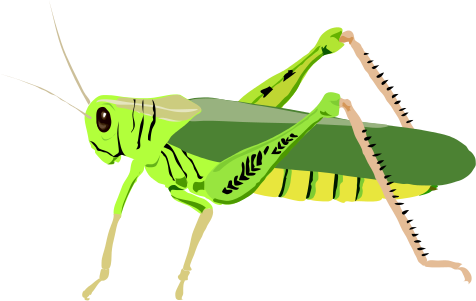
\includegraphics[width=\columnwidth]{Monsters/Animals/Locust, Giant}

\subsection{Lycanthrope}
A lycanthrope is a human suffering from lycanthropy, a magical disease which allows them change into a animal-like humanoid.

\textbf{Immunity to Non-Silver Weapons:} Lycanthropes are only hurt by silver weapons while in beast form.

\textbf{Lycanthropy:} Any human who loses more than half their hit points to a lycanthrope becomes a lycanthrope of the same type within 2d12 days. Non-humans who contract the disease are killed by it in the same time. Symptoms start to show after half the duration, and can only be cured by a Cure Disease cast by an \nth{11} level or higher caster.

\textbf{Summon Animals:} Lycanthropes can summon 1d2 animals of their type to help them once per day.

\textbf{Transform:} Lycanthropes can take two forms. Human form, which is their form before being inflicted with lycanthropy and beast form which is an animal-like humanoid.

\textit{Human Form:} After transforming into beast form, the lycanthrope automatically reverts to their human form at sunrise.

\textit{Beast Form:} During a full moon, the lycanthrope is forced to take their beast form. The lycanthrope can attempt to resist this change with a successful saving throw vs. spells with a -4 penalty if there is a full moon or a -2 penalty if its the day before or after a full moon.

Lycanthrope may also voluntarily take this form at any other time. When changing into beast form, all equipment carried by the lycanthrope drops to the ground and they are unable to use it while in this form. The lycanthrope can only speak and understand the language of their animal type. If the lycanthrope is a spellcaster, they forget all their prepared spells when taking this form.

\textbf{Vulnerability to Silver:} Lycanthropes are allergic to silver. If a lycanthrope is touching silver for more than one turn, than they break out into a painful rash unless they make a successful saving throw vs. poison.

\textbf{Vulnerability to Wolfsbane:} Lycanthrope are allergic to \iref[eq:Wolfsbane]{Wolfsbane}. If a lycanthrope touches it, they must make a saving throw vs. poison or run in fear for 2 turns as if effected by a \ilink{spell:Cause Fear}{Cause Fear} spell. 

\subsubsection{As a Class}
Lycanthrope can be used as a \iref[sec:Secondary Classes]{Secondary Class} with the following statistics:

Experience is only gained in this class while in beast form.

\textbf{Transform:} A lycanthrope can voluntarily change into beast form with a successful \iref[sec:Constitution]{Constitution} check with a +2 bonus if within a week of a full moon or a -2 penalty otherwise. This can be attempted once per hour and can only be done at night when the moon is shining. The transformation takes 15 minutes minus one for each level above -3 (minimum of 1 round).

Starting at level -2, a lycanthrope can voluntarily change into beast form at night without the moon.

Starting at level -1, a lycanthrope can voluntarily change into beast form at any time.

Starting at level 1, a voluntarily change can be attempted once per turn.

Starting at level 9, no \iref[sec:Constitution]{Constitution} check is required to change into beast form.

Starting at level 9, the lycanthrope's beast form becomes a hybrid form. In this form, the lycanthrope can use all abilities from both their human and beast form. When changing to this hybrid form, equipment is not dropped and can be used by the lycanthrope. Also, if they are a spellcaster, they do not forget their prepared spells.

\textbf{Resistance to Non-Silver Weapons:} Starting at level -2, lycanthropes only take half damage from normal weapons.

Starting at level -1, they take only 1/\nth{4} damage from normal weapons.

Starting at level 0, they do not take any damage from normal weapons.

\textbf{Speak With Animals:} Starting at level -2, a lycanthrope can speak with other lycanthropes and animals of their type while in beast form.

\textbf{Immunity to Non-Silver Weapons:} This ability is not gained until level 0.

\textbf{Summon Animals/Lycanthrope:} This ability is not gained until level 0. The amount of animals summoned increases with level: 1d4 at \nth{2}, 1d6 at \nth{4}, 1d8 at \nth{6}, and 1d8 at \nth{10}.

Starting at \nth{5} level, some of these summoned animals will instead be lycanthropes of the player's type. The amount of lycanthrope summoned is determined by the Game Master.

\textbf{Fast Healing:} Starting at \nth{3} level, a lycanthrope regains 1d4+1 hit points while resting in beast form for a full day. An additional hit point is regained for every three levels the lycanthrope has attained.

\subsubsection{Werebat}\index[monsters]{Werebat}
\statblock{\textbf{Size:} Medium

\textbf{Type:} Monster

\textbf{Habitat:} Underground (Common)

\textbf{Wandering Group:} 2d6 (Nil)

\textbf{Lair Group:} 1d8 (C)

\textbf{Move:} 20 ft., 60 ft. (Fly)

\textbf{Armor Class:} 4, 9 (Human)

\textbf{Hit Dice:} 3+3* (23 HP)

\textbf{Attacks:} Bite (1d4) or Weapon (By weapon)

\textbf{Special:} Cause Disease, Immunity to Charm, Immunity to Non-Silver Weapons, Lycanthropy, Summon Animals, Summon Werebats, Transform, Vulnerability to Silver, Vulnerability to Wolfsbane

\textbf{Save:} F3

\textbf{Alignment:} Chaotic

\textbf{Intelligence:} 10

\textbf{Morale:} 7

\textbf{XP Value:} 75}

Sometimes confused for vampires, these dangerous flying creatures can change form at will.

\textbf{Cause Disease:} When bitten by a werebat, there is a 1 in 6 chance that the victim will become inflicted with a non-magical disease (GM's choice).

\textbf{Summon Werebats:} Werebats can summon 1d4 other Werebats. These Werebats can't summon additional Werebats..

\paragraph{As a Class}\index[classes]{Werebat}\mbox{}\\
Werebats can be used as a class using the following statistics:

\textbf{Echolocation:} Werebats can find their way even in situations where they cannot see. By emitting ultrasonic squeaks and than listening for the echoes, the werebat can tell the dimensions of an enclosed space and their position within it. This will also reveal the size, outline, distance, and movement of all objects within 60 ft. of the werebat. Individuals can only be recognized this way if the werebat is within 10 ft of them and they are very distinctive.

\textbf{Shriek:} Starting at \nth{7} level, a werebat can emit a piercing scream for 1d3 rounds which can stun creatures and shatter glass within 120 yards.

All creatures within range must make saving throw vs. spells or become stunned for 1d6 rounds.

This ability may be used up to three times per day.

\textbf{Summon Werebats:} Werebats gain this ability at level 0.

\statblock{\textbf{Ability Requirements:} 

\textbf{Prime Requisite:} Strength

\textbf{Ability Modifiers:} Dexterity +1, Constitution +1, Charisma -2

\textbf{Weapons:} Special

\textbf{Armor:} Special

\textbf{Natural AC:} 7 (Level -3), 6 (Level -2), 5 (Level -1), 4 (Level 0+)

\textbf{Special Abilities:} 

\textbf{Magic Item Use:} Fighter}

\begin {table}[H]
  \caption{Werebat Progression}
  \begin{tabularx}{\columnwidth}{>{\bfseries}YYY}
  \thead{Level} & \thead{Experience} & \thead{Hit Dice}\\
	-3 & -6,400 & 1d8+1\\
	-2 & -3,200 & 2d8+2\\
	-1 & -1,600 & -\\
	0 & 0 & 3d8+3\\
	1 & 6,400 & 4d8+4\\
	2 & 19,200 & 5d8+5\\
	3 & 44,800 & -\\
	4 & 96,000 & 6d8+5\\
	5 & 198,400 & 7d8+5\\
	6 & 403,200 & 8d8+5\\
	7 & 700,000 & -\\
	8 & 1,000,000 & 9d8+5\\
	9+ & +300,000 & +2 HP
  \end {tabularx}
\end {table}

\subsubsection{Werebear}\index[monsters]{Werebear}
\statblock{\textbf{Size:} Large, Medium (Human)

\textbf{Type:} Monster

\textbf{Habitat:} Hills, Mountains, Woods (Common)

\textbf{Wandering Group:} 1d4 (Nil)

\textbf{Lair Group:} 1d4 (C)

\textbf{Move:} 40 ft.

\textbf{Armor Class:} 2, 8 (Human)

\textbf{Hit Dice:} 6* (27 HP)

\textbf{Attacks:} 2x Claw (2d4) \& Bite (1d8) or Weapon (By weapon)

\textbf{Special:} Hug, Immunity to Charm, Immunity to Non-Silver Weapons, Lycanthropy, Summon Animals, Transform, Vulnerability to Silver, Vulnerability to Wolfsbane

\textbf{Save:} F6

\textbf{Alignment:} Neutral

\textbf{Intelligence:} 10

\textbf{Morale:} 10

\textbf{XP Value:} 500}

Unlike most lycanthropes, werebears retain most of their intelligence and personality while in beast form, and can sometimes be reasoned with.

\textbf{Hug:} If both of a werebear’s claws hit the same target, the werebear can hug the target for an extra 2d8 damage.

\paragraph{As a Class}\index[classes]{Werebear}\mbox{}\\
Werebears can be used as a class using the following statistics:

\textbf{Plant Path:} Starting at \nth{7} level, a werebear can cause plants and trees in their path to bend or move aside. This ability can be used any number of times per day as long as the total rounds do not exceed the wearbear's level.

\statblock{\textbf{Ability Requirements:} 

\textbf{Prime Requisite:} Strength

\textbf{Ability Modifiers:} Strength +3, Dexterity -2, Constitution +2, Wisdom -2, Charisma -1

\textbf{Weapons:} Special

\textbf{Armor:} Special

\textbf{Natural Attacks:} Claw (1d4) or Bite (1d8) (Level -3), 2x Claw (2d4) \& Bite (1d8) (Level -2 and up)

\textbf{Natural AC:} 5 (Level -3), 4 (Level -2), 3 (Level -1), 2 (Level 0+)

\textbf{Special Abilities:} 

\textbf{Magic Item Use:} Fighter}

\begin {table}[H]
  \caption{Werebear Progression}
  \begin{tabularx}{\columnwidth}{>{\bfseries}YYY}
  \thead{Level} & \thead{Experience} & \thead{Hit Dice}\\
	-3 & -54,400 & 3d8\\
	-2 & -40,800 & 4d8\\
	-1 & -27,200 & 5d8\\
	0 & 0 & 6d8\\
	1 & 54,400 & 7d8\\
	2 & 163,200 & 8d8\\
	3 & 380,800 & -\\
	4 & 680,000 & 9d8\\
	5 & 980,000 & 10d8\\
	6 & 1,280,000 & 11d8\\
	7 & 1,580,000 & -\\
	8 & 1,880,000 & 12d8\\
	9+ & +300,000 & +2 HP
  \end {tabularx}
\end {table}

\subsubsection{Wereboar}\index[monsters]{Wereboar}
\statblock{\textbf{Size:} Medium

\textbf{Type:} Monster

\textbf{Habitat:} Woods (Common)

\textbf{Wandering Group:} 1d4 (Nil)

\textbf{Lair Group:} 2d4 (C)

\textbf{Move:} 50 ft.

\textbf{Armor Class:} 4, 9 (Human)

\textbf{Hit Dice:} 4+1* (19 HP)

\textbf{Attacks:} Gore (2d6) or Weapon (By weapon)

\textbf{Special:} Immunity to Charm (Animal), Immunity to Non-Silver Weapons, Lycanthropy, Summon Animals, Transform, Vulnerability to Silver, Vulnerability to Wolfsbane

\textbf{Save:} F4

\textbf{Alignment:} Neutral

\textbf{Intelligence:} 10

\textbf{Morale:} 9

\textbf{XP Value:} 200}

Wereboars are very belligerent and aggressive, even in human form. In human form they act as berserkers.

\paragraph{As a Class}\index[classes]{Wereboar}\mbox{}\\
Wereboars can be used as a class using the following statistics:

\textbf{Berserk:} Wereboars in any form must make a Wisdom (use current form) check when entering combat. If the check failed, the wereboar goes berserk, which grants them +2 to hit and causes them to fight to the death.

\textbf{Stamp of Doom:} Starting at \nth{7} level, a wereboar can stamp the ground causing shockwaves for 1 turn. The effect spreads out from the wereboar's forefoot in the shape of a cone Wereboar's level x 4 in length and half that in width. All creatures within the radius suffer a -2 to all checks and there is a 2 in 6 chance that they fall down.

\statblock{\textbf{Ability Requirements:} 

\textbf{Prime Requisite:} Strength

\textbf{Ability Modifiers:} Strength +2, Dexterity -1, Constitution +2, Wisdom -1, Charisma -2

\textbf{Weapons:} Special

\textbf{Armor:} Special

\textbf{Natural Attacks:} Gore (1d6 [Level -3 to -2], 2d6 [Level -1 and up])

\textbf{Natural AC:} 7 (Level -3), 6 (Level -2), 5 (Level -1), 4 (Level 0+)

\textbf{Special Abilities:} 

\textbf{Magic Item Use:} Fighter}

\begin {table}[H]
  \caption{Wereboar Progression}
  \begin{tabularx}{\columnwidth}{>{\bfseries}YYY}
  \thead{Level} & \thead{Experience} & \thead{Hit Dice}\\
	-3 & -12,800 & 1d8+1\\
	-2 & -9,600 & 2d8+1\\
	-1 & -6,400 & 3d8+1\\
	0 & 0 & 4d8+1\\
	1 & 12,800 & 5d8+2\\
	2 & 38,400 & 6d8+2\\
	3 & 89,600 & -\\
	4 & 192,000 & 7d8+2\\
	5 & 396,900 & 8d8+2\\
	6 & 696.000 & 9d8+3\\
	7 & 996,000 & -\\
	8 & 1,296,000 & 10d8+3\\
	9+ & +300,000 & +2 HP
  \end {tabularx}
\end {table}

\subsubsection{Werefox}\index[monsters]{Werefox}
\statblock{\textbf{Size:} Medium

\textbf{Type:} Monster

\textbf{Habitat:} Woods (Common)

\textbf{Wandering Group:} 1d6 (Nil)

\textbf{Lair Group:} 2d6 (C)

\textbf{Move:} 60 ft., 30 ft. (Swim)

\textbf{Armor Class:} 6, 9 (Human)

\textbf{Hit Dice:} 3+2* (19 HP)

\textbf{Attacks:} Bite (1d6) or Weapon (By weapon)

\textbf{Special:} Immunity to Charm, Immunity to Non-Silver Weapons, Lycanthropy, Summon Animals, Transform, Vulnerability to Silver, Vulnerability to Wolfsbane

\textbf{Save:} F3

\textbf{Alignment:} Neutral

\textbf{Intelligence:} 10

\textbf{Morale:} 8

\textbf{XP Value:} 75}

Werefoxes are very intelligent, even in beast form. In human form they act as wizards.

\textbf{Charm Person/Animal:} Werefoxes can charm a creature (non-lycanthrope humanoids while in human form, animals while in beast form) up to three times a day. This ability functions as the spells \iref[spell:Charm Person]{Charm Person} and \iref[spell:Charm Animal]{Charm Animal}, except the duration is 2d12 + level hours and it can only target a single creature.

\textbf{Forestwalk:} Werefoxes can move freely through dense underbrush without effecting their movement.

\paragraph{As a Class}\index[classes]{Werefox}\mbox{}\\
Werefoxes can be used as a class using the following statistics:

\textbf{Charm Person/Animal:} This ability is not gained until level 0.

\statblock{\textbf{Ability Requirements:} 

\textbf{Prime Requisite:} 

\textbf{Ability Modifiers:} Strength -1, Dexterity +1, Constitution -1, Intelligence +1

\textbf{Weapons:} Special

\textbf{Armor:} Special

\textbf{Natural AC:} 7 (Level -3 to -2), 6 (Level -1+)

\textbf{Special Abilities:} 

\textbf{Magic Item Use:} Fighter}

\begin {table}[H]
  \caption{Werefox Progression}
  \begin{tabularx}{\columnwidth}{>{\bfseries}YYY}
  \thead{Level} & \thead{Experience} & \thead{Hit Dice}\\
	-3 & -6,400 & 1d8\\
	-2 & -3,200 & 2d8\\
	-1 & -1,600 & 2d8+1\\
	0 & 0 & 3d8+2\\
	1 & 6,400 & 4d8+2\\
	2 & 19,200 & 5d8+3\\
	3 & 44,800 & -\\
	4 & 96,000 & 6d8+4\\
	5 & 198,400 & 7d8+4\\
	6 & 403,200 & 8d8+5\\
	7 & 700,000 & -\\
	8 & 1,000,000 & 9d8+5\\
	9+ & +300,000 & +2 HP
  \end {tabularx}
\end {table}

\subsubsection{Werejaguar}\index[monsters]{Werejaguar}
\statblock{\textbf{Size:} Medium

\textbf{Type:} Monster

\textbf{Habitat:} Desert, Mountains, Underground, Woods  (Common)

\textbf{Wandering Group:} 1 (Nil)

\textbf{Lair Group:} 1 (V)

\textbf{Move:} 60 ft.

\textbf{Armor Class:} 4, 9 (Human)

\textbf{Hit Dice:} 5+2* (33 HP)

\textbf{Attacks:} 2x Claw (1d4) \& Bite (1d8) or Weapon (By weapon)

\textbf{Special:} Immunity to Charm, Immunity to Non-Silver Weapons, Lycanthropy, Summon Animals, Transform, Vulnerability to Silver, Vulnerability to Wolfsbane

\textbf{Save:} F6

\textbf{Alignment:} Chaotic

\textbf{Intelligence:} 9

\textbf{Morale:} 10

\textbf{XP Value:} 400}

Werejaguars retain their intelligence while in animal form.

Werejaguars are excellent climbers.

\textbf{Animal Form:} Werejaguars do not have a beast form, they instead have an animal form which is identical to that of a \iref[monster:Jaguar]{Jaguar}. While in animal form, the werejaguar possesses all the abilities that a jaguar would have. This form is not effected by the moon and can be taken at any time.

\subsubsection{Werepig}\index[monsters]{Werepig}
\statblock{\textbf{Size:} Medium, Large (Human)

\textbf{Type:} Monster

\textbf{Habitat:} Clear, Woods (Common)

\textbf{Wandering Group:} 1d3 (Nil)

\textbf{Lair Group:} 1d4 (C)

\textbf{Move:} 60 ft.

\textbf{Armor Class:} 3, 9 (Human)

\textbf{Hit Dice:} 9* (41 HP)

\textbf{Attacks:} Gore (2d6) or Weapon (By weapon)

\textbf{Special:} Immunity to Charm, Immunity to Non-Silver Weapons, Lycanthropy, Summon Animals, Transform, Vulnerability to Silver, Vulnerability to Wolfsbane

\textbf{Save:} F9

\textbf{Alignment:} Chaotic

\textbf{Intelligence:} 11

\textbf{Morale:} 10

\textbf{XP Value:} 1,600}

In human form, werepigs are morbidly obese and foul smelling.  Newly created werepigs do not start out obese unless they already were as a normal human. It takes months of shoving face to accumulate their mass of jellyrolls.

Werepig are glutinous and greedy and enjoy overpowering weaker creatures. They are carnivorous by choice, preferring human flesh when available.

Werepigs prefer to live in the outskirts of human settlements, particularly near forests and swamps.

\paragraph{As a Class}\index[classes]{Werepig}\mbox{}\\
Werepigs can be used as a class using the following statistics:

\textbf{Charm Person:} Starting at level 0, a werepig can charm a non-lycanthrope humanoid as the spell \iref[spell:Charm Person]{Charm Person}. This ability may be used up to three times a day.

\textbf{Resistance to Non-Silver Weapons:} This ability is gained at Level -4.

\textbf{Speak With Animals:} This ability is gained at Level -4.

\textbf{Transform:} Werepigs can not voluntarily change into beast form until level 2. They can resist involuntary change to human form at sunrise, but must remain in beast form until sunset.

\statblock{\textbf{Ability Requirements:} 

\textbf{Prime Requisite:} Intelligence

\textbf{Ability Modifiers:} Strength +2, Dexterity -1, Intelligence +1, Charisma -2

\textbf{Weapons:} Special

\textbf{Armor:} Special

\textbf{Natural Attacks:} Gore (1d6 [Level -5], 2d6 [Level -4 and up])

\textbf{Natural AC:} 7 (Level -6), 6 (Level -5 to -4), 5 (Level -3 to -2), 4 (Level -1), 3 (Level 0+)

\textbf{Special Abilities:} 

\textbf{Magic Item Use:} Fighter}

\begin {table}[H]
  \caption{Werepig Progression}
  \begin{tabularx}{\columnwidth}{>{\bfseries}YYY}
  \thead{Level} & \thead{Experience} & \thead{Hit Dice}\\
	-6 & -384,000 & 3d8\\
	-5 & -373,000 & 4d8\\
	-4 & -360,000 & 5d8\\
	-3 & -336,000 & 6d8\\
	-2 & -288,000 & 7d8\\
	-1 & -192,000 & 8d8\\
	0 & 0 & 9d8\\
	1 & 300,000 & 10d8\\
	2 & 600,000 & 11d8\\
	3 & 900,000 & -\\
	4 & 1,200,000 & 12d8\\
	5 & 1,500,000 & 13d8\\
	6 & 1,800,000 & 14d8\\
	7 & 2,100,000 & -\\
	8 & 2,400,000 & 15d8\\
	9+ & +300,000 & 2 HP
  \end {tabularx}
\end {table}

\subsubsection{Wererat}\index[monsters]{Wererat}
\statblock{\textbf{Size:} Medium

\textbf{Type:} Monster

\textbf{Habitat:} Any (Common)

\textbf{Wandering Group:} 1d8 (Nil)

\textbf{Lair Group:} 2d8 (C)

\textbf{Move:} 40 ft.

\textbf{Armor Class:} 7, 9 (Human)

\textbf{Hit Dice:} 3* (14 HP)

\textbf{Attacks:} Bite (1d4) or Weapon (By weapon)

\textbf{Special:} Immunity to Charm, Immunity to Non-Silver Weapons, Lycanthropy, Summon Animals, Transform, Vulnerability to Silver, Vulnerability to Wolfsbane

\textbf{Save:} F4

\textbf{Alignment:} Neutral

\textbf{Intelligence:} 10

\textbf{Morale:} 8

\textbf{XP Value:} 50}

Wererats have full intelligence in rat form, although their personality changes to that of an amoral scavenger, and can speak in that form. Only their bite carries the disease, not their weapons.

\textbf{Summon Animals:} A wererat can summon 3d10 rats to help it once per day.

\paragraph{As a Class}\index[classes]{Wererat}\mbox{}\\
Wererats can be used as a class using the following statistics:

\textbf{Protection from Normal Weapons:} Starting at \nth{7} level, a wererat can magically protect themselves from normal weapons while in human form for a turn. This can be done up to three times a day. This protection does not apply to fire damage or siege weaponry.

\statblock{\textbf{Ability Requirements:} 

\textbf{Prime Requisite:} Strength

\textbf{Ability Modifiers:} Constitution +1, Charisma -1

\textbf{Weapons:} Special

\textbf{Armor:} Special

\textbf{Natural AC:} 7

\textbf{Special Abilities:} 

\textbf{Magic Item Use:} Fighter}

\begin {table}[H]
  \caption{Wererat Progression}
  \begin{tabularx}{\columnwidth}{>{\bfseries}YYY}
  \thead{Level} & \thead{Experience} & \thead{Hit Dice}\\
	-3 & -6,400 & 1d8\\
	-2 & -3,200 & 2d8\\
	-1 & -1,600 & 2d8+1\\
	0 & 0 & 3d8+1\\
	1 & 6,400 & 4d8+1\\
	2 & 19,200 & 5d8+2\\
	3 & 44,800 & -\\
	4 & 96,000 & 6d8+2\\
	5 & 198,400 & 7d8+2\\
	6 & 403,200 & 8d8+2\\
	7 & 700,000 & -\\
	8 & 1,000,000 & 9d8+3\\
	9+ & +300,000 & +2 HP
  \end {tabularx}
\end {table}

\subsubsection{Weresabertooth}\index[monsters]{Weresabertooth}
\statblock{\textbf{Size:} Medium, Large (Human)

\textbf{Type:} Monster

\textbf{Habitat:} Clear (Common)

\textbf{Wandering Group:} 1 (Nil)

\textbf{Lair Group:} 1 (V)

\textbf{Move:} 50 ft.

\textbf{Armor Class:} 2

\textbf{Hit Dice:} 12* (54 HP)

\textbf{Attacks:} 2x Claw (1d8) \& Bite (2d8) or Weapon (By weapon)

\textbf{Special:} Immunity to Charm, Immunity to Non-Silver Weapons, Lycanthropy, Summon Animals, Transform, Vulnerability to Silver, Vulnerability to Wolfsbane

\textbf{Save:} F12

\textbf{Alignment:} Chaotic

\textbf{Intelligence:} 9

\textbf{Morale:} 10

\textbf{XP Value:} 1,100}

Weresabertooths are not effected by the moon and can take any form at any time.

Weresabertooths can only eat while in animal form and the meat must be fresh. If a weresabertooth has not eaten in a day and is in human form, they are forced to change to animal form and can not change back to human form until they have fed.

\textbf{Animal Form:} Weresabertooths can take a third form, animal form, which is identical to that of a \iref[monster:Saber-Tooth Tiger]{Saber-Tooth Tiger}. While in animal form, the weresabertooths possesses all the abilities that a \iref[monster:Saber-Tooth Tiger]{Saber-Tooth Tiger} would have.

\subsubsection{Wereseal}\index[monsters]{Wereseal}
\begin {table}[H]
	\normalsize
	\begin{tabularx}{\columnwidth}{@{}>{\bfseries}lXX@{}}
	\hiderowcolors
	& \textbf{Female} & \textbf{Male}\\
	Size: & Medium & Medium\\
	Type: & Monster & Monster\\
	Habitat: & Ocean (Common) & Ocean (Very Rare)\\
	Wandering Group: & 0 & 0\\
	Lair Group: & 2d10 (C) & 1 (C)\\
	Move: & 20 ft., 60 ft. (Swim) & 20 ft., 60 ft. (Swim)\\
	Armor Class: & 5, 9 (Human) & 3\\
	Hit Dice: & 5+2* (33 HP) & 8*\\
	Attacks: & Bite (2d6) & Bite (2d10)\\
	& or Weapon & or Weapon\\
	& (By weapon) & (By weapon)\\
	Special: & \multicolumn{2}{c}{Immunity to Charm,}\\
	& \multicolumn{2}{c}{Immunity to Non-Silver Weapons,}\\
	& \multicolumn{2}{c}{Lycanthropy, Summon Animals, Transform,}\\
	& \multicolumn{2}{c}{Vulnerability to Silver,}\\
	& \multicolumn{2}{c}{Vulnerability to Wolfsbane}\\	
	Save: & F5 & F8\\
	Alignment: & Chaotic & Chaotic\\
	Intelligence: & 10 & 10\\
	Morale: & 9 & 11\\
	XP Value: & 400 & 1,200\\
	\showrowcolors
  \end {tabularx}
\end {table}

Wereseals can only be found near seacoasts of cold water. They are most commonly female, who are not normally aggressive. Males are much more aggressive and are usually accompanied by 2d4 females.

\textbf{Dive:} Wereseal can dive up to 1000 ft. They dive with partially filled lungs so they can still talk or blow bubbles.

\textbf{Hold Breath:} Wereseals can hold their breath for a number of rounds equal to their Constitution score times three.

\paragraph{As a Class}\index[classes]{Wereseal}\mbox{}\\
Wereseals can be used as a class using the following statistics:

\textbf{Truesight:} Starting at \nth{7} level, a wereseal gains the ability to the see the world for what it truly is. For a turn, the wereseal can see hidden, invisible, and ethereal creatures and objects clearly as long as they are within line of sight. This ability can be used up to three times a day.

Starting at \nth{10} level, the ability functions as the spell \iref[spell:Truesight]{Truesight} allowing the wereseal to also see the true form of creatures and object, including alignment, experience, and power.

\statblock{\textbf{Ability Requirements:} 

\textbf{Prime Requisite:} Strength

\textbf{Ability Modifiers:} Dexterity -1, Wisdom +1

\textbf{Weapons:} Special

\textbf{Armor:} Special

\textbf{Natural AC:} 7 (Level -3), 7 (Level -2), 6 (Level -1), 5 (Level 0+)

\textbf{Special Abilities:} 

\textbf{Magic Item Use:} Fighter}

\begin {table}[H]
  \caption{Wereseal Progression}
  \begin{tabularx}{\columnwidth}{>{\bfseries}YYY}
  \thead{Level} & \thead{Experience} & \thead{Hit Dice}\\
	-3 & -12,800 & 1d8\\
	-2 & -9,600 & 2d8+1\\
	-1 & -6,400 & 3d8+1\\
	0 & 0 & 4d8+2\\
	1 & 12,800 & 5d8+2\\
	2 & 38,400 & 6d8+3\\
	3 & 89,600 & -\\
	4 & 192,000 & 7d8+3\\
	5 & 396,800 & 8d8+4\\
	6 & 696,800 & 9d8+4\\
	7 & 996,000 & -\\
	8 & 1,296,000 & 10d8+5\\
	9+ & +300,000 & +2 HP
  \end {tabularx}
\end {table}

\subsubsection{Wereshark}\index[monsters]{Wereshark}
\statblock{\textbf{Size:} Large, Medium (Human)

\textbf{Type:} Monster

\textbf{Habitat:} Ocean (Common)

\textbf{Wandering Group:} 0 (Nil)

\textbf{Lair Group:} 2d6 (C)

\textbf{Move:} 20 ft., 60 ft. (Swim)

\textbf{Armor Class:} 5, 9 (Human)

\textbf{Hit Dice:} 4* (18 HP)

\textbf{Attacks:} Bite (2d6) or Weapon (By weapon)

\textbf{Special:} Immunity to Charm, Immunity to Non-Silver Weapons, Lycanthropy, Summon Animals, Transform, Vulnerability to Silver, Vulnerability to Wolfsbane

\textbf{Save:} F4

\textbf{Alignment:} Neutral

\textbf{Intelligence:} 9

\textbf{Morale:} 7

\textbf{XP Value:} 125}

Weresharks can change into beast form at any time as long as they are in darkness. When forced to change by a full moon, wereshark loose their human intelligence and become bloodthirsty killers.

\paragraph{As a Class}\index[classes]{Wereshark}\mbox{}\\
Weresharks can be used as a class using the following statistics:

\textbf{Sea Fury:} Starting at \nth{7} level, a wereshark can magically disrupt the sea for one turn by trashing about. All creatures within a radius equalling the wereshark's level suffer a -2 to hit and their movement is halved. This ability can be used up to three times a day plus and an additional time for each two experience levels.

\statblock{\textbf{Ability Requirements:} 

\textbf{Prime Requisite:} Strength

\textbf{Ability Modifiers:} Strength +2, Dexterity -1, Constitution +2, Intelligence -1, Charisma -2

\textbf{Weapons:} Special

\textbf{Armor:} Special

\textbf{Natural Attacks:} Bite (1d6 [Level -3], 2d6 [Level -2 and up])

\textbf{Natural AC:} 7 (Level -3), 6 (Level -2), 5 (Level -1), 4 (Level 0+)

\textbf{Special Abilities:} 

\textbf{Magic Item Use:} Fighter}

\begin {table}[H]
  \caption{Wereshark Progression}
  \begin{tabularx}{\columnwidth}{>{\bfseries}YYY}
  \thead{Level} & \thead{Experience} & \thead{Hit Dice}\\
	-3 & -12,000 & 1d8\\
	-2 & -9,000 & 2d8\\
	-1 & -6,000 & 3d8\\
	0 & 0 & 4d8\\
	1 & 12,000 & 5d8\\
	2 & 36,000 & 6d8\\
	3 & 84,000 & -\\
	4 & 180,000 & 7d8\\
	5 & 372,000 & 8d8\\
	6 & 672,000 & 9d8\\
	7 & 972,000 & -\\
	8 & 1,272,000 & 10d8\\
	9+ & +300,000 & +2 HP
  \end {tabularx}
\end {table}

\subsubsection{Weretiger}\index[monsters]{Weretiger}
\statblock{\textbf{Size:} Large, Medium (Human)

\textbf{Type:} Monster

\textbf{Habitat:} Woods (Common)

\textbf{Wandering Group:} 1d4 (Nil)

\textbf{Lair Group:} 1d4 (C)

\textbf{Move:} 50 ft.

\textbf{Armor Class:} 3, 9 (Human)

\textbf{Hit Dice:} 5* (23 HP)

\textbf{Attacks:} 2x Claw (1d6) \& Bite (2d6) or Weapon (By weapon)

\textbf{Special:} Immunity to Charm, Immunity to Non-Silver Weapons, Lycanthropy, Summon Animals, Transform, Vulnerability to Silver, Vulnerability to Wolfsbane

\textbf{Save:} F5

\textbf{Alignment:} Neutral

\textbf{Intelligence:} 10

\textbf{Morale:} 9

\textbf{XP Value:} 300}

Weretigers are rather curious and inquisitive while in tiger form, although they are quick to become aggressive if disturbed. They are excellent at quietly stalking prey, and can ambush opponents surprising on a 1-4 on 1d6.

\paragraph{As a Class}\index[classes]{Weretiger}\mbox{}\\
Weretigers can be used as a class using the following statistics:

\textbf{The Great Roar:} Starting at \nth{7} level, a weretiger can let loose a fearful roar that paralyzes anyone hearing it for a turn. The roar can be heard up to 180 yards (180 ft. in a structural populated area). Those who hear it are allowed a saving throw vs. spells to ignore the effect. Creatures with equal or more hit dice are immune. A \ilink{spell:Free Person}{Free Person} or \iref[spell:Remove Fear]{Remove Fear} spell will negate the effect. This ability can be used once per day.

\statblock{\textbf{Ability Requirements:} 

\textbf{Prime Requisite:} Strength

\textbf{Ability Modifiers:} Strength +2, Wisdom -2

\textbf{Weapons:} Special

\textbf{Armor:} Special

\textbf{Natural Attacks:} Claw (1d4) or Bite (1d6) (Level -3), 2x Claw (1d6) or Class (1d6) and Bite (1d6) (Level -2), 2x Claw (1d6) \& Bite (2d6) (Level -1 and up)

\textbf{Natural AC:} 6 (Level -3), 5 (Level -2), 4 (Level -1), 3 (Level 0+)

\textbf{Special Abilities:} 

\textbf{Magic Item Use:} Fighter}

\begin {table}[H]
  \caption{Weretiger Progression}
  \begin{tabularx}{\columnwidth}{>{\bfseries}YYY}
  \thead{Level} & \thead{Experience} & \thead{Hit Dice}\\
	-3 & -25,600 & 2d8\\
	-2 & -19,200 & 3d8\\
	-1 & -12,800 & 4d8\\
	0 & 0 & 5d8\\
	1 & 25,600 & 6d8\\
	2 & 76,800 & 7d8\\
	3 & 179,200 & -\\
	4 & 384,000 & 8d8\\
	5 & 680,000 & 9d8\\
	6 & 980,000 & 10d8\\
	7 & 1,280,000 & -\\
	8 & 1,580,000 & 11d8\\
	9+ & +300,000 & +2 HP
  \end {tabularx}
\end {table}

\subsubsection{Werewolf}\index[monsters]{Werewolf}
\statblock{\textbf{Size:} Medium

\textbf{Type:} Monster

\textbf{Habitat:} Woods (Common)

\textbf{Wandering Group:} 1d4 (Nil)

\textbf{Lair Group:} 1d4 (C)

\textbf{Move:} 40 ft.

\textbf{Armor Class:} 5, 9 (Human)

\textbf{Hit Dice:} 4* (18 HP)

\textbf{Attacks:} 2x Claw (1d4) \& Bite (2d4) or Weapon (By weapon)

\textbf{Special:} Immunity to Charm (Animal), Immunity to Non-Silver Weapons, Lycanthrope, Summon Animals, Transform, Vulnerability to Silver, Vulnerability to Wolfsbane

\textbf{Save:} F4

\textbf{Alignment:} Neutral

\textbf{Intelligence:} 10

\textbf{Morale:} 8

\textbf{XP Value:} 300}

Werewolves are the most common lycanthropes, and the most bestial when in beast form. They retain none of their human intelligence—being unable to even recognize friends and family members—and become psychotic killers.

Vulnerability to Wolfsbane A werewolf that comes into contact with wolfsbane must make a saving throw vs. poison or run away in fear.

\paragraph{As a Class}\index[classes]{Werewolf}\mbox{}\\
Werewolves can be used as a class using the following statistics:

\textbf{Fearful Howl:} Starting at \nth{7} level, a werewolf can emit a fearful howl that causes any creature within 180 yards that hears it to run in fear.

All creatures are allowed a saving throw vs. spells to avoid the effect. Creatures with as many hit points or levels as the werewolf are immune to the effect.

This ability may be used once per day.

\statblock{\textbf{Ability Requirements:} 

\textbf{Prime Requisite:} Intelligence

\textbf{Ability Modifiers:} Strength +2, Constitution +1, Wisdom -2

\textbf{Weapons:} Special

\textbf{Armor:} Special

\textbf{Natural Attacks:} Bite (1d4 [Level -3], 2d4 [Level -2 and up])

\textbf{Natural AC:} 

\textbf{Special Abilities:} 

\textbf{Magic Item Use:} Fighter}

\begin {table}[H]
	\caption{Werewolf Progression}
  \begin{tabularx}{\columnwidth}{>{\bfseries}YYY}
  \thead{Level} & \thead{Experience} & \thead{Hit Dice}\\
	-3 & -12,000 & 1d8\\
	-2 & -9,000 & 2d8\\
	-1 & -6,000 & 3d8\\
	0 & 0 & 4d8\\
	1 & 12,000 & 5d8\\
	2 & 36,000 & 6d8\\
	3 & 84,000 & -\\
	4 & 180,000 & 7d8\\
	5 & 372,000 & 8d8\\
	6 & 672,000 & 9d8\\
	7 & 972,000 & -\\
	8 & 1,272,000 & 10d8\\
	9+ & +300,000 & +2 HP
  \end {tabularx}
\end {table}

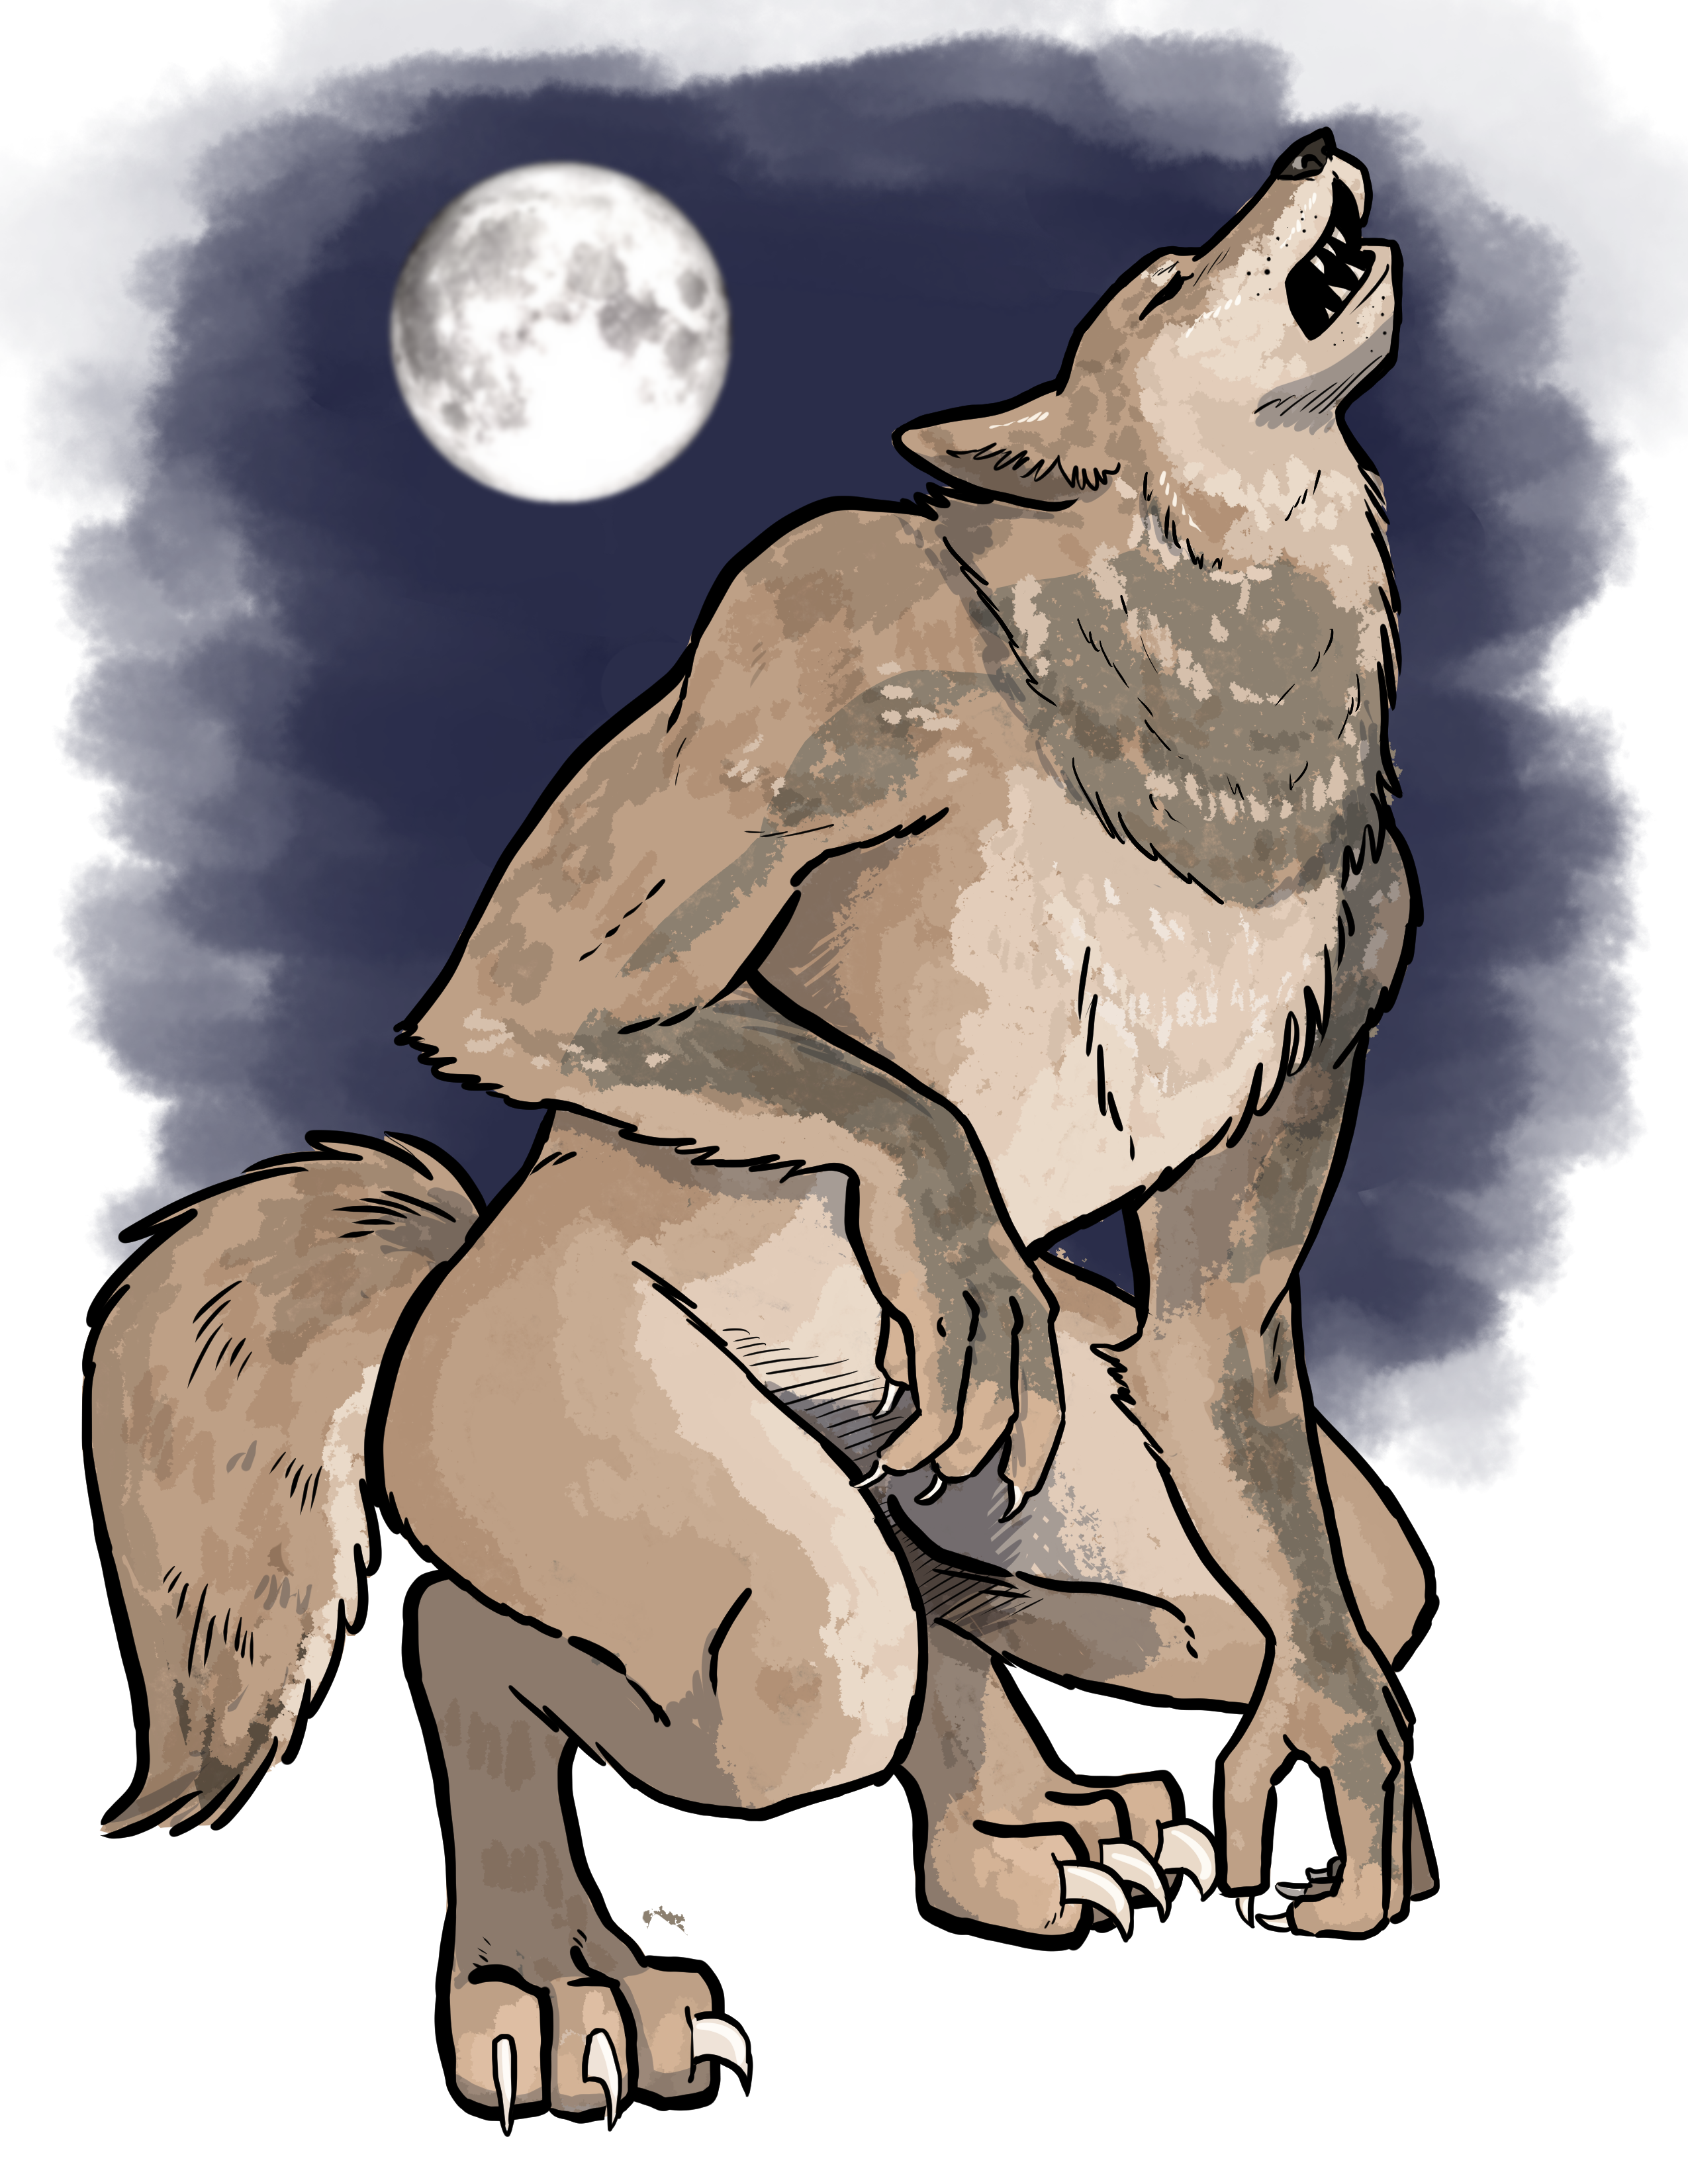
\includegraphics[width=\columnwidth]{Monsters/Lycanthrope, Werewolf}

\subsection{Manta Ray}\index[monsters]{Manta Ray}
\statblock{\textbf{Size:} Large

\textbf{Type:} Animal

\textbf{Habitat:} Ocean (Common)

\textbf{Wandering Group:} 0 (Nil)

\textbf{Lair Group:} 1d3 (Nil)

\textbf{Move:} 40 ft. (Swim)

\textbf{Armor Class:} 6

\textbf{Hit Dice:} 4* (18 HP)

\textbf{Attacks:} Tail (1d8)

\textbf{Special:} Poison

\textbf{Save:} F2

\textbf{Alignment:} None

\textbf{Intelligence:} 2

\textbf{Morale:} 7

\textbf{XP Value:} 125}

Manta rays are flat fish that are related to sharks. Their bodies are shaped with distinctive “wings”, with which they glide along the sea bed.

When a manta ray settles, it covers itself in sand until it is completely invisible.

A manta ray will normally eat only small fish, and ignore large targets. However, if trodden on, a manta ray will attack with the poisonous sting on its tail.

\textbf{Poison:} Anyone struck by the tail of a manta ray must make a saving throw vs. paralysis or be paralyzed for 2d4x10 minutes.

\subsection{Manticore}\index[monsters]{Manticore}
\statblock{\textbf{Size:} Large

\textbf{Type:} Monster

\textbf{Habitat:} Mountains (Rare)

\textbf{Wandering Group:} 1d2 (Nil)

\textbf{Lair Group:} 1d4 (F)

\textbf{Move:} 40 ft., 60 ft. (Fly)

\textbf{Armor Class:} 4

\textbf{Hit Dice:} 6+1* (28 HP)

\textbf{Attacks:} 2x Claw (1d4) \& Bite (2d4) or Special

\textbf{Special:} Spike Shot

\textbf{Save:} F6

\textbf{Alignment:} None

\textbf{Intelligence:} 3

\textbf{Morale:} 9

\textbf{XP Value:} 650}

A manticore is a strange creature with the body of a lion, the wings of a bat, a human face, and a spike covered tail. Despite the human seeming face, manticores are not sapient.

Manticores are aggressive hunters, and will attempt to kill and eat even well armed groups of travelers.

\textbf{Spike Shot:} A manticore has 24 tail spikes, and can shoot six of them per round (range: 50/100/150), even when it is flying. Spikes are re-grown at a rate of two per day.

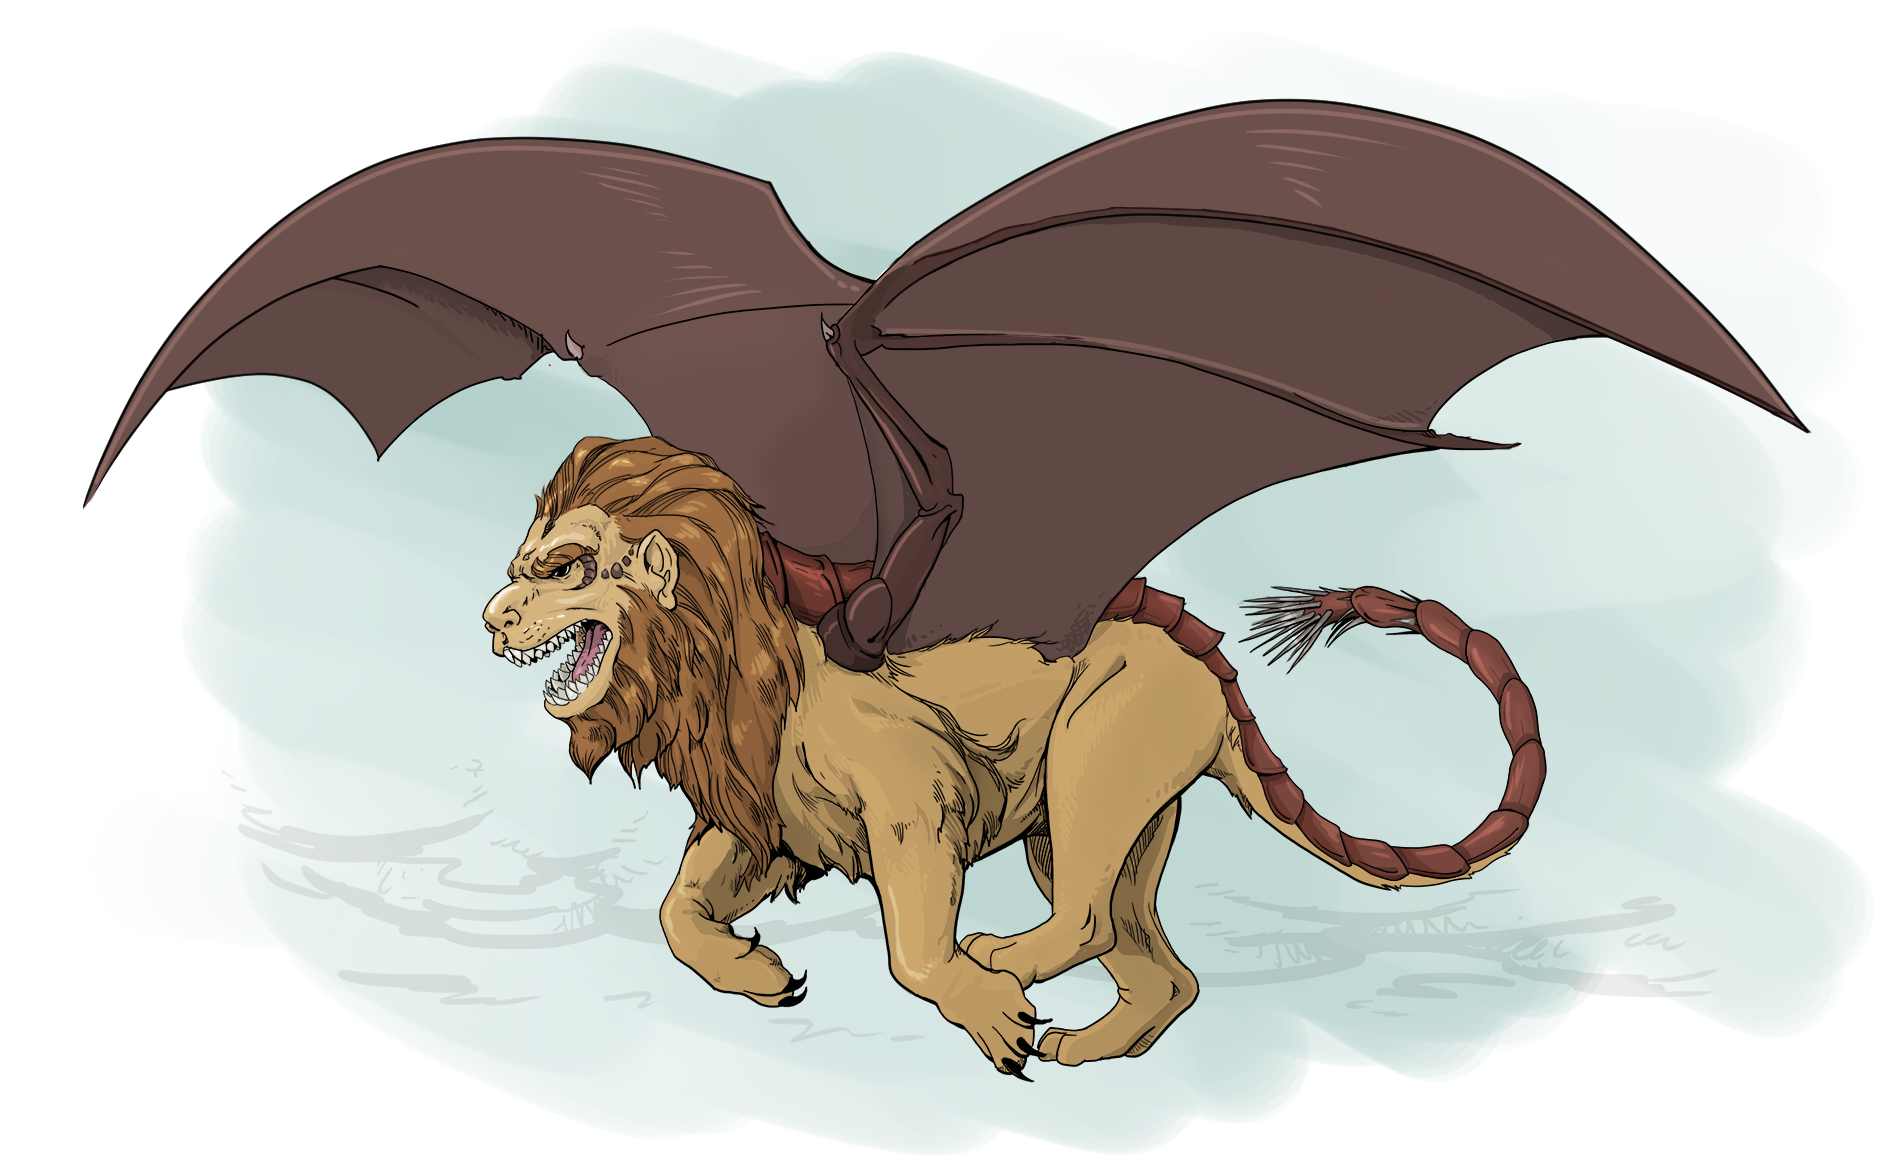
\includegraphics[width=\columnwidth]{Monsters/Manticore}

\subsection{Medusa}\index[monsters]{Medusa}
\begin {table}[H]
	\normalsize
  \begin{tabularx}{\columnwidth}{>{\bfseries}XXX}
	\hiderowcolors
	& \textbf{Prime Plane} & \textbf{Home Plane}\\
	Size: & Medium & Medium\\
	Type: & Extraplanar, & Monster\\
	& Humanoid\\
	Habitat: & Any (Rare) & Elemental Plane of Earth (Very Rare)\\
	Wandering Group: & 1d3 (V) & 1d3 (V)\\
	Lair Group: & 1d4 (F) & 1d4 (F)\\
	Move: & 30 ft. & 60 ft.\\
	Armor Class: & 8 & 4\\
	Hit Dice: & 4** (18 HP) & 8** (36 HP)\\
	Attacks: & Snakebite (1d4) & 10x Tentacle\\
	Special: & Petrifying Gaze, Poison & Paralyzing Grab\\
	Save: & F4 (see below) & F4\\
	Alignment: & Chaotic & Chaotic\\
	Intelligence: & 9 & 9\\
	Morale: & 8 & 9\\
	XP Value: & 175 & 1,750\\
	\showrowcolors
  \end {tabularx}
\end {table}

A medusa appears to be a human with snakes instead of hair. Male medusae are rarely seen, and many people mistakenly think that the race is entirely female. Although the faces of medusae are normally beautiful, their beauty is deceptive and their gaze can turn people to stone.

Although medusae are feared by other races for their gaze, the personalities of individual medusae are as varied as those of humans, although they do have a tendency to be loners and to value their privacy greatly.

\textbf{Petrifying Gaze:} The gaze of a medusa can turn people into stone, but must be direct. Seeing its reflection is not enough to have a chance of being turned to stone. However, a medusa is not immune to its own gaze attack (although it is immune to the gaze of other medusae), and if presented with a mirror, there is a 1 in 6 chance per round that it will see its reflection and must make the saving throw to avoid petrifying itself. This is the only circumstance in which its gaze is effective through a mirror.

Any character surprised by a medusa automatically meets its gaze and must make the saving throw, and in combat each character attacking the medusa without actively avoiding the gaze must also make the saving throw each round.

Characters trying to fight the medusa blindfolded or otherwise averting their gaze will not be affected but must attack with a -4 penalty to hit and the medusa gets a +2 bonus against characters using such tactics.

A character using a mirror to attack in melee (the mirror takes one hand, so the character cannot use an off-hand weapon or a shield at the same time) takes only a -2 penalty to hit and the medusa gets no bonus against them.

\textbf{Poison:} The bite of a medusa’s snakes is poisonous, and anyone bitten must make a saving throw vs. poison or die. Additionally, any creature meeting its gaze must make a saving throw vs. petrification or be turned to stone.

\subsubsection{Home Plane}
Medusae originate from the Elemental Plane of Earth. When on that plane they appear as a hideous mass of 10-foot long tentacles protruding from a small lumpy spherical body. Their are several foot-long eyestalks connected to the body and the mouth has many teeth.

\textbf{Paralyzing Grab:} With a successful tentacle attack, the victim must save vs. paralyzation or become paralyzed for 2d4 rounds. Paralyzed victims are drawn to the medusa's mouth and are automatically bitten for 2d8 points of damage per round.

\subsubsection{Spellcasting}
Medusae can be shamans (to \nth{8} level) or sorcerers (to \nth{8} level).

\subsection{Merfolk}\index[monsters]{Merfolk}
\monsterimage{Monsters/Merfolk}{\statblock{\textbf{Size:} Medium

\textbf{Type:} Humanoid

\textbf{Habitat:} Ocean (Common)

\textbf{Wandering Group:} 0 (Nil)

\textbf{Lair Group:} 1d20 (A)

\textbf{Move:} 40 ft.

\textbf{Armor Class:} 6

\textbf{Hit Dice:} 1 (5 HP)

\textbf{Attacks:} Weapon (By weapon)

\textbf{Special:} None

\textbf{Save:} F1

\textbf{Alignment:} Neutral

\textbf{Intelligence:} 12

\textbf{Morale:} 8

\textbf{XP Value:} 10}}

Merfolk are water breathing humanoids with a fish-like tail instead of legs. Merfolk can only stay out of water as long as they can hold their breaths—which is just like a normal human holding their breath.

Merfolk society is similar to human society. They live in underwater cities and keep domesticated animals.

Merfolk communities often trade with land based creatures, and are usually on good terms with human countries.

\textbf{Dolphin Song:} Merfolk can communicate with dolphins and whales within 500 feet by singing their language. They may also use this song to communicate with other merfolk.

\subsubsection{Spellcasting}
In theory, any merfolk can be a shaman (to \nth{8} level) or sorcerer (to \nth{8} level), although their society teaches that shamanism is an exclusively male role and sorcery is an exclusively female role. Consequently, most human contact is with mermaid sorcerers capable of casting Water Breathing (which allows them to breathe air).

\subsubsection{As a Class}\index[classes]{Merfolk}
Merfolk can be used as a class using the following statistics:

\statblock{\textbf{Ability Requirements:} None

\textbf{Prime Requisite:} Strength, Dexterity, Intelligence, or Wisdom

\textbf{Ability Modifiers:} Dexterity +1, Intelligence -1

\textbf{Weapons:} Any

\textbf{Armor:} None

\textbf{Natural AC:} 7

\textbf{Special Abilities:} Dolphin Song

\textbf{Magic Item Use:} Fighter}

\begin {table}[H]
  \caption{Merfolk Progression}
  \begin{tabularx}{\columnwidth}{>{\bfseries}YYY}
  \thead{Level} & \thead{Experience} & \thead{Hit Dice}\\
	0 & 0 & 1d8\\
	1 & 1,000 & 2d8\\
	2 & 2,000 & 3d8\\
	3 & 4,000 & -\\
	4 & 8,000 & 4d8\\
	5 & 16,000 & 5d8\\
	6 & 32,000 & 6d8\\
	7 & 64,000 & -\\
	8 & 130,000 & 7d8\\
	9 & 260,000 & +2 HP\\
	10+ & +200,000 & +2 HP
  \end {tabularx}
\end {table}

\subsection{Minotaur}\index[monsters]{Minotaur}
\monsterimage{Monsters/Minotaur}{\statblock{\textbf{Size:} Large

\textbf{Type:} Humanoid

\textbf{Habitat:} Underground (Common)

\textbf{Wandering Group:} 1d6 (Nil)

\textbf{Lair Group:} 1d8 (C)

\textbf{Move:} 40 ft.

\textbf{Armor Class:} 6

\textbf{Hit Dice:} 6* (27 HP)

\textbf{Attacks:} Gore (1d6) \& Bite (1d6) 

or Weapon (By weapon + 2)

\textbf{Special:} Wayfinding

\textbf{Save:} F6

\textbf{Alignment:} Chaotic

\textbf{Intelligence:} 5

\textbf{Morale:} 12

\textbf{XP Value:} 500}}

Minotaurs are humanoids with the heads of bulls. They are incredibly aggressive and will attack most other creatures on sight in an attempt to kill and eat them.

Minotaurs love to live and hunt in maze-like tunnel systems and are expert at both finding their way through mazes and tracking. 

\textbf{Wayfinding:} Because of their familiarity with labyrinths, minotaurs are treated as if having 18 intelligence for purposes of the Maze spell.

\subsubsection{Spellcasting}
Although barely sapient, some of the calmer and more level-headed minotaurs can become shamans (to level 4) or even sorcerers (to level 2).

\subsubsection{As a Class}\index[classes]{Minotaur}
Minotaurs can be used as a class using the following statistics:

\statblock{\textbf{Ability Requirements:} Strength 12, Dexterity 5, Constitution 12, Intelligence 5

\textbf{Prime Requisite:} Strength and Constitution

\textbf{Ability Modifiers:} Strength +2, Constitution +2, Wisdom -2, Charisma -2

\textbf{Weapons:} Any

\textbf{Armor:} Any

\textbf{Natural AC:} 5

\textbf{Special Abilities:} Wayfinding

\textbf{Magic Item Use:} Fighter}

\begin {table}[H]
  \caption{Minotaur Progression}
  \begin{tabularx}{\columnwidth}{>{\bfseries}YYY}
  \thead{Level} & \thead{Experience} & \thead{Hit Dice}\\
	1 & 0 & 1d8+6\\
	2 & 3,780 & 2d8\\
	3 & 7,560 & 3d8\\
	4 & 15,120 & 4d8\\
	5 & 30,240 & 5d8\\
	6 & 60,480 & 6d8\\
	7 & 120,960 & 7d8\\
	8 & 236,250 & 8d8\\
	9 & 472,500 & +2 HP\\
	10 & 708,750 & +2 HP\\
	11+ & +240,000 & +2 HP
  \end {tabularx}
\end {table}

\subsection{Mujina}\index[monsters]{Mujina}
\statblock{\textbf{Size:} Medium

\textbf{Type:} Monster

\textbf{Habitat:} Any (Very Rare)

\textbf{Wandering Group:} 1d4 (Nil)

\textbf{Lair Group:} 1d4 (E)

\textbf{Move:} 40 ft.

\textbf{Armor Class:} 4

\textbf{Hit Dice:} 8** (36 HP)

\textbf{Attacks:} 2x Weapon (By weapon)

\textbf{Special:} Change Face, Dual Wield

\textbf{Save:} F8

\textbf{Alignment:} Chaotic

\textbf{Intelligence:} 10

\textbf{Morale:} 9

\textbf{XP Value:} 1,750}

Mujina are a strange humanoid race. They appear similar to humans, except that they have no features on their heads. Their heads are just smooth ovals.

Mujina all have absolutely identical personalities, and no sense of individualism. They hate all creatures that show diversity of personality; especially humans, who show the most diversity of all races.

\textbf{Change Face:} Mujina can mask their head an in illusion that makes it look like whatever they like, including a copy of someone else’s face.

A mujina can drop its illusion at any time, and anyone seeing the true blankness of the mujina’s face must run in terror for 1d3 rounds. Creatures with 5 or more hit dice may make a saving throw vs. wands to avoid this effect.

\textbf{Duel Wield:} Mujina are incredibly strong, and can wield a two handed weapon in either hand without penalty.

\subsection{Mule}\index[monsters]{Mule}
\statblock{\textbf{Size:} Large

\textbf{Type:} Animal

\textbf{Habitat:} Any (Common)

\textbf{Wandering Group:} 0 (Nil)

\textbf{Lair Group:} 2d12 (Nil)

\textbf{Move:} 40 ft.

\textbf{Armor Class:} 7

\textbf{Hit Dice:} 2 (9 HP)

\textbf{Attacks:} Kick (1d4)

\textbf{Special:} None

\textbf{Save:} F0

\textbf{Alignment:} None

\textbf{Intelligence:} 2

\textbf{Morale:} 8

\textbf{XP Value:} 20}

Mules are domestic cross-breeds between donkeys and horses.

They are commonly used as pack animals, since they combine the strength of a horse with the stamina and patience of a donkey.

Mules will allow themselves to be led into underground areas.

\subsection{Mummy}\index[monsters]{Mummy}
\monsterimage[-.2]{Monsters/Mummy}{\statblock{\textbf{Size:} Medium

\textbf{Type:} Undead

\textbf{Habitat:} Desert, Underground (Rare)

\textbf{Wandering Group:} 1d4 (Nil)

\textbf{Lair Group:} 1d12 (D)

\textbf{Move:} 20 ft.

\textbf{Armor Class:} 3*

\textbf{Hit Dice:} 5+1** (24 HP)

\textbf{Attacks:} Touch (1d12)

\textbf{Special:} Despair, Immunity 

(Mind Effects, Normal Weapons, 

Poison), Mummy Rot, 

Resistance to Non-Fire Damage

\textbf{Save:} F5

\textbf{Alignment:} Chaotic

\textbf{Intelligence:} 6

\textbf{Morale:} 12

\textbf{XP Value:} 575}}

Mummies are re-animated corpses that have been specially prepared and wrapped so that they will become undead.

Mummies are normally placed as tomb guardians, but occasionally one or more will wander from its tomb and wreak havoc—especially if the tomb has already been looted.

\textbf{Despair:} Anyone seeing a mummy must make a saving throw vs. paralysis or be paralyzed in fear until the mummy is no longer in sight.

\textbf{Mummy Rot:} Anyone touched by a mummy contracts mummy rot (no saving throw). Mummy rot prevents its victim from being healed by mortal level magic, and makes all natural healing take ten times as long as normal to occur. It can be cured by a Cure Disease effect.

\textbf{Resistance to Non-Fire Damage:} Attacks from sources other than fire only do half damage to mummies.

\subsection{Neanderthal}\index[monsters]{Neanderthal}\label{monster:Neanderthal}
\statblock{\textbf{Size:} Medium

\textbf{Type:} Humanoid

\textbf{Habitat:} Any (Rare)

\textbf{Wandering Group:} 1d10 (Nil)

\textbf{Lair Group:} 4d10 (C)

\textbf{Move:} 40 ft.

\textbf{Armor Class:} 8

\textbf{Hit Dice:} 2 (9 HP)

\textbf{Attacks:} Weapon (By weapon + 1)

\textbf{Special:} Craft (Leatherworking and Masonry)

\textbf{Save:} F2

\textbf{Alignment:} Lawful

\textbf{Intelligence:} 7

\textbf{Morale:} 7

\textbf{XP Value:} 20}

Neanderthals are closely related to humans, although they are squat and ape-like, with sloping brows.

They mostly live in hilly or mountainous regions, where they have a peaceful hunter gatherer existence.

\textbf{Craft (Leatherworking and Masonry):} Although they haven't developed cooking and metalworking skills, neanderthals are experts at making weapons and tools from hides or stone such as flint.

Neanderthals often keep cave apes or dire wolves as pets.

\subsubsection{Spellcasting}
Neanderthals can be shamans (to \nth{4} level) or sorcerers (to \nth{2} level).

\subsubsection{As a Class}\index[classes]{Neanderthal}
Neanderthals can be used as a class using the following statistics:

\textbf{Determine Depth and Direction:} While underground, neanderthals have a 2 in 6 (1-2 on 1d6) chance of sensing direction or noticing if passages are sloped. Neanderthals must be actively searching for these abilities to function.

\statblock{\textbf{Ability Requirements:} Strength 10, Constitution 9

\textbf{Prime Requisite:} Strength

\textbf{Ability Modifiers:} None

\textbf{Weapons:} Any

\textbf{Armor:} Any

\textbf{Special Abilities:} Determine Depth and Direction

\textbf{Required Skills:} Craft (Leatherworking), Craft (Masonry)

\textbf{Magic Item Use:} Fighter}

\begin {table}[H]
  \caption{Neanderthal Progression}
  \begin{tabularx}{\columnwidth}{>{\bfseries}YYY}
  \thead{Level} & \thead{Experience} & \thead{Hit Dice}\\
	1 & 0 & 1d6\\
	2 & 4,001 & 2d6\\
	3 & 8,001 & 3d6\\
	4 & 16,001 & 4d6\\
	5 & 32,001 & 5d6\\
	6 & 64,001 & 6d6\\
	7 & 120,001 & 6d6+3\\
	8 & 240,001 & 6d6+6\\
	9 & 480,001 & 6d6+9\\
	10+ & +120,000 & +3 HP
  \end {tabularx}
\end {table}

\subsection{Nightshade}
Nightshades are extremely intelligent and incredibly powerful undead. Because they know that they are so conspicuous that operating openly would attract the attention of all the most powerful foes, they usually remain hidden and work through their minions as an Undead Liege. Nightshades desire to completely eradicate the living and make everyone undead, and work towards that end, although they do not co-operate well with others in anything other than a relationship of absolute dominance.

Nightshades are only hit by +3 weapons or better.

\textbf{Aura of Spoilage:} Nightshades emanate a distinctive chilling aura within 120 feet which spoils all consumables (no save), including food, potions, and even holy water. Spoiled consumables are not poisonous, but are inedible and useless. This aura usually prevents the nightshade from surprising opponents.

\textbf{Poison:} Any creature touching a nightshade must make a saving throw vs. poison or die. This poison does not travel through weapons, so melee attacks with weapons are safe.

\textbf{Resistance to Breath Weapons:} Nightshades take only half damage from breath weapons.

\textbf{Resistance to Turning:} Nightshades are resistant to being Turned, and may make a saving throw vs. spells to ignore an attempt to turn them. If the turn result is a ‘D’, then they may make a second saving throw to reduce it to a ‘T’.

\textbf{Spell-like Abilities:} Nightshades can cast the following spells, as if \nth{21} level casters: \iref[spell:Detect Magic]{Detect Magic} (constant), \iref[spell:Detect Invisible]{Detect Invisible} (constant), \ilink{spell:Cause Disease}{Cause Disease} (at will), \iref[spell:Charm Person]{Charm Person} (at will), \iref[spell:Cloudkill]{Cloudkill} (at will), \iref[spell:Confusion]{Confusion} (at will), \ilink{spell:Darkness}{Darkness} (at will), \iref[spell:Dispel Magic]{Dispel Magic} (at will), \ilink{spell:Finger of Death}{Finger of Death} (at will), \iref[spell:Haste]{Haste} (at will), \iref[spell:Hold Person]{Hold Person} (at will), and \iref[spell:Invisibility]{Invisibility} (at will).

\subsubsection{Nightcrawler}\index[monsters]{Nightcrawler}
\statblock{\textbf{Size:} Large

\textbf{Type:} Undead

\textbf{Habitat:} Any (Very Rare)

\textbf{Wandering Group:} 1 (Nil)

\textbf{Lair Group:} 1 (Nil)

\textbf{Move:} 40 ft.

\textbf{Armor Class:} -4*

\textbf{Hit Dice:} 27***** (122 HP)

\textbf{Attacks:} Bite (2d10) \& Sting (2d4)

\textbf{Special:} Aura of Spoilage, Immunity (Cold, Illusions, 

Mind Effects, Petrification, Poison, Spells < \nth{6} level, Wands), 

Poison, Resistance to Breath Weapons, 

Resistance to Turning, Shrinking Gaze, Swallow Whole

\textbf{Save:} F27 (see below)

\textbf{Alignment:} Chaotic

\textbf{Intelligence:} 19

\textbf{Morale:} 12

\textbf{XP Value:} 21,500}

Nightcrawlers appear to be rotting maggots or worms that can burrow through the earth. 

\textbf{Poison:} Anyone bitten or stung by a nightcrawler must make a saving throw vs. poison or die.

When stung, even if the saving throw is successful, there is a 1 in 8 chance that the poison will kill the victim anyway.

\textbf{Shrinking Gaze:} A nightcrawler has a gaze attack that it can use instead of physically attacking or casting spells, that will magically shrink one opponent per round within 60 feet down to 1 foot in height unless that opponent can make a saving throw vs. spells. The nightcrawler gains a +4 bonus to hit that opponent, and can swallow it on a 15-20 rather than just a 19-20.

The shrinking effect is permanent until dispelled.

\textbf{Swallow Whole:} If a nightcrawler bites an opponent of human size or less with a natural roll of 19-20, the opponent is swallowed. Swallowed victims lose one level per round due to an \iref[sec:Energy Drain]{Energy Drain} unless protected by a \iref[spell:Protection from Evil]{Protection from Evil} spell.

\subsubsection{Nightwalker}\index[monsters]{Nightwalker}
\statblock{\textbf{Size:} Large

\textbf{Type:} Undead

\textbf{Habitat:} Any (Very Rare)

\textbf{Wandering Group:} 1 (Nil)

\textbf{Lair Group:} 1 (Nil)

\textbf{Move:} 50 ft., 20 ft. (Fly)

\textbf{Armor Class:} -6*

\textbf{Hit Dice:} 23***** (104 HP)

\textbf{Attacks:} 2x Bash (3d10)

\textbf{Special:} Aura of Spoilage, Cursing Gaze, Immunity (Cold, Illusions, 

Mind Effects, Petrification, Poison, Spells < \nth{6} level, Wands), 

Poison, Resistance to Breath Weapons, 

Resistance to Turning, Spell-like Abilities

\textbf{Save:} F23 (see below)

\textbf{Alignment:} Chaotic

\textbf{Intelligence:} 19

\textbf{Morale:} 12

\textbf{XP Value:} 15,500}

Nightwalkers appear to be rotting giants who never wear clothes or carry items.

\textbf{Cursing Gaze:} A nightwalker has a gaze attack that it can use instead of physically attacking or casting spells, that will magically curse one opponent per round within 60 feet unless that opponent can make a saving throw vs. spells. A cursed character takes a -4 penalty on all attack rolls and saving throws, until the curse is removed by either a Dispel Evil cast by anyone or a Remove Curse cast by a spellcaster of at least \nth{25} level.

\textbf{Destroy Armor:} The nightwalker's blows are so powerful that they have a 50\% chance of destroying their foe’s armor or shield. This chance is reduced by 10\% per magical “plus” of the item. Check for armor being destroyed only if the foe is not using a shield.

\subsubsection{Nightwing}\index[monsters]{Nightwing}
\statblock{\textbf{Size:} Large

\textbf{Type:} Undead

\textbf{Habitat:} Any (Very Rare)

\textbf{Wandering Group:} 1 (Nil)

\textbf{Lair Group:} 1 (Nil)

\textbf{Move:} 10 ft., 80 ft. (Fly)

\textbf{Armor Class:} -8*

\textbf{Hit Dice:} 19***** (104 HP)

\textbf{Attacks:} Bite (1d6+6)

\textbf{Special:} Aura of Spoilage, Cursing Gaze, Immunity (Cold, Illusions, 

Mind Effects, Petrification, Poison, Spells < \nth{6} level, Wands), 

Poison, Resistance to Breath Weapons, 

Resistance to Turning, Spell-like Abilities

\textbf{Save:} F19 (see below)

\textbf{Alignment:} Chaotic

\textbf{Intelligence:} 19

\textbf{Morale:} 12

\textbf{XP Value:} 10,000}

Nightwings appear to be giant rotting bats.

\textbf{Cursing Gaze:} A nightwing has a gaze attack that it can use instead of physically attacking or casting spells, that will magically curse one opponent’s weapon, shield or armor per round within 60 feet unless that opponent can make a saving throw vs. spells. A cursed item temporarily loses one point of magical “plus”, until the curse is removed by either a Dispel Evil cast by anyone or a Remove Curse cast by a spellcaster of at least \nth{25} level.

\textbf{Poison:} Anyone bitten by a nightwing must make a saving throw vs. poison or die. If the victim survives, they must also make a saving throw vs. spells or be polymorphed into a giant bat. Any opponent turned into a bat becomes a loyal servant of the nightwing until the polymorph is dispelled.

\subsection{Nixie}\index[monsters]{Nixie}
\statblock{\textbf{Size:} Small

\textbf{Type:} Humanoid

\textbf{Habitat:} River (Rare)

\textbf{Wandering Group:} 0 (Nil)

\textbf{Lair Group:} 2d20 (B)

\textbf{Move:} 40 ft.

\textbf{Armor Class:} 7

\textbf{Hit Dice:} 1* (5 HP)

\textbf{Attacks:} Miniature Trident (1d6) or Special

\textbf{Special:} Charm Person

\textbf{Save:} E1

\textbf{Alignment:} Neutral

\textbf{Intelligence:} 13

\textbf{Morale:} 6

\textbf{XP Value:} 13}

Nixies are water spirits that take the appearance of small human women. They are bound to their river or lake in the same way that dryads are bound to their tree, and can only survive for 10 minutes if taken more than 240 feet away from their water.

\textbf{Charm Person:} Ten nixies working together can cast a Charm Person spell, and they will often use this to persuade intruders to stay with them as companions. The victim is allowed a save vs. spells to avoid the effect. If they fail they must stay with the nixies for or a year or until the nixie releases the charm

Nixies can each cast Water Breathing once per day, and this lasts for 24 hours.

\subsubsection{Spellcasting}
Occasionally, nixies can be shamans (to \nth{6} level) or sorcerers (to \nth{4} level).

\subsubsection{As a Class}\index[classes]{Nixie}
Nixies can be used as a class using the following statistics:

\textbf{Charm Person:} For every level beyond 0 that a nixie reaches, they count as an extra nixie for the purpose of charming a person.

\statblock{\textbf{Ability Requirements:} None

\textbf{Prime Requisite:} Strength, Dexterity, Intelligence, or Wisdom

\textbf{Ability Modifiers:} Strength -2, Dexterity -1, Charisma -1

\textbf{Weapons:} Daggers, Miniature Trident

\textbf{Armor:} None

\textbf{Natural AC:} 7

\textbf{Special Abilities:} Charm Person

\textbf{Magic Item Use:} Fighter}

\begin {table}[H]
  \caption{Nixie Progression}
  \begin{tabularx}{\columnwidth}{>{\bfseries}YYY}
  \thead{Level} & \thead{Experience} & \thead{Hit Dice}\\
	0 & 0 & 1d8\\
	1 & 1,800 & 3d8\\
	2 & 3,600 & 3d8\\
	3 & 7,200 & 3d8\\
	4 & 14,400 & 4d8\\
	5 & 28,800 & 5d8\\
	6 & 60,000 & 6d8\\
	7 & 120,000 & 6d8\\
	8 & 240,000 & 7d8\\
	9 & 480,000 & 7d8+2\\
	10+ & +300,000 & +2 HP
  \end {tabularx}
\end {table}

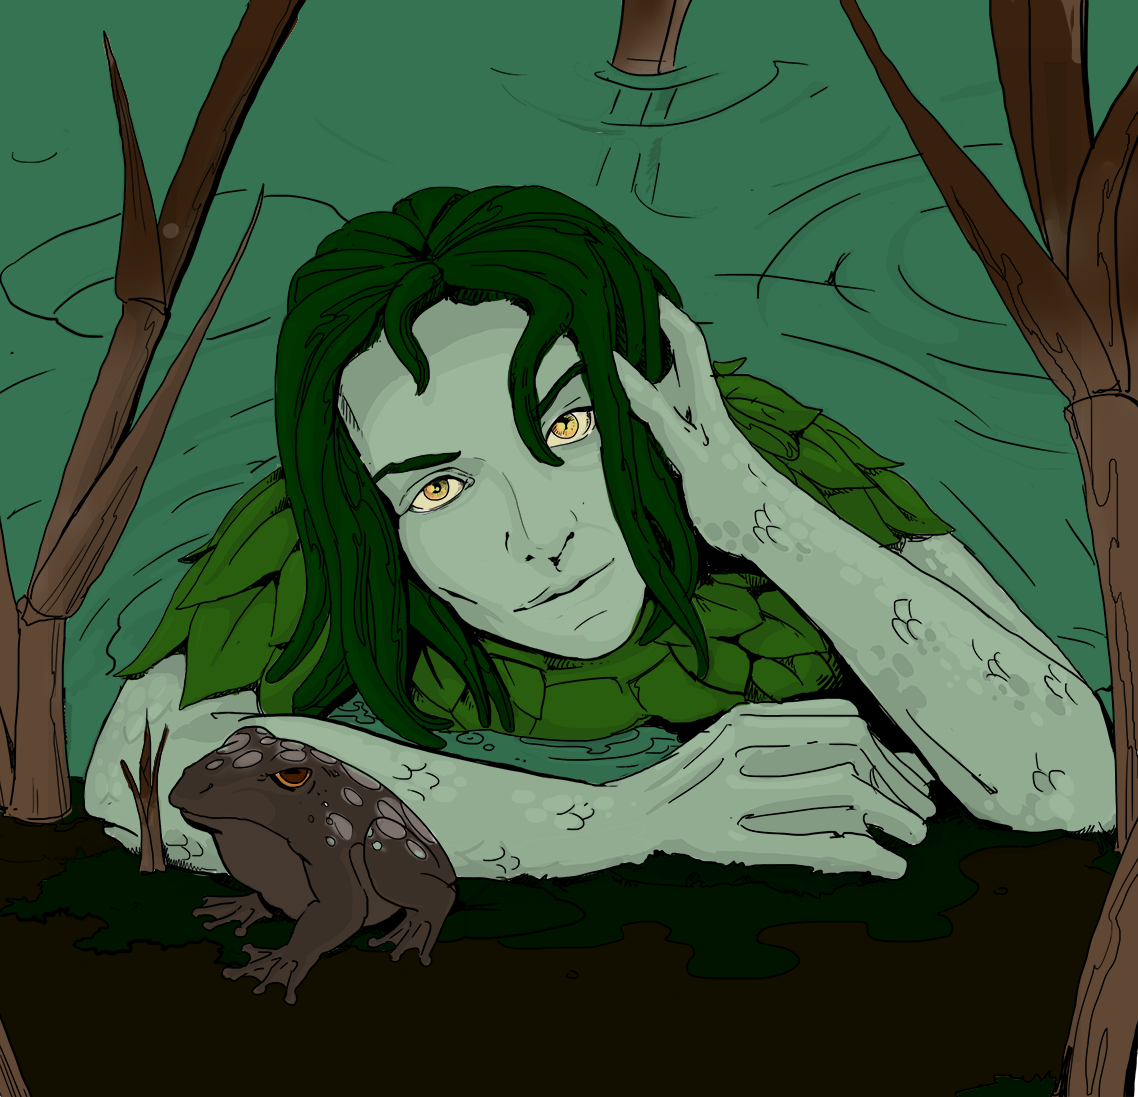
\includegraphics[width=\columnwidth]{Monsters/Nixie}

\subsection{Nuckalavee}\index[monsters]{Nuckalavee}
\statblock{\textbf{Size:} Large

\textbf{Type:} Monster

\textbf{Habitat:} Ocean (Rare)

\textbf{Wandering Group:} 0 (Nil)

\textbf{Lair Group:} 1 (Nil)

\textbf{Move:} 40 ft., 120 ft. (Swim)

\textbf{Armor Class:} 4*

\textbf{Hit Dice:} 11*** (50 HP)

\textbf{Attacks:} 2x Claw (3d8)

\textbf{Special:} Aura of Death/Fear, Cone of Cold, 

Death Touch, Immunity (Fire, Poison), Regeneration (3)

\textbf{Save:} F11

\textbf{Alignment:} Chaotic

\textbf{Intelligence:} 9

\textbf{Morale:} 10

\textbf{XP Value:} 3,500}

A nuckalavee appears similar to a centaur with transparent skin, so that all the muscles and organs can be seen. Nuckalavees are amphibious, and live in coastal waters.

Although not undead themselves, nuckalavee are friendly with undead creatures and can act as an Undead Liege.

\textbf{Aura of Death/Fear:} A nuckalavee has an aura with a 120-foot range that kills all small insects, birds, rodents, and other similar creatures with 2 hit points or less. Within 50 feet all creatures must make a saving throw vs. paralysis or flee in terror for 2d6 rounds. This saving throw must be made each round.

\textbf{Cone of Cold:} A nuckalavee can breathe a cone of cold 60 feet long and 10 feet wide at the end that does damage equal to its current hit points (save vs. breath weapons for half damage).

\textbf{Death Touch:} Anyone struck by a nuckalavee must make a saving throw vs. death ray or die.

\subsubsection{Spellcasting}
Nuckalavee can be shamans (to \nth{2} level) or sorcerers (to \nth{4} level).

\subsection{Ochre Jelly}\index[monsters]{Ochre Jelly}
\statblock{\textbf{Size:} Large

\textbf{Type:} Ooze

\textbf{Habitat:} Underground (Common)

\textbf{Wandering Group:} 1 (Nil)

\textbf{Lair Group:} 0 (Nil)

\textbf{Move:} 10 ft.

\textbf{Armor Class:} 8

\textbf{Hit Dice:} 5* (23 HP)

\textbf{Attacks:} Touch (2d6)

\textbf{Special:} Dissolve, Split

\textbf{Save:} F3

\textbf{Alignment:} None

\textbf{Intelligence:} 0

\textbf{Morale:} 12

\textbf{XP Value:} 300}

An ochre jelly is an orange-brown amoeba-like ooze.

Ochre jellies can only be harmed by fire or cold. Other attacks do no damage.

\textbf{Dissolve:} An ochre jelly can dissolve wood, leather or cloth in one turn, but cannot eat through metal.

\textbf{Split:} Psychical attacks will split the ochre jelly into 1d4+1 smaller (2 hit dice, attack bonus +3, 1d6 damage) jellies.

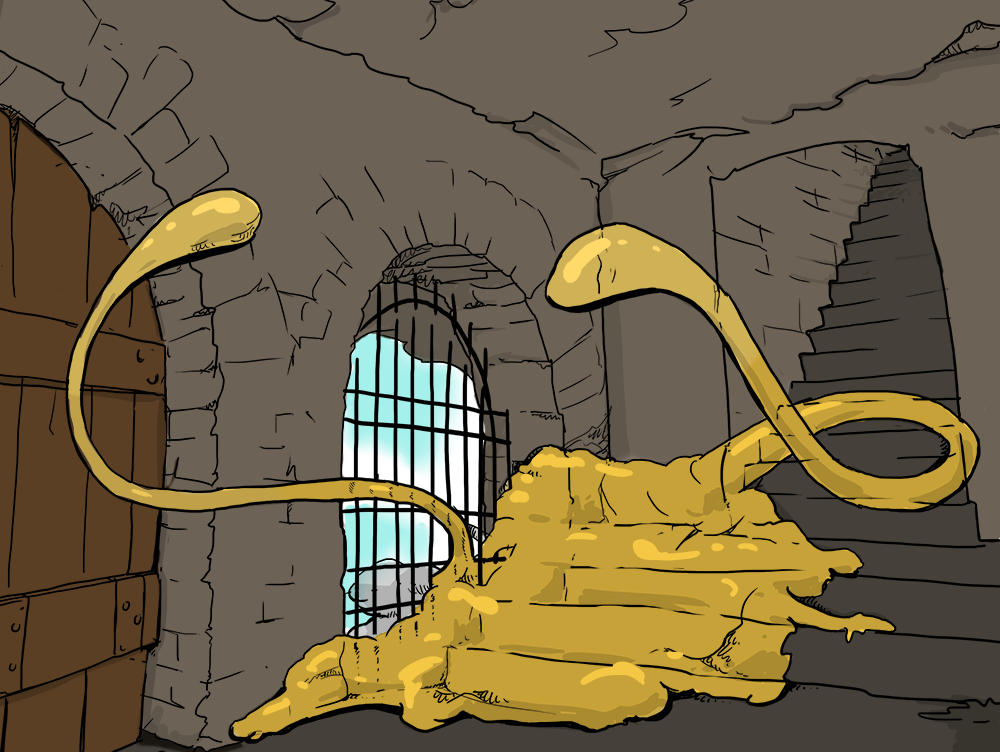
\includegraphics[width=\columnwidth]{Monsters/Ochre Jelly}

\subsection{Ogre}\index[monsters]{Ogre}
\statblock{\textbf{Size:} Large

\textbf{Type:} Humanoid

\textbf{Habitat:} Any (Common)

\textbf{Wandering Group:} 1d6 (Sx10)

\textbf{Lair Group:} 2d6 (Sx100 + C)

\textbf{Move:} 30 ft.

\textbf{Armor Class:} 5

\textbf{Hit Dice:} 4+1 (19 HP)

\textbf{Attacks:} Weapon (By weapon + 2)

\textbf{Special:} None

\textbf{Save:} F4

\textbf{Alignment:} Chaotic

\textbf{Intelligence:} 6

\textbf{Morale:} 10

\textbf{XP Value:} 125}

Ogres are heavily built humanoids. Ogres are rather dull witted, and will usually try to bully others to serve them rather than hunt for themselves. When this does not work, they will often work as hired muscle for other creatures. For an ogre, knowing where the next meal is coming from and having shiny coins to count are life’s greatest luxuries.

Ogres are not particularly evil or malicious, but have no qualms about doing unpleasant or immoral tasks if paid to do so. They simply don’t think about what they are doing.

Ogres can occasionally be found working in human settlements, although their tendency to break things can often mean that they are more trouble than they are worth.

\subsubsection{Spellcasting}
Some particularly bright ogres can be shamans (to \nth{4} level) or sorcerers (to \nth{2} level).

\subsubsection{As a Class}\index[classes]{Ogre}
Ogres can be used as a class using the following statistics:

\statblock{\textbf{Ability Requirements:} Strength 16

\textbf{Prime Requisite:} Strength, Dexterity, Intelligence, or Wisdom

\textbf{Ability Modifiers:} Strength +2, Dexterity -1, Constitution +1, Wisdom -1

\textbf{Weapons:} Any

\textbf{Armor:} Any

\textbf{Natural AC:} 9

\textbf{Special Abilities:} None

\textbf{Magic Item Use:} Fighter}

\begin {table}[H]
  \caption{Ogre Progression}
  \begin{tabularx}{\columnwidth}{>{\bfseries}YYY}
  \thead{Level} & \thead{Experience} & \thead{Hit Dice}\\
	-2 & -4,800 & 2d8+1\\
	-1 & -2,400 & 3d8+1\\
	0 & 0 & 4d8+1\\
	1 & 4,800 & 5d8+2\\
	2 & 14,200 & 6d8+2\\
	3 & 33,200 & -\\
	4 & 71,200 & 7d8+2\\
	5 & 145,200 & 8d8+2\\
	6 & 295,200 & 9d8+3\\
	7 & 595,200 & -\\
	8 & 895,200 & 10d8+3\\
	9+ & +300,000 & +2 HP
  \end {tabularx}
\end {table}

\subsection{Orc}\index[monsters]{Orc}
\statblock{\textbf{Size:} Medium

\textbf{Type:} Humanoid

\textbf{Habitat:} Any (Common)

\textbf{Wandering Group:} 2d4 (P)

\textbf{Lair Group:} 10d6 (D)

\textbf{Move:} 40 ft.

\textbf{Armor Class:} 6

\textbf{Hit Dice:} 1 (5 HP)

\textbf{Attacks:} Weapon (By weapon)

\textbf{Special:} None

\textbf{Save:} F1

\textbf{Alignment:} Chaotic

\textbf{Intelligence:} 7

\textbf{Morale:} 8

\textbf{XP Value:} 10}

Orcs are pig-headed humanoids with pink skin.

They usually live underground and only come out at night, since they take a -1 penalty to attack rolls in strong daylight.

Orcs have strong tribal structures, and tribes often fight each other and raid each other for slaves. It is not unknown for a slave rebellion in an orc community to end up with the previous masters as the new slaves and the previous slaves forming a new tribe. Orcs will also use goblins, kobolds, or even humans as slaves if they can get them.

Despite their loose social structures, orcs are very industrious and can often be found making weapons and armor for other races. Orcish designs emphasize simplicity and efficiency over decoration and art.

Although orcs sometimes trade with humans, relations are always strained because of the orcs’ slaving tendencies.

\subsubsection{Spellcasting}
Orcs can be shamans (to \nth{6} level) or sorcerers (to \nth{4} level).

\subsubsection{As a Class}\index[classes]{Orc}
Orcs can be used as a class using the following statistics:

\statblock{\textbf{Ability Requirements:} None

\textbf{Prime Requisite:} Strength, Dexterity, Intelligence, or Wisdom

\textbf{Ability Modifiers:} Strength +1, Dexterity -1

\textbf{Weapons:} Any

\textbf{Armor:} Any

\textbf{Natural AC:} 8

\textbf{Special Abilities:} None

\textbf{Magic Item Use:} Fighter}

\begin {table}[H]
  \caption{Orc Progression}
  \begin{tabularx}{\columnwidth}{>{\bfseries}YYY}
  \thead{Level} & \thead{Experience} & \thead{Hit Dice}\\
	0 & 0 & 1d8\\
	1 & 1,000 & 2d8\\
	2 & 2,000 & 3d8\\
	3 & 4,000 & -\\
	4 & 8,000 & 4d8\\
	5 & 16,000 & 5d8\\
	6 & 32,000 & 6d8\\
	7 & 64,000 & -\\
	8 & 130,000 & 7d8\\
	9 & 260,000 & +2 HP\\
	10+ & +200,000 & +2 HP
  \end {tabularx}
\end {table}

\subsection{Owlbear}\index[monsters]{Owlbear}
\statblock{\textbf{Size:} Large

\textbf{Type:} Monster

\textbf{Habitat:} Underground, Woods (Common)

\textbf{Wandering Group:} 1d4 (Nil)

\textbf{Lair Group:} 1d4 (C)

\textbf{Move:} 40 ft.

\textbf{Armor Class:} 5

\textbf{Hit Dice:} 5

\textbf{Attacks:} 2x Claw (1d8) \& Bite (1d8)

\textbf{Special:} Squeeze

\textbf{Save:} F3

\textbf{Alignment:} None

\textbf{Intelligence:} 2

\textbf{Morale:} 9

\textbf{XP Value:} 175}

An owlbear is a bear-like creature with the head of an owl.

Owlbears are bad tempered carnivores, and will often attack even when not hungry.

\textbf{Squeeze:} If an owlbear hits the same opponent with both claw attacks, it can squeeze for an additional 2d8 damage.

\subsection{Pegasus}\index[monsters]{Pegasus}\label{monster:Pegasus}
\statblock{\textbf{Size:} Large

\textbf{Type:} Monster

\textbf{Habitat:} Clear, Hills, Mountains (Rare)

\textbf{Wandering Group:} 0 (Nil)

\textbf{Lair Group:} 1d12 (Nil)

\textbf{Move:} 80 ft., 160 ft. (Fly)

\textbf{Armor Class:} 6

\textbf{Hit Dice:} 2+2 (11 HP)

\textbf{Attacks:} 2x Kick (1d6)

\textbf{Special:} None

\textbf{Save:} F2

\textbf{Alignment:} None

\textbf{Intelligence:} 4

\textbf{Morale:} 8

\textbf{XP Value:} 25}

Pegasi are winged horses. They are more intelligent than normal horses (although not sapient) and can not be domesticated, although they may befriend an individual and allow themselves to be ridden by that individual.



\subsection{Phantom}
Phantoms are transparent (but visible) incorporeal undead creatures. They may be found lurking anywhere, but tend to avoid sunlight.

\textbf{Immunity to Normal Weapons:} A phantom can only be hit by magical weapons.

\textbf{Resistance to Turning:} A phantom can resist Turn attempts. If a phantom is turned with anything other than a ‘D’ result, it can make a saving throw vs. spells to reflect the turn back on the cleric, who must then save vs. spells or be paralyzed for 2d6 rounds.

\subsubsection{Apparition}\index[monsters]{Apparition}
\statblock{\textbf{Size:} Medium

\textbf{Type:} Undead

\textbf{Habitat:} Any (Rare)

\textbf{Wandering Group:} 1 (L)

\textbf{Lair Group:} 1 (N, O)

\textbf{Move:} 60 ft.

\textbf{Armor Class:} 0*

\textbf{Hit Dice:} 10*** (45 HP)

\textbf{Attacks:} 2x Claw (1d6+2)

\textbf{Special:} Create Spawn, Despair, 

Immunity (Mind Effects, Normal Weapons, Poison), 

Paralyzing Mist, Resistance to Turning

\textbf{Save:} W10

\textbf{Alignment:} Chaotic

\textbf{Intelligence:} 11

\textbf{Morale:} 10

\textbf{XP Value:} 3,250}

\textbf{Create Spawn:} Any human or demi-human killed by an apparition will fade away and become one in a week (even if raised) unless a Dispel Evil is cast on them.

\textbf{Despair:} Anyone seeing an apparition within 120 feet must run in fear and be unable to approach the apparition any closer than this radius. Creatures with more than 3 hit dice may make a saving throw vs. spells to avoid this effect.

\textbf{Paralyzing Mist:} An apparition can surround itself with a 20-foot radius of swirling mist. All who enter the mist must make a saving throw vs. spells or be paralyzed for 12 rounds. The apparition will usually attack paralyzed targets first, gaining a +4 to hit.

\subsubsection{Shade}\index[monsters]{Shade}
\statblock{\textbf{Size:} Medium

\textbf{Type:} Undead

\textbf{Habitat:} Any (Rare)

\textbf{Wandering Group:} 1 (L, N, V)

\textbf{Lair Group:} 0 (Nil)

\textbf{Move:} 40 ft.

\textbf{Armor Class:} 0*

\textbf{Hit Dice:} 11***

\textbf{Attacks:} Dagger (3d4)

\textbf{Special:} Charge, Despair, Immunity (Mind Effects, 

Normal Weapons, Poison), Resistance to Turning

\textbf{Save:} R11

\textbf{Alignment:} Chaotic

\textbf{Intelligence:} 10

\textbf{Morale:} 9

\textbf{XP Value:} 3,500}

A shade always stays indoors during the day, only venturing outside at night to quickly move from building to building.

A shade normally attacks by charging through a wall or door, surprising its opponents on a 1-5 on a d6.

\textbf{Charge:} A shade can perform the Charge action in combat. If it does so, it does not make a normal dagger attack at the end of the charge, but dashes up to its target’s face screaming. The target must make a saving throw vs. death ray or immediately drop dead from fear.

\textbf{Despair:} Anyone seeing a shade within 120 feet must run in fear and be unable to approach the shade any closer than this radius. Creatures with more than 3 hit dice may make a saving throw vs. spells to avoid this effect.

\subsubsection{Vision}\index[monsters]{Vision}
\statblock{\textbf{Size:} Medium

\textbf{Type:} Undead

\textbf{Habitat:} Any (Rare)

\textbf{Wandering Group:} 1 (Nil)

\textbf{Lair Group:} 1 (L, N, O)

\textbf{Move:} -

\textbf{Armor Class:} 0*

\textbf{Hit Dice:} 12***

\textbf{Attacks:} Special

\textbf{Special:} Despair, Immunity (Mind Effects, 

Normal Weapons, Poison), Resistance to Turning

\textbf{Save:} C12

\textbf{Alignment:} Chaotic

\textbf{Intelligence:} 9

\textbf{Morale:} 12

\textbf{XP Value:} 3,875}

A vision’s body is composed of lost souls of 2d4 humanoid creatures. The creatures appear mangled as if they died in a fierce battle.

If a vision is successfully turned, it disappears for 1d6 hours.

While in combat, each figure will attack independently with melee weapons and are able to move 40 feet per round but unable to leave the area. A vision has a single collective set of hit points, and when these run out all figures are destroyed.

\textbf{Despair:} A vision will cry and howl when met. All within 90 feet who hear this must make a saving throw vs. spells or collapse in despair and spend 1d10+10 rounds curled up and crying for the lost souls.

\subsection{Phoenix}\index[monsters]{Phoenix}
\statblock{\textbf{Size:} Large

\textbf{Type:} Monster

\textbf{Habitat:} Elemental Plane of Fire (Very Rare)

\textbf{Wandering Group:} 0 (Nil)

\textbf{Lair Group:} 1d2 (Vx2)

\textbf{Move:} 50 ft., 150 ft. (Fly)

\textbf{Armor Class:} -2*

\textbf{Hit Dice:} 18***** (81 HP)

\textbf{Attacks:} 2x Claw (2d6) \& Bite (4d6)

\textbf{Special:} Explode, From the Ashes, Halo of Fire, 

Immunity (Charm, Fire, Hold, Weapons < +3)

\textbf{Save:} F20

\textbf{Alignment:} Neutral

\textbf{Intelligence:} 6

\textbf{Morale:} 10

\textbf{XP Value:} 8,875}

A phoenix is a red-orange eagle-like bird surrounded by a halo of fire. Phoenixes are never hostile unless attacked, but will fight to the death to defend themselves.

\textbf{Explode:} When a phoenix is destroyed, it explodes into a 18d6 Fireball with a 20-foot radius. Creatures in the area may save vs. breath weapon to take half damage, but resistances or immunities to fire do not reduce the damage.

\textbf{From the Ashes:} There is no way short of a Wish to keep a phoenix dead permanently. When a phoenix is destroyed and explodes, it will rise from its own ashes one round later and flee from its attackers if possible.

\textbf{Halo of Fire:} All creatures within 20 feet of a phoenix take 6d6 fire damage per round.

\subsection{Pixie}\index[monsters]{Pixie}
\monsterimage{Monsters/Pixie}{\statblock{\textbf{Size:} Small

\textbf{Type:} Humanoid

\textbf{Habitat:} Woods (Rare)

\textbf{Wandering Group:} 2d4 (R+S)

\textbf{Lair Group:} 4d10 (Nil)

\textbf{Move:} 30 ft., 60 ft. (Fly)

\textbf{Armor Class:} 3

\textbf{Hit Dice:} 1*** (5 HP)

\textbf{Attacks:} Dagger (1d4)

\textbf{Special:} Natural Invisibility

\textbf{Save:} E1

\textbf{Alignment:} Neutral

\textbf{Intelligence:} 14

\textbf{Morale:} 7

\textbf{XP Value:} 19}}

Pixies are elf-like creatures with butterfly wings.

Pixies are not strong fliers, and can only fly for half an hour before having to rest.

Pixies are generally on friendly terms with both humans and elves, although they hate orcs and goblins and do their best to drive them from their woods.

\textbf{Natural Invisibility:} Pixies can make themselves visible when they want to.

\subsubsection{Spellcasting}
Pixies can be shamans (to \nth{6} level) or sorcerers (to \nth{4} level).

\subsubsection{As a Class}\index[classes]{Pixie}
Pixies can be used as a class using the following statistics:

\statblock{\textbf{Ability Requirements:} Dexterity 9, Intelligence 8

\textbf{Prime Requisite:} Dexterity

\textbf{Ability Modifiers:} Strength -1, Dexterity +1, Constitution -1, Charisma +1

\textbf{Weapons:} Any small

\textbf{Armor:} Any small

\textbf{Natural AC:} 6

\textbf{Special Abilities:} Natural Invisibility

\textbf{Magic Item Use:} Fighter; Elf and Wizard (Chance of Misuse, see \fullref{tab:Pixie Magic Item Use})}

\begin {table}[H]
  \caption{Pixie Progression}
  \begin{tabularx}{\columnwidth}{>{\bfseries}YYY}
  \thead{Level} & \thead{Experience} & \thead{Hit Dice}\\
	0 & 0 & 1d8\\
	1 & 2,000 & 2d8\\
	2 & 4,000 & 3d8\\
	3 & 8,000 & 4d8\\
	4 & 16,000 & 5d8\\
	5 & 32,000 & 6d8\\
	6 & 64,000 & 7d8\\
	7 & 128,000 & 8d8\\
	8 & 250,000 & 9d8\\
	9 & 500,000 & 10d8\\
	10+ & +300,000 & +1 HP
  \end {tabularx}
\end {table}

\begin {table}[H]
  \caption{Pixie Magic Item Use}\label{tab:Pixie Magic Item Use}
  \begin{tabularx}{\columnwidth}{>{\bfseries}YYYYY}
	\thead{} & \multicolumn{4}{c}{\thead{d\% Result}}\\
	\thead{Level} & \thead{Success} & \thead{Failure} & \thead{Backfire} & \thead{Unexpected}\\
	1 & 01-05 & 06-84 & 85-99 & 00\\
	2 & 01-10 & 11-84 & 85-98 & 99-00\\
	3 & 01-10 & 11-84 & 85-97 & 98-00\\
	4 & 01-15 & 16-84 & 85-96 & 97-00\\
	5 & 01-20 & 21-84 & 85-95 & 96-00\\
	6 & 01-20 & 21-84 & 85-94 & 95-00\\
	7 & 01-25 & 26-84 & 85-93 & 94-00\\
	8 & 01-30 & 31-84 & 85-92 & 93-00\\
	9 & 01-30 & 31-84 & 85-91 & 92-00\\
	10+ & 01-35 & 36-84 & 85-90 & 91-00
  \end {tabularx}
\end {table}

\subsection{Pooka}\index[monsters]{Pooka}
\monsterimage{Monsters/Pooka}{\statblock{\textbf{Size:} By Animal

\textbf{Type:} Fey

\textbf{Habitat:} Any (Very Rare)

\textbf{Wandering Group:} 1 (Nil)

\textbf{Lair Group:} 0 (Nil)

\textbf{Move:} 40 ft.

\textbf{Armor Class:} 4

\textbf{Hit Dice:} 2** (9 HP)

\textbf{Attacks:} As Animal

\textbf{Special:} Invisibility to Mortals

\textbf{Save:} R2

\textbf{Alignment:} Chaotic/Neutral

\textbf{Intelligence:} 11

\textbf{Morale:} 9

\textbf{XP Value:} 25}}

Pooka are solitary animal spirits with extraordinary powers.

Pooka are very fond of mischief, drinking, magic tricks, music, and other forms of entertainment. They have been known to befriend mortals that provide such entertainment.

\textbf{Age Inanimate Object:} Pooka can age inanimate objects at will by touching them. In effect, this will cause wood to rot, metal to rust, food to spoil, and so forth.

\textbf{Invisibility to Mortals:} The invisibility can be to all mortals or just to select individuals.

\subsubsection{As a Class}\index[classes]{Pooka}
Pooka can be used as a class using the following statistics:

\textbf{Control Dreams:} At level 0 and higher, a pooka can control a sleeping target's dreams. Although the victim is not aware that their dreams are being controlled, they are allowed a saving throw vs. spells to avoid the effect.

\textbf{Time Manipulation:} Besides aging inanimate objects, pooka have various other time manipulation abilities that are acquired and improve as they level gains levels.

\textbf{Haste Self:} Starting at \nth{3} level, pooka can move as if they were affected by a Haste spell. This may be done up to ten rounds per day plus two additional rounds per three levels the pooka has attained.

\textbf{Haste/Slow Other:} Starting at \nth{5} level, a pooka can hasten or slow a target as if they were affected by a Haste/Slow spell. This may be done once per day plus an additional time per two levels the pooka has attained.

\textbf{Fast Healing:} Starting at \nth{7} level, a pooka can speed up the healing process of a target by touching them. The pooka may use this ability for a number of rounds equal to the pooka's level times two. For each round this ability is used, the target regains one hit point.

\textbf{Blink:} Starting at \nth{9} level, a pooka can attempt to briefly step outside of time to avoid attacks and spells. With a successful saving throw vs. spells a single attack or spell is completely avoided. In the case of spells, the pooka is still allowed their normal saving throw if this ability failed. This ability may be used once per day per level of the pooka.

\textbf{Age Creature:} Starting at \nth{12} level, a pooka can age a living creature ten years by touching them. This ability may be used once per day.

\textbf{Timestop:} At \nth{15} level, a pooka gains the ability to stop time similarly to the spell Timestop. The duration is equal to the pooka's level, but only 1d3 of those rounds can be used for attacking. Item use is limited to non-offensive personal items only. This ability may be used once per five levels the pooka has attained, rounded up.

\textbf{Temporal Stasis:} Starting at \nth{18} level, a pooka can place themselves or another living creature outside the normal time flow where time does not pass. While there, they do not age, need air or nourishment, and can not perform any actions. Unwilling targets are allowed a saving throw vs. spell to avoid this ability. Temporal stasis can be broken by a Dispel Magic spell. The duration must be specified by the pooka in advance which can be up to one year per level of the pooka. This ability can only be used once per day. 

\textbf{Shapechange:} At \nth{10} level, a pooka gains the ability to shapechange at will into any non-magical animal. This ability may be used once per day per three levels of the pooka.

\statblock{\textbf{Ability Requirements:} Constitution 5, Wisdom 8, Charisma 8

\textbf{Prime Requisite:} Wisdom

\textbf{Ability Modifiers:} None

\textbf{Weapons:} None

\textbf{Armor:} None

\textbf{Natural AC:} 7

\textbf{Special Abilities:} Control Dreams, Invisibility to Mortals, Time Manipulation, Shapechange

\textbf{Magic Item Use:} Rogue, Elf and Wizard (Non-Weapon, Chance of Misuse, see \fullref{tab:Pooka Magic Item Use})}

\begin {table}[H]
  \caption{Pooka Progression}
  \begin{tabularx}{\columnwidth}{>{\bfseries}YYY}
  \thead{Level} & \thead{Experience} & \thead{Hit Dice}\\
	-2 & - & 4,000\\
	-1 & - & -\\
	0 & 0 & 2d8\\
	1 & 4,000 & 3d8\\
	2 & 12,000 & -\\
	3 & 28,000 & 4d8\\
	4 & 60,500 & 5d8\\
	5 & 125,500 & -\\
	6 & 250,500 & 6d8\\
	7 & 500,000 & 7d8\\
	8 & 800,000 & 8d8\\
	9+ & +300,000 & +1 HP
  \end {tabularx}
\end {table}

\begin {table}[H]
  \caption{Pooka Magic Item Use}\label{tab:Pooka Magic Item Use}
  \begin{tabularx}{\columnwidth}{>{\bfseries}YYYYY}
  \thead{} & \multicolumn{4}{c}{\thead{d\% Result}}\\
  \thead{Level} & \thead{Success} & \thead{Failure} & \thead{Backfire} & \thead{Unexpected}\\
	1 & 01-05 & 06-79 & 80-98 & 99-00\\
	2 & 01-10 & 11-79 & 80-96 & 97-00\\
	3 & 01-15 & 16-79 & 80-94 & 95-00\\
	4 & 01-20 & 21-79 & 80-92 & 93-00\\
	5 & 01-25 & 26-79 & 80-90 & 91-00\\
	6 & 01-30 & 31-79 & 80-88 & 89-00\\
	7 & 01-35 & 36-79 & 80-86 & 87-00\\
	8 & 01-40 & 41-79 & 80-84 & 85-00\\
	9 & 01-45 & 46-79 & 80-82 & 83-00\\
	10+ & 01-50 & 51-79 & 80 & 81-00
  \end {tabularx}
\end {table}

\subsection{Pterosaur}\index[monsters]{Pterosaur}
\begin {table}[H]
	\normalsize
	\begin{tabularx}{\columnwidth}{@{}>{\bfseries}XXXX@{}}
	\hiderowcolors
	& \textbf{Small} & \textbf{Medium} & \textbf{Large}\\
	& (Pterodactyl) & (Pteranodon) & \footnotesize{(Quetzalcoatlus})\\
	Size: & Large & Large & Large\\
	Type: & Animal & Animal & Animal\\
	Habitat: & Hills, Jungle, Mountains (Very Rare) & Hills, Jungle, Mountains (Very Rare) & Hills, Jungle, Mountains (Very Rare)\\
	Wandering Group: & 2d4 (Nil) & 0 (Nil) & 0 (Nil)\\
	Lair Group: & 2d4 (Nil) & 1d4 (Nil) & 1d2 (Nil)\\
	Move: & 60 ft. & 90 ft. & 60 ft.\\
	Armor Class: & 7 & 6 & 5\\
	Hit Dice: & 1 (5 HP) & 5 (23 HP) & 10 (45 HP)\\
	Attacks: & Bite (1d3) & Bite (1d12) & Bite (3d6)\\
	Special: & Swoop & Swoop & Swoop\\
	Save: & F1 & F3 & F5\\
	Alignment: & None & None & None\\
	Intelligence: & 2 & 2 & 2\\
	Morale: & 8 & 8 & 9\\
	XP Value: & 10 & 175 & 1,000\\
	\showrowcolors
  \end {tabularx}
\end {table}

Pterosaurs are flying reptiles. They are closely related to dinosaurs.

Pterosaurs are carnivorous, and eat mostly small animals and fish.

\textbf{Swoop:} Pterosaurs can swoop down on an opponent in combat which is identical to a Charge maneuver except that the attack does not have to come at the end of the move.

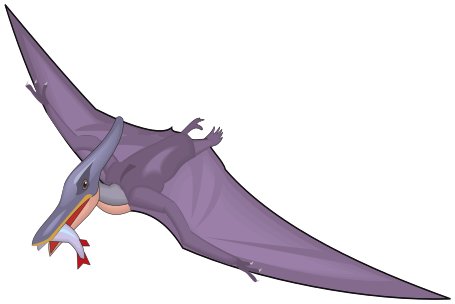
\includegraphics[width=\columnwidth]{Monsters/Animals/Pterosaur}

\subsection{Rat}\index[monsters]{Rat}
\monsterimage{Monsters/Animals/Rat}{\statblock{\textbf{Size:} Small

\textbf{Type:} Animal

\textbf{Habitat:} Any (Common)

\textbf{Wandering Group:} 5d10 (Nil)

\textbf{Lair Group:} 5d10 (L)

\textbf{Move:} 20 ft., 10 ft. (Swim)

\textbf{Armor Class:} 9

\textbf{Hit Dice:} 1 hit point

\textbf{Attacks:} Bite (Special)

\textbf{Special:} Disease

\textbf{Save:} F0

\textbf{Alignment:} None

\textbf{Intelligence:} 2

\textbf{Morale:} 5

\textbf{XP Value:} 2}}

Rats are omnivorous rodents, who are adept at learning and have a very well developed direction sense.

Normally, rats will not attack large creatures unless magically controlled.

In combat, rats should be split into groups of 5-10 individuals. Each group will attack a single target, and can collectively bite for 1d6 damage. If enough rats are killed that a group is no longer viable, those rats will disperse.

\textbf{Disease:} Rat bites have a 1 in 20 chance of transmitting a disease. If this is the case, the victim is affected as if by a Cause Disease spell (complete with saving throw).

\subsection{Rhagodessa, Giant}\index[monsters]{Giant Rhagodessa}
\statblock{\textbf{Size:} Large

\textbf{Type:} Animal

\textbf{Habitat:} Hills, Mountains, Underground, Woods (Rare)

\textbf{Wandering Group:} 1d4 (U)

\textbf{Lair Group:} 1d6 (Nil)

\textbf{Move:} 50 ft.

\textbf{Armor Class:} 5

\textbf{Hit Dice:} 4+2 (20 HP)

\textbf{Attacks:} Leg (Special) \& Bite (2d8)

\textbf{Special:} Leg Grab

\textbf{Save:} F2

\textbf{Alignment:} None

\textbf{Intelligence:} 0

\textbf{Morale:} 9

\textbf{XP Value:} 125}

A giant rhagodessa is an arachnid similar to a spider or scorpion. They are nocturnal hunters, that will attack any prey smaller than themselves.

Rhagodessas do not have stings or create webs, but their front legs end in suckers for holding prey.

\textbf{Leg Grab:} Anyone hit by a rhagodessa's leg will be automatically pulled to their mouth and bitten in the next round.

\subsection{Robber Fly, Giant}\index[monsters]{Giant Robber Fly}
\statblock{\textbf{Size:} Small

\textbf{Type:} Animal

\textbf{Habitat:} Clear, Mountains, Underground, Woods (Rare)

\textbf{Wandering Group:} 1d6 (U)

\textbf{Lair Group:} 2d6 (Nil)

\textbf{Move:} 30 ft., 60 ft. (Fly)

\textbf{Armor Class:} 6

\textbf{Hit Dice:} 2 (9 HP)

\textbf{Attacks:} Bite (1d8)

\textbf{Special:} Immunity to Giant Bee Poison

\textbf{Save:} F1

\textbf{Alignment:} None

\textbf{Intelligence:} 0

\textbf{Morale:} 8

\textbf{XP Value:} 20}

A giant robber fly is an insect with yellow and black stripes. Although it closely resembles a giant bee or wasp, it is not related to those and has no sting.

Giant robber flies mostly prey on giant bees.

When they encounter larger creatures, they will usually hide. If their hiding place is disturbed, they will leap out and attack the intruder, surprising on a 1-4 on 1d6.

\subsection{Roc}\index[monsters]{Roc}
\statblock{\textbf{Size:} Large

\textbf{Type:} Animal

\textbf{Habitat:} Mountains (Rare)

\textbf{Wandering Group:} 0 (Nil)

\textbf{Lair Group:} 1d8 (I)

\textbf{Move:} 20 ft., 160 ft. (Fly)

\textbf{Armor Class:} 2

\textbf{Hit Dice:} 12 (54 HP)

\textbf{Attacks:} 2x Claw (1d8) \& Bite (2d10)

\textbf{Special:} None

\textbf{Save:} F6

\textbf{Alignment:} None

\textbf{Intelligence:} 2

\textbf{Morale:} 9

\textbf{XP Value:} 1,250}

A roc is an eagle-like bird.

Rocs are very territorial, and will chase other large predators out of their areas.

\subsection{Rockroach}\index[monsters]{Rockroach}

\statblock{\textbf{Size:} Small

\textbf{Type:} Monster

\textbf{Habitat:} Underground (Common)

\textbf{Wandering Group:} 1d4 (V)

\textbf{Lair Group:} 1d4 (Nil)

\textbf{Move:} 20 ft.

\textbf{Armor Class:} 2

\textbf{Hit Dice:} 3+1* (15 HP)

\textbf{Attacks:} Bite (1d6)

\textbf{Special:} Paralyzing Gaze

\textbf{Save:} F3

\textbf{Alignment:} None

\textbf{Intelligence:} 2

\textbf{Morale:} 7

\textbf{XP Value:} 75}

Rockroaches are squat creatures with a hard stony carapace like that of a horseshoe crab. When motionless they look exactly like boulders.

Rockroaches are peaceful creatures that prefer to live in natural caverns near water and eat the mosses, fungi and lichens that grow there. If they are disturbed they will lift up their carapace to reveal glowing eyes.

\textbf{Paralyzing Gaze:} Once per round, a rockroach can gaze at a target and cause that target to be paralyzed for 2d4 rounds unless they can make a saving throw vs. paralysis.

If the rockroaches manage to paralyze all opponents, or the opponents retreat, the rockroaches will back off themselves.

However, if the opponents continue to attack, rockroaches will defend themselves by biting and continuing to attempt to paralyze foes. If forced into self defense like this, rockroaches will not simply leave paralyzed opponents to recover, but will kill them.

\subsection{Rust Monster}\index[monsters]{Rust Monster}
\statblock{\textbf{Size:} Medium

\textbf{Type:} Monster

\textbf{Habitat:} Underground (Rare)

\textbf{Wandering Group:} 1d4 (Nil)

\textbf{Lair Group:} 1d4 (Nil)

\textbf{Move:} 40 ft.

\textbf{Armor Class:} 2

\textbf{Hit Dice:} 5* (23 HP)

\textbf{Attacks:} Touch (Special)

\textbf{Special:} Rust

\textbf{Save:} F3

\textbf{Alignment:} None

\textbf{Intelligence:} 2

\textbf{Morale:} 7

\textbf{XP Value:} 300}

A rust monster appears like an armadillo with a long tail and two feathery antennae on its head.

Rust monsters normally eat rusted metal or metal ores. They are particularly attracted to the smell of refined metal, and usually attempt to rust and eat it.

If well treated and regularly fed, rust monsters can be trained to attack only strangers. Such trained rust monsters are sometimes kept by tribes or individuals who fear armed attack by others.

\textbf{Rust:} The antennae of a rust monster will rust any metal they contact. A successful attack on a target with a metal weapon or shield or wearing metal armor means that one of those items has been touched and will immediately crumble to powdered rust. A rust monster will normally try to rust weapons first, to minimize the danger to itself.

If an item is magical, it has a 10\% chance per magical “plus” of resisting the effect.

\subsection{Salamander, Flame}\index[monsters]{Flame Salamander}
\statblock{\textbf{Size:} Large

\textbf{Type:} Dragon

\textbf{Habitat:} Desert, Volcanic, Elemental Plane of Fire (Very Rare)

\textbf{Wandering Group:} 1d4+1 (Nil)

\textbf{Lair Group:} 2d4 (F)

\textbf{Move:} 40 ft.

\textbf{Armor Class:} 2*

\textbf{Hit Dice:} 8* (36 HP)

\textbf{Attacks:} 2x Claw (1d4) \& Bite (1d8)

\textbf{Special:} Aura of Heat, Immunity (Fire, Normal Weapons)

\textbf{Save:} F8

\textbf{Alignment:} None

\textbf{Intelligence:} 1

\textbf{Morale:} 8

\textbf{XP Value:} 1,200}

Fire salamanders are bright red amphibians that radiate great heat.

\textbf{Aura of Heat:} Flame salamanders radiate a great amount of heat, doing 1d8 points of fire damage to all creatures within 20 feet.

\subsection{Salamander, Frost}\index[monsters]{Frost Salamander}
\statblock{\textbf{Size:} Large

\textbf{Type:} Dragon

\textbf{Habitat:} Arctic, Elemental Plane of Air (Very Rare)

\textbf{Wandering Group:} 1d3 (Nil)

\textbf{Lair Group:} 1d3 (E)

\textbf{Move:} 40 ft.

\textbf{Armor Class:} 3*

\textbf{Hit Dice:} 12* (54 HP)

\textbf{Attacks:} 4x Claw (1d4) \& Bite (2d6)

\textbf{Special:} Aura of Cold, Immunity (Cold, Normal Weapons)

\textbf{Save:} F12

\textbf{Alignment:} None

\textbf{Intelligence:} 1

\textbf{Morale:} 9

\textbf{XP Value:} 2,125}

Frost salamanders are six legged amphibians that grow to 20 feet long.

In combat, a frost salamander will rear up onto its back two legs and attack with all four front and middle legs.

\textbf{Aura of Cold:} Frost salamanders radiate an intense cold that does 1d8 damage per round to all within 20 feet.

\subsection{Sasquatch}\index[monsters]{Sasquatch}
\monsterimage[-.5]{Monsters/Yeti}{\statblock{\textbf{Size:} Large

\textbf{Type:} Humanoid

\textbf{Habitat:} Arctic, Mountains, Woods (Rare)

\textbf{Wandering Group:} 0 (Nil)

\textbf{Lair Group:} 1d10 (Nil)

\textbf{Move:} 50 ft.

\textbf{Armor Class:} 6

\textbf{Hit Dice:} 5* (23 HP)

\textbf{Attacks:} 2x Claw (2d4)

\textbf{Special:} Hug, 

Rock Throwing

\textbf{Save:} F5

\textbf{Alignment:} Neutral

\textbf{Intelligence:} 6

\textbf{Morale:} 6

\textbf{XP Value:} 300}}

Sasquatches are powerfully built ape-like humanoids with long fur that changes from brown to white depending on the season.

Sasquatches are not normally aggressive except in self defense, and have been known to rescue lost travelers and guide them to safety.

\textbf{Hug:} When enraged, a sasquatch will attack with its claws, and if both claws hit the same opponent it will hug the opponent for 4d6 damage.

\textbf{Rock Throwing:} Sasquatches can throw rocks (range: 50/75/100) at opponents who are outside melee range. A successful attack inflict 2d8 damage.

\subsubsection{Spellcasting}
Sasquatches can be shamans (to \nth{4} level) or sorcerers (to \nth{2} level).

\subsubsection{As a Class}\index[classes]{Sasquatch}
Sasquatches can be used as a class using the following statistics:

\statblock{\textbf{Ability Requirements:} Strength 10, Constitution 5

\textbf{Prime Requisite:} Strength, Dexterity, Intelligence, or Wisdom

\textbf{Ability Modifiers:} Strength +2, Intelligence -1

\textbf{Weapons:} Any

\textbf{Armor:} Any

\textbf{Natural AC:} 8

\textbf{Special Abilities:} Hug, Rock Throwing

\textbf{Magic Item Use:} Fighter}

\begin {table}[H]
  \caption{Sasquatch Progression}
  \begin{tabularx}{\columnwidth}{>{\bfseries}YYY}
  \thead{Level} & \thead{Experience} & \thead{Hit Dice}\\
	-3 & -6,000 & 2d8\\
	-2 & -4,000 & 3d8\\
	-1 & -2,000 & 4d8\\
	0 & 0 & 5d8\\
	1 & 6,000 & 6d8\\
	2 & 12,000 & 7d8\\
	3 & 24,000 & 8d8\\
	4 & 48,000 & 9d8\\
	5 & 96,000 & 10d8\\
	6 & 192,000 & 11d8\\
	7 & 384,000 & 12d8\\
	8 & 768,000 & 13d8\\
	9+ & +300,000 & +2 HP
  \end {tabularx}
\end {table}

\subsection{Scorpion, Giant}\index[monsters]{Giant Scorpion}
\statblock{\textbf{Size:} Medium

\textbf{Type:} Animal

\textbf{Habitat:} Desert, Underground (Rare)

\textbf{Wandering Group:} 1d6 (V)

\textbf{Lair Group:} 1d6 (Nil)

\textbf{Move:} 50 ft.

\textbf{Armor Class:} 2

\textbf{Hit Dice:} 4* (18 HP)

\textbf{Attacks:} 2x Claw (1d10) \& Sting (1d4)

\textbf{Special:} Poison

\textbf{Save:} F2

\textbf{Alignment:} None

\textbf{Intelligence:} 0

\textbf{Morale:} 11

\textbf{XP Value:} 125}

Giant scorpions are aggressive hunters. They hunt by grasping creatures in its claws and stinging them. If either claw attack hits an opponent, the giant scorpion gets a +2 bonus to hit that same opponent with its stinger.

\textbf{Poison:} Anyone stung by a giant scorpion must make a saving throw vs. poison or die.

\subsection{Scorpionfolk}\index[monsters]{Scorpionfolk}
\statblock{\textbf{Size:} Large

\textbf{Type:} Monster

\textbf{Habitat:} Desert, Mountains, Underground (Rare)

\textbf{Wandering Group:} 1d8 (V)

\textbf{Lair Group:} 2d10 (J, K,Mx2)

\textbf{Move:} 80 ft.

\textbf{Armor Class:} 1

\textbf{Hit Dice:} 8*** (36 HP)

\textbf{Attacks:} Weapon (By weapon) \& Sting (1d10)

\textbf{Special:} Poison

\textbf{Save:} F8

\textbf{Alignment:} Chaotic

\textbf{Intelligence:} 8

\textbf{Morale:} 10

\textbf{XP Value:} 2,300}

Scorpionfolk are xenophobic and isolationist humanoids. They are similar to centaurs, having a human body with arms and head coming forth from the body of a giant scorpion.

\textbf{Poison:} Anyone stung by a scorpionfolk must make a saving throw vs. poison or die. Even if the saving throw is made, any creature not immune to paralysis or poison will still be paralyzed for 1d8-1 rounds.

\subsubsection{Spellcasting}
Scorpionfolk can be shamans (to \nth{13} level) or sorcerers (to \nth{8} level).

\subsubsection{As a Class}\index[classes]{Scorpionfolk}
Scorpionfolk can be used as a class using the following statistics:

\textbf{Cleric Abilities:} At \nth{8} level and higher, scorpionfolk can use all \iref[class:Cleric]{Cleric} abilities as a \iref[class:Cleric]{Cleric} of 7 levels lower.

\textbf{Landlubber:} The anatomy of a scorpionfolk makes it impossible for them to swim. Although, with their additional legs they are able to move 3/4 their normal speed on the ground beneath the water.

\statblock{\textbf{Ability Requirements:} Strength 13

\textbf{Prime Requisite:} Strength

\textbf{Ability Modifiers:} None

\textbf{Weapons:} Any

\textbf{Armor:} Any (2/3 the AC due to not being able to wear the bottom half)

\textbf{Natural AC:} 4

\textbf{Special Abilities:} Cleric Spells, Landlubber, Poison, Turn Undead

\textbf{Magic Item Use:} Fighter}

\begin {table}[H]
  \caption{Scorpionfolk Progression}
  \begin{tabularx}{\columnwidth}{>{\bfseries}YYY}
  \thead{Level} & \thead{Experience} & \thead{Hit Dice}\\
	-7 & -156,000 & 1d8\\
	-6 & -83,200 & 2d8\\
	-5 & -41,600 & 3d8\\
	-4 & -20,800 & 4d8\\
	-3 & -10,400 & 5d8\\
	-2 & -5,200 & 6d8\\
	-1 & -2,600 & 7d8\\
	0 & 0 & 8d8\\
	1 & 2,600 & 9d8\\
	2 & 5,200 & 10d8\\
	3 & 10,400 & 11d8\\
	4 & 20,800 & 12d8\\
	5 & 41,600 & 13d8\\
	6 & 83,200 & 14d8\\
	7 & 156,000 & 15d8\\
	8 & 312,000 & 16d6\\
	9 & 468,000 & 17d6\\
	10+ & +200,000 & +2 HP
  \end {tabularx}
\end {table}

\subsection{Shadow}\index[monsters]{Shadow}
\statblock{\textbf{Size:} Medium

\textbf{Type:} Monster

\textbf{Habitat:} Underground, Woods (Rare)

\textbf{Wandering Group:} 1d8 (Nil)

\textbf{Lair Group:} 1d12 (F)

\textbf{Move:} 30 ft.

\textbf{Armor Class:} 7

\textbf{Hit Dice:} 2+2* (11 HP)

\textbf{Attacks:} Touch (1d4)

\textbf{Special:} Blend, Drain Strength

\textbf{Save:} F2

\textbf{Alignment:} Chaotic

\textbf{Intelligence:} 4

\textbf{Morale:} 12

\textbf{XP Value:} 35}

Shadows are dark and incorporeal barely sapient creatures that lurk in corners and cellars. They look very much like a real shadow.

Despite their appearance, shadows are not undead and cannot be turned.

\textbf{Blend:} Shadows are difficult to see and can surprise opponents on a roll of 1-5 on 1d6.

\textbf{Drain Strength:} Anyone touched by a shadow loses 1 point of \iref[sec:Strength]{Strength}. This weakness lasts for an hour. If an opponent is drained to zero \iref[sec:Strength]{Strength}, they immediately become a shadow themselves.

\subsection{Shark, Bull}\index[monsters]{Bull Shark}
\statblock{\textbf{Size:} Medium

\textbf{Type:} Animal

\textbf{Habitat:} Ocean (Common)

\textbf{Wandering Group:} 0 (Nil)

\textbf{Lair Group:} 3d6 (Nil)

\textbf{Move:} 60 ft.

\textbf{Armor Class:} 4

\textbf{Hit Dice:} 2* (9 HP)

\textbf{Attacks:} Bite (2d4)

\textbf{Special:} Charge

\textbf{Save:} F1

\textbf{Alignment:} None

\textbf{Intelligence:} 2

\textbf{Morale:} 7

\textbf{XP Value:} 25}

Bull sharks are brown sharks.

\textbf{Charge:} Bull sharks can make a Charge attack, which does no damage but forces their opponent to make a saving throw vs. paralysis or be \iref[sec:Stunned]{Stunned} for three rounds.

\subsection{Shark, Great White}\index[monsters]{Great White Shark}
\statblock{\textbf{Size:} Large

\textbf{Type:} Animal

\textbf{Habitat:} Ocean (Rare)

\textbf{Wandering Group:} 0 (Nil)

\textbf{Lair Group:} 1d4 (Nil)

\textbf{Move:} 60 ft.

\textbf{Armor Class:} 4

\textbf{Hit Dice:} 8 (36 HP)

\textbf{Attacks:} Bite (2d10)

\textbf{Special:} None

\textbf{Save:} F4

\textbf{Alignment:} None

\textbf{Intelligence:} 2

\textbf{Morale:} 7

\textbf{XP Value:} 650}

Great white sharks are among the biggest of sharks, reaching 30’ long.

They are sometimes known to attack small boats.

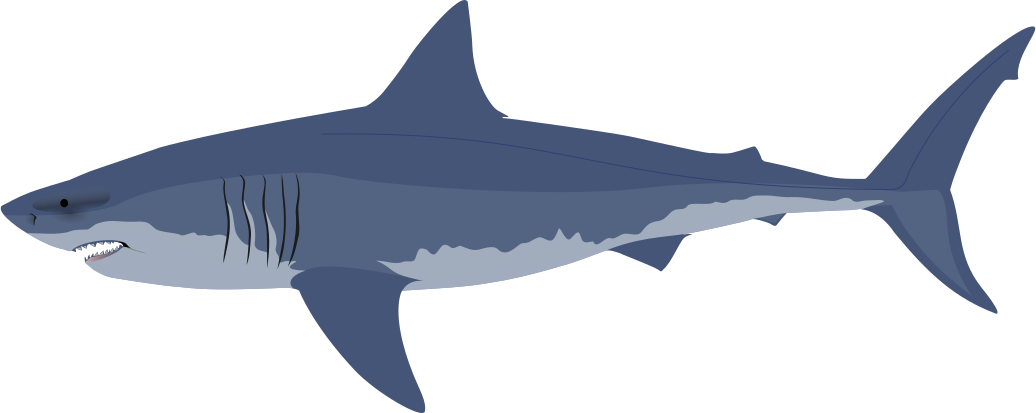
\includegraphics[width=\columnwidth]{Monsters/Animals/Shark, Great White}

\subsection{Shark, Mako}\index[monsters]{Mako Shark}
\statblock{\textbf{Size:} Large

\textbf{Type:} Animal

\textbf{Habitat:} Ocean (Common)

\textbf{Wandering Group:} 0 (Nil)

\textbf{Lair Group:} 2d6 (Nil)

\textbf{Move:} 60 ft.

\textbf{Armor Class:} 4

\textbf{Hit Dice:} 4 (18 HP)

\textbf{Attacks:} Bite (2d6)

\textbf{Special:} None

\textbf{Save:} F2

\textbf{Alignment:} None

\textbf{Intelligence:} 2

\textbf{Morale:} 7

\textbf{XP Value:} 75}

Mako sharks are notoriously unpredictable, attacking or changing opponents without apparent reason.

\subsection{Shrew, Giant}\index[monsters]{Giant Shrew}
\statblock{\textbf{Size:} Small

\textbf{Type:} Animal

\textbf{Habitat:} Clear, Underground, Woods (Rare)

\textbf{Wandering Group:} 1d4 (Nil)

\textbf{Lair Group:} 1d8 (Nil)

\textbf{Move:} 60 ft., 5 ft (Burrow), 5 ft. (Jump)

\textbf{Armor Class:} 4

\textbf{Hit Dice:} 1* (5 HP)

\textbf{Attacks:} 2x Bite (1d6)

\textbf{Special:} Despair

\textbf{Save:} F1

\textbf{Alignment:} None

\textbf{Intelligence:} 2

\textbf{Morale:} 10

\textbf{XP Value:} 13}

Giant shrews are rat-like brown-furred animals with long snouts. Their diet consists of insects and vegetable matter.

Giant shrews have weak vision, forcing them to rely on their hearing for movement. They squeak and listen for echoes which allows them to sense any creature within a 60 ft. radius. This can only be used in enclosed areas. If a giant shrew is in an open area they will have trouble getting around. If the surrounding area is affected by a Silence 15-foot radius spell, the giant shrew will become confused and suffers a +4 to their AC and a -4 to their attack rolls.

Giant shrews are very quick which allows them to attack first on the first round of combat. They gain a +1 initiative on all remaining rounds of combat.

Giant shrews are so nervous and aggressive that they will attack anything that comes within 20 ft. of them. They attack by ferociously biting a victims face, head, and shoulders.

\textbf{Despair:} Any victim of 3 HD or less that suffers the ferocious attack of a giant shrew must make a saving throw vs. death ray or run in fear.

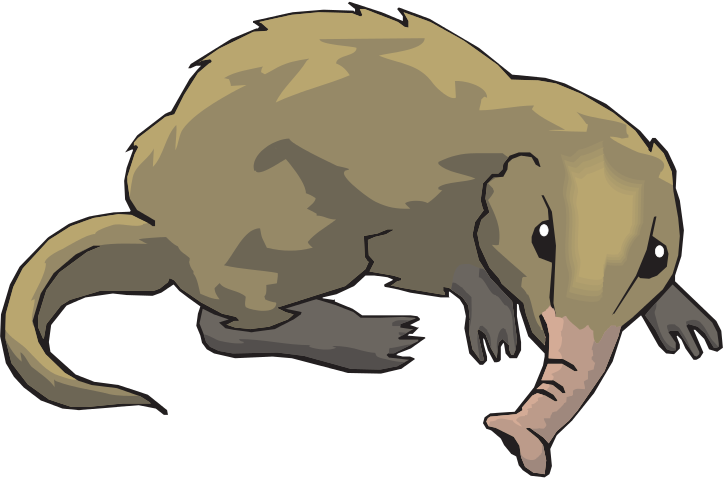
\includegraphics[width=\columnwidth]{Monsters/Animals/Shrew, Giant}

\subsection{Shrieker}\index[monsters]{Shrieker}
\statblock{\textbf{Size:} Medium

\textbf{Type:} Plant

\textbf{Habitat:} Underground (Common)

\textbf{Wandering Group:} 0 (Nil)

\textbf{Lair Group:} 1d8 (Nil)

\textbf{Move:} 3 ft.

\textbf{Armor Class:} 7

\textbf{Hit Dice:} 3 (14 HP)

\textbf{Attacks:} Special

\textbf{Special:} Shriek

\textbf{Save:} F2

\textbf{Alignment:} None

\textbf{Intelligence:} 0

\textbf{Morale:} 12

\textbf{XP Value:} 35}

Shriekers are large toadstool-like fungi that live underground and slowly move around looking for detritus to eat.

Because their shrieking unwittingly makes them into very effective guards, shriekers are often deliberately cultivated by underground races.

\textbf{Shriek:} When disturbed by light within 60 feet or movement within 30 feet, shriekers emit a piercing scream which lasts for 1d3 rounds.

The scream of a shrieker will stun animals of rat-size or smaller, which the shrieker will then engulf and eat.

\subsection{Sidhe}\index[monsters]{Sidhe}
\statblock{\textbf{Size:} Medium

\textbf{Type:} Fey

\textbf{Habitat:} Any (Rare)

\textbf{Wandering Group:} 1d4 (Nil)

\textbf{Lair Group:} 1d100 (A)

\textbf{Move:} 40 ft.

\textbf{Armor Class:} By Armor

\textbf{Hit Dice:} 1/2 (2 HP)

\textbf{Attacks:} Weapon (By weapon)

\textbf{Special:} Susceptibility to Iron, Water Breathing

\textbf{Save:} F0

\textbf{Alignment:} Any

\textbf{Intelligence:} 10

\textbf{Morale:} 7

\textbf{XP Value:} 7}

Sidhe appear almost human-like, with only their slightly elven features making them distinguishable.

Like humans, sidhe are adaptable making them natural leaders.

\textbf{Susceptibility to Iron:} Sidhe are allergic to iron. When handling iron for an extended period of time, it begins to make them sick. For every hour a sidhe handles iron, they suffer 1 hit point of damage.

\textbf{Water Breathing:} Sidhe can breathe underwater.

\subsubsection{As a Class}\index[classes]{Sidhe}
Sidhe can be used as a class using the following statistics:

\textbf{Fey Spells:} Sidhe can cast fey spells. See \fullref{sec:Spell Descriptions} for detailed descriptions of these spells.

\textbf{Fighter/Rogue Abilities:} During character creation, sidhe must choose to have all the abilities of a fighter or a rogue. This choice effects the sidhe's hit dice, prime requisite, and weapons and armor use.

\statblock{\textbf{Ability Requirements:} Strength 8, Intelligence 8

\textbf{Prime Requisite:} Strength or Dexterity (Str for Fighter abilities, Dex for Rogue abilities), Intelligence

\textbf{Ability Modifiers:} None

\textbf{Weapons:} Any non-iron (Fighter Abilities), Any non-iron one-handed and any non-iron missile (Rogue Abilities)

\textbf{Armor:} Any non-iron (Fighter Abilities), Leather armor (Rogue Abilities)

\textbf{Special Abilities:} Fey Spells, Fighter/Rogue Abilities

\textbf{Magic Item Use:} Fighter or Rogue (Depending on Abilities)}

\begin {table}[H]
  \caption{Sidhe Progression}
  \begin{tabularx}{\columnwidth}{>{\bfseries}YYY}
  \thead{Level} & \thead{Experience} & \thead{Hit Dice}\\
	0 & 0 & 1d4\\
	1 & 2,500 & 1d4+1d4\\
	2 & 5,000 & 2d4\\
	3 & 10,000 & 3d4\\
	4 & 20,000 & 4d4\\
	5 & 40,000 & 5d4\\
	6 & 80,000 & 6d4\\
	7 & 160,000 & 7d4\\
	8 & 320,000 & 8d4\\
	9 & 620,000 & 9d4\\
	10+ & +300,000 & +1 HP
  \end {tabularx}
\end {table}

\begin {table}[H]
  \caption{Sidhe Spells per Day by Spell Level}
  \begin{tabularx}{\columnwidth}{>{\bfseries}YYYYYYYY}
	\thead{} & \multicolumn{7}{c}{\thead{Spell Level}}\\
	\thead{Level} & \thead{1} & \thead{2} & \thead{3} & \thead{4} & \thead{5} & \thead{6} & \thead{7}\\
	1 & 1 & - & - & - & - & - & -\\
	2 & 2 & - & - & - & - & - & -\\
	3 & 2 & 1 & - & - & - & - & -\\
	4 & 2 & 2 & - & - & - & - & -\\
	5 & 3 & 2 & - & - & - & - & -\\
	6 & 3 & 2 & 1 & - & - & - & -\\
	7 & 3 & 2 & 2 & - & - & - & -\\
	8 & 3 & 3 & 2 & - & - & - & -\\
	9 & 3 & 3 & 2 & 1 & - & - & -\\
	10 & 3 & 3 & 2 & 2 & - & - & -\\
	11 & 3 & 3 & 3 & 2 & - & - & -\\
	12 & 3 & 3 & 3 & 2 & 1 & - & -\\
	13 & 3 & 3 & 3 & 2 & 2 & - & -\\
	14 & 3 & 3 & 3 & 3 & 2 & - & -\\
	15 & 3 & 3 & 3 & 3 & 2 & 1 & -\\
	16 & 3 & 3 & 3 & 3 & 2 & 2 & -\\
	17 & 3 & 3 & 3 & 3 & 3 & 2 & -\\
	18 & 3 & 3 & 3 & 3 & 3 & 2 & 1\\
	19 & 3 & 3 & 3 & 3 & 3 & 2 & 2\\
	20 & 3 & 3 & 3 & 3 & 3 & 3 & 3\\
	21 & 4 & 4 & 3 & 3 & 3 & 3 & 3\\
	22 & 4 & 4 & 4 & 4 & 3 & 3 & 3\\
	23 & 4 & 4 & 4 & 4 & 4 & 4 & 3\\
	24 & 4 & 4 & 4 & 4 & 4 & 4 & 4\\
	25 & 5 & 5 & 4 & 4 & 4 & 4 & 4\\
	26 & 5 & 5 & 5 & 5 & 4 & 4 & 4\\
	27 & 5 & 5 & 5 & 5 & 5 & 5 & 4\\
	28 & 5 & 5 & 5 & 5 & 5 & 5 & 5\\
	29 & 6 & 6 & 5 & 5 & 5 & 5 & 5\\
	30 & 6 & 6 & 6 & 6 & 5 & 5 & 5\\
	31 & 6 & 6 & 6 & 6 & 6 & 6 & 5\\
	32 & 6 & 6 & 6 & 6 & 6 & 6 & 6\\
	33 & 7 & 7 & 6 & 6 & 6 & 6 & 6\\
	34 & 7 & 7 & 7 & 7 & 6 & 6 & 6\\
	35 & 7 & 7 & 7 & 7 & 7 & 7 & 6\\
	36 & 7 & 7 & 7 & 7 & 7 & 7 & 7
  \end {tabularx}
\end {table}

\subsection{Skeleton}\index[monsters]{Skeleton}
\statblock{\textbf{Size:} Medium

\textbf{Type:} Undead

\textbf{Habitat:} Underground (Common)

\textbf{Wandering Group:} 3d4 (Nil)

\textbf{Lair Group:} 3d10 (Nil)

\textbf{Move:} 20 ft.

\textbf{Armor Class:} 7

\textbf{Hit Dice:} 1 (5 HP)

\textbf{Attacks:} Weapon (By weapon)

\textbf{Special:} Immunity (Mind Effects, Poison)

\textbf{Save:} F1

\textbf{Alignment:} None

\textbf{Intelligence:} 1

\textbf{Morale:} 12

\textbf{XP Value:} 10}

Animated skeletons are the weakest and most basic of undead creatures, and often work as servants and minions to more powerful undead or spellcasters.

Although unintelligent, skeletons do have basic instincts, and can react to novel situations.

\subsection{Slime, Fire}\index[monsters]{Fire Slime}
\statblock{\textbf{Size:} Large

\textbf{Type:} Ooze

\textbf{Habitat:} Underground (Very Rare)

\textbf{Wandering Group:} 1d3 (Nil)

\textbf{Lair Group:} 2d4 (Nil)

\textbf{Move:} 30 ft.

\textbf{Armor Class:} 5

\textbf{Hit Dice:} 9 (41 HP)

\textbf{Attacks:} 3x Bash (4d6)

\textbf{Special:} Amorphous, Immunity (Fire, Mental Attacks), 

Residue, Sense Movement

\textbf{Save:} F9

\textbf{Alignment:} None

\textbf{Intelligence:} 0

\textbf{Morale:} 12

\textbf{XP Value:} 900}

Fire slime is a bright red/orange glowing gelatinous ooze that is incredibly hot.

Fire slime will mindlessly attack any creatures it detects.

Fire slime take double damage from all cold-based attacks.

\textbf{Amorphous:} As it is semi-liquid, fire slime are able to pass through small cracks and fissures.

\textbf{Residue:} When a fire slime hits an opponent, it leaves a layer of hot slime on them. This layer of slime does 3d6 fire damage per round for a further 1d4 rounds.

If the fire slime hits a target again before the previous slime has burnt out then the fire damage does not stack but the duration before it burns out does.

\textbf{Sense Movement:} Fire slime can sense movement within 60 feet.

\subsection{Slime, Green}\index[monsters]{Green Slime}
\statblock{\textbf{Size:} Medium

\textbf{Type:} Ooze

\textbf{Habitat:} Underground (Common)

\textbf{Wandering Group:} 1 (P+S)

\textbf{Lair Group:} 1 (B)

\textbf{Move:} 1 ft.

\textbf{Armor Class:} Special*

\textbf{Hit Dice:} 2** (9 HP)

\textbf{Attacks:} Special

\textbf{Special:} Engulf

\textbf{Save:} F1

\textbf{Alignment:} None

\textbf{Intelligence:} 0

\textbf{Morale:} 7

\textbf{XP Value:} 30}

A green slime is an ooze of a virulent green color. It can crawl up walls and along ceilings, and will often drop from ceilings in a surprise attack.

Green slime can be automatically hit by any attack, although it can only be harmed by fire and cold attacks. A Cure Disease spell will kill a green slime with no saving throw.

\textbf{Engulf:} If a green slime hits an opponent, it starts to dissolve their clothing and armor. Leather or cloth can be dissolved in a single round, wood or metal in six rounds. Once a green slime has dissolved its victims armor or clothing, it will dissolve the victim in 1d4 rounds turning it into more green slime.

While a green slime is engulfing a victim, any fire or cold attack done to it will do half damage to the slime and half damage to the victim. Attacks with an area of effect (for example Fireball spells) will do full damage to both slime and victim.

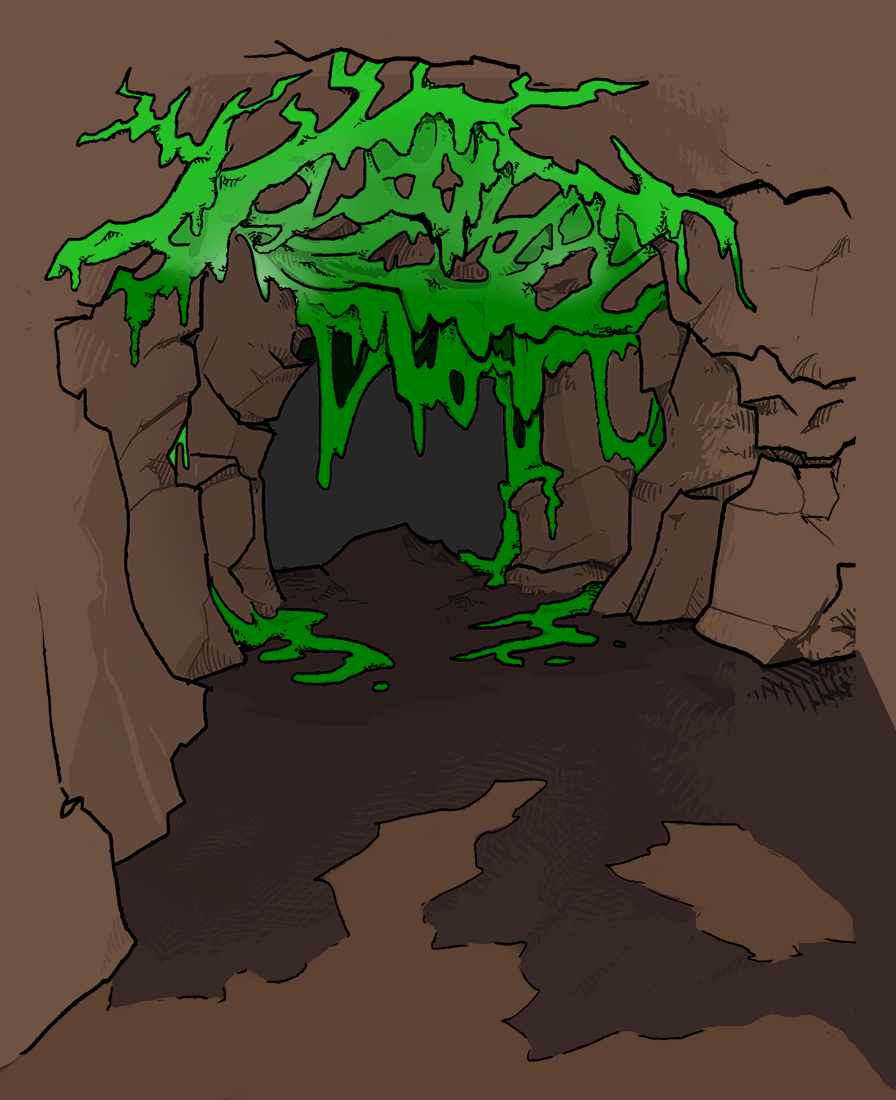
\includegraphics[width=\columnwidth]{Monsters/Green Slime}

\subsection{Snake, Constrictor}\index[monsters]{Constrictor Snake}
\statblock{\textbf{Size:} Large

\textbf{Type:} Animal

\textbf{Habitat:} Jungle, Swamp (Common)

\textbf{Wandering Group:} 1d3 (Nil)

\textbf{Lair Group:} 1d3 (Nil)

\textbf{Move:} 30 ft.

\textbf{Armor Class:} 6

\textbf{Hit Dice:} 5* (22 HP)

\textbf{Attacks:} Bite (1d4)

\textbf{Special:} Squeeze

\textbf{Save:} F3

\textbf{Alignment:} None

\textbf{Intelligence:} 2

\textbf{Morale:} 7

\textbf{XP Value:} 300}

Constrictor snakes are non-poisonous snakes that squeeze their prey to death.

\textbf{Squeeze:} With a successful bite, a rock python will coil around the victim and squeeze for 2d4 points of damage.

The snake will then cease biting, and automatically squeeze for 2d4 damage per round until slain.

\subsection{Snake, Sea}\index[monsters]{Sea Snake}
\statblock{\textbf{Size:} Medium

\textbf{Type:} Animal

\textbf{Habitat:} Ocean (Common)

\textbf{Wandering Group:} 0 (Nil)

\textbf{Lair Group:} 1d8 (Nil)

\textbf{Move:} 30 ft.

\textbf{Armor Class:} 6

\textbf{Hit Dice:} 3* (14 HP)

\textbf{Attacks:} Bite (1)

\textbf{Special:} Poison

\textbf{Save:} F2

\textbf{Alignment:} None

\textbf{Intelligence:} 2

\textbf{Morale:} 7

\textbf{XP Value:} 50}

Sea snakes live in the sea and rarely if ever venture onto land.

\textbf{Poison:} When a sea snake bites an opponent, the opponent must make a saving throw vs. poison or will die in 1d4+2x10 minutes. There is a 50\% chance that the poisoned bite may not be noticed by the opponent, as the sea snake's bite feels like a pin prick.

\subsection{Snake, Poisonous}\index[monsters]{Poisonous Snake}
\monsterimage{Monsters/Animals/Snake, Poisonous}{\statblock{\textbf{Size:} Small

\textbf{Type:} Animal

\textbf{Habitat:} Any except Arctic (Common)

\textbf{Wandering Group:} 1d6 (Nil)

\textbf{Lair Group:} 1d6 (Nil)

\textbf{Move:} 30 ft.

\textbf{Armor Class:} 7

\textbf{Hit Dice:} 1* (5 HP)

\textbf{Attacks:} Bite (1d3)

\textbf{Special:} Poison, Spit

\textbf{Save:} F1

\textbf{Alignment:} None

\textbf{Intelligence:} 2

\textbf{Morale:} 7

\textbf{XP Value:} 13}}

Poisonous snakes are snakes that have poison glands and fangs.

\textbf{Poison:} When a poisonous snake bites an opponent, the opponent must make a saving throw vs. poison or will die in 1d10x10 minutes.

\subsubsection{Spitting Cobra}\index[monsters]{Spitting Cobra}
Spitting cobras are brownish poisonous snakes that can spit their venom.

\textbf{Spit:} Spitting cobras can spit a stream of venom up to 10 feet into a target’s eyes. The target must make a saving throw vs. poison or be \iref[sec:Blinded]{Blinded} until cured.

\subsection{Snake, Racer}\index[monsters]{Racer Snake}
\statblock{\textbf{Size:} Medium

\textbf{Type:} Animal

\textbf{Habitat:} Any (Common)

\textbf{Wandering Group:} 1d6 (Nil)

\textbf{Lair Group:} 1d8 (Nil)

\textbf{Move:} 40 ft.

\textbf{Armor Class:} 5

\textbf{Hit Dice:} 2 (9 HP)

\textbf{Attacks:} Bite (1d6)

\textbf{Special:} None

\textbf{Save:} F1

\textbf{Alignment:} None

\textbf{Intelligence:} 2

\textbf{Morale:} 7

\textbf{XP Value:} 20}

Racer snakes are not poisonous, relying on their fast speed to catch small prey.

A racer will bite larger opponents in self defense, but is not normally aggressive.

\subsection{Spectral Hound}\index[monsters]{Spectral Hound}
\statblock{\textbf{Size:} Medium

\textbf{Type:} Extraplanar

\textbf{Habitat:} Any (Very Rare)

\textbf{Wandering Group:} 1d6 (Nil)

\textbf{Lair Group:} 1d6 (Nil)

\textbf{Move:} 50 ft.

\textbf{Armor Class:} -2

\textbf{Hit Dice:} 5** (23 HP)

\textbf{Attacks:} Bite (2d6)

\textbf{Special:} Fade, Immunity (Cold, Fire, Normal Weapons)

\textbf{Save:} F5

\textbf{Alignment:} None

\textbf{Intelligence:} 3

\textbf{Morale:} 12

\textbf{XP Value:} 425}

Spectral hounds are ghostly dogs with dark eyes. Although they may appear similar to undead, they are from a far away plane.

\textbf{Fade:} Any creature bitten by a spectral hound must make a saving throw vs. spells or begin to fade away. This process takes 24 hours, by which point the victim is completely faded and incorporeal (treat as if having drunk a Potion of Gaseous Form).

This fading is permanent, although a faded character is likely to starve to death—being unable to eat solid food—in only a few days.

The only way to counteract the fading once it has started is with a Dimension Door spell. The faded victim can walk through the door into the real world again.

\subsection{Spectre}\index[monsters]{Spectre}
\statblock{\textbf{Size:} Medium

\textbf{Type:} Undead

\textbf{Habitat:} Underground (Rare)

\textbf{Wandering Group:} 1d4 (Nil)

\textbf{Lair Group:} 1d8 (E)

\textbf{Move:} 50 ft., 100 ft. (Fly)

\textbf{Armor Class:} 2*

\textbf{Hit Dice:} 6** (27 HP)

\textbf{Attacks:} Touch (1d8)

\textbf{Special:} Create Spawn, Energy Drain, 

Immunity (Mind Effects, Normal Weapons, Poison)

\textbf{Save:} F6

\textbf{Alignment:} Chaotic

\textbf{Intelligence:} 8

\textbf{Morale:} 11

\textbf{XP Value:} 725}

Spectres are incorporeal undead creatures, that appear as translucent humanoid figures with glowing eyes.

\textbf{Create Spawn:} Anyone slain by a spectre will rise the following night as another spectre unless raised.

\textbf{Energy Drain:} Anyone touched by a spectre is subject to a double strength \iref[sec:Energy Drain]{Energy Drain} that drains them of two levels (no saving throw).

\subsection{Sphinx}\index[monsters]{Sphinx}
\statblock{\textbf{Size:} Large

\textbf{Type:} Monster

\textbf{Habitat:} Desert (Rare)

\textbf{Wandering Group:} 1d2 (Nil)

\textbf{Lair Group:} 1d4 (E)

\textbf{Move:} 60 ft., 120 ft. (Fly)

\textbf{Armor Class:} 0*

\textbf{Hit Dice:} 12***** (54 HP)

\textbf{Attacks:} 2x Claw (3d6) \& Bite (2d8)

\textbf{Special:} Cleric/Wizard Spells, Immunity 

(Normal Weapons, Spells < \nth{4} level), Roar

\textbf{Save:} F24

\textbf{Alignment:} Any

\textbf{Intelligence:} 13

\textbf{Morale:} 10

\textbf{XP Value:} 5,625}

Sphinxes are winged lions with human faces.

Sphinxes love riddles, puzzles and trivia; and can often be dissuaded from attacking by trading them new bits and pieces that they have not heard before.

\textbf{Cleric/Wizard Spells:} All sphinxes are powerful spellcasters: female sphinxes can cast spells as a \nth{12} level cleric, and males as a \nth{12} level wizard. All saving throws made against spells cast by sphinxes have a -4 penalty.

\textbf{Roar:} Twice per day, a sphinx can roar instead of attacking. All within 120 feet must save vs. spells with a -4 penalty of flee in terror for 1d6x10 minutes. All within 60 feet must additionally save vs. paralysis or be \iref[sec:Stunned]{Stunned}  for 1d6 rounds. All within 10 feet must make both saving throws and also take 6d6 damage and are deafened for 1d10x10 minutes (no save).

\subsubsection{As a Class}\index[classes]{Sphinx}
Sphinxes can be used as a class using the following statistics:

\statblock{\textbf{Ability Requirements:} Strength 6, Intelligence 6, Wisdom 8

\textbf{Prime Requisite:} Constitution and Wisdom

\textbf{Ability Modifiers:} None

\textbf{Weapons:} None

\textbf{Armor:} None

\textbf{Natural AC:} 2

\textbf{Special Abilities:} Cleric/Wizard Spells, Roar

\textbf{Magic Item Use:} Male: Wizard (Non-Weapon), Female: Cleric (Non-Weapon)}

\begin {table}[H]
  \caption{Sphinx Progression}
  \begin{tabularx}{\columnwidth}{>{\bfseries}YYY}
  \thead{Level} & \thead{Experience} & \thead{Hit Dice}\\
	-10 & -3,000,000 & 2d8\\
	-9 & -2,700,000 & 3d8\\
	-8 & -2,400,000 & 4d8\\
	-7 & -2,100,000 & 5d8\\
	-6 & -1,800,000 & 6d8\\
	-5 & -1,500,000 & 7d8\\
	-4 & -1,200,000 & 8d8\\
	-3 & -900,000 & 9d8\\
	-2 & -600,000 & 10d8\\
	-1 & -300,000 & 11d8\\
	0 & 0 & 12d8\\
	1 & 300,000 & 13d8\\
	2 & 600,000 & 14d8\\
	3 & +300,000 & +2 HP
  \end {tabularx}
\end {table}

\subsection{Spider, Giant Black Widow}\index[monsters]{Giant Black Widow}
\monsterimage{Monsters/Animals/Spider, Giant Black Widow}{\statblock{\textbf{Size:} Medium

\textbf{Type:} Animal

\textbf{Habitat:} Underground, Woods (Rare)

\textbf{Wandering Group:} 1d3 (U)

\textbf{Lair Group:} 1d3 (Nil)

\textbf{Move:} 20 ft., 40 ft. (In Web)

\textbf{Armor Class:} 6

\textbf{Hit Dice:} 3* (14 HP)

\textbf{Attacks:} Bite (2d6)

\textbf{Special:} Poison

\textbf{Save:} F2

\textbf{Alignment:} None

\textbf{Intelligence:} 0

\textbf{Morale:} 8

\textbf{XP Value:} 50}}

Giant black widow are black with a distinctive red hour-glass shaped marking.

The web of a giant black widow spider should be treated as if a Web spell.

\textbf{Poison:} Anyone bitten by a black widow spider must make a saving throw vs. poison or die in 10 minutes.

\subsection{Spider, Giant Crab}\index[monsters]{Giant Crab Spider}
\statblock{\textbf{Size:} Medium

\textbf{Type:} Animal

\textbf{Habitat:} Underground (Rare)

\textbf{Wandering Group:} 1d4 (U)

\textbf{Lair Group:} 1d4 (U)

\textbf{Move:} 40 ft.

\textbf{Armor Class:} 7

\textbf{Hit Dice:} 2* (9 HP)

\textbf{Attacks:} Bite (1d8)

\textbf{Special:} Blend, Poison

\textbf{Save:} F1

\textbf{Alignment:} None

\textbf{Intelligence:} 0

\textbf{Morale:} 7

\textbf{XP Value:} 25}

Giant crab spiders are spiders with a gray color.

Giant crab spiders don’t build webs, but hide in corners and drop or leap out in ambush of prey, surprising on a 1-4 on 1d6.

\textbf{Blend:} The giant crab spider's gray color makes them extremely difficult to spot on stone surfaces, allowing them to surprise opponents on a 1-4.

\textbf{Poison:} Anyone bitten by a giant crab spider must make a saving throw vs. poison with a +2 bonus or die in 1d4x10 minutes.

\subsection{Spider, Giant Tarantella}\index[monsters]{Giant Tarantella}
\monsterimage{Monsters/Animals/Spider, Giant Tarantula}{\statblock{\textbf{Size:} Medium

\textbf{Type:} Animal

\textbf{Habitat:} Underground, Woods (Rare)

\textbf{Wandering Group:} 1d3 (U)

\textbf{Lair Group:} 1d3 (Nil)

\textbf{Move:} 40 ft.

\textbf{Armor Class:} 5

\textbf{Hit Dice:} 4* (18 HP)

\textbf{Attacks:} Bite (1d8)

\textbf{Special:} Poison

\textbf{Save:} F2

\textbf{Alignment:} None

\textbf{Intelligence:} 0

\textbf{Morale:} 8

\textbf{XP Value:} 125}}

Giant tarantellas are hairy spiders.

They do not use webs, but are mobile and aggressively hunt.

\textbf{Poison:} Anyone bitten by a giant tarantella must make a saving throw vs. poison or start to have painful spasms which resemble dancing.

Anyone seeing this dance must make a saving throw vs. spells or join in, dancing in the same manner.

Dancing characters have a -4 on attack rolls and give their opponents +4 on their attack rolls.

The dance can be stopped with a Dispel Magic spell, or it will wear off in 2d6x10 minutes. However, dancers will drop from exhaustion after 50 minutes of dancing.

\subsection{Spider, Huge Wood}\index[monsters]{Huge Wood Spider}\label{Huge Wood Spider}
\statblock{\textbf{Size:} Medium

\textbf{Type:} Animal

\textbf{Habitat:} Woods (Common) 

\textbf{Wandering Group:} 1d4 (Nil)

\textbf{Lair Group:} 4d4 (U)

\textbf{Move:} 40 ft.

\textbf{Armor Class:} 6

\textbf{Hit Dice:} 1+3* (7 HP)

\textbf{Attacks:} Bite (1d6)

\textbf{Special:} Camouflage, Poison

\textbf{Save:} F1

\textbf{Alignment:} Neutral

\textbf{Intelligence:} 2

\textbf{Morale:} 8

\textbf{XP Value:} 19}

Huge wood spiders are 3 foot long spiders that are green with jagged brown stripes.

\textbf{Camouflage:} The huge wood spider's markings provide remarkably effective camouflage in wooded surroundings, causing the huge wood spider to surprise their opponents on a 1-4 on 1d6.

\textbf{Poison:} Anyone bitten by a huge wood spider must make a saving throw vs. poison with a +2 bonus or suffer 1d8 points of damage and become \iref[sec:Sluggish]{Sluggish} for 2d4+2 rounds.

\subsection{Spider, Ice}\index[monsters]{Ice Spider}
\statblock{\textbf{Size:} Medium

\textbf{Type:} Monster

\textbf{Habitat:} Elemental Plane of Water (Very Rare)

\textbf{Wandering Group:} 1 (Nil)

\textbf{Lair Group:} 1 (F)

\textbf{Move:} 20 ft., 60 ft. (Swim)

\textbf{Armor Class:} 2*

\textbf{Hit Dice:} 7**

\textbf{Attacks:} 2x Claw (1d10) or Special

\textbf{Special:} Immunity (Fire, Normal Weapons, 

Spells < \nth{3} level), Spell-like Abilities

\textbf{Save:} F14

\textbf{Alignment:} Lawful

\textbf{Intelligence:} 9

\textbf{Morale:} 9

\textbf{XP Value:} 1,250}

Ice spiders are large intelligent spiders that are entirely made of ice. Ice spiders are coldly logical creatures that show no compassion or mercy to others who get in their way, and seem to have no imagination.

\textbf{Spell-like Abilities:} An ice spider can cast the following spells as if a \nth{9} level caster: \iref[spell:Detect Invisible]{Detect Invisible} (at will), \iref[spell:Detect Magic]{Detect Magic} (at will), \iref[spell:Web]{Web} (at will), \iref[spell:Dispel Magic]{Dispel Magic} (at will), \iref[spell:Ice Storm/Wall of Ice]{Ice Storm/Wall of Ice} (at will), \ilink{spell:Water to Ice}{Water to Ice} (3/day), and \iref[spell:Ice to Water]{Ice to Water} (3/day).

\subsection{Spider, Phase}\index[monsters]{Phase Spider}
\statblock{\textbf{Size:} Medium

\textbf{Type:} Extraplanar

\textbf{Habitat:} Any (Very Rare)

\textbf{Wandering Group:} 2d6 (Nil)

\textbf{Lair Group:} 3d6 (Nil)

\textbf{Move:} 60 ft.

\textbf{Armor Class:} 6

\textbf{Hit Dice:} 5** (23 HP)

\textbf{Attacks:} Bite (2d6)

\textbf{Special:} Poison

\textbf{Save:} F5

\textbf{Alignment:} Any

\textbf{Intelligence:} 12

\textbf{Morale:} 9

\textbf{XP Value:} 425}

Phase spiders are intelligent and magical spiders. They can shift between the \ilink{sec:Prime Plane}{Prime Plane} and the \iref[sec:Ethereal Plane]{Ethereal Plane} at will.

In combat, a phase spider will appear in the \ilink{sec:Prime Plane}{Prime Plane} immediately after the Statement of Intent phase, and then disappear back to the \iref[sec:Ethereal Plane]{Ethereal Plane} once it has made its attack on its initiative. It is therefore only vulnerable to attacks from people who both beat its initiative and were able to correctly predict where it would appear (possibly by delaying their statement of intent until after the spider’s statement of intent).

\textbf{Poison:} Anyone bitten by a phase spider must save vs. poison or die, although the spider can withhold its venom if it chooses.

\subsubsection{Spellcasting}
Phase spiders are as varied in personality as humans. They can become shamans (to \nth{9} level) or sorcerers (to \nth{9} level).

\subsection{Spirit}
\textbf{Aura of Spoilage:} The chilling aura around a spirit is enough to spoil consumable items within 30 feet, including food potions and even holy water. Spoiled goods are no longer edible but are not poisonous. Plants and insects in the area are paralyzed (and therefore cannot be magically controlled) and will die if in the aura for more than an hour.

\textbf{Immunity to Spells < \nth{4} level:} Spirits are immune to all magic spells of less than \nth{4} level.

\textbf{Immunity to Weapons < +2:} Spirits are only hurt by +2 or better weapons.

\textbf{Poison:} Anyone touched by a spirit must make a saving throw vs. poison or die.

\textbf{Spell-like Abilities:} Spirits can use the following spells as if a \nth{16} level caster: \iref[spell:Detect Invisible]{Detect Invisible} (constant), \ilink{spell:Darkness}{Darkness} (at will), \iref[spell:Silence 15-foot radius]{Silence 15-foot radius} (at will), \ilink{spell:Cause Disease}{Cause Disease} (at will), \iref[spell:Animate Dead]{Animate Dead} (at will), and \ilink{spell:Finger of Death}{Finger of Death} (at will).

\subsubsection{Druj}\index[monsters]{Druj}
\statblock{\textbf{Size:} Medium

\textbf{Type:} Undead

\textbf{Habitat:} Any (Very Rare)

\textbf{Wandering Group:} 1 (I, O, V)

\textbf{Lair Group:} 0 (Nil)

\textbf{Move:} 30 ft.

\textbf{Armor Class:} -4*

\textbf{Hit Dice:} 14**** (63 HP)

\textbf{Attacks:} Eye: Special; Hand: Claw (1d4); Skull: Bite (2d4) 

\textbf{Special:} Aura of Spoilage, Clone Self, 

Immunity (Mind Effects, Poison, Spells < \nth{4} level, Weapons < +2), 

Paralyzing Gaze (Eye), Paralyzing Presence (Skull), 

Poison, Spell-like Abilities, Squeeze (Hand)

\textbf{Save:} F14

\textbf{Alignment:} Chaotic

\textbf{Intelligence:} 14

\textbf{Morale:} 11

\textbf{XP Value:} 5,500}

A druj spirit takes the form of an animated body part; either a skeletal hand, an eye or a skull.

A druj travels from place to place by night, as it is powerless during the day.

\textbf{Clone Self:} Once per night, a druj can split itself into four identical copies. Each of these has the physical capabilities of the druj, but only one has the spellcasting capabilities.

If the spellcasting copy of the druj is slain, one of the other copies becomes the new “master” copy and gains the ability to cast spells.

If a druj is turned by a cleric while split, the pieces must immediately rejoin and can not split again until the following night.

\textbf{Paralyzing Gaze:} An eye druj may gaze at one opponent per round within 30 feet, who must make a saving throw vs. paralysis or be paralyzed for 1d4x10 minutes.

\textbf{Paralyzing Presence:} When opponents first encounter a skull druj, they must make a saving throw vs. spells or be paralyzed with fear for 2d6 rounds.

\textbf{Squeeze:} If a hand druj claws a target, it holds on to its victim automatically doing damage equal to the armor class of the victim (ignoring \iref[sec:Dexterity]{Dexterity} bonus) + 1d4 damage. If the adjusted armor class bonus is negative, the druj still does 1d4 damage per round.

\subsubsection{Odic}\index[monsters]{Odic}
\statblock{\textbf{Size:} As Plant

\textbf{Type:} Undead

\textbf{Habitat:} Any (Very Rare)

\textbf{Wandering Group:} 1 (I, O, V)

\textbf{Lair Group:} 0 (Nil)

\textbf{Move:} Special

\textbf{Armor Class:} -4*

\textbf{Hit Dice:} 16**** (72 HP)

\textbf{Attacks:} Branch (1d12)

\textbf{Special:} Aura of Draining, Aura of Spoilage, 

Immunity (Mind Effects, Poison, Spells < \nth{4} level, 

Weapons < +2), Poison, Reach, Spell-like Abilities

\textbf{Save:} F16

\textbf{Alignment:} Chaotic

\textbf{Intelligence:} 12

\textbf{Morale:} 12

\textbf{XP Value:} 6,250}

An odic spirit travels incorporeally each day, settling into a plant (preferably a tree) at night.

Once an odic has chosen its plant, it can no longer move until morning; when it will leave in incorporeal form to find another plant.

\textbf{Aura of Draining:} When an odic possesses a plant, the plant immediately dies, and radiates a purplish glow in a 20-foot radius. Anyone entering this glow must make a saving throw vs. spells or be affected by an \iref[sec:Energy Drain]{Energy Drain}.

\textbf{Reach:} The odic can make up to 6 leaves, needles, flowers, or other plant parts fly at 30 feet per round for up to 1 mile from the plant in search of victims. Each of these can touch (attack bonus +4) a creature causing it to make a saving throw vs. spells or be entranced and attempt to reach the odic’s plant host; suffering a -4 on the saving throw against the plant’s level draining aura. Because of the seemingly innocuous nature of the plant parts, they surprise victims on a 1-5 on 1d6.

\subsubsection{Revenant}\index[monsters]{Revenant}
\statblock{\textbf{Size:} As Plant

\textbf{Type:} Undead

\textbf{Habitat:} Any (Very Rare)

\textbf{Wandering Group:} 1 (I, O, V)

\textbf{Lair Group:} 0 (Nil)

\textbf{Move:} 40 ft.

\textbf{Armor Class:} -3*

\textbf{Hit Dice:} 18**** (81 HP)

\textbf{Attacks:} 2x Claw (2d4) \& Bite (1d4+2)

\textbf{Special:} Aura of Spoilage, Immunity (Mind Effects, 

Poison, Spells < \nth{4} level, Weapons < +2), Leap Attack, Poison, 

Resistance to Turning, Spell-like Abilities, Summon Spectres

\textbf{Save:} F18

\textbf{Alignment:} Chaotic

\textbf{Intelligence:} 13

\textbf{Morale:} 10

\textbf{XP Value:} 7,525}

A revenant appears much like a zombie, although it moves much more quickly and may leap up to 60 feet once per 10 minutes.

\textbf{Leap Attack:} When first encountered, a revenant will pretend to be a zombie, and then suddenly make a surprise leap attack. This attack will surprise its opponents on a 1-3 on 1d6, and if the target of the leap is surprised then all three attacks automatically hit.

\textbf{Resistance to Turning:} Revenants are particularly resistant to being turned. If a cleric gets a ‘D’ result when turning a revenant, the revenant may make a saving throw vs. spells to avoid the effect. If a cleric gets a normal turning result, the turn effect only lasts for 1d4 rounds before the revenant recovers.

\textbf{Summon Spectres:} Once per night, a revenant can summon 1d4 spectres to its aid. They arrive within 1d6+2 rounds of being summoned.

\subsection{Sprite}\index[monsters]{Sprite}
\statblock{\textbf{Size:} Small

\textbf{Type:} Fey

\textbf{Habitat:} Woods (Common)

\textbf{Wandering Group:} 3d6 (S)

\textbf{Lair Group:} 5d8 (Nil)

\textbf{Move:} 20 ft., 60 ft. (Fly)

\textbf{Armor Class:} 5

\textbf{Hit Dice:} 1/2 (3 HP)

\textbf{Attacks:} Special

\textbf{Special:} Curse

\textbf{Save:} E1

\textbf{Alignment:} Neutral

\textbf{Intelligence:} 14

\textbf{Morale:} 7

\textbf{XP Value:} 6}

Sprites are winged fey, related to pixies.

Sprites are rather shy, but are very curious and have a keen sense of humor and enjoy playing practical jokes.

Sprites never fight. If threatened, they will flee.

Sprites can be very kind and helpful when not being silly, and will often look after children who get lost in woods and protect them from danger.

\textbf{Curse:} Five sprites working together can cast a Curse spell, although the effects will always be funny rather than dangerous. The spell can be removed as normal by a Remove Curse, or the sprites can remove it at will.

\subsubsection{Spellcasting}
Sprites can be shamans (to \nth{6} level) or sorcerers (to \nth{4} level).

\subsubsection{As a Class}\index[classes]{Sprite}
Sprites can be used as a class using the following statistics:

\textbf{Fey Spells:} Sprites can cast fey spells. See \fullref{sec:Spell Descriptions} for detailed descriptions of these spells.

\statblock{\textbf{Ability Requirements:} Dexterity 13, Intelligence 9

\textbf{Prime Requisite:} Dexterity and Intelligence

\textbf{Ability Modifiers:} None

\textbf{Weapons:} Daggers, small trident

\textbf{Armor:} None

\textbf{Natural AC:} 8

\textbf{Special Abilities:} Curse, Fey Spells

\textbf{Magic Item Use:} Fighter}

\begin {table}[H]
  \caption{Sprite Progression}
  \begin{tabularx}{\columnwidth}{>{\bfseries}YYY}
  \thead{Level} & \thead{Experience} & \thead{Hit Dice}\\
	0 & 0 & 1d4\\
	1 & 2,000 & 2d4\\
	2 & 4,000 & 3d4\\
	3 & 8,000 & 4d4\\
	4 & 16,000 & 5d4\\
	5 & 32,000 & 6d4\\
	6 & 64,000 & 7d4\\
	7 & 128,000 & 8d4\\
	8 & 250,000 & 9d4\\
	9 & 500,000 & 10d4\\
	10+ & +300,000 & +1 HP
  \end {tabularx}
\end {table}


\begin {table}[H]
  \caption{Sprite Spells per Day by Spell Level}
  \begin{tabularx}{\columnwidth}{>{\bfseries}YYYYYYYY}
	\thead{} & \multicolumn{7}{c}{\thead{Spell Level}}\\
	\thead{Level} & \thead{1} & \thead{2} & \thead{3} & \thead{4} & \thead{5} & \thead{6} & \thead{7}\\
	1 & 1 & - & - & - & - & - & -\\
	2 & 2 & - & - & - & - & - & -\\
	3 & 2 & 1 & - & - & - & - & -\\
	4 & 2 & 2 & - & - & - & - & -\\
	5 & 2 & 2 & 1 & - & - & - & -\\
	6 & 2 & 2 & 2 & - & - & - & -\\
	7 & 2 & 2 & 2 & 1 & - & - & -\\
	8 & 3 & 2 & 2 & 2 & - & - & -\\
	9 & 3 & 2 & 2 & 2 & 1 & - & -\\
	10 & 3 & 3 & 2 & 2 & 2 & - & -\\
	11 & 3 & 3 & 3 & 2 & 2 & 1 & -\\
	12 & 4 & 3 & 3 & 2 & 2 & 2 & -\\
	13 & 4 & 4 & 3 & 2 & 2 & 2 & 1\\
	14 & 4 & 4 & 3 & 3 & 3 & 2 & 1\\
	15 & 4 & 4 & 4 & 3 & 3 & 2 & 2\\
	16 & 4 & 4 & 4 & 4 & 4 & 3 & 2\\
	17 & 4 & 4 & 4 & 4 & 4 & 3 & 3\\
	18 & 4 & 4 & 4 & 4 & 4 & 4 & 4\\
	19 & 5 & 5 & 5 & 4 & 4 & 4 & 4\\
	20 & 5 & 5 & 5 & 5 & 5 & 4 & 4\\
	21 & 5 & 5 & 5 & 5 & 5 & 5 & 5\\
	22 & 6 & 6 & 5 & 5 & 5 & 5 & 5\\
	23 & 6 & 6 & 6 & 6 & 5 & 5 & 5\\
	24 & 6 & 6 & 6 & 6 & 6 & 6 & 5\\
	25 & 6 & 6 & 6 & 6 & 6 & 6 & 6\\
	26 & 7 & 7 & 7 & 6 & 6 & 6 & 6\\
	27 & 7 & 7 & 7 & 7 & 7 & 6 & 6\\
	28 & 7 & 7 & 7 & 7 & 7 & 7 & 7\\
	29 & 8 & 8 & 7 & 7 & 7 & 7 & 7\\
	30 & 8 & 8 & 8 & 8 & 7 & 7 & 7\\
	31 & 8 & 8 & 8 & 8 & 8 & 8 & 7\\
	32 & 8 & 8 & 8 & 8 & 8 & 8 & 8\\
	33 & 9 & 9 & 8 & 8 & 8 & 8 & 8\\
	34 & 9 & 9 & 9 & 9 & 8 & 8 & 8\\
	35 & 9 & 9 & 9 & 9 & 9 & 9 & 8\\
	36 & 9 & 9 & 9 & 9 & 9 & 9 & 9
  \end {tabularx}
\end {table}

\subsection{Stirge}\index[monsters]{Stirge}
\statblock{\textbf{Size:} Small

\textbf{Type:} Monster

\textbf{Habitat:} Underground, Woods (Common)

\textbf{Wandering Group:} 1d10 (Nil)

\textbf{Lair Group:} 3d12 (L)

\textbf{Move:} 10 ft., 60 ft. (Fly)

\textbf{Armor Class:} 7

\textbf{Hit Dice:} 1* (5 HP)

\textbf{Attacks:} Bite (1d3)

\textbf{Special:} Blood Drain

\textbf{Save:} F2

\textbf{Alignment:} None

\textbf{Intelligence:} 1

\textbf{Morale:} 9

\textbf{XP Value:} 13}

Stirges are flying creatures that look like a cross between a giant mosquito and a crow.

Stirges get +2 to hit on their initial attack, because of their quick diving flight.

\textbf{Blood Drain:} If a stirge’s bite succeeds, it will attach themselves to the victim and begin to drain their blood out through their long pointed beak. The victim suffers 1d3 points of damage for every round their blood is being drained. The stirge will continue to drain the victim's blood until either the stirge or the victim is dies.

\subsection{Termite, Giant Water}\index[monsters]{Giant Water Termite}
\begin {table}[H]
	\normalsize
	\begin{tabularx}{\columnwidth}{@{}>{\bfseries}XXXX@{}}
	\hiderowcolors
	& \textbf{Freshwater} & \textbf{Saltwater} & \textbf{Swamp}\\
	Size: & Small & Medium & Small\\
	Type: & Animal & Animal & Animal\\
	Habitat: & River & Ocean & Swamp\\
	& (Common) & (Common) & (Common)\\
	Wandering Group: & 0 (Nil) & 0 (Nil) & 0 (Nil)\\
	Lair Group: & 1d3 (Nil) & 1d6+1 (Nil) & 1d4 (Nil)\\
	Move: & 40 ft. & 60 ft. & 30 ft.\\
	Armor Class: & 6 & 5 & 4\\
	Hit Dice: & 2+1 (11 HP) & 4 (18 HP) & 1+1 (6 HP)\\
	Attacks: & Bite (1d3) & Bite (1d6) & Bite (1d4)\\
	Special: & None & None & None\\
	Save: & F2 & F3 & F1\\
	Alignment: & None & None & None\\
	Intelligence: & 9 & 0 & 9\\
	Morale: & 8 & 11 & 10\\
	XP Value: & 25 & 75 & 15\\
	\showrowcolors
  \end {tabularx}
\end {table}

Giant water termites appear like normal termites except for an elastic abdomen that fills up with water and then propels them forward by squeezing a jet out.

Giant water termites are not normally aggressive towards swimmers, but they will attack ships or rafts made of wood.

The bite of a giant water termite does full damage to ships, piers, and other wooden structures.

\subsection{Toad, Giant}\index[monsters]{Giant Toad}
\statblock{\textbf{Size:} Small

\textbf{Type:} Animal

\textbf{Habitat:} River, Underground (Common)

\textbf{Wandering Group:} 1d4 (Nil)

\textbf{Lair Group:} 1d6 (Nil)

\textbf{Move:} 30 ft.

\textbf{Armor Class:} 7

\textbf{Hit Dice:} 2+2 (11 HP)

\textbf{Attacks:} Bite (1d4+1)

\textbf{Special:} Blend, Tongue Grab

\textbf{Save:} F1

\textbf{Alignment:} None

\textbf{Intelligence:} 2

\textbf{Morale:} 6

\textbf{XP Value:} 25}

\textbf{Blend:} The giant toad's mottled skin makes them hard to see in poorly lit situations. In such areas, they surprise opponents on a roll of 1-3 on 1d6.

\textbf{Tongue Grab:} Giant toads can shoot their tongues 15 feet and anything dwarf sized or smaller hit by the tongue will be dragged into the toads mouth and automatically bitten.

\subsection{Treant}\index[monsters]{Treant}
\monsterimage{Monsters/Treant}{
\statblock{\textbf{Size:} Large

\textbf{Type:} Plant

\textbf{Habitat:} Woods (Rare)

\textbf{Wandering Group:} 0 (Nil)

\textbf{Lair Group:} 1d8 (C)

\textbf{Move:} 20 ft.

\textbf{Armor Class:} 2

\textbf{Hit Dice:} 8* (36 HP)

\textbf{Attacks:} 2x Branch (2d6)

\textbf{Special:} Animate Trees, 

Treeshape

\textbf{Save:} F8

\textbf{Alignment:} Lawful

\textbf{Intelligence:} 11

\textbf{Morale:} 9

\textbf{XP Value:} 1,200}}

A treant is an intelligent and mobile tree. Its trunk is split into two legs with rooty feet.

Treants care for the trees and animals of their forest, and are allies to most forest creatures.

\textbf{Animate Trees:} A treant can animate two normal trees within 60 feet to move and fight as treants. The treant may choose to change which trees it is animating each round.

\textbf{Treeshape:} Treants can only be distinguished from normal trees from distances of less than 90 feet, and even then the treant can surprise opponents on a 1-3 on 1d6.

\subsubsection{Spellcasting}
Treants can be shamans (to \nth{12} level).

\subsubsection{As a Class}\index[classes]{Treant}
Treants can be used as a class using the following statistics:

\textbf{Create Potion:} At \nth{10} level, treants are able to create potions as a wizard. They tend to create common potions, such as a Potion of Healing from components gathered from the forest.

\textbf{Ability Requirements:} Strength 10, Constitution 8, Wisdom 6

\statblock{\textbf{Prime Requisite:} Constitution

\textbf{Ability Modifiers:} None

\textbf{Weapons:} Any

\textbf{Natural Attacks:} 2x Branch (1d6 [Immature -3], 1d8 [Immature -2], 1d10 [Immature -1], 1d12 [Mature])

\textbf{Armor:} None

\textbf{Natural AC:} 8 (Immature -3), 6 (Immature -2), 4 (Immature -1), 2 (Mature)

\textbf{Special Abilities:} Animate Trees, Treeshape, Create Potion

\textbf{Magic Item Use:} Fighter}

\begin {table}[H]
  \caption{Treant Progression}
  \begin{tabularx}{\columnwidth}{>{\bfseries}YYY}
  \thead{Level} & \thead{Experience} & \thead{Hit Dice}\\
	-3 & -48,000 & 2d8\\
	-2 & -36,500 & 4d8\\
	-1 & -24,000 & 6d8\\
	0 & 0 & 8d8\\
	1 & 48,000 & -\\
	2 & 145,000 & 9d8\\
	3 & 340,000 & -\\
	4 & 640,000 & 10d8\\
	5 & 940,000 & -\\
	6 & 1,240,000 & 11d8\\
	7 & 1,540,000 & -\\
	8 & 1,840,000 & 12d8\\
	9+ & +300,000 & +3 HP
  \end {tabularx}
\end {table}

\subsection{Triton}\index[monsters]{Triton}
\statblock{\textbf{Size:} Medium

\textbf{Type:} Humanoid

\textbf{Habitat:} Ocean (Rare)

\textbf{Wandering Group:} 10d6 (Nil)

\textbf{Lair Group:} 0 (F [5 HD], G [6 HD], or H [7 HD])

\textbf{Move:} 50 ft. (Swim)

\textbf{Armor Class:} 6 (5 HD), 5 (6 HD), 4 (7 HD)

\textbf{Hit Dice:} 5***, 6***, or 7****

\textbf{Attacks:} Weapon (By weapon)

\textbf{Special:} Cleric/Wizard Spells

\textbf{Save:} D11

\textbf{Alignment:} Neutral

\textbf{Intelligence:} 11

\textbf{Morale:} 9

\textbf{XP Value:} 550 (5 HD), 950 (6 HD), 2,050 (7 HD)}

Tritons have human torsos and fish-like tails. Their skin is silver-blue and their hair is deep blue or blue-green. Tritons braid their hair and decorate their bodies with shells.

Tritons live in large coral cities on the ocean floor. These cities are arranged beautifully as if a work of art. Tritons use giant sea horses as transportation.

\textbf{Cleric/Wizard Spells:} There is a 50\% chance that a triton can cast spells as either a \iref[class:Cleric]{Cleric} or \iref[class:Wizard]{Wizard} of level equivalent to the triton's hit dice.

\subsubsection{As a Class}\index[classes]{Triton}
Tritons can be used as a class using the following statistics:

\textbf{Cleric/Wizard Spells:} During character creation, tritons must choose to have the ability to cast spells as a \iref[class:Cleric]{Cleric}, a \iref[class:Wizard]{Wizard}, or both. This choice effects the triton's ability requirements, prime requisite, ability modifiers and the number of experience points required to reach each level.

\statblock{\textbf{Ability Requirements:} None; Intelligence 15, Wisdom 15 (Cleric and Wizard Spells)

\textbf{Prime Requisite:} Intelligence or Wisdom (Int for Wizard spells, Wis for Cleric spells, Both for Cleric and Wizard spells)

\textbf{Ability Modifiers:} Strength -1, Intelligence or Wisdom (Int for Wizard spells, Wis for Cleric spells, Player's Choice for both)

\textbf{Weapons:} Any

\textbf{Armor:} None

\textbf{Natural AC:} 7

\textbf{Special Abilities:} Cleric/Wizard Spells

\textbf{Magic Item Use:} Cleric, Wizard, or Both (Depending on Spells)}

\begin {table}[H]
  \caption{Triton Progression}
  \begin{tabularx}{\columnwidth}{>{\bfseries}cccYc}
	\thead{} & \multicolumn{3}{c}{\thead{Experience}} & \thead{}\\
	\thead{Level} & \thead{Cleric Spells} & \thead{Wizard Spells} & \thead{Cleric \& Wizard Spells} & \thead{Hit Dice}\\
	-3 & -24,000 & -30,000 & -36,000 & 2d8\\
	-2 & -18,000 & -24,000 & -30,000 & 3d8\\
	-1 & -12,000 & -16,000 & -18,000 & 4d8\\
	0 & 0 & 0 & 0 & 5d8\\
	1 & 24,000 & 30,000 & 36,000 & 6d8\\
	2 & 72,000 & 90,000 & 108,000 & 7d8\\
	3 & 168,000 & 210,000 & 252,000 & -\\
	4 & 360,000 & 450,000 & 540,000 & 8d8\\
	5 & 660,000 & 750,000 & 840,000 & -\\
	6 & 960,000 & 1,050,000 & 1,140,000 & 9d8\\
	7 & 1,260,000 & 1,350,000 & 1,440,000 & -\\
	8 & 1,560,000 & 1,650,000 & 1,740,000 & 10d8\\
	9+ & +300,000 & +300,000 & +300,000 & +2 HP
  \end {tabularx}
\end {table}

\subsection{Troglodyte}\index[monsters]{Troglodyte}
\statblock{\textbf{Size:} Medium

\textbf{Type:} Humanoid

\textbf{Habitat:} Underground (Rare)

\textbf{Wandering Group:} 1d8 (Nil)

\textbf{Lair Group:} 5d8 (A)

\textbf{Move:} 40 ft.

\textbf{Armor Class:} 5

\textbf{Hit Dice:} 2* (9 HP)

\textbf{Attacks:} 2x Claw (1d4) \& Bite (1d4)

\textbf{Special:} Blend, Stench

\textbf{Save:} F2

\textbf{Alignment:} Chaotic

\textbf{Intelligence:} 10

\textbf{Morale:} 9

\textbf{XP Value:} 25}

Troglodytes are intelligent humanoid amphibians with short tails and crests on their heads and arms. They tend to live underground near lakes and rivers.

Troglodytes dislike all other races, and will try to drive out all intruders from their territory; using diplomacy, then stench, then violence, depending on how persistent the intruders are.

\textbf{Blend:} Troglodytes have the ability to change the color of their skin to blend into backgrounds, and can surprise opponents on 1-4 on 1d6.

\textbf{Stench:} Troglodytes can also produce a nauseating stench that affects those within melee range of them. Any creature in melee range must make a saving throw vs. poison or take a -2 penalty to to-hit rolls until they are no longer near a troglodyte.

\subsubsection{Spellcasting}
Troglodytes can be shamans (to \nth{4} level) or sorcerers (to \nth{2} level).

\subsubsection{As a Class}\index[classes]{Troglodyte}
Troglodytes can be used as a class using the following statistics:

\statblock{\textbf{Ability Requirements:} None

\textbf{Prime Requisite:} Strength, Dexterity, Intelligence, or Wisdom

\textbf{Ability Modifiers:} Intelligence -1

\textbf{Weapons:} Any

\textbf{Armor:} Any

\textbf{Natural AC:} 7

\textbf{Special Abilities:} Blend, Stench

\textbf{Magic Item Use:} Fighter}

\begin {table}[H]
  \caption{Troglodyte Progression}
  \begin{tabularx}{\columnwidth}{>{\bfseries}YYY}
  \thead{Level} & \thead{Experience} & \thead{Hit Dice}\\
	-1 & -4,000 & 1d8\\
	0 & 0 & 2d8\\
	1 & 4,000 & 3d8\\
	2 & 8,000 & 4d8\\
	3 & 16,000 & -\\
	4 & 32,000 & 5d8\\
	5 & 64,000 & 6d8\\
	6 & 130,000 & 7d8\\
	7 & 260,000 & -\\
	8 & 520,000 & 8d8\\
	9 & +300,000 & +2 HP
  \end {tabularx}
\end {table}

\subsection{Troll}\index[monsters]{Troll}
\statblock{\textbf{Size:} Large

\textbf{Type:} Humanoid

\textbf{Habitat:} Any (Rare)

\textbf{Wandering Group:} 1d8 (Nil)

\textbf{Lair Group:} 1d8 (D)

\textbf{Move:} 40 ft.

\textbf{Armor Class:} 4

\textbf{Hit Dice:} 6+3* (30 HP)

\textbf{Attacks:} 2x Claw (1d6) \& Bite (1d10)

\textbf{Special:} Regeneration (3)

\textbf{Save:} F6

\textbf{Alignment:} Chaotic

\textbf{Intelligence:} 6

\textbf{Morale:} 10

\textbf{XP Value:} 650}

Trolls are ferociously featured humanoids with sharp teeth and mottled rubber-like skin. They are carnivorous, and love to eat other intelligent races.

\textbf{Regeneration:} Trolls regenerate 3 hit points per round until slain. Damage from fire or acid cannot be regenerated.

\subsubsection{As a Class}\index[classes]{Troll}
Trolls can be used as a class using the following statistics:

\statblock{\textbf{Ability Requirements:} Strength 16

\textbf{Prime Requisite:} Strength, Dexterity, Intelligence, or Wisdom

\textbf{Ability Modifiers:} Strength +2, Dexterity -2, Intelligence -2, Wisdom -2, Charisma -2

\textbf{Weapons:} Any

\textbf{Armor:} Any

\textbf{Natural AC:} 9

\textbf{Special Abilities:} Regeneration

\textbf{Magic Item Use:} Fighter}

\begin {table}[H]
  \caption{Troll Progression}
  \begin{tabularx}{\columnwidth}{>{\bfseries}YYY}
  \thead{Level} & \thead{Experience} & \thead{Hit Dice}\\
	-3 & -35,200 & 3d8+2\\
	-2 & -26,400 & 4d8+2\\
	-1 & -17,600 & 5d8+3\\
	0 & 0 & 6d8+3\\
	1 & 35,200 & 7d8+4\\
	2 & 105,600 & 8d8+4\\
	3 & 246,400 & -\\
	4 & 528,000 & 9d8+5\\
	5 & 828,000 & 10d8+5\\
	6 & 1,128,000 & 11d8+5\\
	7 & 1,428,000 & -\\
	8 & 1,728,000 & 12d8+5\\
	9+ & +300,000 & +2 HP
  \end {tabularx}
\end {table}

\subsection{Undine}\index[monsters]{Undine}
\statblock{\textbf{Size:} Large

\textbf{Type:} Monster

\textbf{Habitat:} Elemental Plane of Water (Very Rare)

\textbf{Wandering Group:} 1 (Nil)

\textbf{Lair Group:} 1 (Nil)

\textbf{Move:} 30 ft., 80 ft. (Swim)

\textbf{Armor Class:} 4*

\textbf{Hit Dice:} 8*** (36 HP)

\textbf{Attacks:} Bash (2d8)

\textbf{Special:} Immunity (Fire, Normal Weapons, Poison, 

Spell < \nth{4} level), Spell-like Abilities, Squeeze

\textbf{Save:} F16

\textbf{Alignment:} Chaotic

\textbf{Intelligence:} 10

\textbf{Morale:} 9

\textbf{XP Value:} 2,300}

An undine is an amorphous creature made of water. It normally takes the form of a snake (on land) or an eel (in the water), but can form tentacles, hands, and other features as it wishes.

Undines are playful and compassionate creatures, who are easily upset by seeing other mistreated.

\textbf{Spell-like Abilities:} Undines can use the following spells as if a \nth{9} level caster: \iref[spell:Detect Invisible]{Detect Invisible} (at will), \iref[spell:Detect Magic]{Detect Magic} (at will), \iref[spell:Web]{Web} (as the normal spell, but made of ice and therefore melts rather than burning, at will), \iref[spell:Dispel Magic]{Dispel Magic} (at will), and \iref[spell:Ice Storm/Wall of Ice]{Ice Storm/Wall of Ice} (3/day).

\textbf{Squeeze:} With a tentacle attack, an undine will wrap the tentacle around the victim and squeeze for 1d10 points of damage.

\subsection{Unicorn}\index[monsters]{Unicorn}
\statblock{\textbf{Size:} Large

\textbf{Type:} Monster

\textbf{Habitat:} Woods (Rare)

\textbf{Wandering Group:} 1d2 (Nil)

\textbf{Lair Group:} 1d8 (Nil)

\textbf{Move:} 80 ft.

\textbf{Armor Class:} 2

\textbf{Hit Dice:} 4* (18 HP)

\textbf{Attacks:} 2x Kick (1d8) \& 

Horn (1d8)

\textbf{Special:} Teleport

\textbf{Save:} F8

\textbf{Alignment:} None

\textbf{Intelligence:} 4

\textbf{Morale:} 7

\textbf{XP Value:} 125}

Unicorns appear to be slender horses with a single horn on their forehead. They are always beautiful and graceful.

Unicorns are shy creatures, and only the gentlest and most patient of people can win their trust. If a unicorn does come to trust a person and let them ride it, at the first sign of cruelty or aggression from its companion (to any creature not just the unicorn itself), the unicorn will leave and never return.

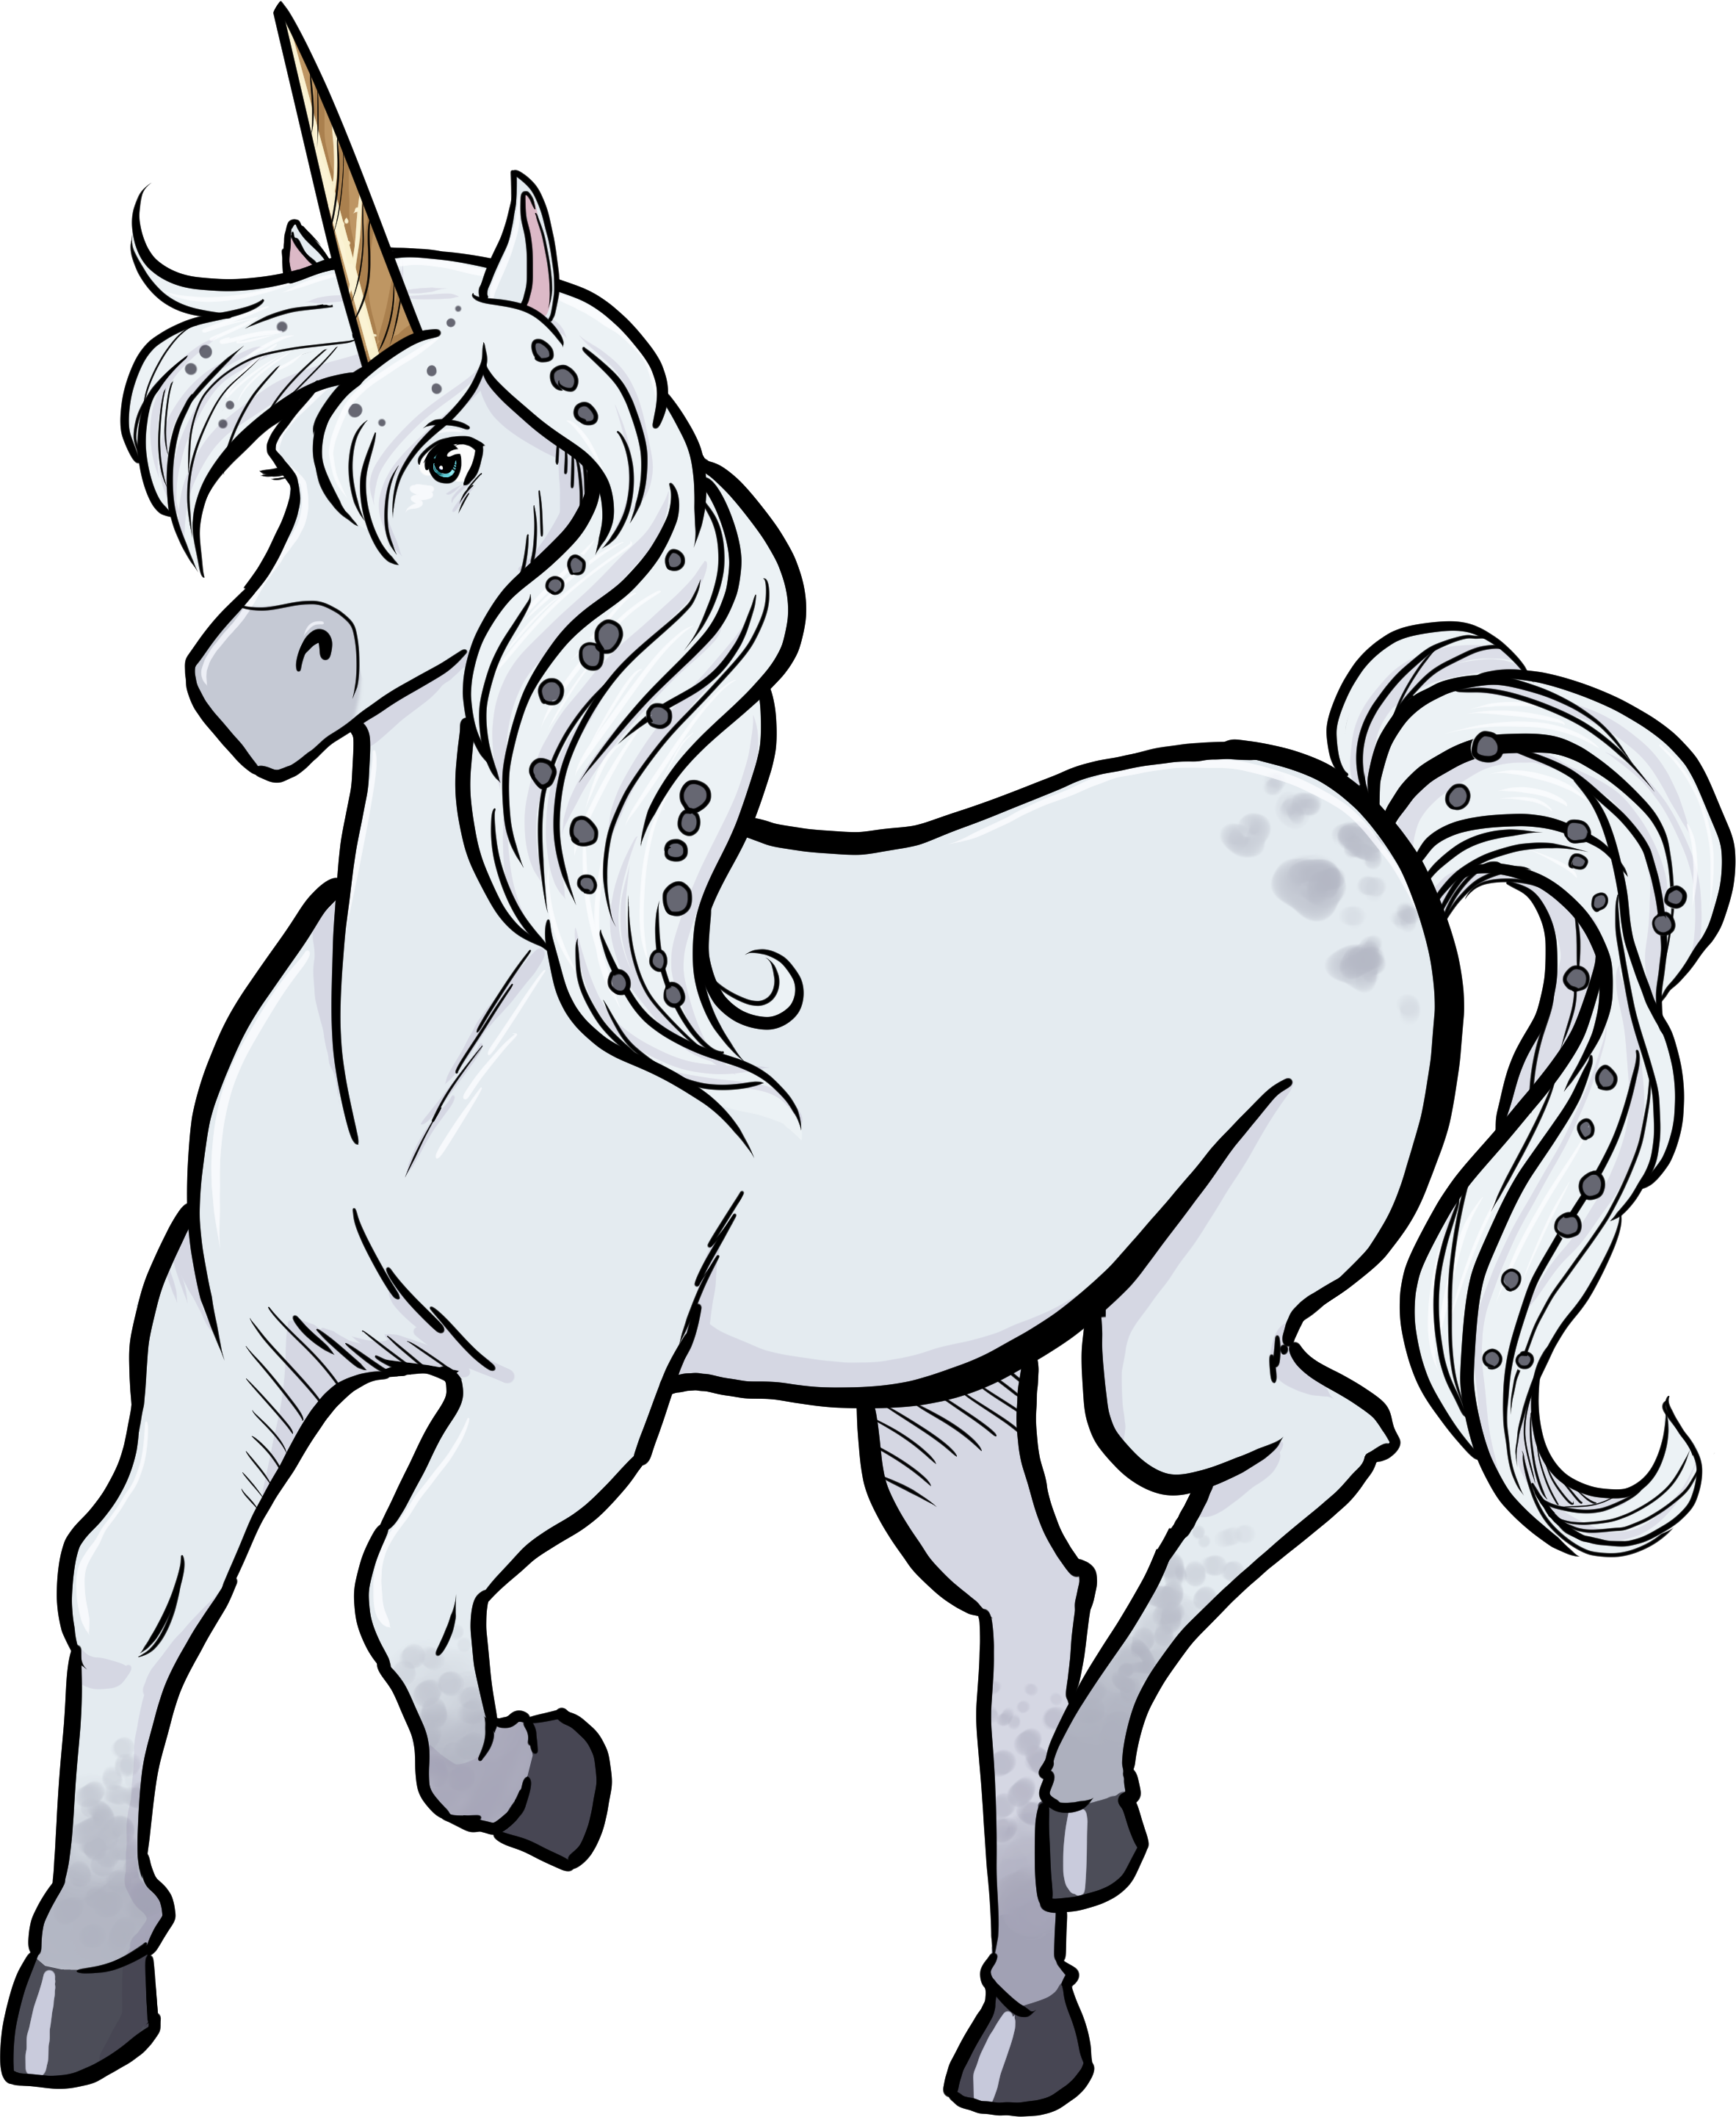
\includegraphics[width=\columnwidth]{Monsters/Unicorn}

\textbf{Teleport:} A unicorn can teleport up to 360 feet (with a rider) once per day.

\subsection{Vampire}\index[monsters]{Vampire}
\statblock{\textbf{Size:} Medium

\textbf{Type:} Undead

\textbf{Habitat:} Any (Rare)

\textbf{Wandering Group:} 1d4 (Nil)

\textbf{Lair Group:} 1d6 (F)

\textbf{Move:} 40 ft., 60 ft. (Fly)

\textbf{Armor Class:} 2

\textbf{Hit Dice:} 8** (36 HP)

\textbf{Attacks:} Touch (1d10)

\textbf{Special:} Charm Person, Create Spawn, 

Energy Drain (Human Form), 

Immunity (Mind Effects, Normal Weapons, Poison), 

Regeneration (3), Shapechange, Summon Animals, 

Vulnerability to Stakes, Vulnerability to Sunlight, 

Vulnerability to Water, Wards

\textbf{Save:} F8

\textbf{Alignment:} Chaotic

\textbf{Intelligence:} 10

\textbf{Morale:} 11

\textbf{XP Value:} 1,750}

\parbox{\columnwidth}{
	\begin{wrapfigure}{r}{0.5\columnwidth}
	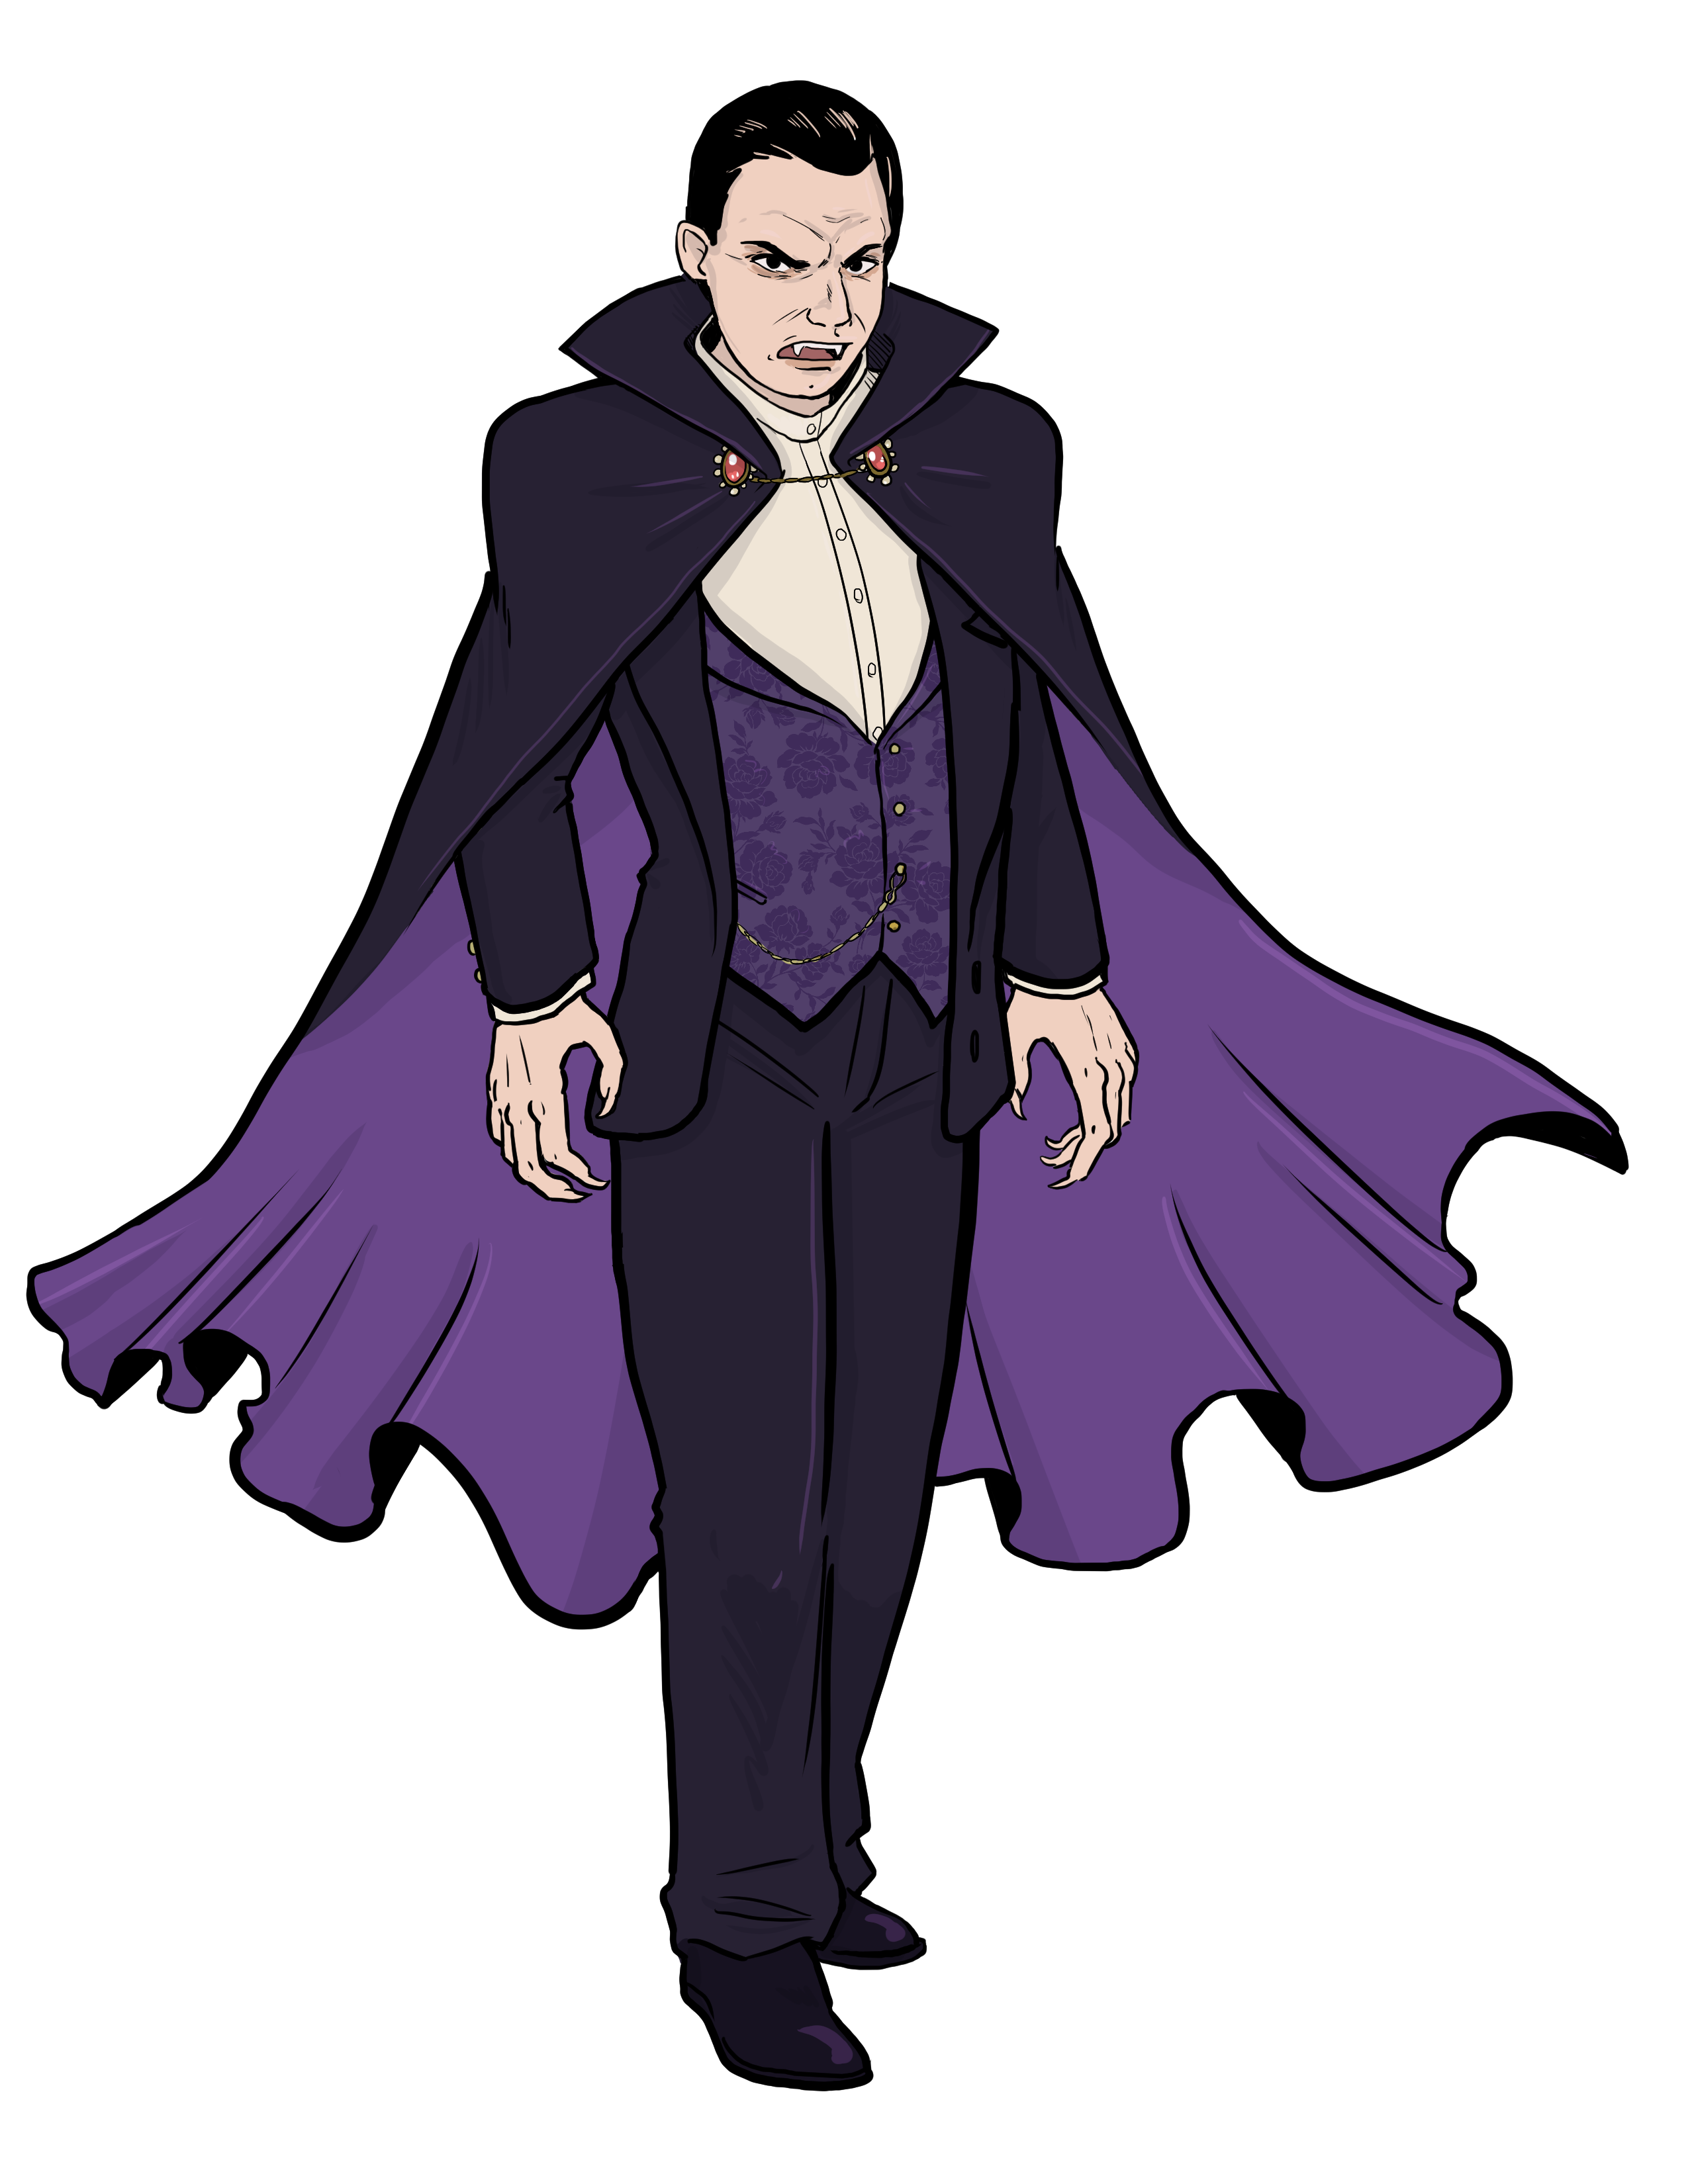
\includegraphics[width=\columnwidth]{Monsters/Vampire}
\end{wrapfigure}

Vampires are undead creatures that drink the blood of the living. Of all the undead, they are the ones that are most likely to be able to pass for living creatures, since other than their fangs they do not look different from when they were alive.

Vampires need to drink the blood of the living, and usually do so to charmed victims. The amount of blood actually drunk is not enough to cause harm to the victim, and the act of drinking does not break the charm.

Vampires must sleep in their coffins during the day, taking 2d6 damage (that can’t be regenerated) each time they miss a day. 
}

\textbf{Charm Person:} A vampire can cast a Charm Person spell at will, with a -2 penalty on the saving throw.

\textbf{Create Spawn:} Any human or demi-human killed by a vampire will rise in three days time as a vampire themselves, unless they have a Dispel Evil cast on them or they are raised.

\textbf{Energy Drain:} In human form, a vampire can touch to inflict 1d10 points of damage and a double strength \iref[sec:Energy Drain]{Energy Drain}, causing the target to lose two levels. This touch attack is optional, and the vampire does not have to use it (if pretending to still be alive, for example).

\textbf{Regeneration:} Vampires regenerate 3 hit points per round until slain. If a vampire is reduced to 0 hit points, it can no longer regenerate and must change to smoke form and return to its coffin where it will revert to human form and be unconscious for a full day.

\textbf{Shapechange:} A vampire may take the form of a dire wolf, giant bat, or cloud of smoke.

When in the form of a dire wolf or giant bat, the vampire’s movement, attacks and damage are the same as that of the animal.

In gaseous form, the vampire cannot attack but can fly and is immune to all weapons.

\textbf{Summon Animals:} A vampire may summon animals to its aid, but the animals will only respond if within 300 feet of the vampire. The animals can be either rats, bats or wolves. Giant or dire versions of the above will also answer the summons.

\textbf{Vulnerability to Stakes:} A vampire can be killed by driving a stake through its heart (not possible in combat, but possible when the vampire is sleeping or unconscious in its coffin).

\textbf{Vulnerability to Sunlight:} A vampire that is exposed to direct sunlight must make a saving throw vs. death ray each round or turn to ash.

\textbf{Vulnerability to Water:} A vampire can be killed by immersing it in running water for 10 minutes. They cannot cross running water except in their coffins or over a bridge.

\textbf{Wards:} Vampires cannot approach within 10 feet of a strongly presented holy symbol, even from a non-cleric; although they can attack from a different angle. They are repulsed by the smell of garlic, and must make a saving throw vs. poison to come within 10 feet of it.

\subsubsection{Spellcasting}
Vampires can be shamans (to \nth{9} level) or sorcerers (to \nth{9} level).



\subsection{Weasel, Giant}\index[monsters]{Giant Weasel}
\statblock{\textbf{Size:} Large

\textbf{Type:} Animal

\textbf{Habitat:} Underground, Woods (Common)

\textbf{Wandering Group:}  1d4 (Nil)

\textbf{Lair Group:} 1d6 (V)

\textbf{Move:} 50 ft.

\textbf{Armor Class:} 7

\textbf{Hit Dice:} 4+4 (34 HP)

\textbf{Attacks:} Bite (2d4)

\textbf{Special:} Drain Blood, Infravision, Scent

\textbf{Save:} F3

\textbf{Alignment:} None

\textbf{Intelligence:} 2

\textbf{Morale:} 8

\textbf{XP Value:} 125}

Giant weasels are long mammals covered with richly colored fur of brown, gold, or white.

\textbf{Drain Blood:} If a giant weasel’s bite succeeds, it will hold on to that victim and begin to drain their blood. The victim suffers 2d4 points of damage for every round their blood is being drained. The giant weasel will continue to drain the victim's blood until either the giant weasel or the victim is dies.

\textbf{Scent:} Giant weasels are able to pinpoint creatures and items within 30 feet by getting a sniff of their smell. Winds, weather conditions, and multiple strong odors may negate this ability.

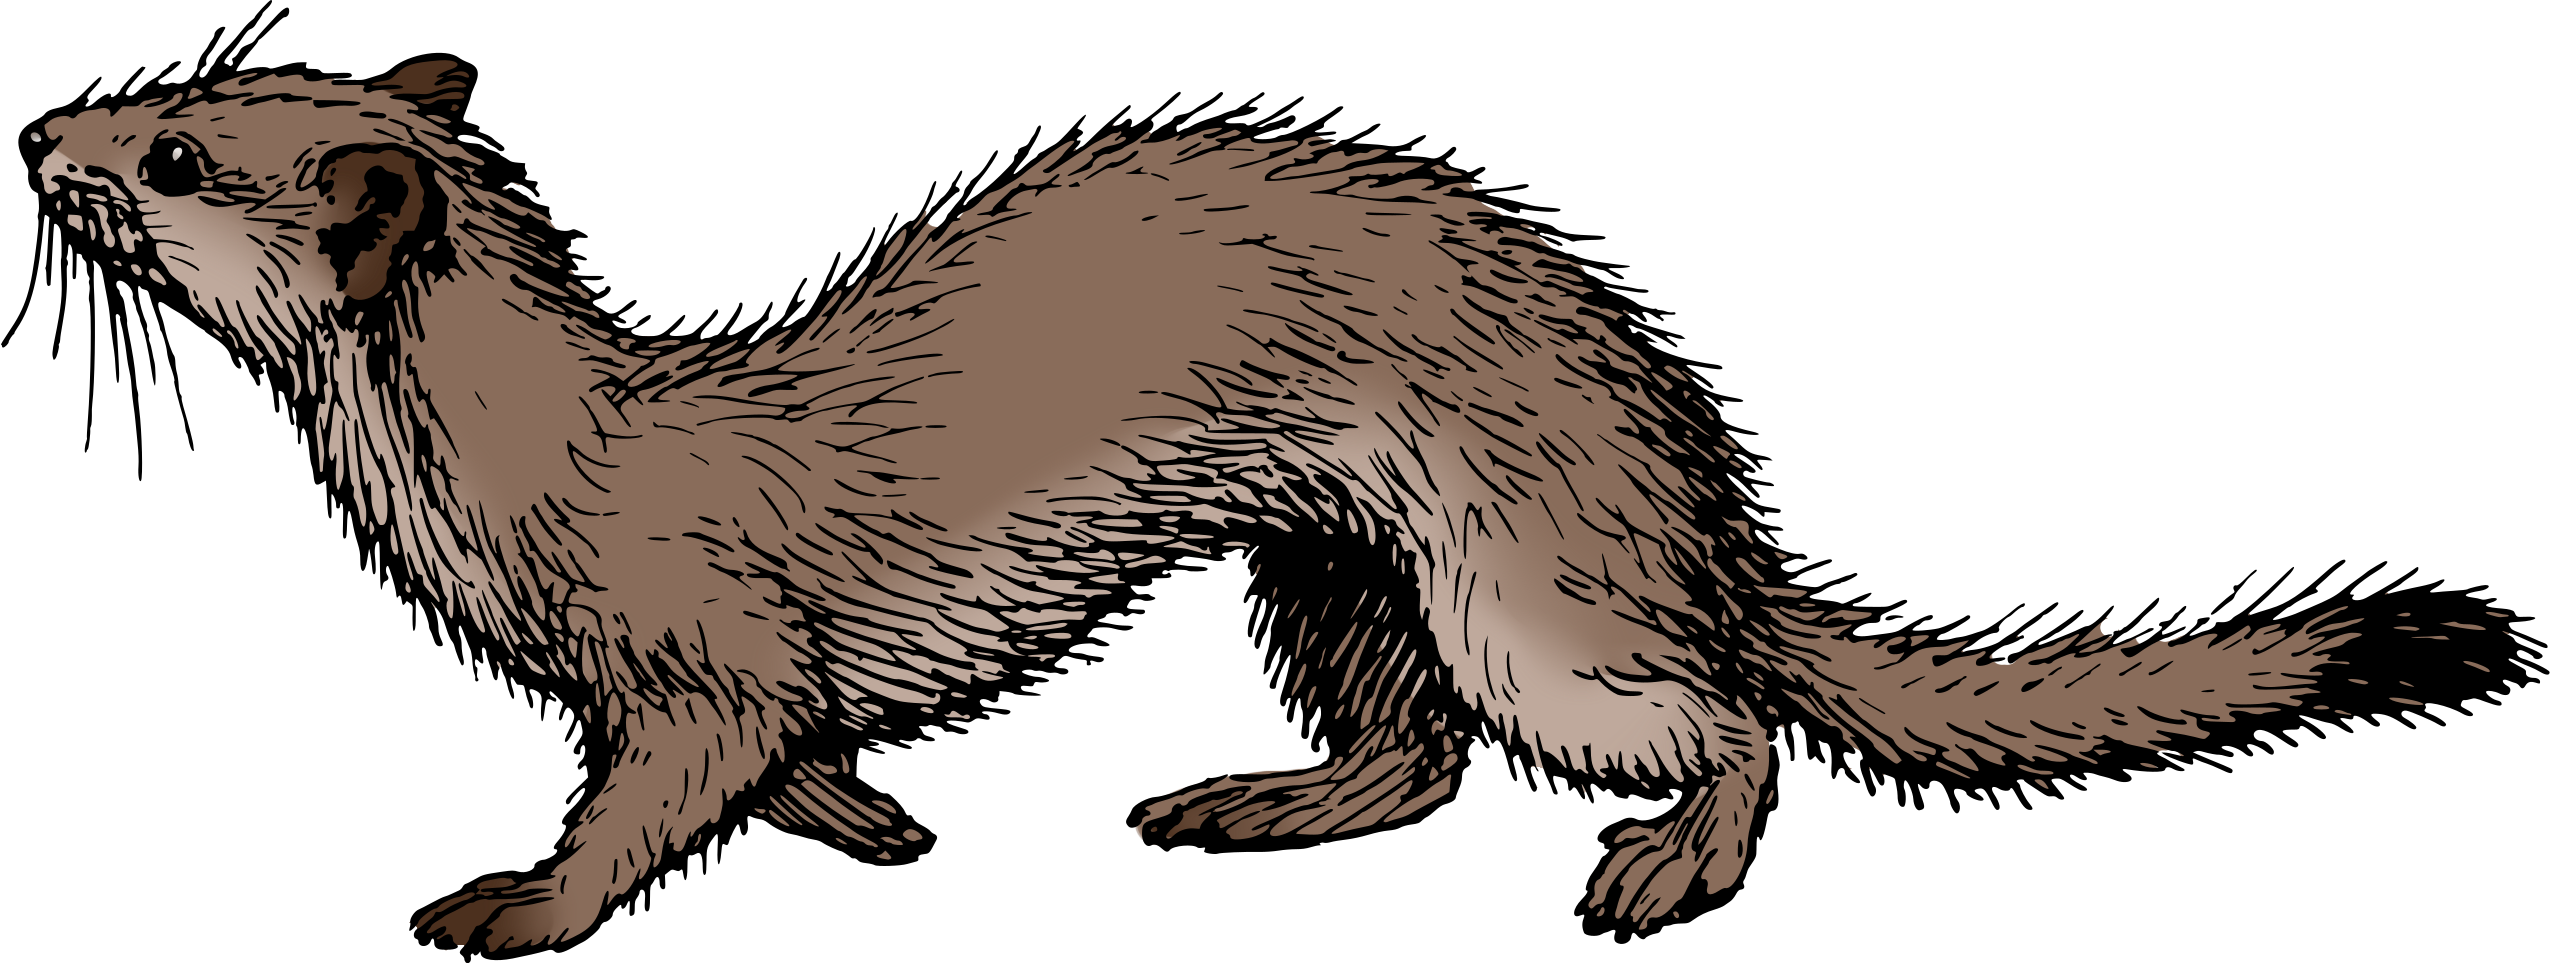
\includegraphics[width=\columnwidth]{Monsters/Animals/Weasel}

\subsection{Whale, Killer}\index[monsters]{Killer Whale}
\statblock{\textbf{Size:} Large

\textbf{Type:} Animal

\textbf{Habitat:} Ocean (Common)

\textbf{Wandering Group:} 1d6 (Nil)

\textbf{Lair Group:} 0 (Nil)

\textbf{Move:} 80 ft.

\textbf{Armor Class:} 6

\textbf{Hit Dice:} 6 (27 HP)

\textbf{Attacks:} Bite (2d10)

\textbf{Special:} Swallow Whole

\textbf{Save:} F3

\textbf{Alignment:} None

\textbf{Intelligence:} 4

\textbf{Morale:} 10

\textbf{XP Value:} 275}

Killer whales are seagoing mammals that are shaped like fish and have distinctive black and white markings.

They are very intelligent hunters, and will often co-operate with other sea creatures such as merfolk.

\textbf{Swallow Whole:} If a killer whale bites an opponent of \iref[class:Halfling]{Halfling} size or smaller with a natural roll of 20, the opponent is swallowed. Swallowed creatures take 1d6 damage per round and may drown (see \fullref{sec:Environmental Damage}).


\includegraphics[width=\columnwidth]{Monsters/Animals/Whale, Killer}

\subsection{Wight}\index[monsters]{Wight}
\statblock{\textbf{Size:} Medium

\textbf{Type:} Undead

\textbf{Habitat:} Barren Land, Underground (Common)

\textbf{Wandering Group:} 1d6 (Nil)

\textbf{Lair Group:} 1d8 (B)

\textbf{Move:} 30 ft.

\textbf{Armor Class:} 5

\textbf{Hit Dice:} 3* (14 HP)

\textbf{Attacks:} Touch (Special)

\textbf{Special:} Energy Drain, Immunity 

(Mind Effects, Non-Silver Normal Weapons, Poison)

\textbf{Save:} F3

\textbf{Alignment:} None

\textbf{Intelligence:} 5

\textbf{Morale:} 12

\textbf{XP Value:} 50}

Wights are undead that look much like they did in life, but shriveled and with hollow eyes.

Wights have little memory of their life, but may recognize a friend or family member and temporarily refrain from attacking them as they are confused by their memories.

\textbf{Energy Drain:} The touch of a wight does an \iref[sec:Energy Drain]{Energy Drain} to the victim, draining a single level. Any humanoid killed by a wight in this manner will become a wight themselves in 1d4 days unless a Dispel Evil is cast on them or they are raised.

\subsection{Wolf}\index[monsters]{Wolf}
\statblock{\textbf{Size:} Medium

\textbf{Type:} Animal

\textbf{Habitat:} Woods (Common)

\textbf{Wandering Group:} 2d6 (Nil)

\textbf{Lair Group:} 3d6 (Nil)

\textbf{Move:} 60 ft.

\textbf{Armor Class:} 7

\textbf{Hit Dice:} 2+2 (11 HP)

\textbf{Attacks:} Bite (1d6)

\textbf{Special:} None

\textbf{Save:} F1

\textbf{Alignment:} None

\textbf{Intelligence:} 2

\textbf{Morale:} 8

\textbf{XP Value:} 25}

Wolves are wild cousins of dogs. They are intelligent carnivores and hunt using pack tactics.

Although not domesticated like dogs, wolves are sometimes reared by humanoid races as guard or hunting animals.

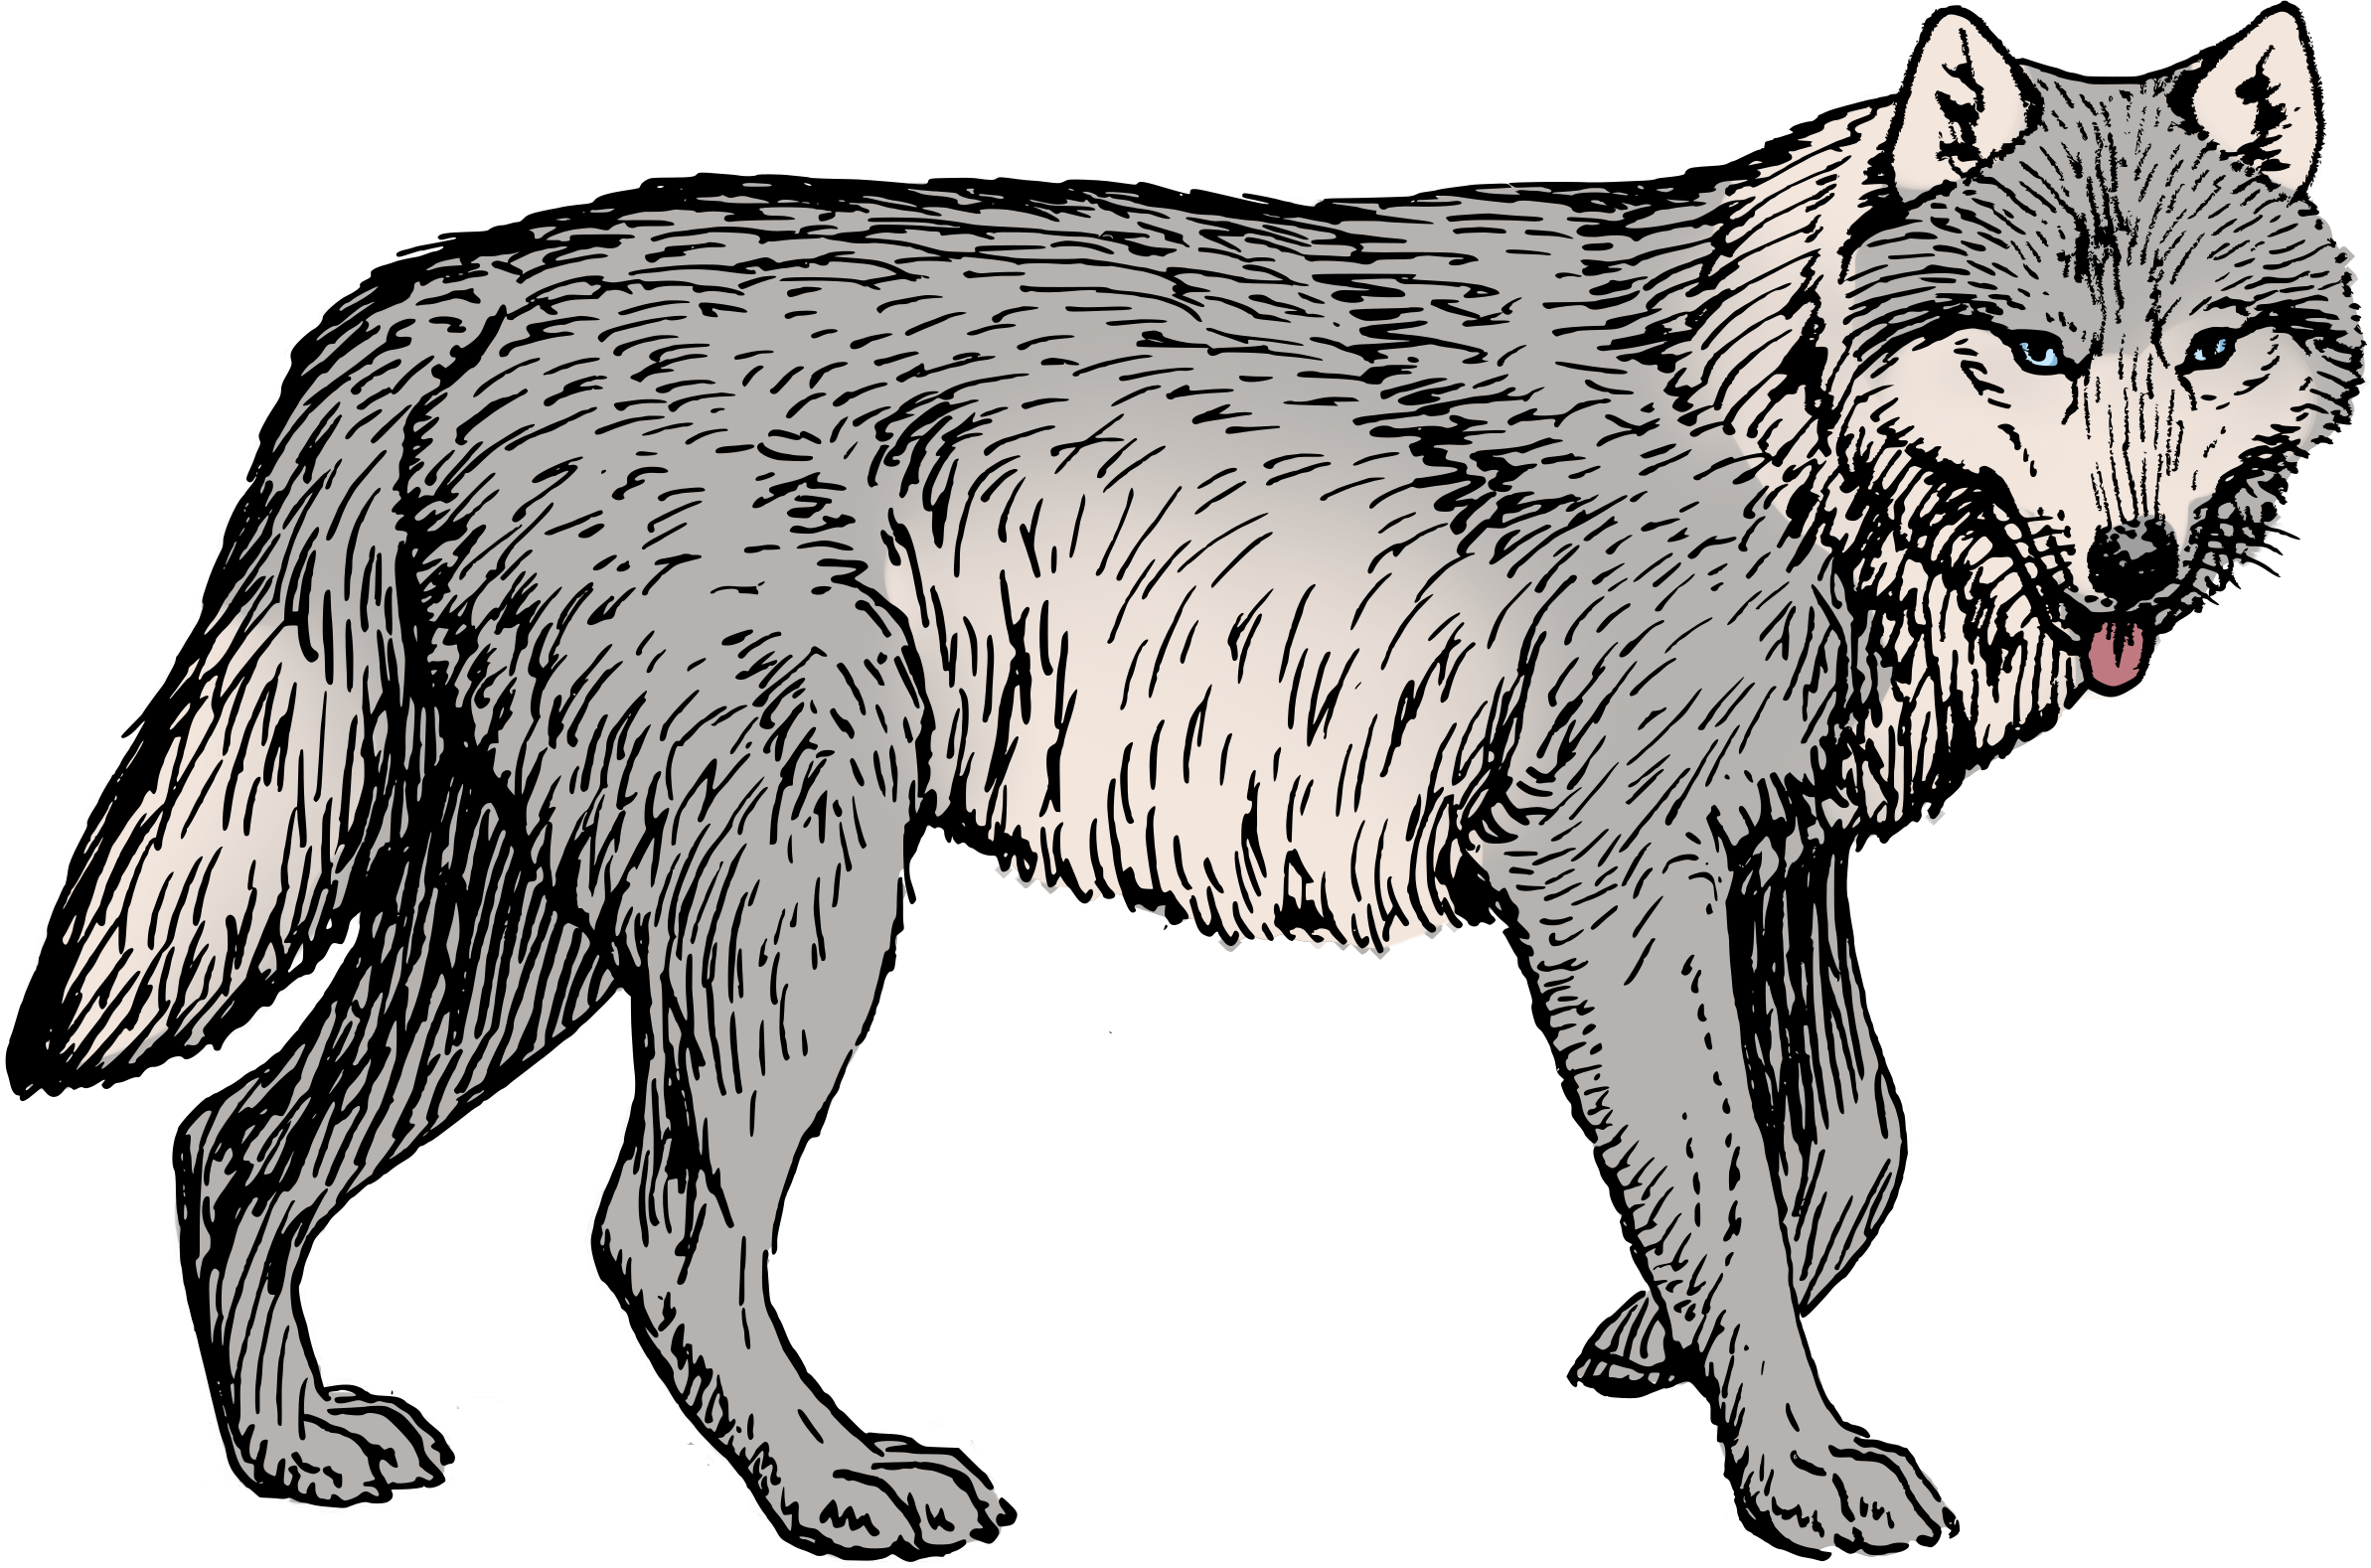
\includegraphics[width=\columnwidth]{Monsters/Animals/Wolf}

\subsection{Wolf, Dire}\index[monsters]{Dire Wolf}\label{monster:Dire Wolf}
\statblock{\textbf{Size:} Large

\textbf{Type:} Animal

\textbf{Habitat:} Woods (Rare)

\textbf{Wandering Group:} 1d4 (Nil)

\textbf{Lair Group:} 2d4 (Nil)

\textbf{Move:} 50 ft.

\textbf{Armor Class:} 6

\textbf{Hit Dice:} 4+1 (19 HP)

\textbf{Attacks:} Bite (2d4)

\textbf{Special:} None

\textbf{Save:} F2

\textbf{Alignment:} None

\textbf{Intelligence:} 4

\textbf{Morale:} 8

\textbf{XP Value:} 125}

Dire wolves are larger and more intelligent cousins of normal wolves.

Dire wolves hunt in packs like their smaller cousins.

Dire wolves are sometimes used by goblins as mounts.

\subsection{Worm, Cthonic}\index[monsters]{Cthonic Worm}
\statblock{\textbf{Size:} Large

\textbf{Type:} Monster

\textbf{Habitat:} Underground (Common)

\textbf{Wandering Group:} 1 (Nil)

\textbf{Lair Group:} 1d4 (B)

\textbf{Move:} 40 ft.

\textbf{Armor Class:} 7

\textbf{Hit Dice:} 3+1* (15 HP)

\textbf{Attacks:} 8x Tentacle (Special) or Bite (1 point)

\textbf{Special:} Paralyzing Touch

\textbf{Save:} F2

\textbf{Alignment:} None

\textbf{Intelligence:} 0

\textbf{Morale:} 9

\textbf{XP Value:} 75}

A cthonic worm is a hideous creature that looks like a cross between a worm and a squid. Its worm-like body is thick at the front and tapers off towards the rear. The front of the creature has no visible sensory organs, only a beak-like mouth surrounded by a ring of 5-foot-long slime-covered tentacles.

Despite the lack of visible sensory organs, Cthonic worms do have eyes under their skin and use normal vision to detect their prey.

Cthonic worms will eat anything organic, and will normally attack victims with their tentacles attempting to paralyze them with their poisonous slime.

The beak of a cthonic worm is weak, and will not be used for attack except in emergencies (for example in self-defense against creatures immune to paralysis) or to eat paralyzed victims.

A cthonic worm will not try to eat paralyzed victims while there are still mobile ones actively fighting it.

\textbf{Paralyzing Touch:} Anyone hit by cthonic worm's tentacle must make a saving throw vs. paralyzation or be paralyzed for 2d5x10 minutes.

\subsection{Worm, Purple}\index[monsters]{Purple Worm}
\statblock{\textbf{Size:} Large

\textbf{Type:} Monster

\textbf{Habitat:} Swamp, Underground, Woods (Very Rare)

\textbf{Wandering Group:} 1d2 (Nil)

\textbf{Lair Group:} 1d4 (D)

\textbf{Move:} 20 ft.

\textbf{Armor Class:} 6

\textbf{Hit Dice:} 15* (68 HP)

\textbf{Attacks:} Bite (2d8) \& Sting (1d8)

\textbf{Special:} Poison, Swallow Whole

\textbf{Save:} F8

\textbf{Alignment:} None

\textbf{Intelligence:} 0

\textbf{Morale:} 10

\textbf{XP Value:} 2,700}

A purple worm is a slimy worm-like creature. Purple worms tunnel through the earth, and rise to the surface to feed.

\textbf{Poison:} Anyone stung by a purple worm must make a saving throw vs. poison or die; although if the purple worm is encountered underground it is likely that it can not use its stinger in combat as it will not have room to maneuver.

\textbf{Swallow Whole:} If a purple worm bites an opponent of human-sized or smaller, and its to-hit roll is at least 4 more than it needs to be to hit, or is a natural 20, then it will swallow the victim whole. Swallowed creatures take 3d6 damage per round until the purple worm is killed.

\subsection{Wraith}\index[monsters]{Wraith}
\statblock{\textbf{Size:} Medium

\textbf{Type:} Undead

\textbf{Habitat:} Barren Land, Underground (Rare)

\textbf{Wandering Group:} 1d4 (Nil)

\textbf{Lair Group:} 1d6 (E)

\textbf{Move:} 40 ft., 80 ft. (Fly)

\textbf{Armor Class:} 3

\textbf{Hit Dice:} 4** (18 HP)

\textbf{Attacks:} Claw (1d6)

\textbf{Special:} Create Spawn, Energy Drain, Immunity 

(Mind Effects, Non-Silver Normal Weapons, Poison)

\textbf{Save:} F4

\textbf{Alignment:} Chaotic

\textbf{Intelligence:} 7

\textbf{Morale:} 11

\textbf{XP Value:} 175}

Wraiths are incorporeal undead, appearing as semi-transparent hooded figures with no visible faces or legs, but with skeletal hands emerging from their robes.

\textbf{Create Spawn:} Anyone killed by a wraith will rise as a wraith themselves the following night unless a Dispel Evil or Raise Dead spell is cast on them.

\textbf{Energy Drain:} Anyone clawed by a wraith is subject to an \iref[sec:Energy Drain]{Energy Drain} that drains them of one level of experience.

\subsection{Wyvern}\index[monsters]{Wyvern}
\monsterimage{Monsters/Wyvern}{\statblock{\textbf{Size:} Large

\textbf{Type:} Dragon

\textbf{Habitat:} Mountains, Woods (Rare)

\textbf{Wandering Group:} 1d2 (Nil)

\textbf{Lair Group:} 1d6 (E)

\textbf{Move:} 30 ft., 80 ft. (Fly)

\textbf{Armor Class:} 3

\textbf{Hit Dice:} 7* (32 HP)

\textbf{Attacks:} Bite (2d8) \& Sting (1d6)

\textbf{Special:} Poison

\textbf{Save:} F4

\textbf{Alignment:} None

\textbf{Intelligence:} 3

\textbf{Morale:} 9

\textbf{XP Value:} 850}}

Wyverns are winged reptilian creatures with two legs and a long neck and tail. They vaguely resemble dragons, and may be mistaken for them when flying at a distance, but the two are not related.

Wyverns are carnivorous, and in combat they use both their bite and the stinger on their tail, which is flexible enough to reach around in front of them.

\textbf{Poison:} Anyone stung by a wyvern must make a saving throw vs. poison or die.

\subsection{Yellow Mold}\index[monsters]{Yellow Mold}
\statblock{\textbf{Size:} Large

\textbf{Type:} Plant

\textbf{Habitat:} Underground (Common)

\textbf{Wandering Group:} 0 (Nil)

\textbf{Lair Group:} 1d4 (Nil)

\textbf{Move:} -

\textbf{Armor Class:} Special

\textbf{Hit Dice:} 2* (9 HP)

\textbf{Attacks:} None

\textbf{Special:} Spore Cloud

\textbf{Save:} F2

\textbf{Alignment:} None

\textbf{Intelligence:} 0

\textbf{Morale:} 12

\textbf{XP Value:} 25}

Yellow mold is a fungus that grows virulently in damp underground environments. Each “monster” represents a 10-by-10-foot area of mold, and more than one may be found next to each other.

Yellow mold looks like a bright yellow slimy fibrous growth, with many small ball shaped fungal pods in it. These pods are reproductive organs and contain the spores that yellow mold uses to grow and colonize new areas.

Yellow mold can only be killed by burning it.

\textbf{Spore Cloud:} If anything touches a yellow mold (including flame) there is a 50\% chance that it will release a cloud of spores in a 10 by 10 by 10 foot area around itself. Any creature caught in the area will take 1d6 damage and must make a saving throw vs. death ray or choke to death in 6 rounds.

A Cure Disease spell will kill the spores in a person’s throat and lungs, stopping their choking, but will not kill a fully grown patch of mold.

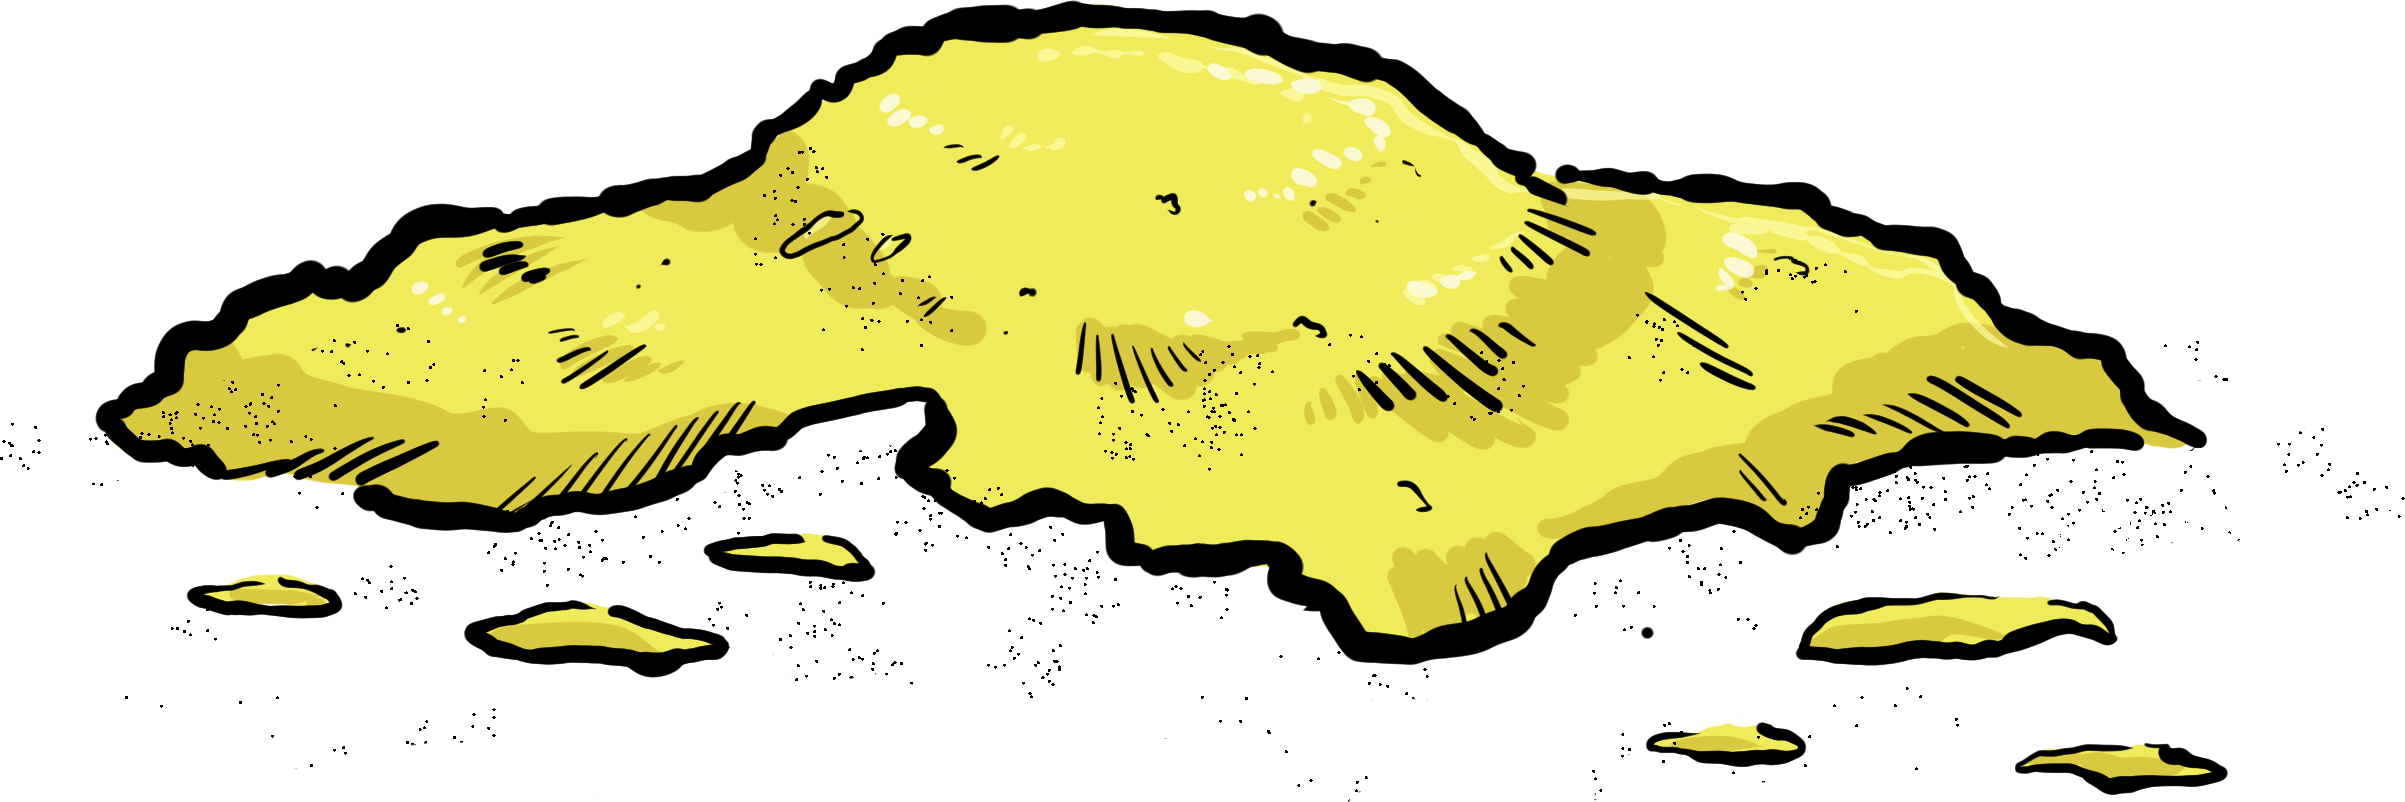
\includegraphics[width=\columnwidth]{Monsters/Yellow Mold}

\subsection{Zombie}\index[monsters]{Zombie}
\monsterimage{Monsters/Zombie}{
\statblock{\textbf{Size:} Medium

\textbf{Type:} Undead

\textbf{Habitat:} Underground (Common)

\textbf{Wandering Group:} 2d4 (Nil)

\textbf{Lair Group:} 4d6 (Nil)

\textbf{Move:} 30 ft.

\textbf{Armor Class:} 8

\textbf{Hit Dice:} 2 (9 HP)

\textbf{Attacks:} Claw (1d8) or 

Weapon (By weapon)

\textbf{Special:} Immunity 

(Mind Effects, Poison)

\textbf{Save:} F1

\textbf{Alignment:} None

\textbf{Intelligence:} 1

\textbf{Morale:} 12

\textbf{XP Value:} 20}}

Zombies are mindless undead created by an Animate Dead spell.

Although tougher than skeletons, zombies are slower and more mindless, following orders literally with absolutely no sense of self-preservation.

Zombies are slow fighters, and always lose initiative.

\end{multicols*}

